\documentclass[a4paper, 12pt]{scrreprt}
\usepackage[utf8]{inputenc}
\usepackage{graphicx} % Required for inserting images
\usepackage{minted}
\usepackage{csquotes}
\usepackage{amsmath}
\usepackage{geometry}
\usepackage[ngerman]{babel}
\usepackage{amssymb}
\usepackage{pdfpages}
\usepackage{array}
\usepackage{svg}
\usepackage{booktabs} 
\usepackage{comment}

\everymath{\displaystyle}

\DeclareMathOperator*{\argmax}{arg\,max}
\DeclareMathOperator*{\argmin}{arg\,min}

\setminted[python]{fontsize=\footnotesize}
\setmintedinline{fontsize=\currentfontsize}

\setcounter{secnumdepth}{4}

\usepackage[backend=biber,sorting=ynt]{biblatex}
\addbibresource{lib.bib}

\title{Bachelorthesis}
\author{Marlon Zarnke}
\date{August 2024}

\newcommand*{\field}[1]{\mathbb{#1}}%

\usepackage{listings}
\usepackage{xcolor}

\definecolor{codegreen}{rgb}{0,0.6,0}
\definecolor{codegray}{rgb}{0.5,0.5,0.5}
\definecolor{codepurple}{rgb}{0.58,0,0.82}
\definecolor{backcolour}{rgb}{0.95,0.95,0.92}
\lstdefinestyle{mystyle}{
    backgroundcolor=\color{backcolour},   
    commentstyle=\color{codegreen},
    keywordstyle=\color{magenta},
    numberstyle=\tiny\color{codegray},
    stringstyle=\color{codepurple},
    basicstyle=\ttfamily\footnotesize,
    breakatwhitespace=false,         
    breaklines=true,                 
    captionpos=b,                    
    keepspaces=true,                 
    numbers=left,                    
    numbersep=5pt,                  
    showspaces=false,                
    showstringspaces=false,
    showtabs=false,                  
    tabsize=2
}

\lstset{style=mystyle}

\begin{document}
\newpage
\thispagestyle{empty}

\includepdf[pages=1]{pdf/Thesis_Bachelor-WS 2024-Marlon Zarnke.pdf}

\newpage

\pagenumbering{roman}
\setcounter{page}{1}

\begin{center}
\textbf{Eidesstattliche Erklärung}\\
Ich erkläre, dass ich die Arbeit selbstständig angefertigt und nur die angegebenen
Hilfsmittel benutzt habe. Alle Stellen, die dem Wortlaut oder dem Sinn nach anderen
Werken, gegebenenfalls auch elektronischen Medien, entnommen sind, sind von mir
durch Angabe der Quelle als Entlehnung kenntlich gemacht. Dies gilt auch für
Zeichnungen, Skizzen, Bilder und andere visuelle Darstellungen.\\
Karlsruhe, 23.01.2025, Marlon Zarnke
\end{center}



\newpage
\begin{center}
\underline{\textbf{Danksagung}}\\
An dieser Stelle möchte ich mich bei all denjenigen bedanken, die mich während der Entstehung dieser Arbeit unterstützt haben. Mein besonderer Dank gilt meinem Betreuer, Philipp Reis, für seine Zeit, die kontinuierliche Betreuung sowie sein wertvolles Feedback und die Anregungen zur Durchführung dieser Arbeit. Diese haben mir sehr geholfen, die Arbeit in die richtige Richtung zu lenken. Ebenso danke ich ihm für die umfassende Unterstützung bei der Durchführung der Untersuchungen sowie für die Beantwortung und Klärung offener Fragen meinerseits.

Ein herzliches Dankeschön auch an meine Familie, deren Geduld\\
und Unterstützung mir in dieser herausfordernden Zeit sehr geholfen haben.

Ohne die Hilfe all dieser Menschen wäre diese Arbeit nicht in der vorliegenden Form möglich gewesen. Ich danke allen sehr für ihre Unterstützung.
\end{center}

\tableofcontents

\newpage
\pagenumbering{arabic}
\setcounter{page}{1}

\chapter{Einleitung}
    In der heutigen Zeit rückt das autonome Fahren immer mehr in den Vordergrund, was aus Nachrichten und veröffentlichten Berichten der Medien bekannt ist \cite{autonom}. Zwischen Theorie und Praxis existieren dennoch verschiedene Probleme, die eigenständige Lösungsansätze erfordern. 
    Ein Auto, das vollständig automatisiert fahren soll, muss sehr große Mengen an Daten aus der Umgebung erfassen. Dazu zählen Sensordaten über das Fahrzeug selbst, wie Geschwindigkeit, Reifendruck oder GPS-Daten und insbesondere große Mengen an Bilddaten. Bilddaten machen mit Abstand den größten Speicherbedarf aus (Reis, Philipp, 2024, Mitarbeiter am FZI) \cite{overload}.
    
    Häufig sollen diese Daten zur Weiterverarbeitung oder für analytische Zwecke in eine Cloud übertragen werden, da eine Verarbeitung vor Ort nicht effizient ist. Zudem ist es kostspielig, jedes Auto mit zusätzlicher Hardware auszustatten, um solche Datenmengen effizient zu verarbeiten. Ein weiterer Aspekt ist, dass die Daten ansonsten auf die einzelnen Autos verteilt wären. Es ist jedoch deutlich einfacher, die Daten in einem einzigen Rechenzentrum zu bündeln.
    Amazon Web Services oder Microsoft Azure bieten praktische Lösungen, um Daten sicher in einer gehosteten Cloud auszulagern. Die Automobilindustrie, welcher die Fahrzeuge gehören, kann natürlich auch firmeninterne Server verwenden, um die Daten dort zu sichern, auf einem zentralen Server. Aufgrund der großen Menge an Daten ist dies in der Praxis jedoch keine triviale Aufgabe.
    
    Am Forschungszentrum Informatik (FZI) gibt es praktische Versuche mit einem Audi, welcher bezeichnet wird als „CoCar NextGen“, das mit entsprechenden Kameras ausgestattet ist und während der Fahrt Bilddaten aufzeichnet.
    Diese werden von bis zu neun hochauflösenden HD-Kameras, die am Auto installiert sind, aufgezeichnet, um die Umgebung möglichst präzise, $360^\circ$ um das Auto herum abzubilden, was zu großen Datenmengen führt \cite{fzi_car}. 
    
    Allein an Bilddaten entstehen bei neun HD-Kameras, welche mit $30$ FPS und einer Farbtiefe von $24$-Bit aufzeichnen würden $13,41$ GBit/s –\\ das sind etwa $1$ TB nach nur $10$ Minuten Fahrt. Diese Daten während der Fahrt in die Cloud hochzuladen, erfordert viel Bandbreite. Dafür ist die Upload-Geschwindigkeit oft zu gering, und der Speicher im Fahrzeug würde sich schnell füllen \cite{overload}.
    
\newpage 
    Die Reduktion und Rekonstruktion von Daten ist ein Lösungsansatz, um dieses Problem der Praxis des autonomen Fahrens zu beheben.
    Komprimierte Daten sind speichersparender und können anschließend in die Cloud hochgeladen werden, wo sie weiterverarbeitet werden.
    Dies kann durch herkömmliche Komprimierung, wie verlustbehaftete Bildformate, erfolgen oder mithilfe von KI-Modellen, die die Daten komprimieren, um sie in die Cloud hochzuladen. Anschließend können sie von einem spezialisierten Modell rekonstruiert werden, das für die Wiederherstellung der Bilder optimiert ist. Die rekonstruierten Bilder sollten dabei dem Original so genau wie möglich entsprechen.

    Diese Arbeit stellt sich die Frage, inwieweit sich verlustbehaftete sowie rekonstruierte Daten von den Originalen unterscheiden und ob auf Basis dieser immer noch gleiche Aussagen getroffen werden können.

    Die Struktur der Arbeit gliedert sich in ein Grundlagenverständnis und eine Übersicht der verwandten Arbeiten (Related Work) sowie einen Einblick in das Konzept, das umgesetzt wird. Für die Evaluation werden Bilder eines zur Domäne passenden Datensatzes, die unterschiedlichen Kompressionsstufen unterzogen wurden (sowohl traditionelle als auch KI-basierte Kompression), miteinander und untereinander verglichen. Dies erfolgt anhand verschiedener Metriken, um eine fundierte Auswertung zu ermöglichen. Zudem wird ein KI-Modell eingesetzt, um die Bilder auf Objektdetektion zu überprüfen. Aus den Ergebnissen werden Schlussfolgerungen gezogen, ob es Abhängigkeiten, Gemeinsamkeiten oder Kausalitäten gibt.
\chapter{Grundlagen}
    \section{Supervised Learning}
        \cite{supervised} Beim Supervised Learning gibt es sogenannte Features (Eingabedaten) \textbf{x}
        und Labels (Zielvariablen) \textbf{y}.
        Die Daten bestehen also aus Features und den dazugehörigen Labels.
        Ein Modell, welches diese Eingabedaten zum Trainieren erhält, versucht nun, einen Zusammenhang zwischen den Features und den Labels zu erkennen.
        Ein trainiertes Modell kann nun bei nicht gelabelten Eingabedaten das Label zu dem Datenpunkt, der dazugehört, vorhersagen.
        Supervised Learning zählt neben Unsupervised Learning und Reinforcement Learning zu einem der drei Teilaspekte, aus denen Machine Learning besteht.\\[2ex]
        Supervised Learning lässt sich unterteilen in zwei Arten:

        \begin{enumerate}
            \item Regression\\
                Zu einer Regression gehören alle Vorhersagen bei denen das Label kontinuierlich ist: $y \in \field{ R}$ \\
                Beispiele:
                \begin{itemize}
                    \item Vorhersage der Temperatur
                    \item Vorhersage des DAX
                    \item Vorhersage des Gewichts
                \end{itemize}
            \item Klassifizierung
                Vorhersagen bei denen das Label  Kategorisch ist, werden als Klassifizierung (Classification) bezeichnet.
                Es gibt zwei Arten von Klassifizierungen. Binäre Klassifizierung wenn es genau zwei Klassen gibt, sowie Mehrklassen-Klassifizierung.\\
                Beispiele:
                \begin{itemize}
                    \item 
                    \textbf{x}: Alle Pixel eines Bildes.\\
                    \textbf{y}: Welches Tier ist zu sehen? $y = 0$: "Katze", $y = 1$: "Hund", $y = 2$: "Maus" \\
                    $\rightarrow y \in \{0, 1, 2\}$
                    \item
                    \textbf{x}: Das Geschlecht einer Person \\
                    \textbf{y}: $y = 0$: Mann, $y = 1$: Frau \\
                    $\rightarrow y \in \{0, 1\}$
                \end{itemize}
        \end{enumerate}

\newpage
    \section{Unsupervised Learning} 
        \cite{unsupervised} Anders als beim Supervised Learning gibt es beim Unsupervised Learning keine Labels.
        Das Ziel besteht darin, innerhalb der Daten Strukturen und Muster zu erkennen.
        Es gibt verschiedene Arten des Unsupervised Learning.
        \begin{enumerate}
            \item Clustering
   
            Beim Clustering werden Datenpunkte in Gruppen unterteilt.
            Daten innerhalb einer Gruppe ähneln sich. Datenpunkte aus unterschiedlichen Gruppen weißen größere Unterschiede auf.
            \begin{figure}[!htb]
                \centering
                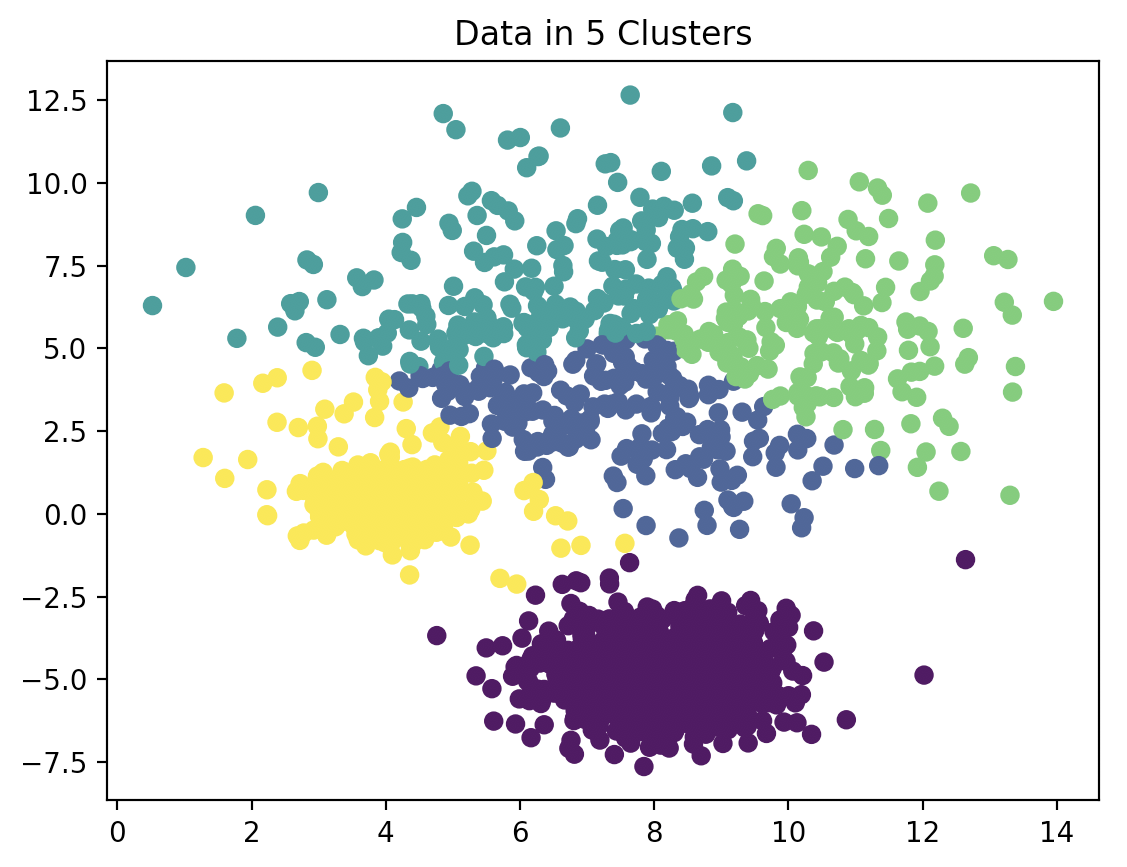
\includegraphics[scale=0.2]{pictures/k-means-clustering.png}
                \caption{Datenpunkte unterteilt in fünf Cluster \cite{k-means-clustering}.}
            \end{figure}
            \item Dimensionsreduktion

            Hierbei handelt es sich um Modelle, die Daten entgegennehmen und diese komprimieren.
            Dafür wird kein Label benötigt. Ein Beispiel ist ein Autoencoder, da dieser Daten komprimiert und anschließend wieder rekonstruiert. Hierfür werden lediglich die Features benötigt, jedoch keine Labels.
            Diese Art der Dimensionsreduktion wird im weiteren Verlauf dieses Kapitels genauer betrachtet.  
        \end{enumerate}

\newpage
    \section{Neural Networks}
        Ein neuronales Netz (Neural Network) ist eine Modellarchitektur,
        die aus sogenannten Neuronen und Schichten besteht.\\
        Es wird als „neuronales Netz“ bezeichnet, da es von den Gehirnen lebender Organismen inspiriert wurde.
        Gehirne besitzen ebenfalls Neuronen, die miteinander verbunden sind.
        Durch diese Verbindungen werden elektrische Signale geleitet, die das Denken ermöglichen.
        Ein neuronales Netz im Bereich der Informatik wird auch als künstliches neuronales Netz (KNN), englisch Artificial Neural Network (ANN), bezeichnet. Meist wird jedoch einfach die Abkürzung NN verwendet \cite{wikipedia_nn}.

        \subsection{Single-Layer Perceptrons}
            Die einfachste Form eines neuronalen Netzes ist ein einfaches Perzeptron (Single-Layer Perceptron). Es besteht aus zwei Schichten: der Eingabeschicht (Inputlayer), die für jeden Eingabepunkt ein Neuron enthält, und der Ausgabeschicht (Outputlayer), die aus einem Neuron für jede Ausgabe-Klasse besteht.
            Diese Art von Modellarchitektur gehört zum Supervised Learning.
            
            Single-Layer Perceptrons sind jedoch nur für sehr einfache Aufgaben geeignet,
            beispielsweise das Lernen einer logischen ODER- oder UND-Funktion.
            Single-Layer Perceptrons implementieren eine Binärklassifizierung, da es nur zwei Output-Neuronen gibt, 
            wie in Abbildung 1 zu sehen ist \cite{perceptrons}.
        
            \begin{figure}[!htb]
                \centering
                \includegraphics[width=11cm]{pictures/NN.pdf}
                \caption{Hier ist ein Single-Layer Perceptron zu sehen.}
            \end{figure}
        

\newpage
        \subsection{Deep Neural Networks}
            Tiefe neuronale Netze, im Englischen Deep Neural Networks (DNN), unterscheiden sich von Single-Layer Perceptrons darin, dass sie nicht nur eine Eingabeschicht und eine Ausgabeschicht besitzen, sondern auch versteckte Schichten (Hidden Layers) enthalten.
            Alle versteckten Schichten befinden sich zwischen der Eingabe- und der Ausgabeschicht.
            Ein DNN kann beliebig viele versteckte Schichten haben. Die Anzahl ist frei wählbar, es muss jedoch mindestens eine versteckte Schicht vorhanden sein, damit es als DNN gezählt wird.
            Die Anzahl der Neuronen in solchen versteckten Schichten kann ebenfalls beliebig variieren und ist somit ebenfalls frei wählbar.
            Je nach Design gibt es DNNs in den verschiedensten Größen und Komplexitätsstufen.
            Da die meisten neuronalen Netze versteckte Schichten besitzen, handelt es sich fast immer um DNN. Deshalb wird in der Regel einfach von neuronalen Netzen gesprochen, auch wenn DNNs gemeint sind. \newline
            \begin{figure}[!htb]
                \centering
                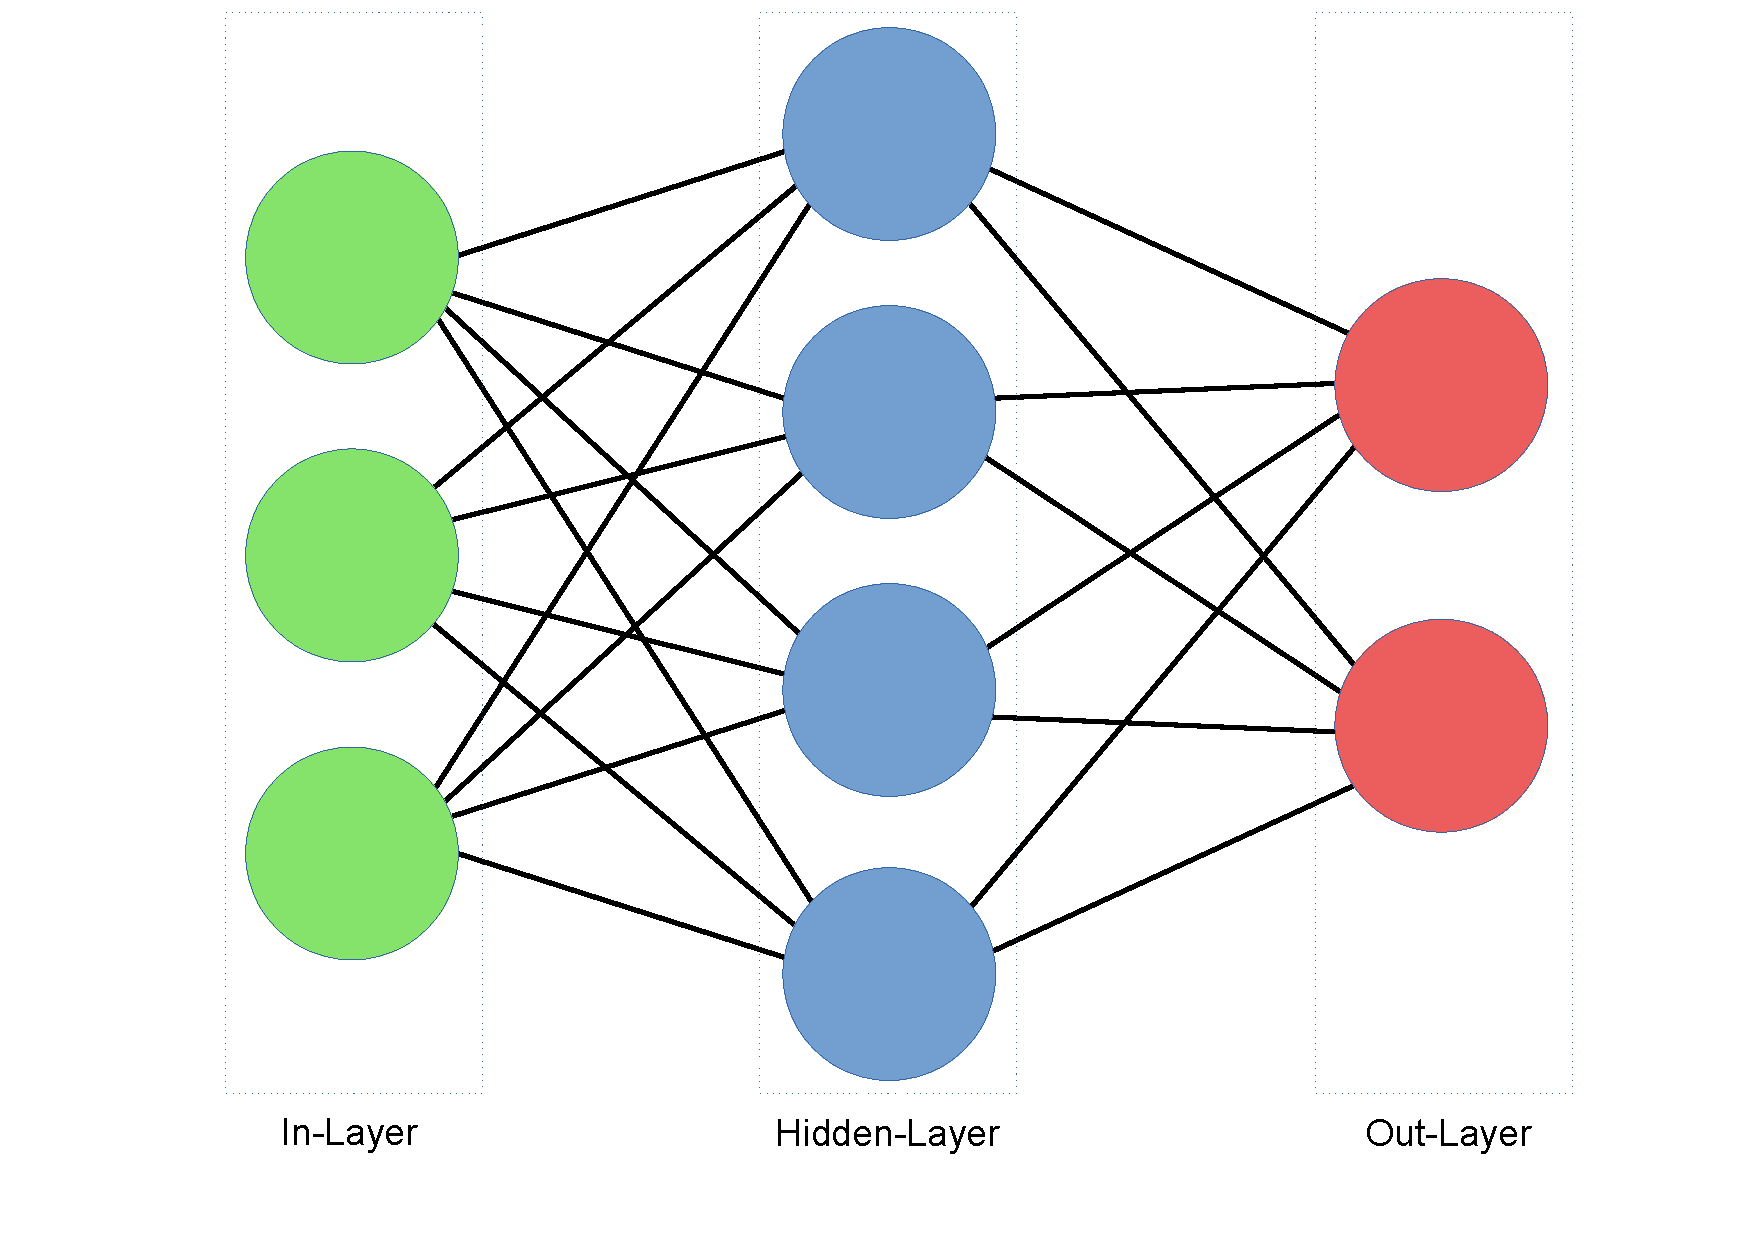
\includegraphics[width=11cm]{pictures/DNN.pdf}
                \caption{Hier ist ein Deep Neural Network mit einer versteckten Schicht zu sehen.}
            \end{figure}

\newpage
        \subsection{Convolutuional Neural Networks}
            \cite{convolutional} Convolutional Neural Networks (CNN) sind eine spezielle Architektur von
            künstlichen neuronalen Netzen, die besonders für die Verarbeitung von Daten mit räumlicher Struktur, wie z.B. Bildern, geeignet sind. Sie zeichnen sich durch den Einsatz von Faltungsschichten (Convolutional Layers) aus, die lokale Merkmale in den Eingabedaten extrahieren.
            Eine typische CNN-Architektur besteht aus drei Hauptkomponenten:

            \begin{enumerate}
                \item Convolutional Layers:\\
                    Diese Schichten führen die Faltung durch und erzeugen Feature Maps, die charakteristische Muster wie Kanten, Texturen oder Formen erkennen.
                \item Pooling Layers:\\
                    Diese Schichten reduzieren die räumliche Größe der Feature Maps und verringern so die Anzahl der Parameter, was die Berechnung effizienter macht und die Generalisierungsfähigkeit erhöht.
                \item Fully Connected Layers:\\
                    In diesen Schichten werden die extrahierten Merkmale für die Klassifikation oder andere Aufgaben genutzt.
            \end{enumerate} 
            
            CNNs sind bekannt für ihre Effektivität bei Aufgaben wie Bildklassifikation, Objekterkennung und Bildsegmentierung. Zu den erfolgreichsten Architekturen zählen Modelle wie AlexNet, VGG und ResNet, die sich durch fortschrittliche Designprinzipien und leistungsstarke Ergebnisse auszeichnen.

            Dank ihrer Fähigkeit, automatisch relevante Merkmale aus Rohdaten zu extrahieren, haben CNNs die Entwicklung in Bereichen wie Computer Vision, autonomes Fahren und medizinische Bildverarbeitung revolutioniert.

            \begin{figure}[!htb]
                \centering
                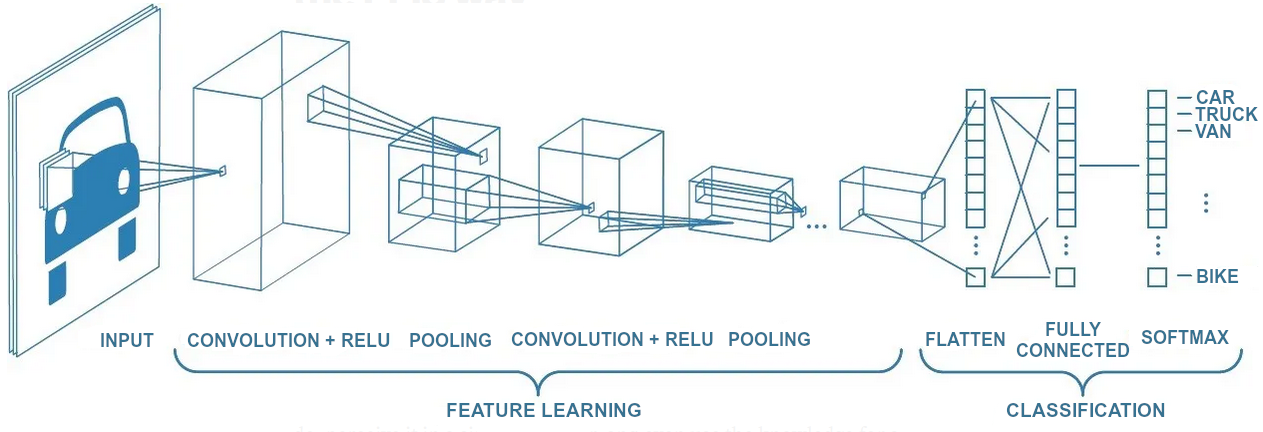
\includegraphics[scale=0.42]{pictures/cnn_auto.png}
                \caption{Visualisierung eines CNN \cite{cnn_auto}.}
            \end{figure}
            
\newpage
    \section{Kompression von Bildern}
        \subsection{Traditionelle Bildkompression}
            \cite{jpeg_paper, wikipedia_jpeg} JPEG wurde 1992 von der Joint Photographic Experts Group, einer internationalen Organisation für Bildstandards, eingeführt.\\
            JPEG-Dateien unterstützen eine Farbtiefe von bis zu 24 Bit und gehören zu den verlustbehafteten Komprimierungsverfahren für Bilder. Das bedeutet, dass bei der Reduzierung der Dateigröße zugunsten des Speicherplatzes Qualitätsverluste in Kauf genommen werden. Wie stark die Komprimierung erfolgen soll und damit auch der Qualitätsverlust, bleibt dem Nutzer überlassen.
            Dies wird durch die sogenannte Kompressionsqualität beschrieben, die als prozentualer Wert angegeben wird. Eine Kompressionsqualität von 100 entspricht nahezu verlustfreier Speicherung, während eine niedrigere Qualität zu stärkeren Verlusten führt – jedoch zugunsten einer kleineren Dateigröße.

            \begin{enumerate}
                \item Vorteile
                \begin{itemize}
                    \item Hohe Kompression von Bildern.
                    \item Flexible Anpassung der Qualität des Benutzers je nach Bedarf.
                    \item Das JPEG-Format wird so gut wie von allen Geräten und Software unterstützt.
                    \item Effiziente Speicherung und Übertragung,\\
                    da sie klein sind was den Speicherbedarf anbelangt.
                \end{itemize}
                \item Nachteile
                \begin{itemize}
                    \item Verlustbehaftete Kompression führt immer zu Qualitätsverlust.
                    \item Hohe Kompressionen erzeugen sichtbare Artefakte.
                    \item JPEG unterstützt keine Transparenz wie das PNG-Format.
                    \item JPEG unterstützt lediglich $8$-Bit Farbtiefe pro Farbkanal.
                \end{itemize}
            \end{enumerate} 

            JPEG eignet sich somit hervorragend für Bilder, wenn man Qualitätsverluste zugunsten eines geringeren Speicherbedarfs tolerieren kann.

\newpage
        \subsection{Autoencoder}
            Ein Autoencoder ist ein neuronales Netzwerk, das aus zwei Hauptkomponenten besteht: einem Encoder und einem Decoder. Der Encoder komprimiert die Eingabedaten, indem er die relevantesten Merkmale extrahiert und diese in eine kleiner dimensionierte Darstellung überführt, die als latenter Raum oder „Code“ bezeichnet wird. Der Decoder rekonstruiert aus dieser komprimierten Darstellung die ursprünglichen Daten \cite{covalent_ae, ae_paper}.

            Autoencoder werden zur Dimensionsreduktion und Datenkompression eingesetzt. Sie lernen effiziente Einbettungen von nicht gelabelten Daten und sorgen dafür, dass der latente Raum die wesentlichen Informationen des Datensatzes enthält. Das Ziel des Decoders ist es, die Ausgangsdaten möglichst genau wiederherzustellen, wodurch sichergestellt wird, dass der latente Raum die wichtigsten Informationen des Datensatzes repräsentiert \cite{towards_ae_vae}.
            Autoencoder haben die klassischen technischen Verfahren in Bezug auf Genauigkeit und Leistung bei einer Vielzahl von Anwendungen übertroffen, z.B. bei der Anomalieerkennung, Texterzeugung, Bilderzeugung, Bildentrauschung und der digitalen Kommunikation \cite{math_works}.


            \begin{figure}[!htb]
                \centering
                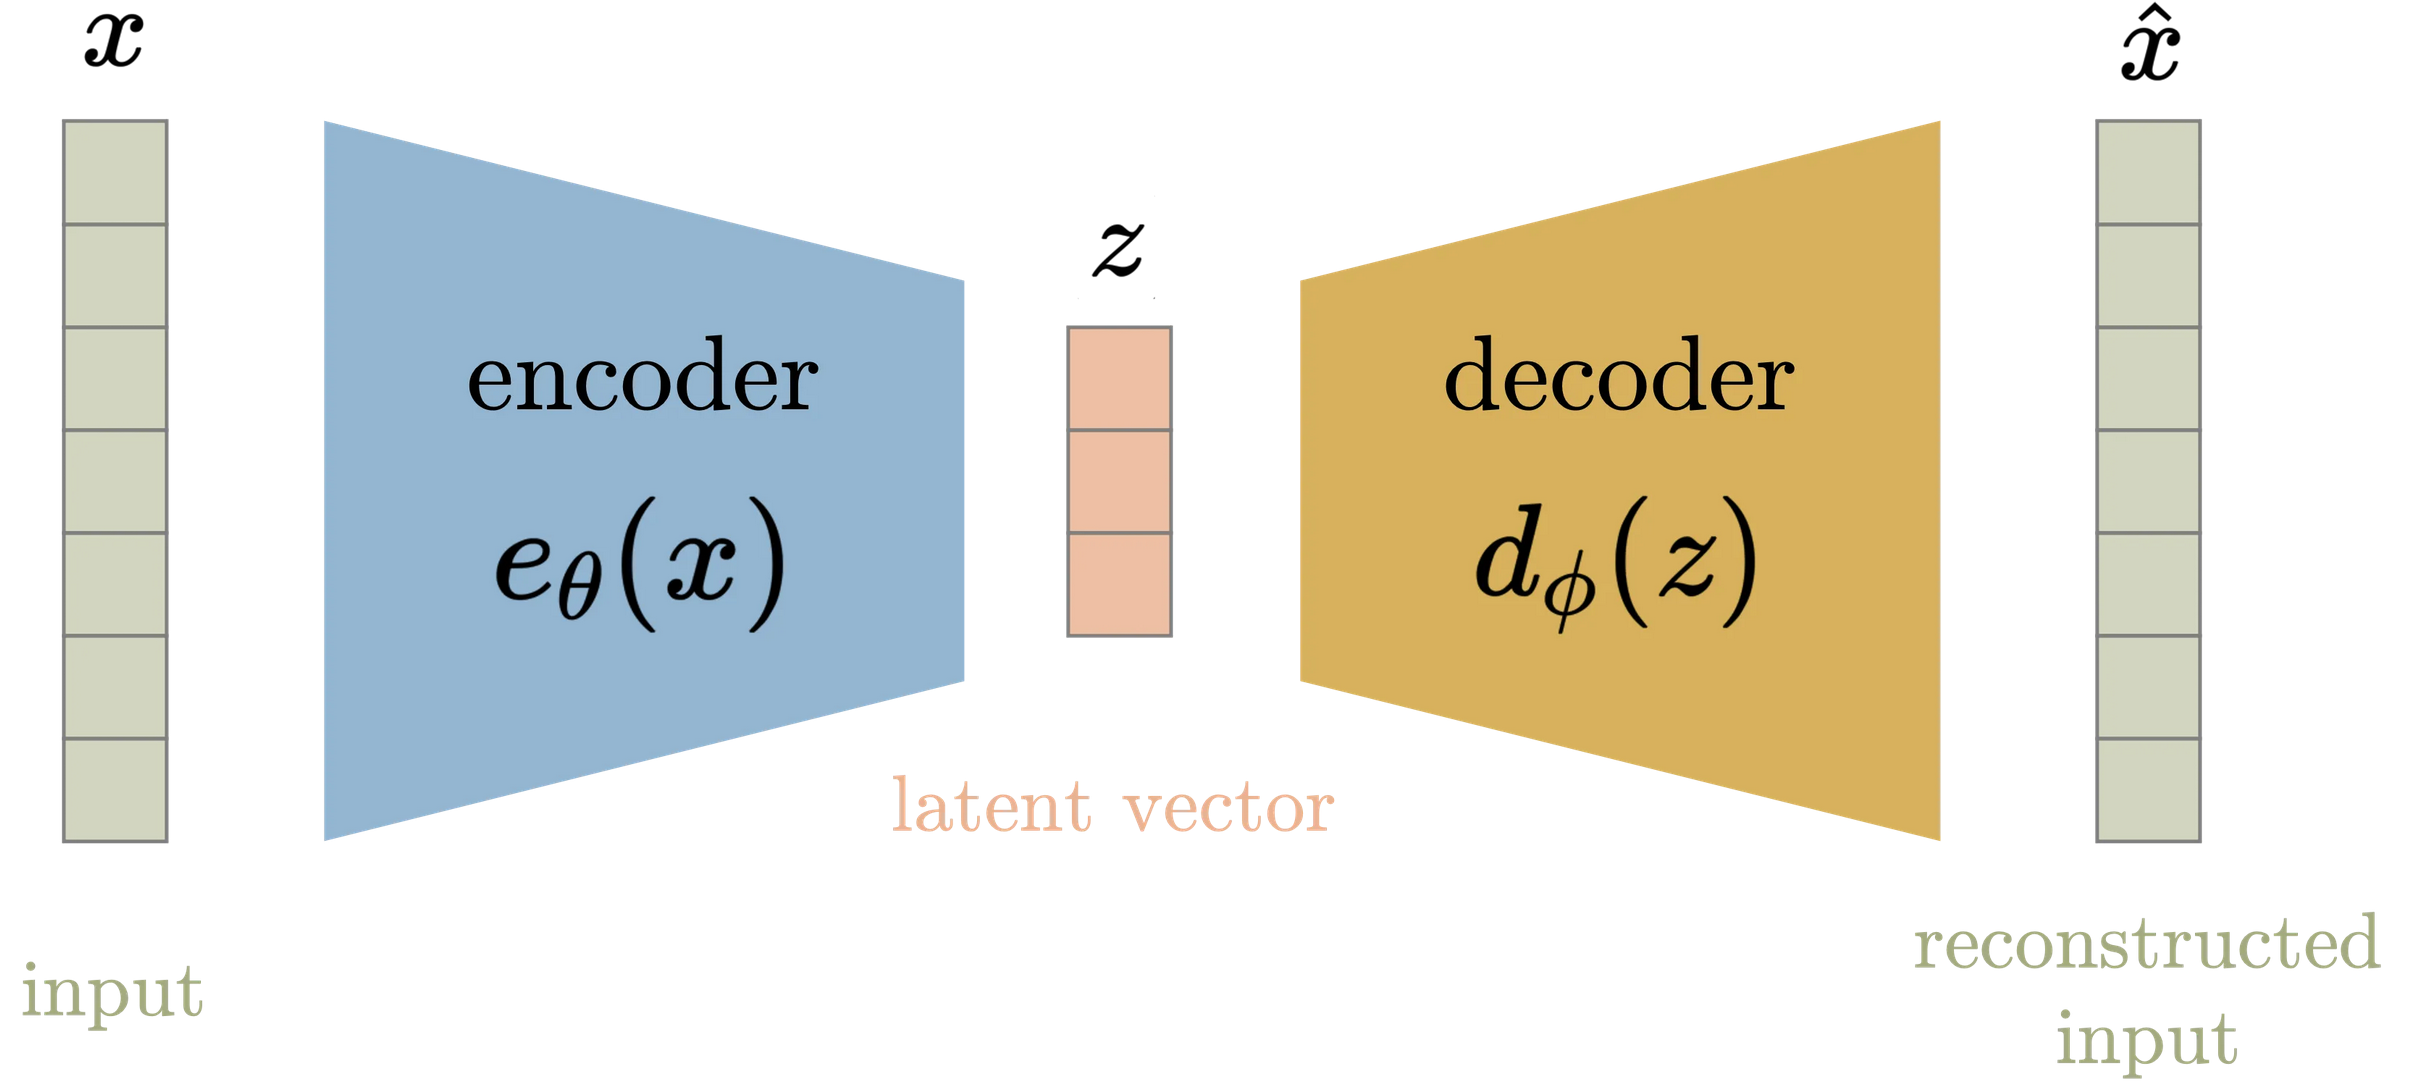
\includegraphics[scale=0.20]{pictures/ae.png}
                \caption{Skizze eines Autoencoders \cite{towards_ae_vae}.}
            \end{figure}

\newpage
            Der Autoencoder lernt die Funktion
            $e_{\theta}: \mathbb{R}^n \rightarrow \mathbb{R}^p \, \text{(Encoder)}$ und \\
            $d_{\phi} : \mathbb{R}^p \rightarrow \mathbb{R}^n \, \text{(Decoder)}$
            welche folgende Bedingung erfüllen muss.\bigskip
            \begin{center}
                $\argmin_{e_{\theta},d_{\phi}} \, \mathbb{E} \left[ \Delta \left( x, d_{\phi}(e_{\theta}(x)) \right) \right]$ \\
            \end{center}
   
            wobei $\mathbb{E}$ den Erwartungswert über die Verteilung von $x$ darstellt und $\Delta$ die Funktion für den Rekonstruktionsverlust ist,
            die die Distanz zwischen der Ausgabe des Decoders und der Eingabe misst \\
            (\emph{Dor Bank, Noam Koenigstein, Raja Giryes}, 3. Apr 2021, Paper zu Autoencoders). \\
            Anders ausgedrückt ist der Loss:
            \begin{center}
                $L(\theta, \phi) = ||x - \hat{x}||_{2}^2 = ||x - d_{\phi}(z)||_{2}^2 = ||x - d_{\phi}(e_{\theta}(x))||_{2}^2$
            \end{center}

            Während des Trainings werden die Eingabedaten $x$ in den Encoder $e_{\theta}(x)$ hineingegeben.
            Diese Funktion enkodiert die Daten durch mehrere Schichten in eine kleinere latente Dimension $z$.
            Anschließend wird $z$ dem Decoder übergeben, dessen Funktion den latenten Vektor zurück in ein $\hat{x}$ dekodiert.
            Das Modell wird mithilfe einer Verlustfunktion trainiert, die dafür sorgt, dass der sogenannte Mean Squared Error (MSE) zwischen $x$ und $\hat{x}$ so gering wie möglich wird \cite{towards_ae_vae, ae_paper}.

            \begin{figure}[!htb]
                \centering
                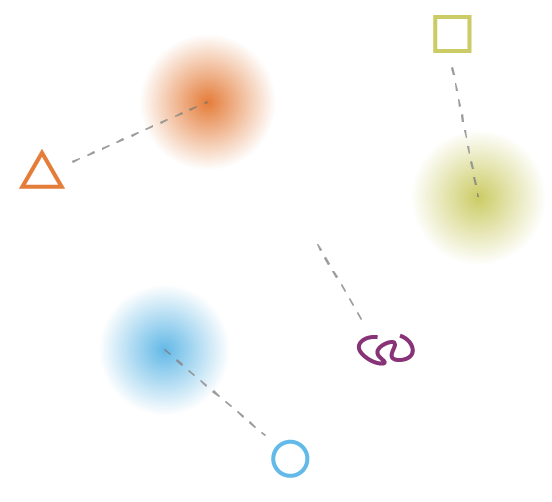
\includegraphics[scale=0.38]{pictures/Autoencoder_Latentdim.png}
                \caption{Latenter Raum eines AE \cite{towards_ae_vae, uni_hamburg}.}
            \end{figure}

            Das Problem eines Autoencoders ist, dass er lediglich die Daten komprimiert, jedoch der latente Raum eine deterministische Repräsentation liefert. Das bedeutet, dass alle Eingaben auf einen festen Punkt im latenten Raum abgebildet werden.
            Es wird keine Wahrscheinlichkeitsverteilung berücksichtigt.
            Dadurch gibt es keine Zusammenhänge zwischen ähnlichen Datenpunkten im latenten Raum.
            Der Autoencoder ist somit nicht in der Lage, neue brauchbare Daten zu generieren, sondern lediglich Eingabedaten zu rekonstruieren \cite{py_mage}.
            
\begin{comment}            
\newpage
 
\textbf{Autoencoder (AE)}
\begin{minted}[linenos, fontsize=\footnotesize, frame=lines]{python}
class Encoder(nn.Module):
    def __init__(self, width, height, latent_dim):
        super(Encoder, self).__init__()
        
        self.encoder = nn.Sequential(
            nn.Linear(height*width, 1024),
            nn.ReLU(True),
            nn.Linear(1024, 128),
            nn.ReLU(True),
            nn.Linear(128, 64),
            nn.ReLU(True),
            nn.Linear(64, latent_dim),
            nn.ReLU(True)
        )

    def forward(self, x):
        out = self.encoder(x) 
        return out

class Decoder(nn.Module):
    def __init__(self, width, height, latent_dim):
        super(Decoder, self).__init__()
        
        self.decoder = nn.Sequential(
            nn.Linear(latent_dim, 64),
            nn.ReLU(True),
            nn.Linear(64, 128),
            nn.ReLU(True),
            nn.Linear(128, 1024),
            nn.ReLU(True),
            nn.Linear(1024, height*width),
            nn.Sigmoid()
        )
        
    def forward(self, x):
        out = self.decoder(x)       
        return out

class Autoencoder(nn.Module):
    def __init__(self, width, height, latent_dim):
        super(Autoencoder, self).__init__()
        self.width = width
        self.height = height
        self.latent_dim = latent_dim
        self.encoder = Encoder(width, height, latent_dim)
        self.decoder = Decoder(width, height, latent_dim)

    def forward(self, x):   
        x = x.view(x.size(0), -1)
        out = self.encoder(x) 
        out = self.decoder(out)
        out = out.view(out.size(0), -1, self.width, self.height)  
        return out
\end{minted}

\textbf{Covolutional Autoencoder (CAE)}
\begin{minted}[linenos, fontsize=\footnotesize, frame=lines]{python}
class Encoder(nn.Module):
    def __init__(self, in_channels, latent_dim):
        super(Encoder, self).__init__()
        
        self.encoder = nn.Sequential(
            nn.Conv2d(in_channels, 1024, kernel_size=4, stride=2, padding=1),
            nn.ReLU(True),
            nn.Conv2d(1024, 128, kernel_size=4, stride=2, padding=0),
            nn.ReLU(True),
            nn.Conv2d(128, 64, kernel_size=4, stride=2, padding=1),
            nn.ReLU(True),
            nn.Conv2d(64, latent_dim, kernel_size=3, stride=1, padding=0),
            nn.ReLU(True)
        )

    def forward(self, x):
        out = self.encoder(x)    
        return out

class Decoder(nn.Module):
    def __init__(self, out_channels, latent_dim):
        super(Decoder, self).__init__()
        
        self.decoder = nn.Sequential(
            nn.ConvTranspose2d(latent_dim, 64, kernel_size=3, stride=1,
            padding=0),
            nn.ReLU(True),
            nn.ConvTranspose2d(64, 128, kernel_size=4, stride=2, padding=1),
            nn.ReLU(True),
            nn.ConvTranspose2d(128, 1024, kernel_size=4, stride=2, padding=0),
            nn.ReLU(True),
            nn.ConvTranspose2d(1024, out_channels, kernel_size=4, stride=2,
            padding=1),
            nn.Sigmoid()
        )
        
    def forward(self, x):
        out = self.decoder(x)    
        return out

class Conv_Autoencoder(nn.Module):
    def __init__(self, in_channels, out_channels, latent_dim):
        super(Conv_Autoencoder, self).__init__()
        
        self.encoder = Encoder(in_channels, latent_dim)
        self.decoder = Decoder(out_channels, latent_dim)

    def forward(self, x):
        out = self.encoder(x)        
        out = self.decoder(out)
        return out
\end{minted}
            Der Quelltext in PyTorch für zwei Autoencoder:
            Der Vorteil eines Convolutional Autoencoders (CAE) gegenüber eines Autoencoders (AE) mit linearen Schichten (Fully Connected Layers) ist, dass er bessere Ergebnisse bei der Bildverarbeitung liefert, dank seiner Convolutional Schichten.
            Ein weiterer Vorteil ist, dass er Bilder unabhängig von ihrer Größe $H \times W$ entgegennehmen kann.
            Dies ermöglicht es einem Autoencoder, der nur aus Convolutional Schichten besteht, jede beliebige Bildgröße zu verarbeiten.
\end{comment}
    
\newpage
        \subsection{Variational Autoencoder}   
            \cite{towards_ae_vae, py_mage} Wie ein Autoencoder besteht auch ein Variational Autoencoder (VAE) aus zwei Teilen:
            Einem Encoder-Teil, der den Input entgegennimmt und diesen in den latenten Raum enkodiert, sowie einem Decoder-Teil, der aus dem latenten Raum versucht, das Original wieder zu rekonstruieren.
            Allerdings erweitern VAEs die Idee von Autoencodern. Denn ein VAE lernt keine deterministischen Werte, sondern eine Verteilung der Daten. Anders als beim AE ist der latente Raum keine deterministische Repräsentation der Daten, sondern eine probabilistische Interpretation, da eine Wahrscheinlichkeitsverteilung über diesen Raum gelernt wird.
            Die Idee ist also, dass Daten im latenten Raum nicht als einzelner Punkt $z$ dargestellt werden, sondern als eine Wahrscheinlichkeitsverteilung $p(z)$.
            So lernt der VAE für die latenten Variablen eine Verteilung \cite{vae_paper_1, vae_paper_2}.
            
            Das Ziel dieser probabilistischen Interpretation ist, dass nun ähnliche Eingabedaten im Latentenraum an ähnlichen oder naheliegenden Bereichen liegen.
            Dies führt zu einer besseren Generalisierung und ermöglicht es nun nicht nur, Daten zu rekonstruieren, sondern auch, neue Daten zu generieren.

            \begin{figure}[!htb]
                \centering
                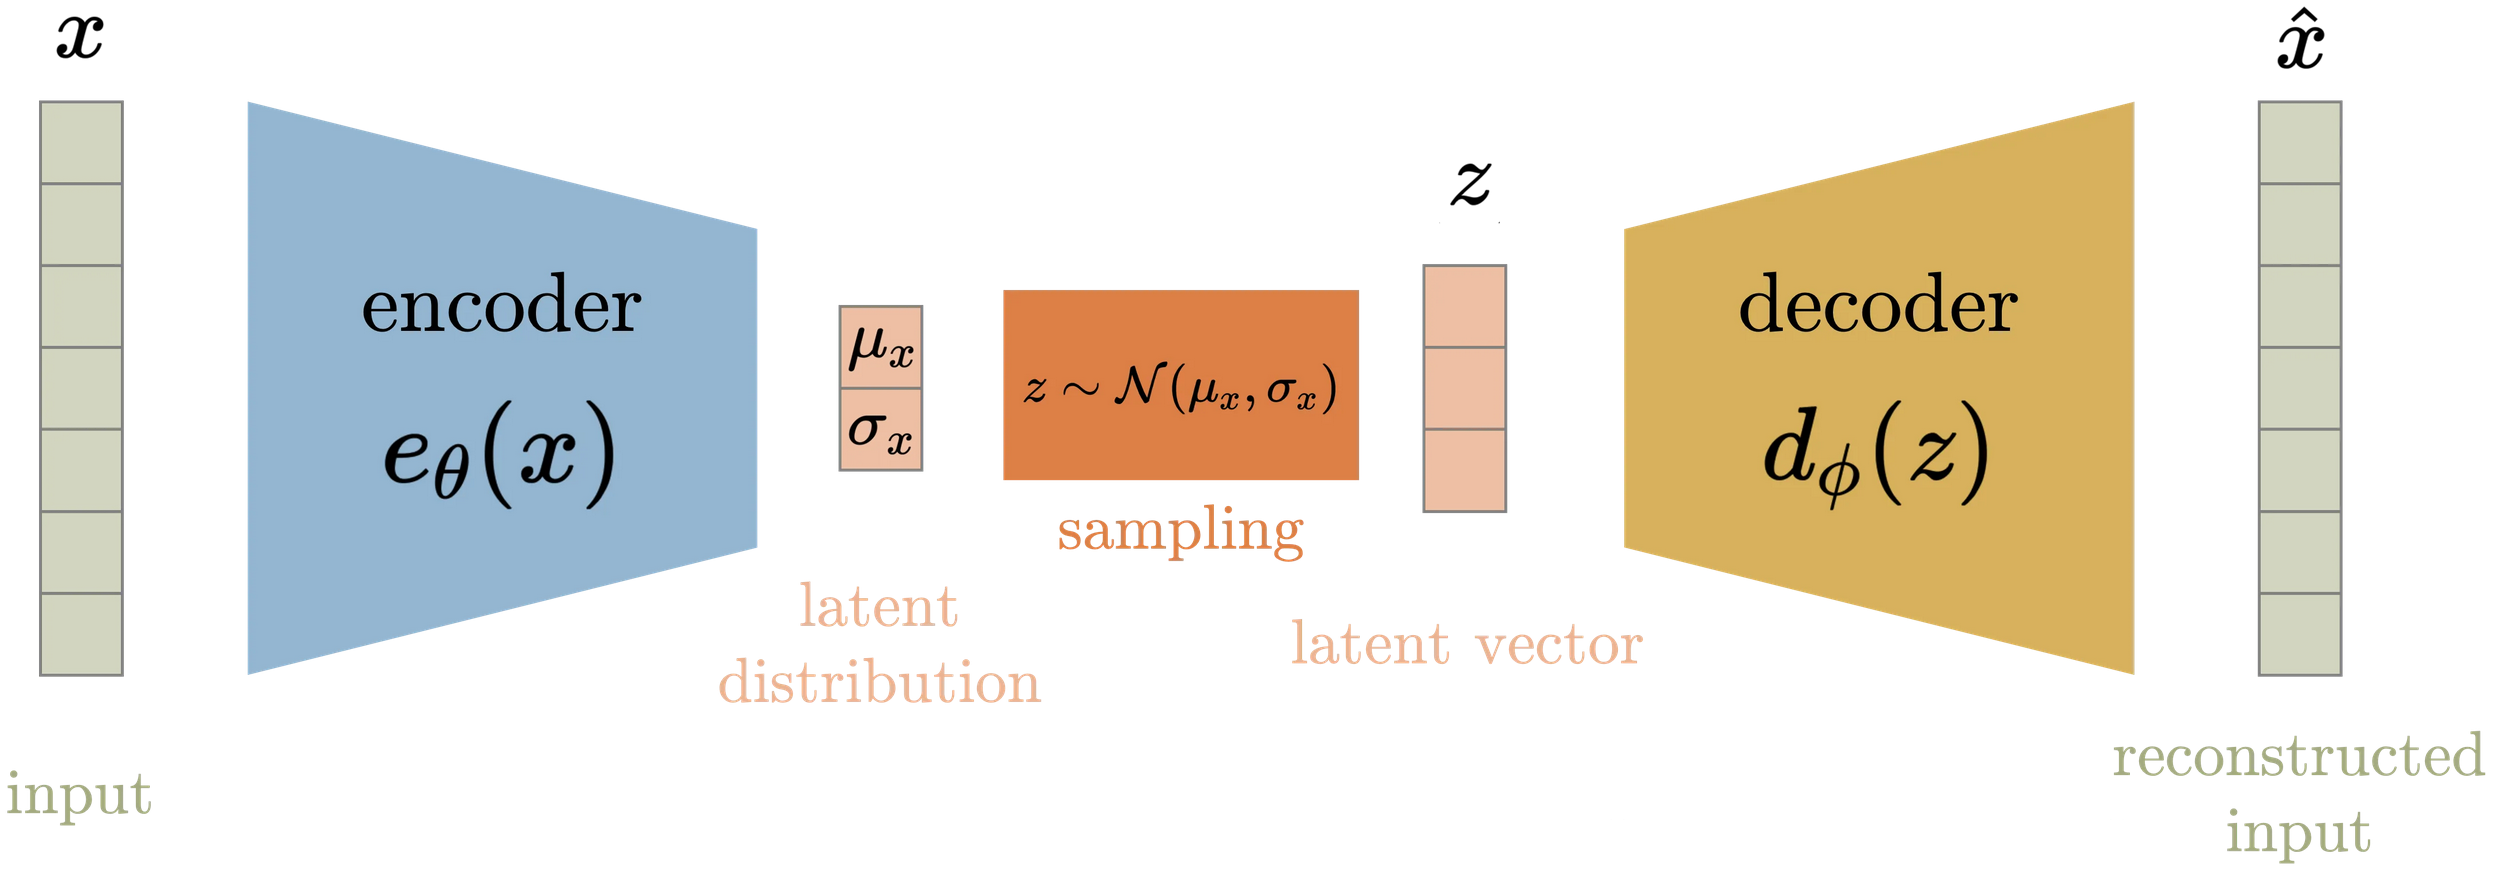
\includegraphics[scale=0.22]{pictures/vae.png}
                \caption{Skizze eines Variational Autoencoders \cite{towards_ae_vae}.}
            \end{figure}

            Ein VAE lernt also die Funktion
            $e_{\theta}: \mathbb{R}^n \rightarrow \mathbb{R}^p \, \text{(Encoder)}$ und \\
            $d_{\phi} : \mathbb{R}^p \rightarrow \mathbb{R}^n \, \text{(Decoder)}$,
            unter der Annahme, dass \bigskip

            \begin{center}
                $(\mu_{\theta}(x), \sigma_{\theta}(x)) = e_{\theta}(x)$ und $\hat{x} = d_{\phi}(z)$,\vspace{1mm}\\
                $q_\theta(z \mid x) = N(z | \mu_\theta(x), \sigma_\theta^2(x) I)$ und
                $p_\phi(\hat{x} \mid z) = N\left(\hat{x} | \mu_\phi(z), \sigma_\phi^2(z) I\right)$,\vspace{1mm}\\
                $z \sim q_\theta(z \mid x)$ und $\hat{x} \sim p_\phi(\hat{x} \mid z)$ sowie\vspace{1mm}\\
                $p(z) = N(0, I)$ und\vspace{1mm}\\
                $\argmin_{e_\theta, d_\phi} \left( \mathbb{E}[ \Delta(x, d_\phi(e_\theta(x))) ] +
                D_{KL}(q_\theta(z \mid x) \| p(z)) \right)$
            \end{center}
\newpage
            Diese Formel beschreibt die Optimierungsaufgabe eines Variational Autoencoders (VAE).
            Sie zeigt, wie die Parameter $\theta$ des Encoders sowie $\phi$ des Decoders angepasst werden, damit das Modell möglichst verlustfreie Vorhersagen treffen kann.
    
            Der VAE hat zwei Verlustfunktionen. Der Reconstruction Loss misst, wie stark sich die rekonstruierte Ausgabe von der Eingabe unterscheidet. Des Weiteren gibt es die KL-Divergenz (Kullback-Leibler-Divergenz), die den Unterschied zwischen der latenten Verteilung $q_\theta(z \mid x)$ und der gewünschten Verteilung $p(z)$, also der Normalverteilung, misst. Das Ziel ist es, den regularisierten Raum so nah wie möglich an die Normalverteilung zu bringen \cite{towards_ae_vae, vae_paper_1, vae_paper_2}.\bigskip
            \begin{center}
                $reconstruction \ loss = \| x - d_\phi(\mu_\theta(x) + \sigma_\theta(x) \cdot \epsilon) \|_2^2$\vspace{1mm}\\
                $KL-Divergenz = D_{KL}(q_\theta(z \mid x) \| p(z))$\vspace{1mm}\\
                $L(\theta, \phi) = \| x - d_\phi(\mu_\theta(x) + \sigma_\theta(x) \cdot \epsilon) \|_2^2 +
                D_{KL}(q_\theta(z \mid x) \| p(z))$
            \end{center}
            \bigskip

            Die folgenden Schritte zeigen den Ablauf eines VAE:
            \begin{enumerate}
                \item Input\\
                    Der Encoder nimmt die Eingabedaten entgegen, die kodiert werden sollen.
                \item Mittelwert und Standartabweichung\\
                    Der Encoder erzeugt eine latente Distribution bestehend aus Standartabweichung $\sigma$ und Mittelwert $\mu$.
                \item Sampling\\
                    Um $z$ zu berechnen wird ein zufälliger Datenpunkt $\epsilon$ aus der Normalverteilung $q_\theta(z \mid x)$ gewählt.\\
                    $z = \mu_\theta(x) + \sigma_\theta(x) \cdot \epsilon$
                \item Rekonstruktion\\
                    $z$ wird dann dem Decoder übergeben welcher lernt aus der Wahrscheinlichkeitsverteilung das Bild erneut zu Rekonstruieren. 
            \end{enumerate}
\newpage   
            Da im Gegensatz zu einem AE der latente Raum nun auf einer Normalverteilung beruht, sind bei einem VAE ähnliche Daten in Clustern zusammengefasst. Dies ermöglicht es, mit einem VAE sinnvolle Daten zu generieren.
    
            \begin{figure}[!htb]
                \centering
                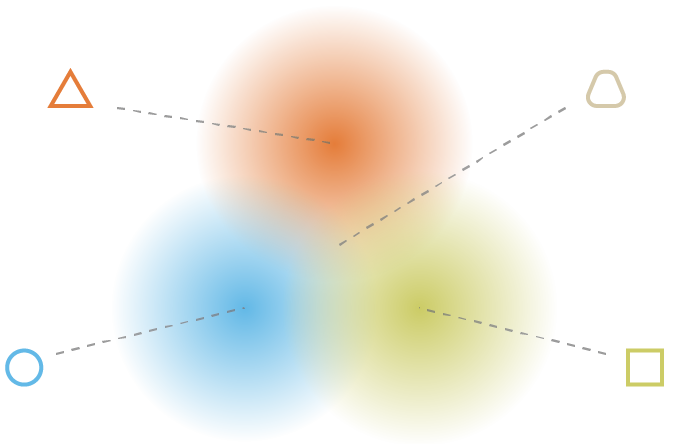
\includegraphics[scale=0.35]{pictures/VAE_Latentdim.png}
                \caption{Latenter Raum eines VAE \cite{towards_ae_vae, uni_hamburg}.}
            \end{figure}

            \begin{figure}[!htb]
                \centering
                
\includegraphics[scale=0.32]{pictures/mnist latent dim.png}
                \caption{Latenter Raum eines VAE dargestellt mit dem MNIST-Datensatz \cite{vae_keras}.}
            \end{figure}

\begin{comment}
\newpage
\textbf{Variational Autoencoder (VAE)}
\begin{minted}[linenos, fontsize=\footnotesize, frame=lines]{python}
class Encoder(nn.Module):
    def __init__(self, in_channels, latent_dim):
        super(Encoder, self).__init__()
        
        self.encoder = nn.Sequential(
            nn.Conv2d(in_channels, 1024, kernel_size=4, stride=2, padding=1),
            nn.ReLU(True),
            nn.Conv2d(1024, 128, kernel_size=4, stride=2, padding=0),
            nn.ReLU(True),
            nn.Conv2d(128, 64, kernel_size=4, stride=2, padding=1),
            nn.ReLU(True)
        )

        self.conv_mu = nn.Conv2d(64, latent_dim, kernel_size=3, stride=1, padding=0)
        self.conv_logvar = nn.Conv2d(64, latent_dim, kernel_size=3, stride=1, padding=0)

    def forward(self, x):
        out = self.encoder(x)
        mu = self.conv_mu(out)
        logvar = self.conv_logvar(out)
        return mu, logvar

class Decoder(nn.Module):
    def __init__(self, out_channels, latent_dim):
        super(Decoder, self).__init__()
        
        self.decoder = nn.Sequential(
            nn.ConvTranspose2d(latent_dim, 64, kernel_size=3, stride=1, padding=0),
            nn.ReLU(True),
            nn.ConvTranspose2d(64, 128, kernel_size=4, stride=2, padding=1),
            nn.ReLU(True),
            nn.ConvTranspose2d(128, 1024, kernel_size=4, stride=2, padding=0),
            nn.ReLU(True),
            nn.ConvTranspose2d(1024, out_channels, kernel_size=4, stride=2, padding=1),
            nn.Sigmoid()
        )
        
    def forward(self, x):
        out = self.decoder(x)    
        return out

class VAE(nn.Module):
    def __init__(self, in_channels, out_channels, latent_dim):
        super(VAE, self).__init__()
        
        self.encoder = Encoder(in_channels, latent_dim)
        self.decoder = Decoder(out_channels, latent_dim)

    def reparameterize(self, mu, logvar):
        std = torch.exp(0.5 * logvar)
        eps = torch.randn_like(std).to(DEVICE)
        return mu + eps * std

    def forward(self, x):
        mu, logvar = self.encoder(x)
        z = self.reparameterize(mu, logvar)
        x_hat = self.decoder(z)
        return x_hat, mu, logvar
\end{minted}
\end{comment}

\newpage
        \subsection{Vector Quantized Variational Autoencoder}
            \begin{figure}[!htb]
                \centering
                \includegraphics[scale=0.5]{pictures/catdog.png}
                \caption{Comic Figur Catdog aus der Serie Catdog \cite{catdog, cat, dog}.}
            \end{figure}
    
            Wie in \cite{vqvae_paper, vqvae_super, vqvae} beschrieben, ist ein Vektor Quantized Variational Autoencoder (VQ-VAE) eine Erweiterung des klassischen VAE. Während ein VAE die Daten in eine stetige Repräsentation des latenten Raums überführt, wird bei einem VQ-VAE die latente Repräsentation der Daten diskret. Die Motivation hinter dieser Diskretisierung liegt darin, dass wir in einer diskreten Welt leben. Es gibt keine Zwischenzustände wie „halb Mensch, halb Baum“ oder „halb Hund, halb Katze“. Ein VQ-VAE zielt darauf ab, die Daten auf eine diskrete Weise zu quantisieren.

            Wie alle anderen Autoencoder-Modelle besteht auch ein VQ-VAE aus einem Encoder und einem Decoder. In der Mitte befindet sich zusätzlich ein Quantifizierer und ein sogenanntes Codebook. Das Codebook ist eine Lookup-Tabelle, in der sogenannte Embedding-Vektoren gespeichert sind.
            Der Encoder kodiert die Eingabedaten zu einem latenten Vektor der Dimension $D$, der einen Datenpunkt im latenten Raum repräsentiert. Im Quantifizierungsschritt wird im Codebook nach dem nächstliegenden Embedding-Vektor (Codebook-Vektor)  gesucht und ersetzt den latenten Vektor durch diesen. Anschließend wird der neue latente Vektor, welcher ersetzt wurde, durch den Decoder wieder rekonstruiert.
            Die Embedding-Vektoren im Codebook müssen dabei die gleiche Dimension $D$ wie der latente Vektor haben.
    
\newpage
            \begin{figure}[!htb]
                \centering
                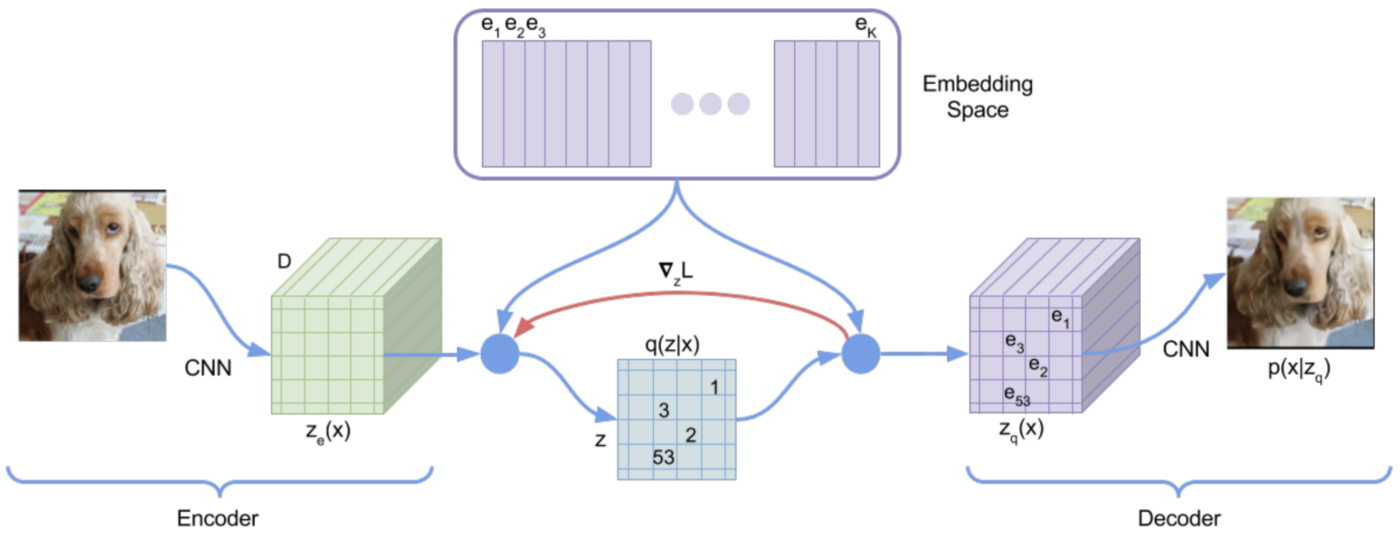
\includegraphics[scale=0.29]{pictures/vq-vae.png}
                \caption{Architektur eines VQ-VAE mit Straight-through estimation \cite{vqvae_pic}.}
            \end{figure}

            Ein VQ-VAE lernt die Funktion\\
            $e_{\theta}: \mathbb{R}^n \rightarrow \mathbb{R}^D_z \, \text{(Encoder)}$,
            $\mathbb{R}^D_z \rightarrow \mathbb{R}^D_q \text{(Quantifizierer)}$ und
            $d_{\phi} : \mathbb{R}^D_q \rightarrow \mathbb{R}^n \, \text{(Decoder)}$.
            \bigskip

            \begin{center}
                Der latente Raum ist definiert als $z_e(x) = e_\theta(x)$.\\
                Der Embedding-Space ist definiert als $e \in \mathbb{R}^{K \times D}$. \\
                $e_i \in \mathbb{R}^D, \; i \in \{1, 2, \dots, K\}$\\
                $K = Anzahl \ Codebook \ Vektoren$ und\\
                $D = Dimension \ jedes \ Latenten \ und \ Embedding \ Vektors$.\\
            \end{center}
            \begin{center}
                $q(z = e_k \mid x) = 
                \begin{cases} 
                1 & \text{für } k = \arg\min_j \| z_e(x) - e_j \|_2^2, \\
                0 & \text{sonst}
                \end{cases}$\\
                $z_q(x) = e_k, \; \text{wobei } k = \arg\min_j \| z_e(x) - e_j \|_2^2$
            \end{center}

            Für den latenten Vektor $z_e$ wird nach dem passenden Embedding-Vektor im Codebook gesucht $e_i$,
            der den geringsten Abstand zu $z_e$ hat. Dies geschieht durch Minimierung mit $\arg\min$.
            Der latente Vektor $z_e$ wird dann ersetzt $q(e_k \mid x)$, sodass
            $z_q(x) = e _k$.

            Der Embedding-Vektor $z_q(x)$ wird anschließend vom Decoder dekodiert, der das rekonstruierte Ausgabebild generiert \cite{vqvae_paper}.
    
\newpage
            \cite{vqvae} Die Verlustfunktion eines VQ-VAE setzt sich aus drei Hauptkomponenten zusammen:
            \begin{enumerate}
                \item Reconstruction Loss\\
                    Der Reconstruction Loss misst, wie auch bei den Autoencodern zuvor, den Unterschied zwischen dem Eingabebild und dem rekonstruierten Ausgang. Die Differenz zwischen den beiden Bildern ergibt den Reconstruction Loss.\\
                    $L_{\text{recon}} = \| x - \hat{x} \|_2^2$
                \item Codebook Loss\\
                    Dieser misst den Loss des Codebooks, d.h. den Abstand zwischen dem latenten Vektor
                    $z_e(x)$ dem nächstgelegenen Embedded Vektor $e_k$. Der Operator sg (Stop Gradient) verhindert, dass dieser Term den Encoder während des Trainings beeinflusst. Es soll lediglich das Codebook aktualisiert werden.\\
                    $L_{\text{codebook}} = \| \operatorname{sg}[z_e(x)] - e_k \|_2^2$\\
                \item Commitment Loss\\
                    Dieser Term sorgt dafür, dass der Encoder im Einklang mit dem Quantifizierungsschritt bleibt und stellt sicher, dass die Ausgaben des Encoders, also die latenten Vektoren, sich in Richtung des nächstgelegenen Embedding-Vektors bewegen. $\beta$ reguliert die stärke des Verlustes.\\
                    $L_{\text{commit}} = \beta \| z_e(x) - \operatorname{sg}[e_k] \|_2^2$\\
            \end{enumerate}
            \begin{center}
                $L_{\text{total}} = L_{\text{recon}} + L_{\text{codebook}} + L_{\text{commit}}$\\
                $L(\theta, \phi, x, e) = \| x - \hat{x} \|_2^2 + \| \operatorname{sg}[z_e(x)] - e_k \|_2^2 + \beta \| z_e(x) - \operatorname{sg}[e_k] \|_2^2$
            \end{center} 
\begin{comment}
\newpage
\textbf{Vector Quantized Variational Autoencoder (VQ-VAE)}
\begin{minted}[linenos, fontsize=\footnotesize, frame=lines]{python}
 class Encoder(nn.Module):
    def __init__(self, in_channels, embedding_dim):
        super(Encoder, self).__init__()
        self.encoder = nn.Sequential(
            nn.Conv2d(in_channels, 1024, kernel_size=4, stride=2, padding=1),
            nn.ReLU(True),
            nn.Conv2d(1024, 128, kernel_size=4, stride=2, padding=0),
            nn.ReLU(True),
            nn.Conv2d(128, 64, kernel_size=4, stride=2, padding=1),
            nn.ReLU(True),
            nn.Conv2d(64, embedding_dim, kernel_size=4, stride=2, padding=1),
            nn.ReLU(True)
        )

    def forward(self, x):
        return self.encoder(x)  

class Decoder(nn.Module):
    def __init__(self, out_channels, embedding_dim):
        super(Decoder, self).__init__()
        self.decoder = nn.Sequential(
            nn.ConvTranspose2d(embedding_dim, 64, kernel_size=3, stride=1, padding=0),
            nn.ReLU(True),
            nn.ConvTranspose2d(64, 128, kernel_size=4, stride=2, padding=1),
            nn.ReLU(True),
            nn.ConvTranspose2d(128, 1024, kernel_size=4, stride=2, padding=0),
            nn.ReLU(True),
            nn.ConvTranspose2d(1024, out_channels, kernel_size=4, stride=2, padding=1),
            nn.Sigmoid()
        )

    def forward(self, x):
        return self.decoder(x)

class VectorQuantizer(nn.Module):
    def __init__(self, num_embeddings, embedding_dim, commitment_cost=0.25):
        super(VectorQuantizer, self).__init__()
        
        self._embedding_dim = embedding_dim
        self._num_embeddings = num_embeddings
        
        self._embedding = nn.Embedding(self._num_embeddings, self._embedding_dim)
        self._embedding.weight.data.uniform_(-1/self._num_embeddings, 1/self._num_embeddings)
        self._commitment_cost = commitment_cost

    def forward(self, inputs):
        inputs = inputs.permute(0, 2, 3, 1).contiguous()
        input_shape = inputs.shape
        
        flat_input = inputs.view(-1, self._embedding_dim)
        
        distances = (torch.sum(flat_input**2, dim=1, keepdim=True) 
                    + torch.sum(self._embedding.weight**2, dim=1)
                    - 2 * torch.matmul(flat_input, self._embedding.weight.t()))
            
        encoding_indices = torch.argmin(distances, dim=1).unsqueeze(1)
        encodings = torch.zeros(encoding_indices.shape[0], self._num_embeddings, device=inputs.device)
        encodings.scatter_(1, encoding_indices, 1)
        
        quantized = torch.matmul(encodings, self._embedding.weight).view(input_shape)
        
        e_latent_loss = F.mse_loss(quantized.detach(), inputs)
        q_latent_loss = F.mse_loss(quantized, inputs.detach())
        loss = q_latent_loss + self._commitment_cost * e_latent_loss
        
        quantized = inputs + (quantized - inputs).detach()
        avg_probs = torch.mean(encodings, dim=0)
        perplexity = torch.exp(-torch.sum(avg_probs * torch.log(avg_probs + 1e-10)))
        
        return quantized.permute(0, 3, 1, 2).contiguous(), loss, perplexity, encodings

class VQVAE(nn.Module):
    def __init__(self, in_channels, out_channels, num_embeddings, embedding_dim):
        super(VQVAE, self).__init__()
        self.encoder = Encoder(in_channels, embedding_dim)
        self.decoder = Decoder(out_channels, embedding_dim)
        self.vq_layer = VectorQuantizer(num_embeddings, embedding_dim)

    def forward(self, x):
        z_e = self.encoder(x)
        quantized, vq_loss, perplexity, _ = self.vq_layer(z_e)
        x_recon = self.decoder(quantized)
        return x_recon, vq_loss, perplexity

\end{minted}
\end{comment}

\newpage
\section{Metriken}
    \subsection{Mean Squared Error}
            Der Mean Squared Error (MSE) ist eine gängige Metrik zum Messen von Vorhersagen oder Rekonstruktionen.
            Er misst die durchschnittliche quadratische Differenz der tatsächlichen/originalen Daten und der vorhergesagten/rekonstruierten Daten.
            Ein niedriger MSE deutet darauf hin, dass das rekonstruierte oder vorhergesagte $\hat{x}$ nahe am Original $x$ liegt.\bigskip
            \begin{center}
                $\text{MSE} = \frac{1}{n} \sum_{i=1}^{n} (x_i - \hat{x}_i)^2$
            \end{center}

            \begin{enumerate}
                \item Vorteile
                \begin{itemize}
                    \item Große Fehler werden durch das Quadrieren stärker bestraft. Dies ist von Vorteil, wenn große Fehler minimiert werden sollen \cite{mse_builtin}.
                    \item Der MSE ist zudem mathematisch einfach zu berechnen.
                \end{itemize}
                \item Nachteile
                \begin{itemize}
                    \item Der MSE ist empfindlich gegenüber Ausreißern. Er bestraft große Fehler (Ausreißer) unverhältnismäßig stark, da die Fehler quadriert werden. Ein einziger großer Fehler kann den gesamten MSE-Wert erheblich erhöhen, selbst wenn die meisten anderen Fehler gering sind \cite{mse_builtin}.
                    \item             
                    Sowohl der MSE als auch der PSNR sind Metriken, die sich ohne hohen Aufwand
                    implementieren und berechnen lassen. Sie haben jedoch einige Einschränkungen: Der
                    MSE berücksichtigt nicht die Wahrnehmung des menschlichen Auges und kann daher
                    Unterschiede in der visuellen Qualität nicht immer genau erfassen \cite{mse_psnr_eye}.
                \end{itemize}
            \end{enumerate}

\newpage
        \subsection{Peak Signal-to-Noise Ratio}
            Die Peak Signal-to-Noise Ratio (PSNR) ist eine Metrik, mit der sich die Qualität eines rekonstruierten oder komprimierten Bildes im Vergleich zum Original ermitteln lässt.
            Die PSNR misst den sogenannten Rauschpegel zwischen dem Originalbild und dem rekonstruierten Bild.
            Ein hoher PSNR-Wert deutet auf eine bessere Qualität hin, da das Rauschen bzw. die Differenz zum Original geringer ist \cite{psnr, psnr2}.
            \begin{center}
                $\text{PSNR} = 10 \cdot \log_{10} \left( \frac{\text{MAX}^2}{\text{MSE}} \right)$
            \end{center}
            \begin{enumerate}
                \item Vorteile
                \begin{itemize}
                    \item Einheitliche Skala in Dezibel lässt sich gut interpretieren \cite{psnr3}.
                    \item Sowie beim MSE hat die PSNR eine starke Gewichtung auf große Fehler.
                \end{itemize}
                \item Nachteile
                \begin{itemize}
                    \item Da PSNR ebenfalls auf dem MSE basiert, erbt er dessen Empfindlichkeit gegenüber Ausreißern, sowie andere Nachteile wie das die PSNR nicht die Menschliche Wahrnehmung berücksichtigt.
                    \item Die PSNR berücksichtigt nicht, wie Menschen Bilder wahrnehmen. Kleinere Details oder Farbabweichungen, die für das menschliche Auge vielleicht weniger auffällig sind, werden im PSNR-Wert genauso stark gewichtet wie wichtige Bilddetails \cite{mse_psnr_eye}.
                \end{itemize}
            \end{enumerate}

\newpage
        \subsection{Structural Similarity Index}
            \cite{ssim_paper}
            Der Structural Similarity Index (SSIM) ist eine weitere Metrik zur Messung der Bildqualität. Im Gegensatz zu PSNR und MSE berücksichtigt SSIM die Wahrnehmung des menschlichen Auges.
            Bilder werden hinsichtlich ihrer Struktur, Helligkeit und Kontrast bewertet.
            
            \begin{center}    
                Die \textbf{Helligkeit $(l)$} \vspace{1mm} lässt sich berechnen durch \\
                $l(x, y) = \frac{2 \mu_x \mu_y + C_1}{\mu_x^2 + \mu_y^2 + C_1}$ \vspace{1mm}\\
                wo $\mu_x$ und $\mu_y$ die Mittelwerte der Pixelintensität von $x$ und $y$ sind.\\
                $C_1 = (K_1 \cdot L)^2$ zur vermeidung von Störungen, $K_1 \approx 0.01$ und
                $L = \max(p), \quad p \in (0, 255) \max$.\\
            \end{center}
            \begin{center}    
                Der \textbf{Kontrast $(c)$} \vspace{1mm} lässt sich berechnen durch \\
                $c(x, y) = \frac{2 \sigma_x \sigma_y + C_2}{\sigma_x^2 + \sigma_y^2 + C_2}$ \vspace{1mm}\\
                $\sigma_x$ und $\sigma_y$ sind die Standardabweichungen der Pixelintensität von $x$ und $y$.\\
                $C_2 = (K_2 \cdot L)^2 \quad \text{mit} \quad K_2 \approx 0.03$
            \end{center}
            \begin{center}    
                Die \textbf{Struktur  $(s)$} \vspace{1mm} lässt sich berechnen durch \\
                $s(x, y) = \frac{\sigma_{xy} + C_3}{\sigma_x \sigma_y + C_3}$ \vspace{1mm}\\
                $\sigma_{xy}$ ist die Kovarianz zwischen $x$ und $y$.\\
                $C_3 = (C_2 / 2)$
            \end{center}
            
            \begin{center}    
                $\text{SSIM}(x, y) = [l(x, y)]^\alpha \cdot [c(x, y)]^\beta \cdot [s(x, y)]^\gamma$
            \end{center}
       
            \begin{enumerate}
                \item Vorteile
                \begin{itemize}
                    \item Die Berücksichtigung der menschlichen Wahrnehmung ist beim SSIM gegeben. SSIM wurde entwickelt, um die wahrgenommene Bildqualität besser durch Helligkeit, Struktur und Kontrast erfassen zu können 
                    \cite{wikipedia_ssim}.
                    \item Studien haben ergeben, dass der SSIM eine höhere Korrelation mit der subjektiven menschlichen Wahrnehmung der Bildqualität aufweist als beispielsweise die PSNR Metrik \cite{wikipedia_ssim}.
                \end{itemize}
                \item Nachteile
                \begin{itemize}
                    \item Die Berechnung des SSIM ist wesentlich Komplexer und erfordert mehr Rechenleistung.
                \end{itemize}
            \end{enumerate}    

\newpage
    \subsection{Precision}
            Precision (Präzision) ist eine Kennzahl aus der Klassifikationsbewertung.
            Die Vorhersagen des Modells sollten möglichst präzise sein. Je näher die Precision eines Modells an einem Wert von $1,0$ liegt, desto besser.
            Wenn ein Modell einen Wert \text{„1“} vorhersagt, dann sollte auch wirklich der Wert eine \text{„1“} sein.
            Dies wird mit der Precision gemessen.\newline
            \begin{center}  
                \large$prescicion = \frac{\text{true positives}}{\text{true positives} + \text{false positives}}$\\
            \end{center}
            Bedeutung:\\
            Wie viel Prozent der vorhergesagten positiven Fälle (\text{„1“}) sind auch in Wahrheit tatsächlich positiv?
            \bigskip
            
        \subsection{Recall}
            Vorhersagen sollen eine hohe Trefferquote haben. Das heißt, dass das Modell alle \text{„1“} Fälle in  den Ground-Truth-Daten
            auch als solche erkennt. Hierfür wird die Metrik Recall (Empfindlichkeit) verwendet.\newline
            \begin{center}  
                \large$recall = \frac{\text{true positives}}{\text{true positives} + \text{false negatives}}$\\
            \end{center}
            Bedeutung:\\
            Wie viel Prozent der tatsächlichen positiven Fälle (\text{„1“}) erkennt das Modell?
            \bigskip    
        \subsection{F1-Score}
            Der F1-Score sagt aus, wie gut ein Modell eine hohe Trefferquote hat, jedoch auch gleichzeitig, wie präzise es
            ist. Vorhersagen sollen sowohl eine hohe Trefferquote haben als auch präzise sein.\newline
            \begin{center} 
                \large$F1 = 2 * \frac{\text{precission} * \text{recall}}{\text{precission} + \text{recall}}$\\
            \end{center}
            
\newpage
    \subsection{Intersection over Union}
        \cite{iou, iou_paper, iou_2} Der Intersection over Union (IoU) wird zur Bewertung der Leistung von Objekterkennungsmodellen verwendet, indem die vorhergesagte Boundingbox (Begrenzungsbox) mit der tatsächlichen (Ground-Truth-Boundingbox) verglichen wird.
        Der IoU ist eine Metrik, mit der jeder Algorithmus bewertet werden kann, der vorhergesagte Boundingboxen als Ausgabe liefert.

        Um IoU zur Bewertung eines beliebigen Objekterkennungsmodells anzuwenden, benötigt man:

        \begin{itemize}
            \item Die Ground-Truth-Boundingboxen sind markierte Boundingboxen aus dem Originaldatensatz (Labeldatensatz), die die genaue Position des Objekts im Bild angeben.
            \item Die Boundingboxen, die vom Modell vorhergesagt werden.
        \end{itemize}
        Solange diese beiden Sätze von Boundingboxen vorliegen, lässt sich der IoU messen.

        \begin{figure}[!htb]
            \centering
            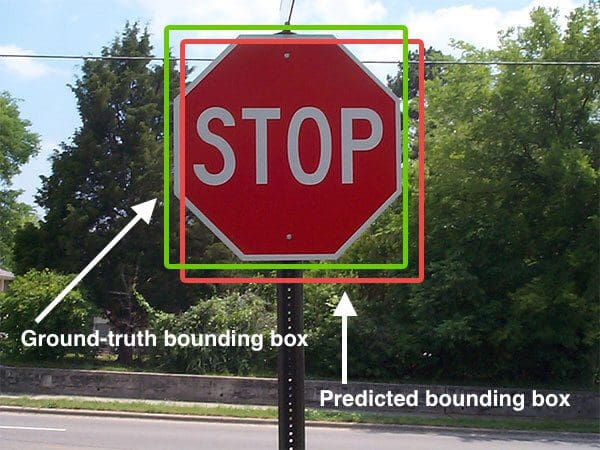
\includegraphics[scale=0.49]{pictures/iou_stop_sign.jpg}
            \caption{Die vorhergesagte Boundingbox wird in Rot dargestellt, während die Ground-Truth-Boundingbox in Grün dargestellt wird \cite{iou}.}
        \end{figure}

\newpage
        \cite{iou}
        Der IoU zwischen der vorhergesagten Boundingbox und der Ground-Truth-Boundingbox lässt sich einfach berechnen:
        Die Fläche der Schnittmenge wird durch die Fläche der Vereinigung der beiden Boundingboxen dividiert.
        
        \begin{center}  
            $Area = x2 y2 - x1 y1$\\
            wobei $x1y1$ obere linke Ecke und $x2y2$ untere rechte Ecke\\ \bigskip
            \large$IoU = \frac{Area_{Ground-Truth} \cap Area_{predicted}}{Area_{Ground-Truth} \cup Area_{predicted}}$
        \end{center}

        \begin{figure}[!htb]
            \centering
            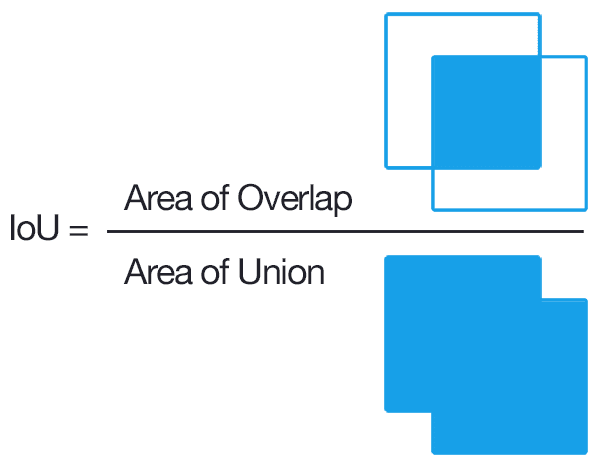
\includegraphics[scale=0.49]{pictures/iou_equation.png}
            \caption{Berechnung des IoU als Grafik \cite{iou}}.
        \end{figure}

        Bei der Verwendung von IoU als Bewertungsmetrik muss ein Schwellenwert (Threshold) für die Genauigkeit festgelegt werden, der in der Regel bei 0,5 liegt. Werte darüber werden als gut bewertet, während Werte darunter als unbrauchbar gelten \cite{iou_paper, iou_2}.

\chapter{Related Work}
    \section{Visual Recognition Models}
        \cite{visual_recognition_models_paper} In der Arbeit „Are Visual Recognition Models Robust to Image Compression?“ wird untersucht, 
        wie sich verschiedene Bildkompressionsmethoden wie JPEG auf die Leistung von visuellen Erkennungsmodellen auswirken. Dabei liegt der Fokus darauf, die Robustheit von Modellen zu analysieren, die für Aufgaben wie Bildklassifikation, Objekterkennung und Bildsegmentierung verwendet werden.

        Das Ziel der Studie ist es, zu bewerten, wie empfindlich Modelle auf die Kompression von Eingabebildern reagieren, und zu untersuchen, ob durch Anpassungen, wie beispielsweise die Feinabstimmung auf komprimierte Daten, die Auswirkungen der Kompression gemildert werden können.\\

        \underline{Erkenntnisse dieser Studie:}
        \begin{enumerate}
            \item Auswirkungen der Kompression
            \begin{itemize}
                \item Eine zu starke Kompression führt zu einem signifikanten Rückgang der Modellleistung.
                \item Verschiedene Modelle reagieren unterschiedlich empfindlich auf die Art und Stärke der Kompression.
            \end{itemize}
            \item Modellanpassung
            \begin{itemize}
                \item Modelle wie z.B. ResNet oder Vision Transformers schneiden oft besser ab als einfache Modell Architekturen.
                \item Die Feinabstimmung (Fine-Tuning) von Modellen auf komprimierte Bilder kann die Leistung wieder verbessern.
            \end{itemize}
            \item Relevanz
            \begin{itemize}
                \item In Echtzeitanwendungen wie autonomen Fahrzeugen oder\\
                Überwachungssystemen könnte die Optimierung von Modellen für komprimierte Daten dazu beitragen, die Bandbreite zu reduzieren, ohne die Systemleistung wesentlich zu beeinträchtigen.
            \end{itemize}
        \end{enumerate}      

\newpage
    \section{Learned Image Compression}
        \cite{image_compression_paper} Die Arbeit „Learned Image Compression for Machine Perception“ untersucht die Entwicklung und Anwendung von lernbasierten Bildkompressionsmethoden, die speziell auf die Anforderungen maschineller Wahrnehmung\\
        ausgerichtet sind, insbesondere im Kontext von Computer Vision und maschinellen Lernmodellen. Anstatt traditionelle Bildkompressionsmethoden wie JPEG oder PNG zu verwenden, die für die menschliche Wahrnehmung optimiert sind, wird hier ein Ansatz verfolgt, der die Kompression so gestaltet, dass sie sowohl für Menschen als auch für Maschinen, wie z. B. Objekterkennungsmodelle, effektiv ist.

        Ziel der Studie ist es, zu zeigen, dass speziell für maschinelle Wahrnehmung\\
        optimierte Bildkompressionsmethoden zu einer besseren Leistung in\\
        Visual-Recognition-Aufgaben führen können.\\
        Auch die Bildkompression sollte an ML-Modelle angepasst werden, um gleichzeitig die Nutzung zu optimieren und um genauere Modellvorhersagen zu erhalten.\\

        \underline{Erkenntnisse dieser Studie:}
        \begin{enumerate}
            \item Lernbasierte Kompressionstechniken
            \begin{itemize}
                \item Statt traditioneller Bildkompression wie JPEG wird eine lernbasierte Kompression verwendet, die während des Trainings eines Modells lernt, welche Bildinformationen für maschinelles Lernen wichtig sind und welche entfernt werden können.
            \end{itemize}
            \item Vorteile gegenüber traditioneller Kompression
            \begin{itemize}
                \item Lernbasierte Kompressionsmethoden bieten eine signifikante Verbesserung in der Effizienz und Performance, besonders in Szenarien, bei denen Bandbreite und Speicherplatz begrenzt sind (wie beim autonomen Fahren oder in mobilen Geräten).
            \end{itemize}
            \item Verkürzte Übertragungszeiten und optimierte Modellleistung
            \begin{itemize}
                \item Durch die Verwendung von speziell für maschinelles Lernen entwickelten Kompressionsmethoden können große Bildmengen schneller übertragen werden, ohne die Modellgenauigkeit signifikant zu beeinträchtigen. Dies ist besonders wichtig in Anwendungen wie dem autonomen Fahren, wo schnelle Entscheidungen basierend auf Bilddaten getroffen werden müssen.
            \end{itemize}
        \end{enumerate}      
%\chapter{Metriken}
    \section{Vergleich von Bildern}
        \subsection{Mean Squared Error}
            Der Mean Squared Error (MSE) ist eine gängige Metrik zum Messen von Vorhersagen oder Rekonstruktionen.
            Er misst die durchschnittliche quadratische Differenz den tatsächlichen/ originalen Daten und den vorhergesagten/ rekonstruierten Daten.
            Ein niedriger MSE deutet darauf, dass das rekonstruierte oder vorhergesagte $\hat{x}$ nahe am original $x$ liegt.\bigskip
            \begin{center}
                $\text{MSE} = \frac{1}{n} \sum_{i=1}^{n} (x_i - \hat{x}_i)^2$
            \end{center}

            \begin{enumerate}
                \item Vorteile
                \begin{itemize}
                    \item Große Fehler werden durch das Quadrieren stärker bestraft. Dies ist von Vorteil, wenn große Fehler minimiert werden sollen. \cite{mse_builtin}.
                    \item Der MSE ist zudem mathematisch einfach zu berechnen.
                \end{itemize}
                \item Nachteile
                \begin{itemize}
                    \item Der MSE ist empfindlich gegenüber Ausreißern. Er bestraft große Fehler (Ausreißer) unverhältnismäßig stark, da die Fehler quadriert werden. Ein einziger großer Fehler kann den gesamten MSE-Wert erheblich erhöhen, selbst wenn die meisten anderen Fehler gering sind. \cite{mse_builtin}
                    \item             
                    Sowohl der MSE als auch der PSNR sind Metriken, die sich ohne hohen Aufwand
                    implementieren und berechnen lassen. Sie haben jedoch einige Einschränkungen: Der
                    MSE berücksichtigt nicht die Wahrnehmung des menschlichen Auges und kann daher
                    Unterschiede in der visuellen Qualität nicht immer genau erfassen. \cite{mse_psnr_eye}
                \end{itemize}
            \end{enumerate}

\newpage
        \subsection{Peak Signal-to-Noise Ratio}
            Die Peak Signal-to-Noise Ratio (PSNR) ist eine Metrik, mit der sich die Qualität eines rekonstruierten oder komprimierten Bildes im Vergleich zum Original ermitteln lässt.
            Der PSNR misst den sogenannten Rauschpegel zwischen dem Originalbild und dem rekonstruierten Bild.
            Ein hoher PSNR-Wert deutet auf eine bessere Qualität hin, da das Rauschen bzw. die Differenz zum Original geringer ist.
            \cite{psnr, psnr2}
            \begin{center}
                $\text{PSNR} = 10 \cdot \log_{10} \left( \frac{\text{MAX}^2}{\text{MSE}} \right)$
            \end{center}
            \begin{enumerate}
                \item Vorteile
                \begin{itemize}
                    \item Einheitliche Skala in Dezibel lässt sich gut interpretieren.\cite{psnr3}
                    \item Sowie beim MSE hat PSNR eine starke Gewichtung auf große Fehler.
                \end{itemize}
                \item Nachteile
                \begin{itemize}
                    \item Da der PSNR ebenfalls auf dem MSE basiert, erbt er dessen Empfindlichkeit gegenüber Ausreißern, sowie andere Nachteile wie das PSNR nicht die Menschliche Wahrnehmung berücksichtigt.
                    \item PSNR berücksichtigt nicht, wie Menschen Bilder wahrnehmen. Kleinere Details oder Farbabweichungen, die für das menschliche Auge vielleicht weniger auffällig sind, werden im PSNR-Wert genauso stark gewichtet wie wichtige Bilddetails.\cite{mse_psnr_eye}
                \end{itemize}
            \end{enumerate}

\newpage
        \subsection{Structural Similarity Index}
            \cite{ssim_paper}
            Der Structural Similarity Index (SSIM) ist eine weitere Metrik zur Messung der Bildqualität. Im Gegensatz zu PSNR und MSE berücksichtigt SSIM die Wahrnehmung des menschlichen Auges.
            Bilder werden hinsichtlich ihrer Struktur, Helligkeit und Kontrast bewertet.
            
            \begin{center}    
                Die \textbf{Helligkeit $(l)$} \vspace{1mm} lässt sich berechnen durch \\
                $l(x, y) = \frac{2 \mu_x \mu_y + C_1}{\mu_x^2 + \mu_y^2 + C_1}$ \vspace{1mm}\\
                wo $\mu_x$ und $\mu_y$ die Mittelwerte der Pixelintensität von $x$ und $y$ sind.\\
                $C_1 = (K_1 \cdot L)^2$ zur vermeidung von Störungen, $K_1 \approx 0.01$ und
                $L = \max(p), \quad p \in (0, 255) \max$.\\
            \end{center}
            \begin{center}    
                Der \textbf{Kontrast $(c)$} \vspace{1mm} lässt sich berechnen durch \\
                $c(x, y) = \frac{2 \sigma_x \sigma_y + C_2}{\sigma_x^2 + \sigma_y^2 + C_2}$ \vspace{1mm}\\
                $\sigma_x$ und $\sigma_y$ sind die Standardabweichungen der Pixelintensität von $x$ und $y$.\\
                $C_2 = (K_2 \cdot L)^2 \quad \text{mit} \quad K_2 \approx 0.03$
            \end{center}
            \begin{center}    
                Der \textbf{Struktur  $(s)$} \vspace{1mm} lässt sich berechnen durch \\
                $s(x, y) = \frac{\sigma_{xy} + C_3}{\sigma_x \sigma_y + C_3}$ \vspace{1mm}\\
                $\sigma_{xy}$ ist die Kovarianz zwischen $x$ und $y$.\\
                $C_3 = (C_2 / 2)$
            \end{center}
            
            \begin{center}    
                $\text{SSIM}(x, y) = [l(x, y)]^\alpha \cdot [c(x, y)]^\beta \cdot [s(x, y)]^\gamma$
            \end{center}
       
            \begin{enumerate}
                \item Vorteile
                \begin{itemize}
                    \item Die Berücksichtigung der menschlichen Wahrnehmung ist beim SSIM gegeben. SSIM wurde entwickelt, um die wahrgenommene Bildqualität besser durch Helligkeit, Struktur und Kontrast erfassen zu können.
                    \cite{wikipedia_ssim}
                    \item Studien haben ergeben, dass der SSIM eine höhere Korrelation mit der subjektiven menschlichen Wahrnehmung der Bildqualität aufweist als beispielsweise die PSNR Metrik.\cite{wikipedia_ssim}
                \end{itemize}
                \item Nachteile
                \begin{itemize}
                    \item Die Berechnung des SSIM ist wesentlich Komplexer und erfordert mehr Rechenleistung.
                \end{itemize}
            \end{enumerate}    

\newpage
    \section{Vergleich von Bildern mit Labels}
        \subsection{Precision}
            Die Vorhersagen des Modells sollten möglichst präzise sein. Je näher die Präzision (Precision) eines Modells an einem Wert von 1.0 liegt, desto besser.
            Ein Modell das einen Wert \text{„1“} Vorhersagt, dann soll auch wirklich der Wert eine \text{„1“} sein.
            Dies wird mit der Precision gemessen.\newline
            \begin{center}  
                \large$prescicion = \frac{\text{true positives}}{\text{true positives} + \text{false positives}}$\\
            \end{center}
            \underline{Bedeutung}\\
            Wieviel Prozent der vorhergesagten positiven Fälle (\text{„1“}) sind wirklich auf wirklich positiv?

            
        \subsection{Recall}
            Vorhersagen sollen eine hohe Trefferquote haben. Das heißt, dass das Modell alle \text{„1“} Fälle in den
            Daten auch als diese erkennt. Hierfür wird die Metrik Recall verwendet.\newline
            \begin{center}  
                \large$recall = \frac{\text{true positives}}{\text{true positives} + \text{false negatives}}$\\
            \end{center}
            \underline{Bedeutung}\\
            Wieviel Prozent der tatsächlichen positiven Fälle (\text{„1“}) erkennt das Modell?
            
        \subsection{F1}
            Der $F1$ Score sagt aus wie gut ein Modell eine hoher Trefferquote hat jedoch auch gleichzeitig wie Präzise es
            ist. Vorhersagen sollen sowohl eine hohe Trefferquote haben als auch Präzise sein.\newline
            \begin{center} 
                \large$F1 = 2 * \frac{\text{precission} * \text{recall}}{\text{precission} + \text{recall}}$\\
            \end{center}
            
\newpage
    \section{Intersection over Union}
        \cite{iou, iou_paper, iou_2} Der Intersection over Union (IoU) wird zur Bewertung der Leistung von Objekterkennungsmodellen verwendet, indem die vorhergesagte Boundingbox (Begrenzungsbox) mit der tatsächlichen (Ground-Truth-Boundingbox) verglichen wird.
        Die IoU ist eine Metrik, mit der jeder Algorithmus bewertet werden kann, der vorhergesagte Boundingboxen als Ausgabe liefert.

        Um IoU zur Bewertung eines beliebigen Objekterkennungsmodells anzuwenden, benötigen man:

        \begin{itemize}
            \item Die Ground-Truth-Boundingboxen sind markierte Boundingboxen aus dem Originaldatensatz (Labeldatensatz), die die genaue Position des Objekts im Bild angeben.
            \item Die Boundingboxen, die vom Modell vorhergesagt werden.
        \end{itemize}
        Solange diese beiden Sätze von Boundingboxen vorliegen, lässt sich der IoU messen.

        \begin{figure}[!htb]
            \centering
            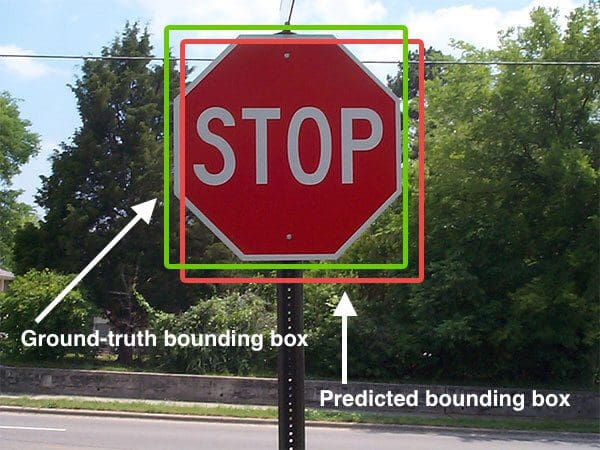
\includegraphics[scale=0.49]{pictures/iou_stop_sign.jpg}
            \caption{Die vorhergesagte Boundingboxe wird in Rot dargestellt, während die Ground-Truth-Boundingboxe in Grün dargestellt wird.\cite{iou}}
        \end{figure}

\newpage
        \cite{iou}
        Die IoU zwischen der vorhergesagten Boundingbox und der Ground-Truth-Boundingbox lässt sich einfach berechnen:
        Die Fläche der Schnittmenge wird durch die Fläche der Vereinigung der beiden Boundingboxen dividiert.
        
        \begin{center}  
            $Area = x2 y2 - x1 y1$\\
            wobei $x1y1$ obere linke Ecke und $x2y2$ untere rechte Ecke\\ \bigskip
            \large$IoU = \frac{Area_{Ground-Truth} \cap Area_{predicted}}{Area_{Ground-Truth} \cup Area_{predicted}}$
        \end{center}

        \begin{figure}[!htb]
            \centering
            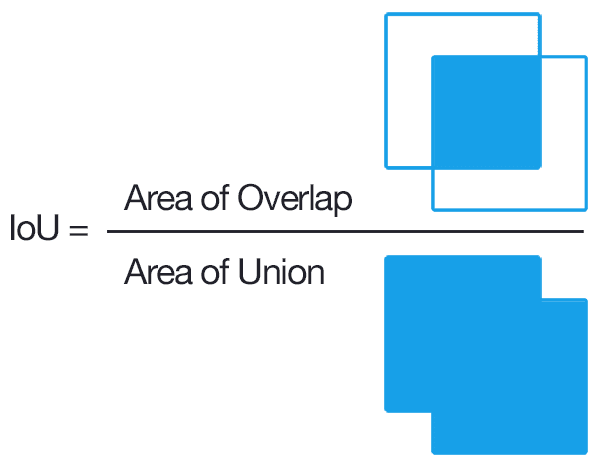
\includegraphics[scale=0.49]{pictures/iou_equation.png}
            \caption{Berechnung des IoU als Grafik.\cite{iou}}
        \end{figure}

        Bei der Verwendung von IoU als Bewertungsmetrik muss ein Schwellenwert (Threshold) für die Genauigkeit festgelegt werden, der in der Regel bei 0,5 liegt. Werte darüber werden als gut bewertet, während Werte darunter als unbrauchbar gelten.\cite{iou_paper, iou_2}

\chapter{Konzept}
    Wie in der Einleitung bereits erwähnt, stellt die begrenzte Bandbreite beim autonomen Fahren eine Herausforderung dar, da die enormen Datenmengen die verfügbaren Ressourcen schnell überlasten. Eine mögliche Lösung besteht darin, die Bilder zu verkleinern, bevor sie in die Cloud hochgeladen werden.
    
    Ziel dieser Arbeit ist es, Originalbilder, Bilder mit nicht KI-basierter Kompression im verlustbehafteten Format JPEG sowie Bilder, die mit KI-basierter Kompression reduziert und anschließend rekonstruiert wurden, miteinander zu vergleichen. Dabei sollen Rückschlüsse und Erkenntnisse über die Qualität der Bilder im Vergleich zu den Originalbildern sowie untereinander gewonnen werden. Zusätzlich sollen mögliche Zusammenhänge, Abhängigkeiten oder Kausalitäten identifiziert werden.
    Dies wird mithilfe der bereits vorgestellten Metriken durchgeführt, um die Bildqualität in Abhängigkeit von der Art und Intensität der Kompression zu bewerten.
    Zunächst muss für die Aufgabendomäne des autonomen Fahrens ein passender Datensatz ausgewählt werden. Schließlich sollen reale, domänenspezifische Daten verwendet werden. Geeignet hierfür sind Datensätze wie KITTI, CamVid und Cityscapes. In dieser Arbeit wurde der Datensatz Cityscapes gewählt, da er besonders hochauflösende Bilder aus realen Straßenszenen im Straßenverkehr enthält.

    \begin{figure}[!htb]
        \centering
        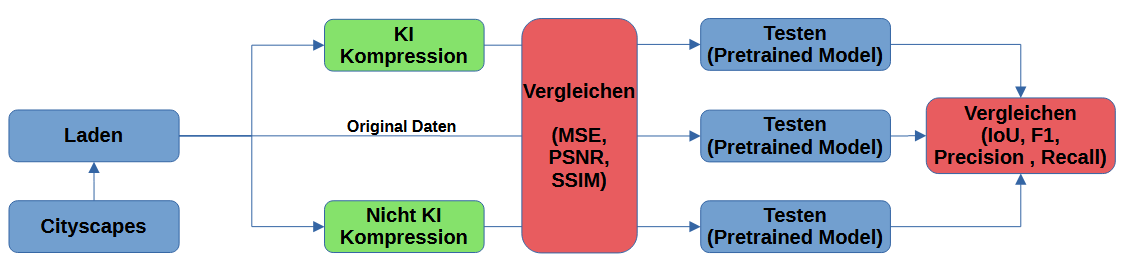
\includegraphics[scale=0.49]{pictures/PAP_2.0.png}
        \caption{PAP Diagramm welches das Vorgehen dieser Arbeit veranschaulicht.}
    \end{figure}
    
    Zunächst wird der Cityscapes-Datensatz zweimal dupliziert und aufgeteilt. Ein Datensatz wird in ein VQ-VAE-Modell eingespeist, wodurch die KI-komprimierten und rekonstruierten Daten erzeugt werden. Der andere Datensatz wird mit einem nicht-KI-basierten Verfahren komprimiert, wobei hier JPEG, ein verlustbehaftetes Bildformat, verwendet wird. So entstehen neben dem Originaldatensatz auch KI-rekonstruktierte Daten sowie JPEG-komprimierte Daten.
    
    Die JPEG-komprimierten Daten sowie die durch KI erzeugten Daten werden mit den Originaldaten abgeglichen und verglichen. Die Metriken, die in diesem Schritt verwendet werden, um Rückschlüsse zu ziehen, sind MSE, PSNR und SSIM.
    Diese Metriken geben Aufschluss über die Qualität der Bilder im Vergleich zu ihrem Original.
    Es gibt verschiedene Kompressionsstufen, die unterschiedliche Ergebnisse liefern, wenn sie auf ihre Qualität untersucht werden. So werden die KI-erzeugten und die JPEG-Daten ebenfalls hinsichtlich ihrer Qualität in Abhängigkeit von der Kompressionsstufe untersucht.
    Im nächsten Schritt werden die drei Datensätze in ein Modell eingegeben, das auf den Bildern Objekte detektiert und Boundingboxen um diese legt. Der Originaldatensatz dient dabei als Label und enthält die Ground-Truth-Boundingboxen.
    Es wird erneut verglichen, wie die KI-generierten Daten und die JPEG-Daten im Vergleich zu den Ground-Truth-Daten abschneiden. Hierfür werden Metriken wie Precision, Recall und F1-Score verwendet sowie der IoU (Intersection over Union), um zu untersuchen, wie gut Vorhersagen getroffen werden. 
    Ob in den Boundingboxen der Labels tatsächlich das richtige Objekt zu erkennen ist oder nicht, spielt keine Rolle. Sie dienen als Ground-Truth-Boundingboxen, anhand derer die rekonstruierten und komprimierten Bilder gemessen werden, die versuchen müssen, diese so gut wie möglich zu approximieren.
\chapter{Modelle} 
    \cite{rombach2021highresolution, https://doi.org/10.48550/arxiv.2204.11824} In dieser Arbeit werden zwei Modelle zur Bildreduktion und Rekonstruktion verwendet. Beide Modelle sind\\
    \textbf{Vector-Quantised-Variational-Autoencoder (VQ-VAE)},\\
    die mithilfe eines Codebooks die latente Darstellung abbilden und daraus das Bild rekonstruieren.\\
    Beide VQ-VAEs haben die Spezifikationen f, VQ(Z, d).\\
    \textbf{vq-f16}: f=16, VQ (Z=16384, d=8)\\
    \textbf{vq-f8-n256}: f=8, VQ (Z=256, d=4)
    
    \begin{itemize} \item \( f \): \textbf{Patch-Größe}
        \begin{itemize}
            \item \( f \) Steht für die Größe der Bildpatches in die das Eingabebild unterteilt wird.
                    Die Patch-Größe bestimmt die räumliche Auflösung der latenten Darstellung.
            \item Für \( f = 16 \) wird das Bild in \( 16 \times 16 \)-Pixel große Blöcke (Patches) zerlegt.\\
            Für \( f = 8 \) in \( 8 \times 8 \)-Pixel große Blöcke.
        \end{itemize}
    \end{itemize}

    \begin{itemize} \item \( Z \): \textbf{Codebuchgröße}
        \begin{itemize}
            \item \( Z \) ist die Größe des Codebuchs, also die Anzahl der Vektoren\\(Codebook-Vektoren),
            die für die Repräsentation der Patches verfügbar sind.
            Jeder Patch wird auf einen Vektor aus diesem Codebuch abgebildet.
            \item Ein größeres Codebuch (z.B. $Z=16384$) bietet eine feinere Auflösung der Quantisierung, während ein kleineres Codebuch (z.B. $Z=256$) weniger Speicherplatz benötigt, aber potenziell Informationen verliert.
        \end{itemize}
    \end{itemize}

    \begin{itemize} \item \( d \): \textbf{Latente Dimension}
        \begin{itemize}
            \item \( d \) ist die Dimension der latenten Repräsentation eines jeden Patches nach der Quantisierung. Ein Patch von Größe $f \times f$ wird auf einen latenten Vektor der Länge $d$ reduziert.
            \item Für $d=8$ wird ein Patch auf einen 8-dimensionalen Vektor komprimiert.\\
            Für $d=4$ ist die Kompression stärker, da die Information in nur 4 Dimensionen kodiert wird.
        \end{itemize}
    \end{itemize}

\newpage
    \section{Theoretische Kompression}
        \cite{rombach2021highresolution, https://doi.org/10.48550/arxiv.2204.11824} Beide Modelle nehmen die gleichen Bilder entgegen, liefern jedoch unterschiedlich große latente Repräsentationen. Ein Bild hat die Größe $(3 \times 1024 \times 2048)$ und liegt als float32 (4 Bytes) vor, welches vom Modell entgegengenommen wird.
        
        \begin{enumerate}
        \item \textbf{Latente Darstellung vq-f16}: f=16, VQ (Z=16384, d=8)\\
            \textbf{f = 16:} Das Bild wird in Blöcke von $16 \times 16$ Pixeln zerlegt.
            \begin{addmargin}[45pt]{0pt}
            Anzahl der Blöcke in der Höhe: $1024 \div 16 = 64$\\
            Anzahl der Blöcke in der Breite: $2048 \div 16 = 128$
            \end{addmargin}
            \textbf{d = 8:} Jeder Block wird auf einen Vektor der Dimension 8 abgebildet.\\
            Latent Shape: ($8 \times 64 \times 128$)
        \item \textbf{Latente Darstellung vq-f8-n256}: f=8, VQ (Z=256, d=4)\\
            \textbf{f = 8:} Das Bild wird in Blöcke von $8 \times 8$ Pixeln zerlegt.
            \begin{addmargin}[45pt]{0pt}
            Anzahl der Blöcke in der Höhe: $1024 \div 8 = 128$\\
            Anzahl der Blöcke in der Breite: $2048 \div 8 = 256$
            \end{addmargin}
            \textbf{d = 4:} Jeder Block wird auf einen Vektor der Dimension 4 abgebildet.\\
            Latent Shape: ($4 \times 128 \times 256$)
        \end{enumerate}
    
        Da es sich um VQ-VAEs handelt, werden die Einträge der latenten Vektoren auf die Einträge des Codebuchs abgebildet. Die Einträge des Codebuchs sind fest, d.h. es reicht aus, lediglich die Indizes der Codebuch-Einträge zu speichern. Es wird also keine kompletten 4 Bytes (float32) benötigt, sondern lediglich die Anzahl an Bits, um die Codebuchgröße $Z$ darzustellen.
        
        \begin{center}  
                $\text{Anzahl Werte} = 3 * 1024  * 2048 = 6.291.456$ \\
                $\text{Speicherbedarf (Bytes)} = 6.211.548 * 4 \text{Byte} = 25.165.824 \text{Bytes}$\\
                $Z_{vq-f16} = 16384 \quad 14\text{Bits} = \frac{\ln{16384}}{\ln{2}}$\\
                $25.165.824\text{Bytes} \div (8 * 64 * 128 * \frac{14}{8}\text{Bytes}) \approx 219,43$
                $Z_{vq-f8-n256} = 256 \quad 8\text{Bits} = \frac{\ln{256}}{\ln{2}}$\\
                $25.165.824\text{Bytes} \div (4 * 128 * 256 * \frac{8}{8}\text{Bytes}) = 192$
         \end{center}

        Somit ergibt sich ein Kompressionsfaktor von $219,43$ für vq-f16 und $192$ für vq-f8-n256.
\chapter{Evaluation}
    \section{Beschreibung der verwendeten Daten}
        Als Datenbasis wurde Cityscapes verwendet. Es ist ein bekannter Datensatz im Bereich der Bildsegmentierung und der Computer Vision. Der Datensatz wurde speziell für Aufgaben entwickelt, die sich auf urbane Regionen beziehen. Autonomes Fahren ist eine der Domänen, für die sich der Cityscapes-Datensatz ideal eignet. Die Motivation hinter diesem Datensatz ist es, realistische urbane Szenen aus echten Verkehrssituationen abzubilden. Der Cityscapes-Datensatz soll die Lücke schließen, da bisherige Datensätze die Komplexität realer urbaner Szenen nicht ausreichend widerspiegeln.
        In der Forschung dient der Datensatz auch als Benchmark für verschiedene Algorithmen \cite{cityscapes_paper, cityscapes, cityscapes2}.

        \begin{figure}[!htb]
            \centering
            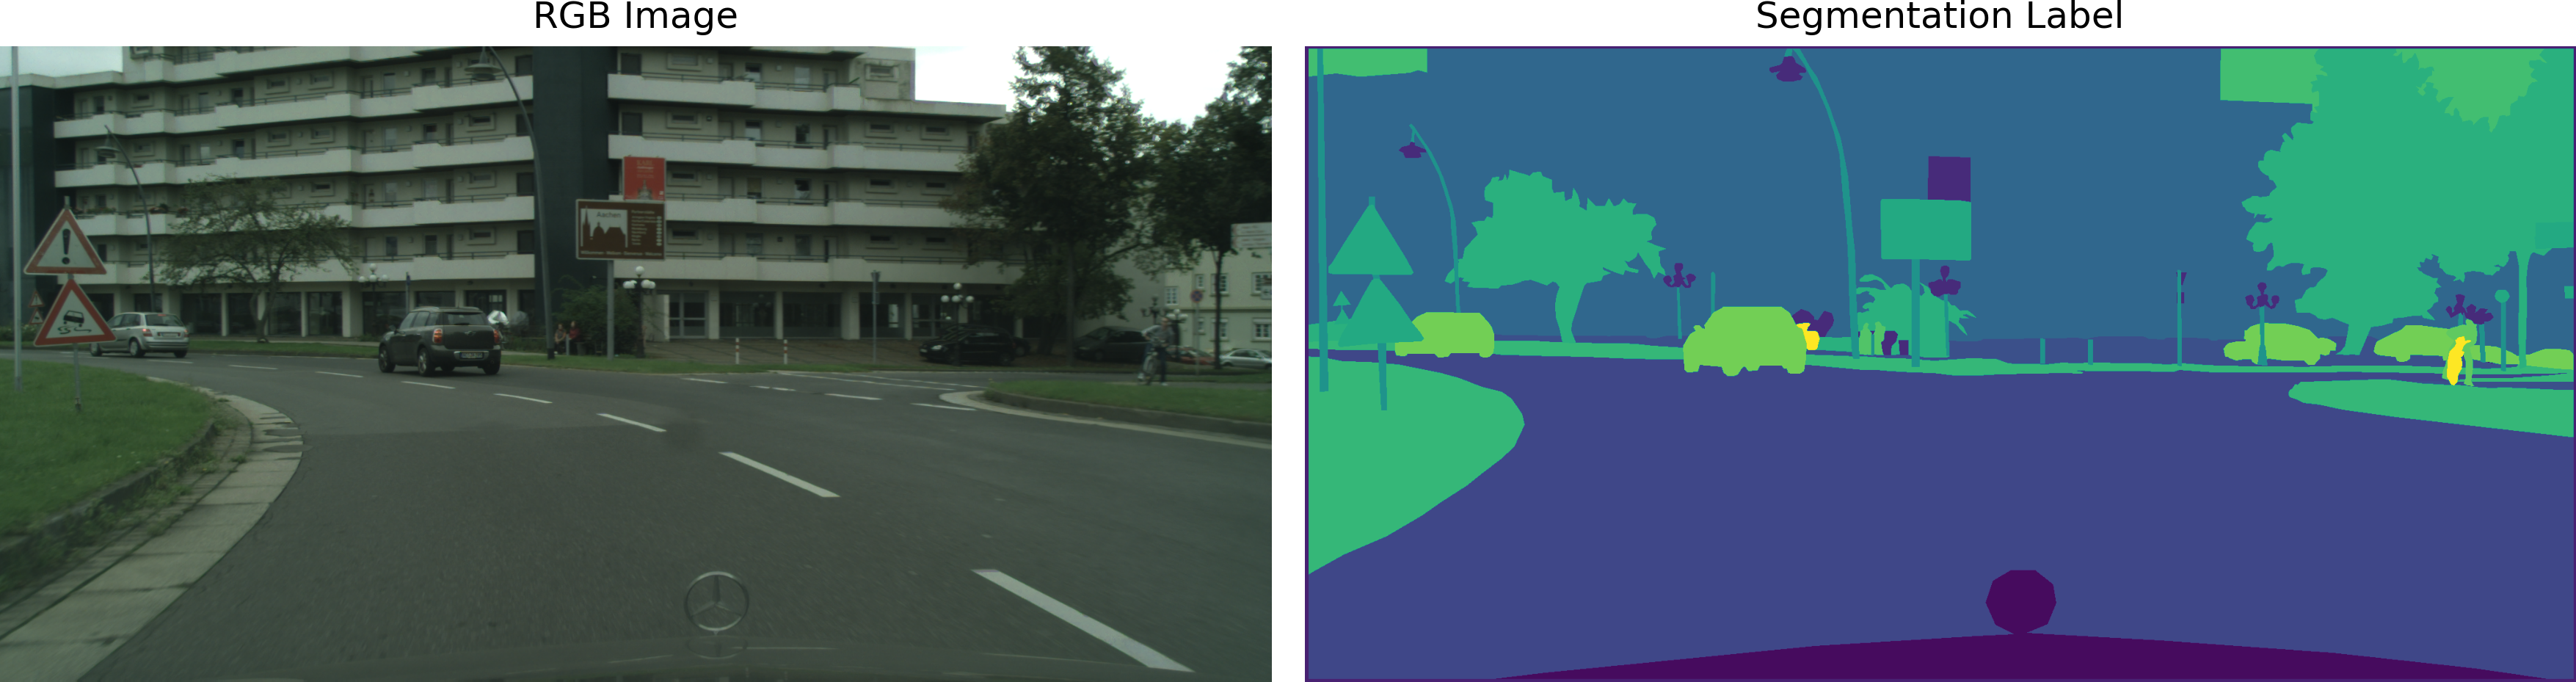
\includegraphics[scale=0.49]{pictures/output_plot_0.png}
            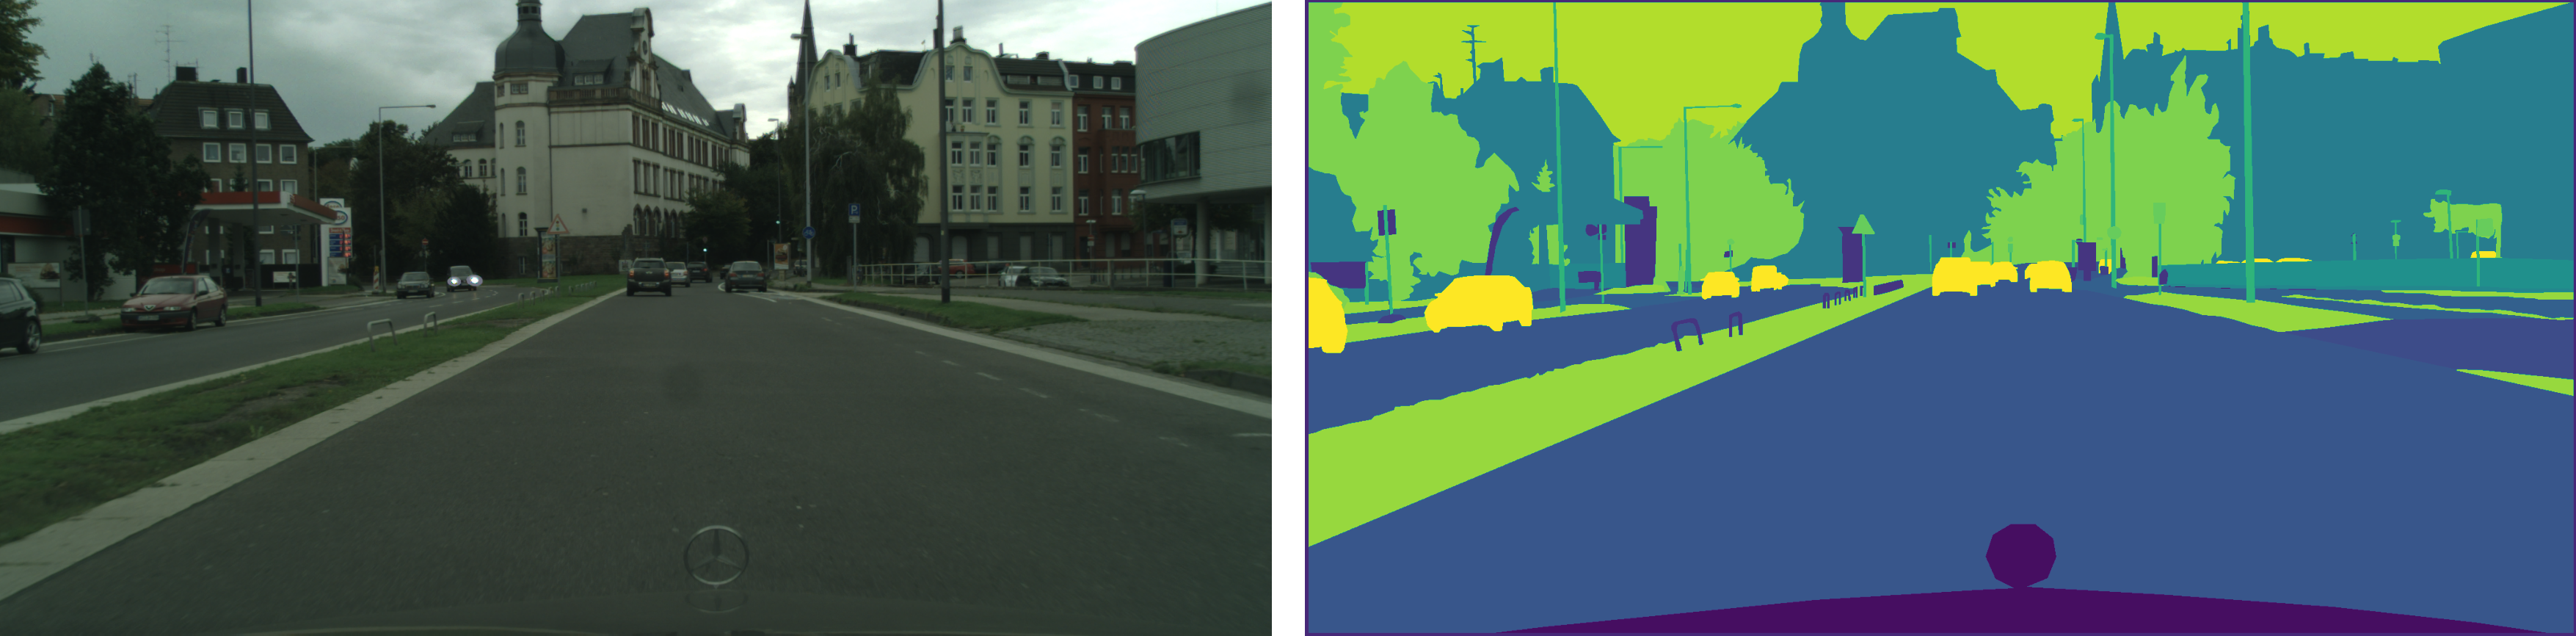
\includegraphics[scale=0.49]{pictures/output_plot_1.png}
           \caption{Die ersten zwei Bilder des Cityscapes-Datensatz aus Aachen.}
        \end{figure}

\newpage
        \subsection{Aufbau des Datensatzes}
            Der Datensatz besteht aus Bildern urbaner Szenen, aufgenommen aus $50$ verschiedenen europäischen Städten.
            Die Daten wurden mit Dashcams erfasst, die an Fahrzeugen angebracht waren. Die Bilder sind in RGB mit einer Auflösung von 2k $(2048 \times 1024)$ und haben den sogenannten Shape $(3, 2048, 1024)$. Sie liegen als verlustfreie PNG-Dateien vor.
            Diese sind in drei Kategorien unterteilt, jeweils mit entsprechenden Labels. Insgesamt umfasst der Datensatz $5000$ hochqualitative Pixel-Level-Annotationen, davon $2975$ für das Training, $500$ für die Validierung und $1525$ für den Test. Zudem enthält der Datensatz $20.000$ grob annotierte Bilder.\newline
      
            Die Labels sind in $8$ Kategorien unterteilt, mit insgesamt $30$ Klassen. Der Fokus liegt auf dem Straßenverkehr, einschließlich Autos, Fußgängern, Gebäuden und der Infrastruktur \cite{cityscapes_overview, cityscapes_paper}. 
            \begin{enumerate}
            \item \textbf{Fläche (Flat):}
                \begin{itemize}
                    \item Straße (road)
                    \item Gehweg (sidewalk)
                    \item Parkplatz (parking)
                    \item Schienenstrang (rail track)
                \end{itemize}
                \item \textbf{Menschen (human):}
                    \begin{itemize}
                    \item Fußgänger (person)
                    \item Fahrradfahrer (rider)
                \end{itemize}
                \item \textbf{Fahrzeuge (Vehicle):}
                \begin{itemize}
                    \item Auto (car)
                    \item Motorrad (motorcycle)
                    \item Fahrrad (bicycle)
                    \item Bus (bus)
                    \item LKW (truck)
                    \item Wohnmobil (caravan)
                    \item Schienenfahrzeuge (on rails)
                    \item Anhänger (trailer)
                \end{itemize}

\newpage
                \item \textbf{Konstruktionen (Construction):}
                \begin{itemize}
                    \item Gebäude (building)
                    \item Mauer (wall)
                    \item Zaun (fence)
                    \item Brücke (bridge)
                    \item Tunnel (tunnel)
                    \item Schutzgeländer (guard rail)
                \end{itemize}
                \item \textbf{Objekte (object):}
                \begin{itemize}
                    \item Polster (pole)
                    \item Ampelmasten (polegroup)
                    \item Ampel (traffic light)
                    \item Verkehrsschild (traffic sign)
                \end{itemize}
                \item \textbf{Natur (nature):}
                \begin{itemize}
                    \item Vegetation (vegetation)
                    \item Terrain (terrain)
                \end{itemize}
                \item \textbf{Himmel (sky):}
                \begin{itemize}
                    \item Himmel (sky)
                \end{itemize}
                \item \textbf{Leer (void):}
                \begin{itemize}
                    \item Alle anderen Strukturen (ground)
                    \item Temporäre Dinge (dynamic)
                    \item Hintergrund, andere Objekte (static)
                \end{itemize}
            \end{enumerate}

            Die vorhandenen Labels werden jedoch \textbf{nicht} verwendet, da für diese Arbeit eigene Labels mithilfe eines vortrainierten Modells erzeugt werden, um als Ground-Truth-Daten zu dienen.

\newpage 
    \section{Vergleich der Bilder}
        \subsection{JPEG-komprimierte Bilder}
            Die Problemdomäne dieser Arbeit ist die Reduzierung von Bilddaten, um diese im Kontext des autonomen Fahrens effizient in die Cloud hochladen und dort rekonstruieren zu können.

            Bei traditionellen Kompressionsverfahren entfällt der Teil der Rekonstruktion. Hierbei wird das Bild lediglich räumlich reduziert. Eines der bekanntesten verlustbehafteten Kompressionsverfahren ist das JPEG-Format. 
        
            Zunächst werden die Originalbilder in JPEG-Datensätze mit verschiedenen\\
            Kompressionsstufen dupliziert. Ziel ist es, die unterschiedlichen JPEG-Datensätze sowohl untereinander als auch im Vergleich zu den Originaldaten zu untersuchen. Hierfür werden die drei Metriken SSIM, PSNR und MSE angewendet. Da JPEG ein verlustbehaftetes Kompressionsverfahren ist, erfolgt die räumliche Reduzierung der Bilder auf Kosten ihrer Qualität.
            Der Faktor der Kompressionsqualität kann vom Anwender festgelegt werden und wird prozentual angegeben.
            Eine Kompressionsqualität von $100\%$ entspricht nahezu dem Original, ist jedoch ebenfalls verlustbehaftet, wie in Abbildung \ref{fig:og_hundred} zu sehen ist.
            Eine niedrigere Kompressionsqualität, beispielsweise $20\%$, führt zu deutlich sichtbaren Qualitätsverlusten, spart jedoch erheblich mehr Speicherplatz. Je geringer die Kompressionsqualität, desto ausgeprägter sind die Artefakte, die bei stark komprimierten Bildern auftreten.
               
            In dieser Arbeit wurden mittels JPEG-Kompression 15 neue Datensätze unterschiedlicher Kompressionsqualitäten (in \%) erzeugt. Diese basieren auf dem original im PNG-Format vorliegenden Datensatz, der aus den 2975 hochauflösenden
            2K-RGB-Bildern besteht.\newline
            \[
            \begin{array}{|p{0.5cm}|p{0.5cm}|p{0.5cm}|p{0.5cm}|p{0.5cm}|p{0.5cm}|p{0.5cm}|p{0.5cm}|p{0.5cm}|p{0.5cm}|p{0.5cm}|p{0.5cm}|p{0.5cm}|p{0.5cm}|p{0.5cm}|} \hline \scriptsize 5 & \scriptsize 10 & \scriptsize 15 & \scriptsize 20 & \scriptsize 25 & \scriptsize 30 & \scriptsize 40 & \scriptsize 50 & \scriptsize 60 & \scriptsize 70 & \scriptsize 75 & \scriptsize 85 & \scriptsize 90 & \scriptsize 95 & \scriptsize 100 \\ \hline \end{array}
            \]
            Dabei zeigte sich, dass die prozentuale Dateigröße im Vergleich zum Original \textbf{nicht linear} von der Kompressionsqualität abhängt.

\newpage 
            \underline{\textbf{Kompression in Bezug auf den Speicherbedarf}}        
            \begin{figure}[!htb]
                \centering
                \includesvg[scale=0.56]{graphs/output_plot_size_images.svg}
                \caption{Diese Grafik zeigt den Speicherplatz Bedarf der einzelnen Datensätze entsprechender Kompressionsqualitäten in $\%$, im Vergleich zum Originaldatensatz.}
                \label{fig:speicher_kompressionsqualität}
            \end{figure}

            Je geringer die Kompressionsqualität, desto kleiner wird die Bildgröße, was Speicherplatz spart. Dabei zeigt sich, dass der größte Unterschied der Speichergröße sich im Bereich von $95\%$ und $100\%$ Kompressionsqualität abspielt mit einer Differenz von bis zu $29,5\%$. Zwischen $85\%$ und $100\%$ sind es $39,6\%$. Mit abnehmender Kompressionsqualität sinken die Dateigrößen also drastisch ab, bis zu $85\%$ Kompressionsqualität ist dies am deutlichsten zu sehen. Unterhalb flacht die Kurve ab. Unter $70\%$ macht die Kompressionsqualität kaum noch einen Unterschied hinsichtlich des Speicherbedarfs.
            Von $5\%$ bis zu $70\%$ Kompressionsqualität gibt es über $65$ Einheiten hinweg lediglich einen Unterschied in der Dateigröße von gerade einmal $4,8\%$ Differenz. Wenn man dies im Vergleich mit der Differenz zwischen $85\%$ bis $100\%$, welche sich über $15$ Einheiten erstreckt, so ist diese um ein achtfaches kleiner auf mehr als viermal so vielen Einheiten hinweg. Die Standardabweichung (helle Schattierung) zeigt, dass die Varianz in der Dateigröße bei niedriger Kompressionsqualität sehr gering ist, aber mit steigender Qualität zunimmt. Dies könnte auf unterschiedliche Bildinhalte und die ineffiziente Speicherung bei hohen Qualitätsstufen hinweisen.

\newpage
            Die obige Grafik (Abbildung \ref{fig:speicher_kompressionsqualität}) zeigt jedoch nur das Verhältnis zwischen der Kompressionsqualität und der prozentualen Größe des Bildes auf dem Datenträger im Vergleich zum Originaldatensatz. Sie gibt jedoch noch keine Auskunft über den genauen Kompressionsfaktor. Dieser spielt eine wichtige Rolle, da er möglichst groß sein sollte, ohne die Qualität des Bildes zu sehr zu beeinträchtigen.
            
            \begin{figure}[!htb]
                \centering
                \includesvg[scale=0.56]{graphs/output_plot_ratio_images.svg}
                \caption{Diese Grafik zeigt den Kompressionsfaktor der einzelnen Datensätze entsprechend ihrer
                Kompressionsqualitäten in $\%$}
                \label{fig:speicher_kompressionsfaktor}
            \end{figure}

            Man erkennt, dass der Kompressionsfaktor mit steigender Kompressionsqualität sinkt. Höhere Qualitätsstufen weisen weniger Kompression auf und somit werden größere Dateien erzeugt. Die Funktion besitzt einen Wendepunkt bei etwa $50\%$ 
            Kompressionsqualität. Zu Beginn, in den höheren Bereichen der Kompressionsqualität, von $75\%$ bis $100\%$ ist der Kompressionsfaktor gering, jedoch stärker abfallend um eine Differenz von $11,66$. Im Vergleich zu $50\%$ bis $75\%$ beträgt die Differenz nur $6,88$. Das Gleiche lässt sich bei Kompressionsqualitäten unterhalb des Wendepunkts beobachten. Während bei Werten von $25\%$ bis $50\%$ die Differenz kleiner ist als zwischen $5\%$ und $25\%$. Die Bereiche zwischen $60\%$ und $75\%$ können als der „Sweetspot“ angesehen werden, um einen guten Kompressionsfaktor und reduzierten Speicherbedarf zu erreichen bei Kompressionsqualitäten oberhalb des Wendepunkts.
            Die Grafik weist Ähnlichkeiten mit der der Funktion aus Abbildung \ref{fig:speicher_kompressionsqualität} auf, bei der ebenfalls ein minimaler Wendepunkt bei $50\%$ erkennbar ist.
            
\newpage  
            \underline{\textbf{Qualität der Bilder}}\bigskip

            \textbf{Kompressionsqualität (40)}
            \begin{figure}[!htb]
                \centering
                \begin{minipage}[!htb]{0.47\textwidth}
                    \centering
                    \textbf{Komprimiert} % Überschrift für die erste Spalte
                \end{minipage}
                %
                \begin{minipage}[!htb]{0.47\textwidth}
                    \centering
                    \textbf{Original} % Überschrift für die zweite Spalte
                \end{minipage}

                \begin{minipage}[!htb]{0.47\textwidth}
                    \centering
                    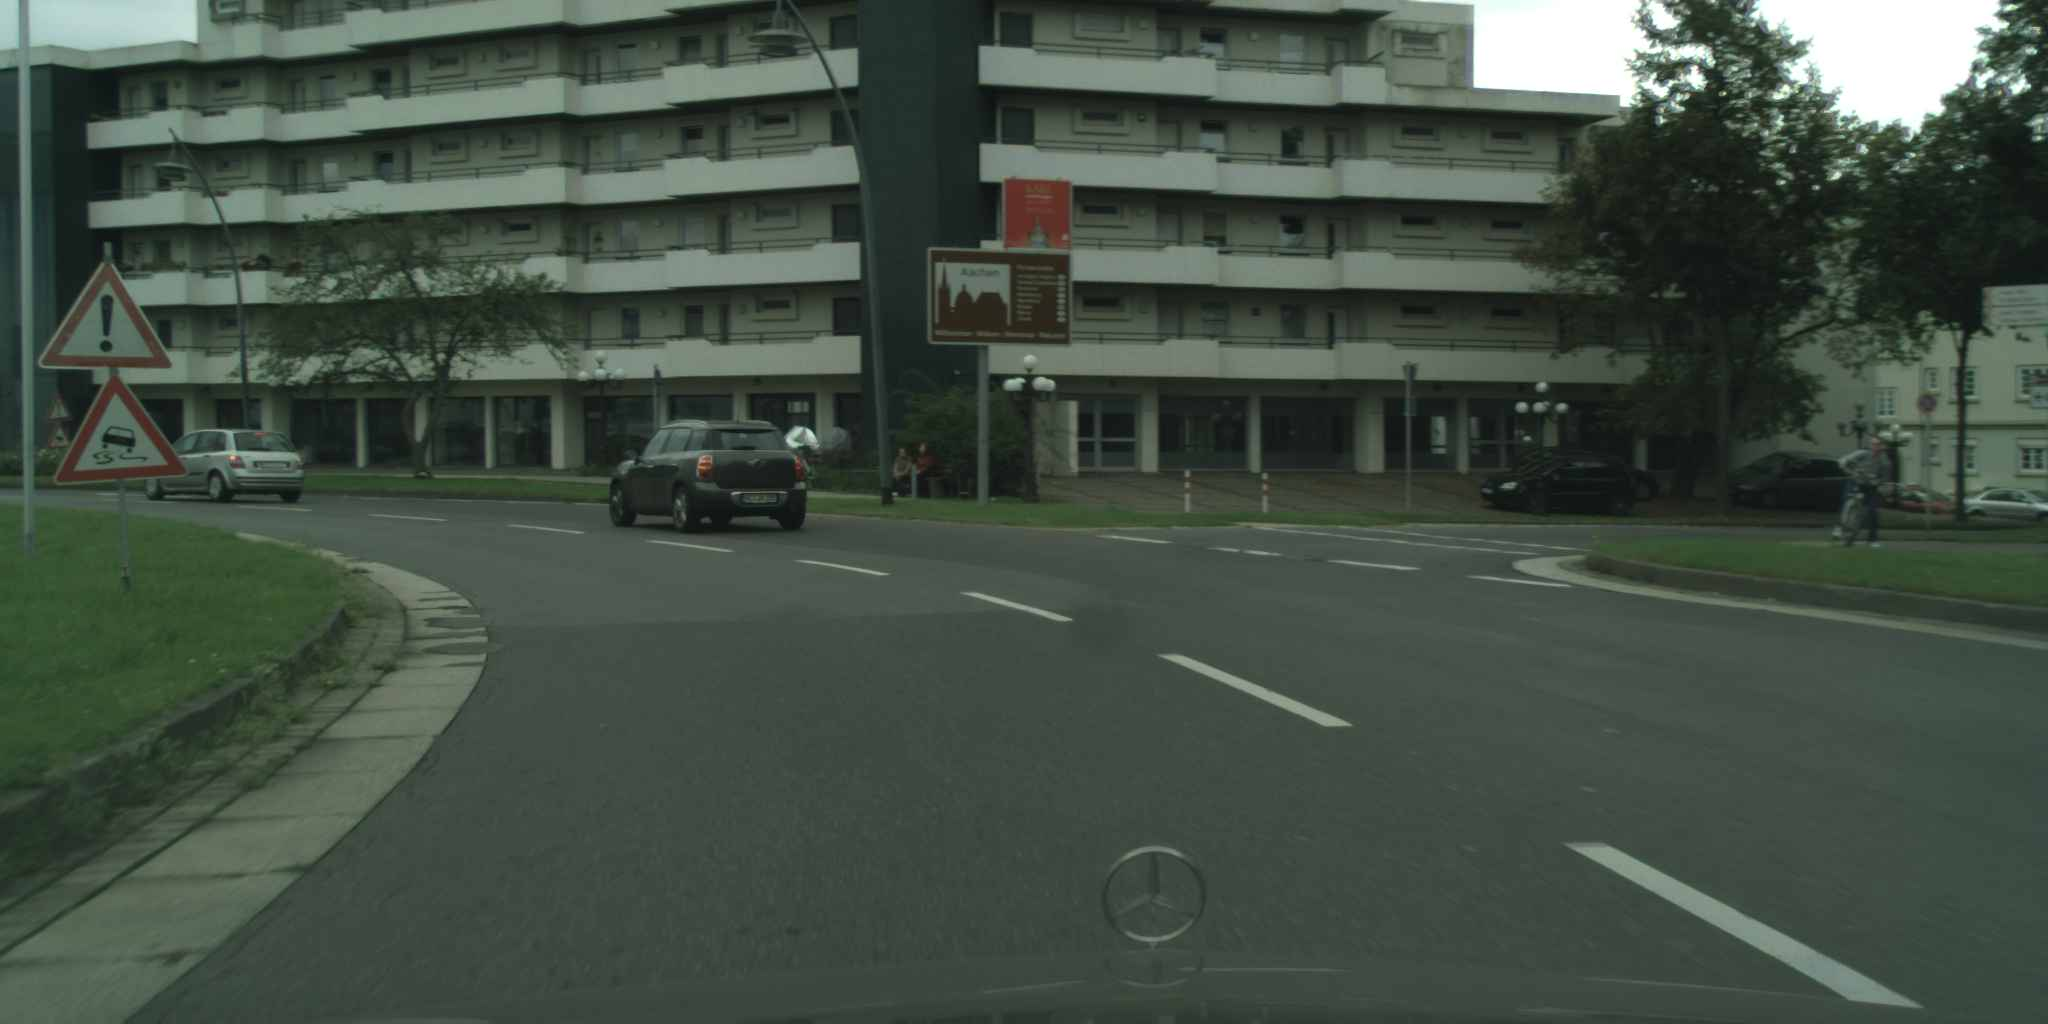
\includegraphics[width=\textwidth]{pictures/img00_jpg_40.jpg}    
                    \label{fig:bild5}
                \end{minipage}
                %
                \begin{minipage}[!htb]{0.47\textwidth}
                    \centering
                    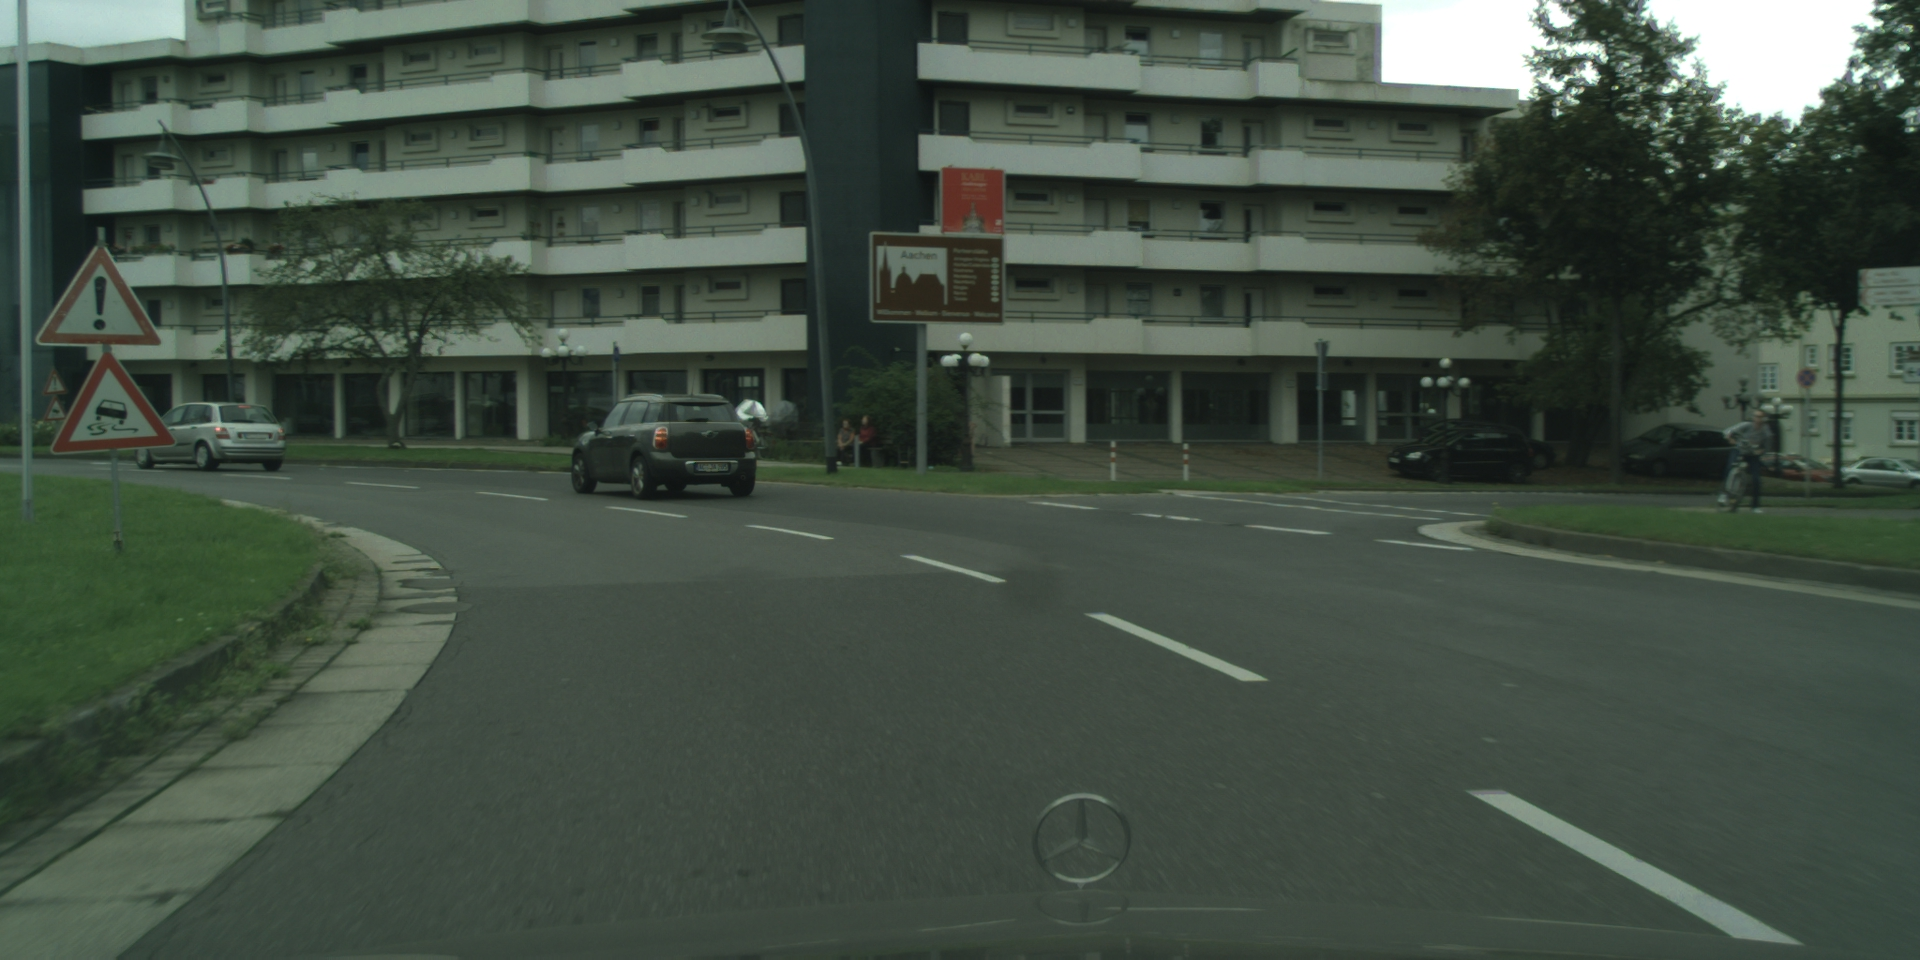
\includegraphics[width=\textwidth]{pictures/img00_png.jpg}
                    \label{fig:bild6}
                \end{minipage}
            \end{figure}
        
            \textbf{Kompressionsqualität (15)}
            \begin{figure}[!htb]
                \centering
                \begin{minipage}[!htb]{0.47\textwidth}
                    \centering
                    \textbf{Komprimiert} % Überschrift für die erste Spalte
                \end{minipage}
                %
                \begin{minipage}[!htb]{0.47\textwidth}
                    \centering
                    \textbf{Original} % Überschrift für die zweite Spalte
                \end{minipage}

                \begin{minipage}[!htb]{0.47\textwidth}
                    \centering
                    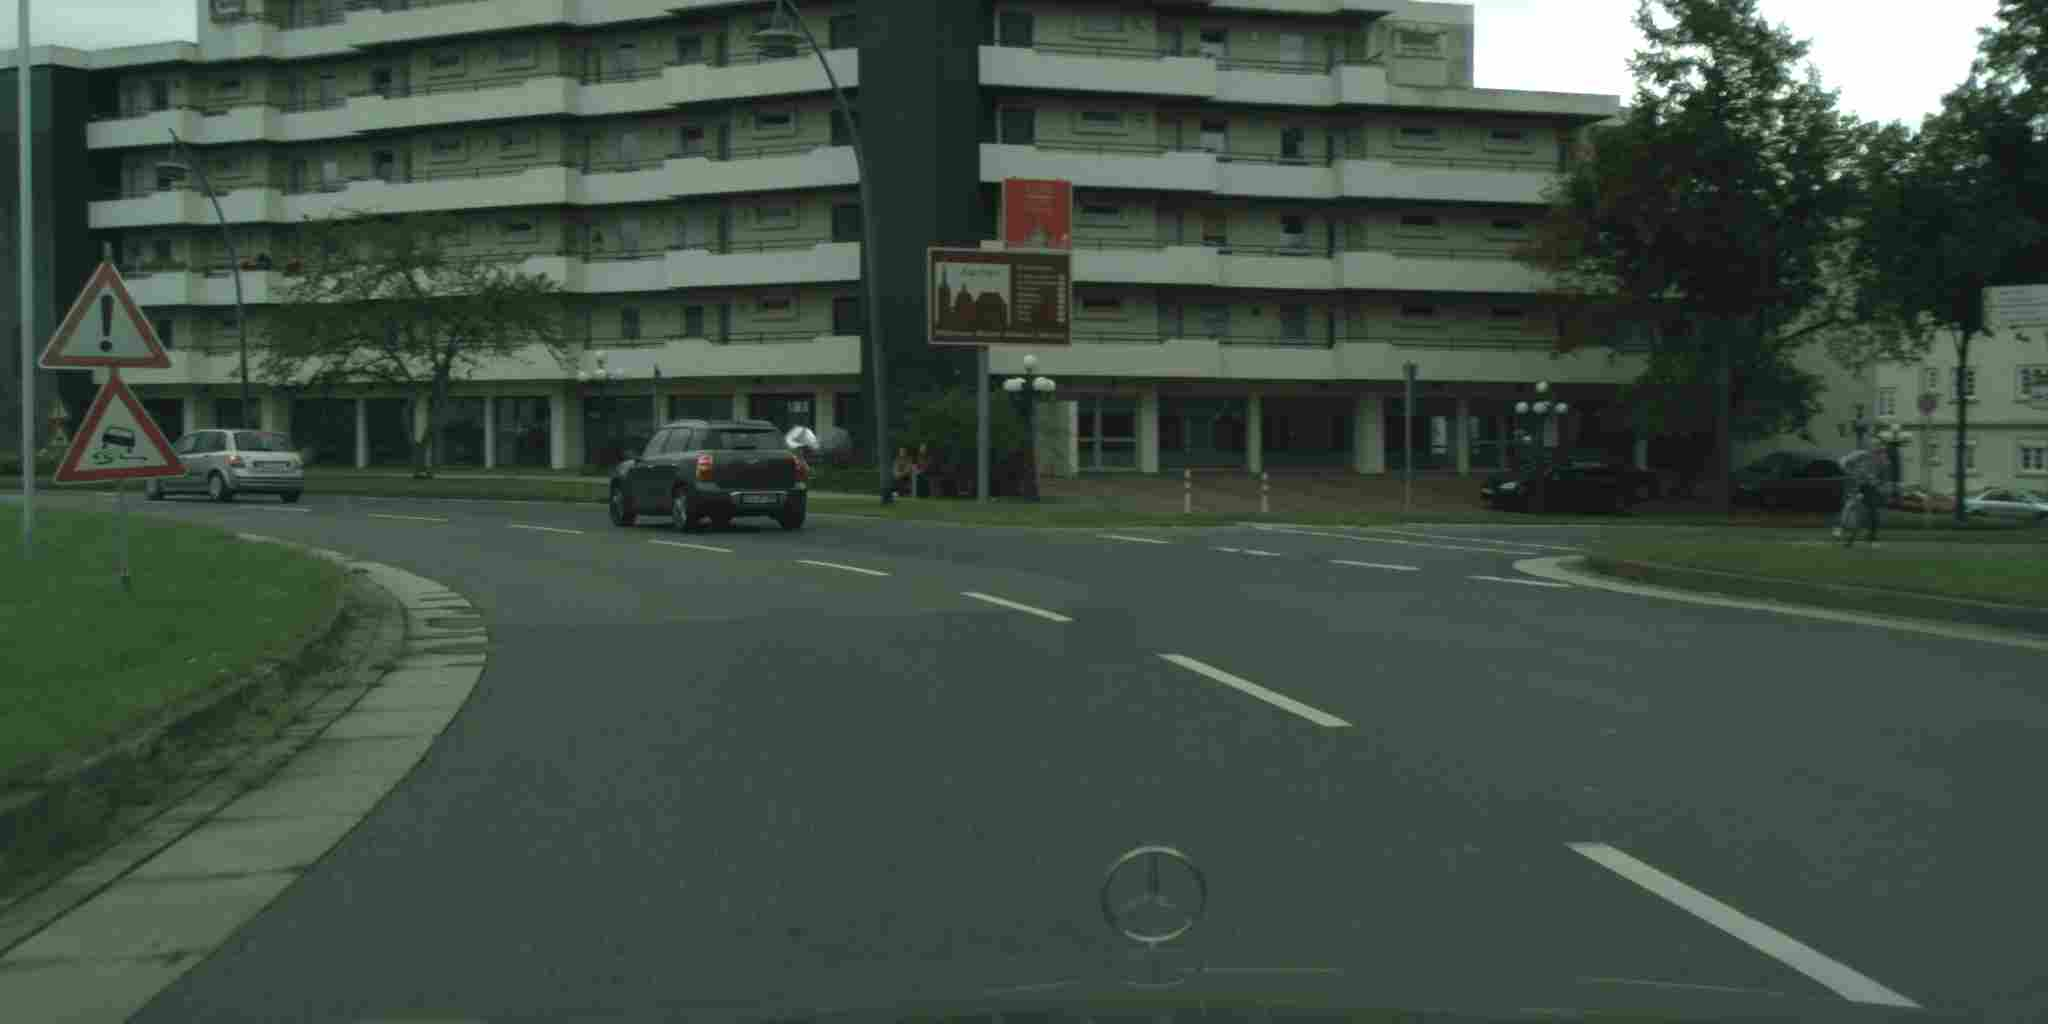
\includegraphics[width=\textwidth]{pictures/img00_jpg_15.jpg}    
                    \label{fig:bild9}
                \end{minipage}
                %
                \begin{minipage}[!htb]{0.47\textwidth}
                    \centering
                    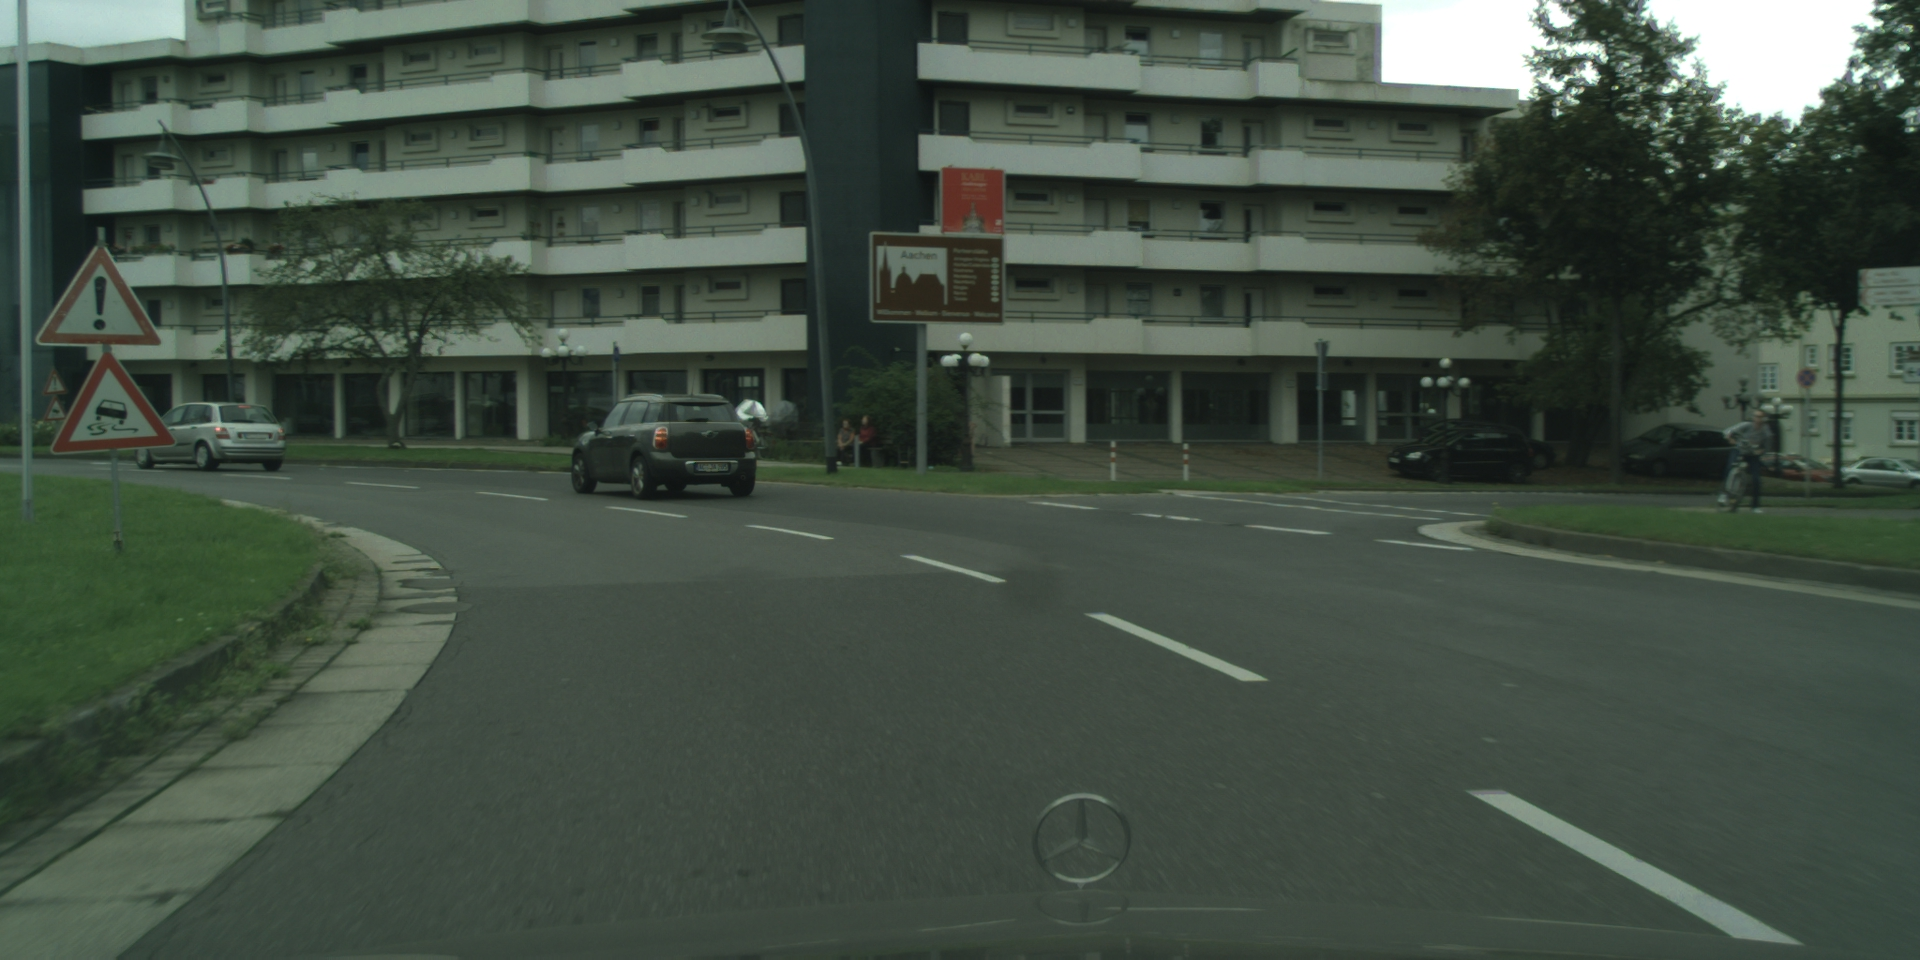
\includegraphics[width=\textwidth]{pictures/img00_png.jpg}
                    \label{fig:bild10}
                \end{minipage}
            \end{figure}

            \textbf{Kompressionsqualität (5)}
            \begin{figure}[!htb]
                \centering
                \begin{minipage}[!htb]{0.47\textwidth}
                    \centering
                    \textbf{Komprimiert} % Überschrift für die erste Spalte
                \end{minipage}
                %
                \begin{minipage}[!htb]{0.47\textwidth}
                    \centering
                    \textbf{Original} % Überschrift für die zweite Spalte
                \end{minipage}

                \begin{minipage}[!htb]{0.47\textwidth}
                    \centering
                    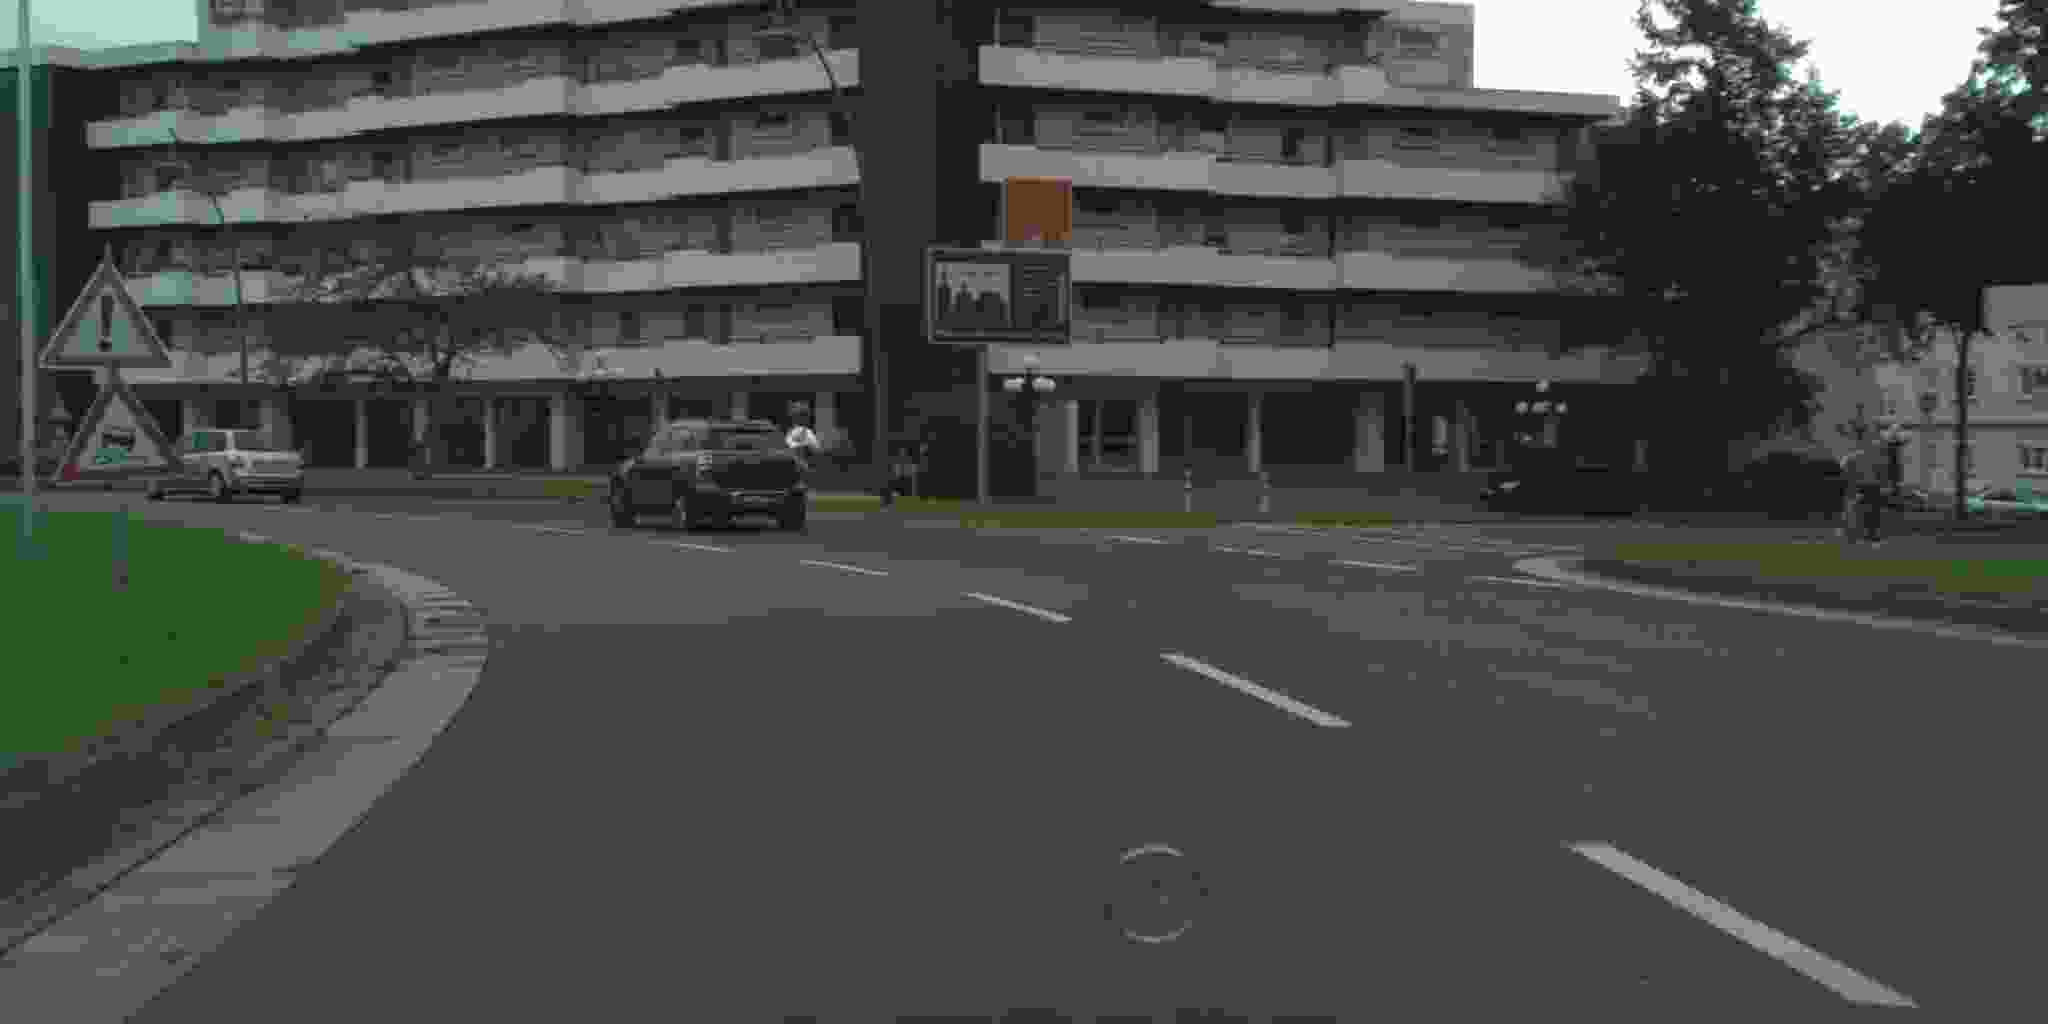
\includegraphics[width=\textwidth]{pictures/img00_jpg_5.jpg}    
                    \label{fig:bild13}
                \end{minipage}
                %
                \begin{minipage}[!htb]{0.47\textwidth}
                    \centering
                    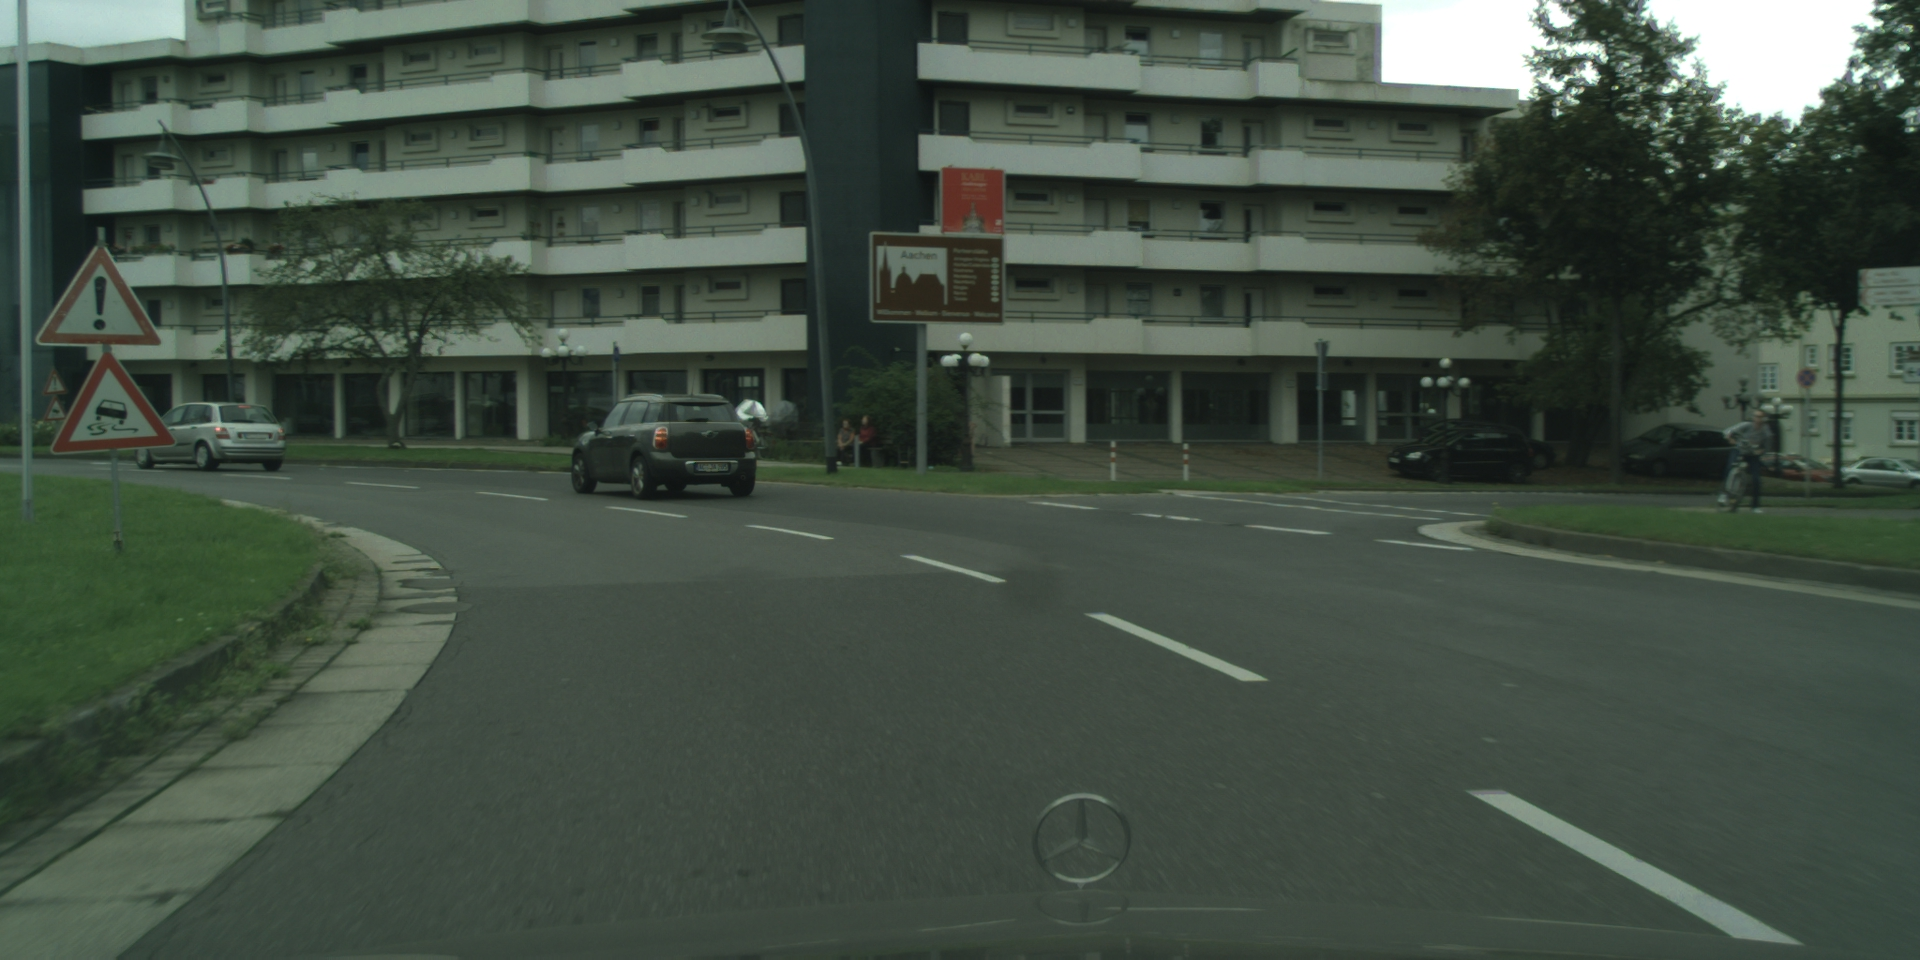
\includegraphics[width=\textwidth]{pictures/img00_png.jpg}
                    \label{fig:bild14}
                \end{minipage}
            \end{figure}

\newpage
            Interessant ist, dass sich JPEG-komprimierte Bilder anfangs kaum bis gar nicht voneinander unterscheiden, wenn man sie mit dem Original vergleicht. Erst bei einer Kompressionsqualität von etwa $15\%$ werden die Qualitätseinbußen des Bildes deutlich sichtbar. Auch bei einer Kompressionsqualität von $100\%$ ist die Bildqualität minimal schlechter als die des Originals. Dieser Unterschied ist jedoch mit dem menschlichen Auge nicht erkennbar, wie der folgende Bildvergleich zeigt.

            \begin{figure}[!htb]
                \centering
                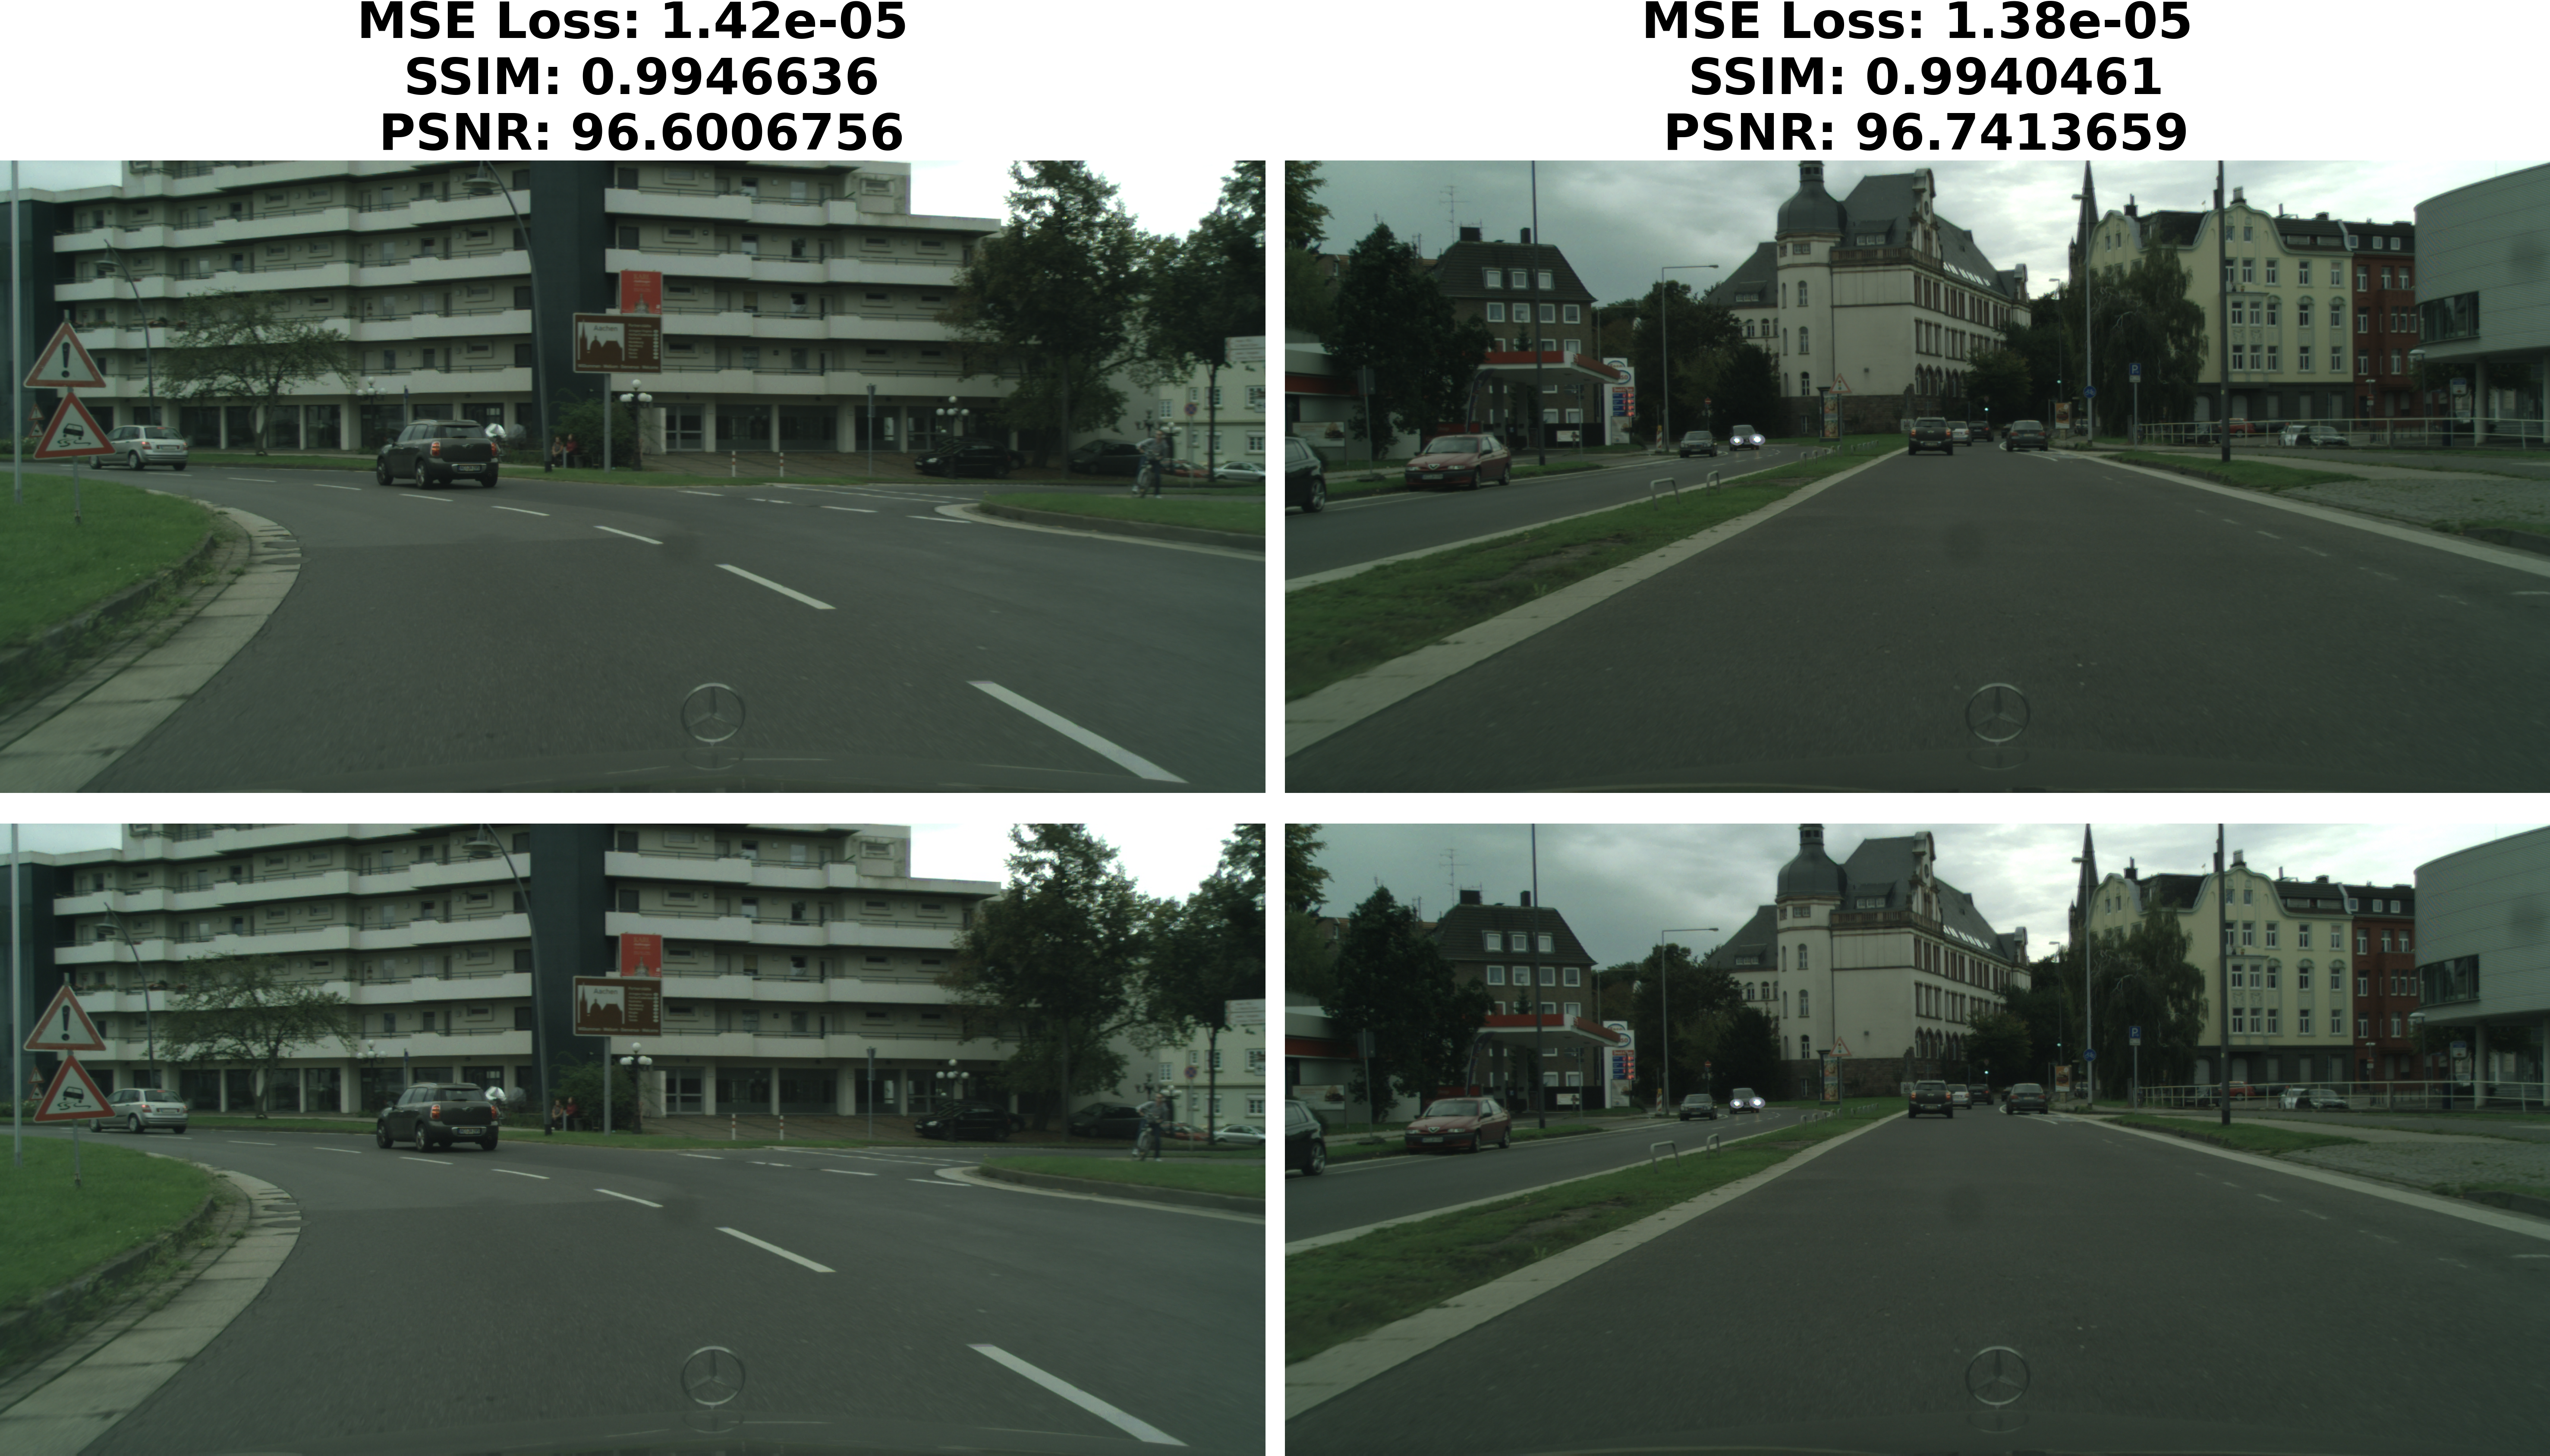
\includegraphics[scale=0.27]{pictures/output_plot_100.png}
                \caption{Oben das Original und unten das mit Kompressionsqualität von $100\%$ komprimierte JPEG-Bild.}
                \label{fig:og_hundred}
            \end{figure}

            Bei einem identischen Bild ohne Verluste würde der MSE $0.0$, der SSIM $1.0$ und der PSNR-Score $100$ betragen. Somit ist auch eine Kompressionsqualität von $100\%$ verlustbehaftet. Obwohl die Verluste verschwindend gering und mit dem menschlichen Auge nicht erkennbar sind, können sie mithilfe dieser Metriken nachgewiesen werden.\bigskip

            Die folgenden Grafiken zeigen den Qualitätsverlust, gemessen anhand von MSE, SSIM und PSNR, in Bezug auf die Kompressionsqualität in Prozent.

\newpage       
            \begin{figure}[!htb]
                \centering
                \includesvg[scale=0.56]{graphs/output_plot_mse.svg}
                \caption{Durchschnittswert MSE aller Bilder der JPEG-Datensätze.}
            \end{figure}

            \begin{figure}[!htb]
                \centering
                \includesvg[scale=0.56]{graphs/output_plot_ssim.svg}
                \caption{Durchschnittswert SSIM aller Bilder der JPEG-Datensätze.}
            \end{figure}
        
\newpage
            Die obere Grafik zeigt den MSE, die untere den SSIM. Es fällt direkt auf, dass der SSIM die Inverse zum MSE darstellt. Während der MSE mit $25\%$ einen Wert von $0,0003$ hat, steigt er unterhalb dieser Kompressionsqualität stark an auf ein sechseinhalb-faches bei $5\%$. Der SSIM hingegen, welcher sich stets von $100\%$ bis $25\%$ Kompressionsqualität in einem Wertebereich von $0,058$ bewegt hat, fällt unterhalb des Schwellenwerts von $25\%$ um ganze $0,3$ ab. Somit sollte man keine Kompressionsqualität unterhalb von $25\%$ wählen. Wie bereits in Abbildung \ref{fig:speicher_kompressionsqualität} zu sehen war, macht es für den Speicherbedarf unterhalb von $60-70\%$ keinen nennenswerten Unterschied mehr.
            
            \begin{figure}[!htb]
                \centering
                \includesvg[scale=0.56]{graphs/output_plot_psnr.svg}
                \caption{Durchschnittswert PSNR alle Bilder der JPEG-Datensätze.}
            \end{figure}

            Beim PSNR verhält es sich ähnlich wie in Abbildung \ref{fig:speicher_kompressionsfaktor}. Ein klarer Wendepunkt ist bei einer Kompressionsqualität von $50\%$ erkennbar. Oberhalb dieses Punktes fällt die Qualität von $100\%$ abwärts und flacht
            bis $50\%$ ab. Unterhalb dieses Wendepunkts fällt die Kurve bei abnehmender Kompressionsqualitäten immer stärker.      
        
            Bei Betrachtung der Grafiken und der Bilder unterschiedlicher Kompressionsqualitäten wird deutlich, warum die Bilder mit $100\%$ und $40\%$ Kompressionsqualität im Vergleich zum Original kaum voneinander zu unterscheiden waren. Die Grafiken zeigen, dass die Bildqualität erst ab einer Kompressionsqualität von $25\%$ bis $30\%$ sichtbar nachlässt.

            Eine Kompressionsqualität von ca. $80\%$ bietet einen guten Kompromiss, akzeptable Bildqualität (hohe PSNR- und SSIM-Werte) bei geringem Speicherbedarf.
            
        %\begin{figure}[!htb]
        %    \centering
        %    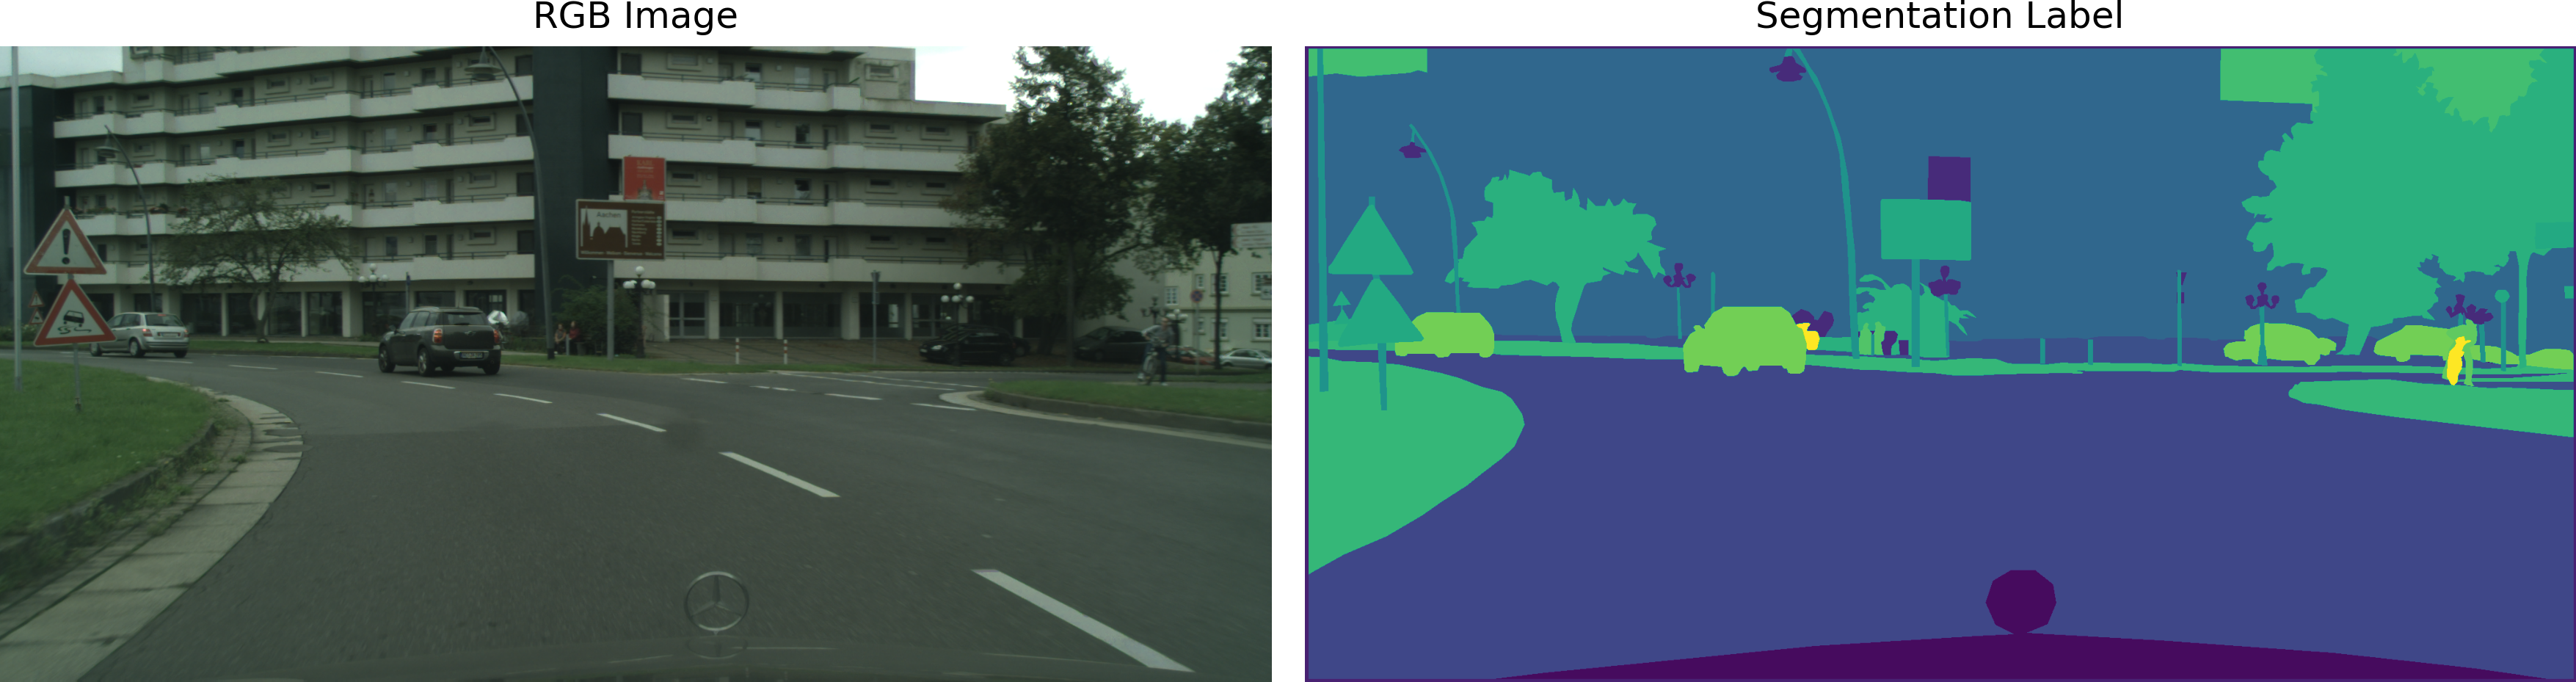
\includegraphics[scale=0.49]{pictures/output_plot_0.png}
        %    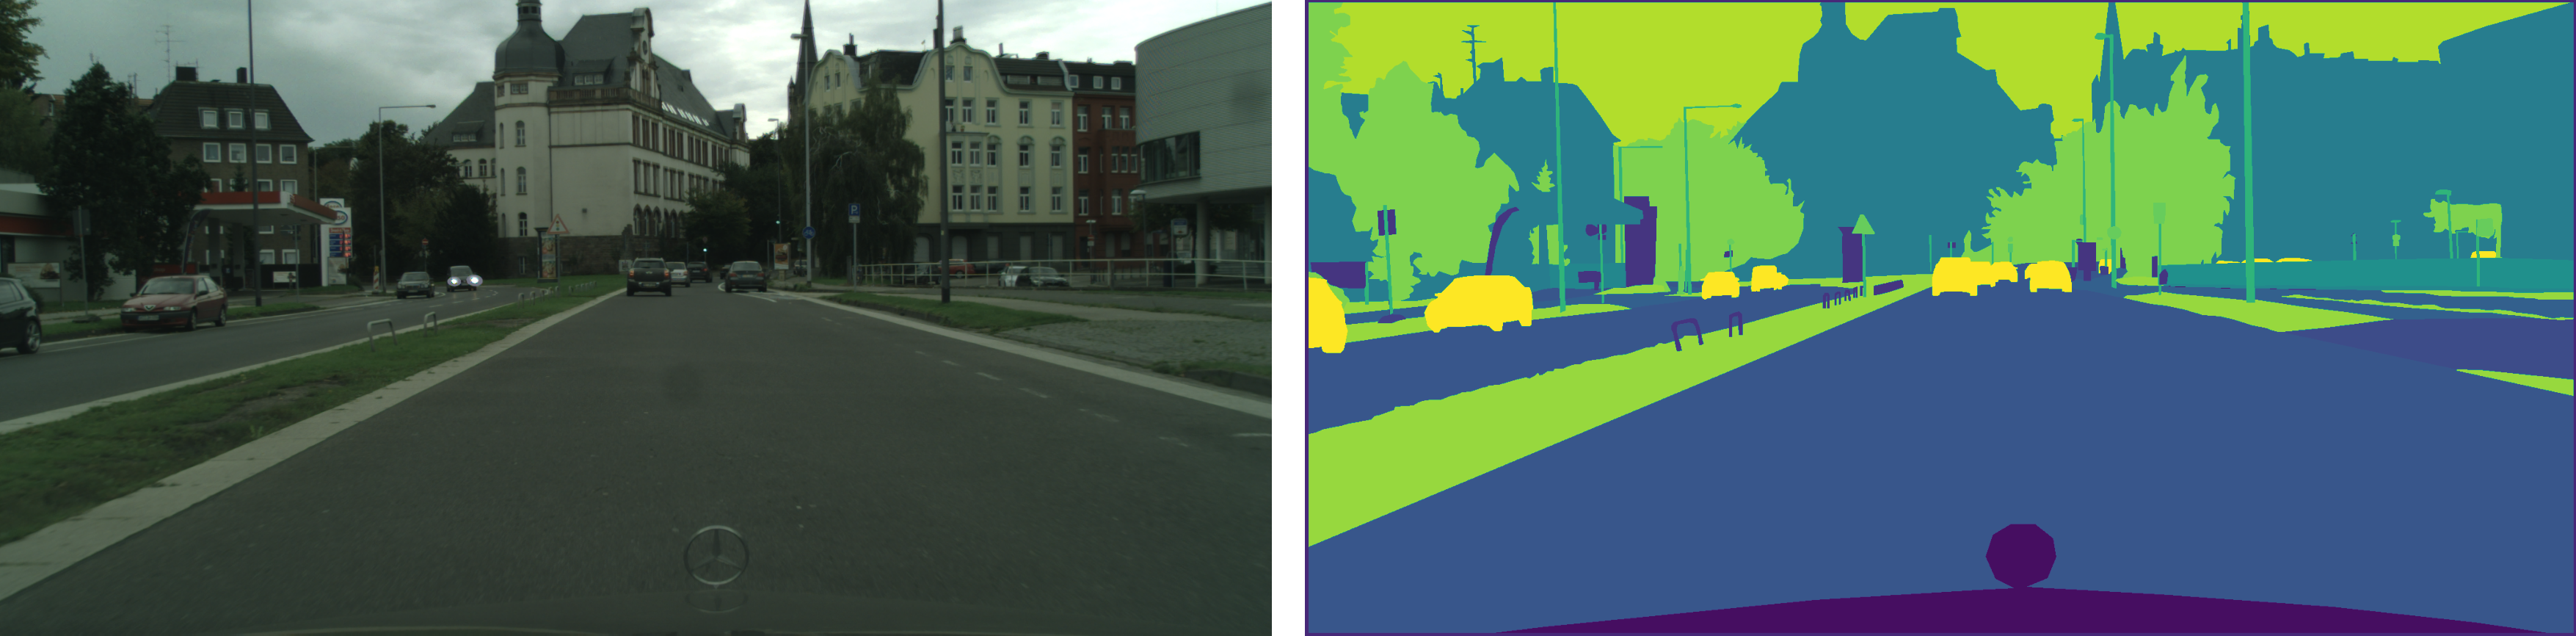
\includegraphics[scale=0.49]{pictures/output_plot_1.png}
        %    \caption{Die ersten zwei Bilder des Cityscapes Dataset aus Aachen.}
        %\end{figure}        
    
\newpage  
        \subsection{KI-rekonstruierte Bilder}
            Für die KI-rekonstruierten Bilder werden zwei VQ-VAE-Modelle verwendet, die in Kapitel 5 (Modelle) vorgestellt wurden. Anders als bei traditionellen Bildkompressionsverfahren wie JPEG wird das Bild in diesem Ansatz nicht nur komprimiert, sondern anschließend rekonstruiert. Daraus entstanden zwei neue Datensätze, die für die weiteren Untersuchungen erstellt wurden.
            
            Die beiden KI-Datensätze werden sowohl untereinander als auch zu den Originaldaten sowie zu den JPEG-Daten mithilfe der drei Metriken SSIM, PSNR und MSE untersucht.
            Anders als bei der Untersuchung von JPEG werden hier die Metriken nicht in Abhängigkeit von der Kompressionsqualität gemessen, da sich diese ausschließlich auf die JPEG-Komprimierung bezieht.
            Für den Vergleich und die Untersuchung der KI-rekonstruierten Datensätze werden die Metriken stattdessen in Abhängigkeit vom Kompressionsfaktor gemessen.

            In Abbildung \ref{fig:speicher_kompressionsfaktor} ist der Kompressionsfaktor der einzelnen
            JPEG-Datensätze in Bezug auf ihre Kompressionsqualität dargestellt. Die Kurve ist nicht linear und zeigt einen maximalen Kompressionsfaktor von $56,33$ bei einer Kompressionsqualität von $5\%$.
            Im Vergleich dazu erreichen die beiden Modelle deutlich höhere Kompressionsfaktoren.
            \begin{itemize}
                \item \textbf{vq-f16} f=16, VQ (Z=16384, d=8)\\
                    Erreicht einen Kompressionsfaktor von $219,43$
                \item \textbf{vq-f8-n256} f=8, VQ (Z=256, d=4)\\
                     Erreicht einen Kompressionsfaktor von $192$
            \end{itemize}
            Obwohl das Codebuch des \textbf{vq-f8-n256} signifikant kleiner ist und weniger Einträge enthält, um die latenten Vektoren auf die Codebuchvektoren abzubilden, und die Dimension der latenten Vektoren mit $d = 4$ ebenfalls geringer ist, erzielt das \textbf{vq-f8-n256}-Modell eine niedrigere Kompression.
            Die Zerlegung des Bildes erfolgt durch kleinere Blöcke, was einen stärkeren Einfluss darauf hat, wie stark die Kompression letztendlich ausfällt. Da die Blöcke der Größe $f \times f$ auf die Höhe und die Breite des Bildes angewandt werden, ist der Wert $f$ vierfach zu zählen im Vergleich zur Dimension $d$.
            Das bedeutet, dass für ($f = 8$, $d=4$) der gleiche latente Vektor wie für ($f=16$, $d=8$) erst dann resultieren würde, wenn ($f=8$, $d=2$) verwendet wird.

\newpage 
            \underline{\textbf{Qualität der Bilder}}\bigskip
\begin{comment}         
            Original im Vergleich zum \textbf{vq-f16} Modell      
            \begin{figure}[!htb]
                \centering
                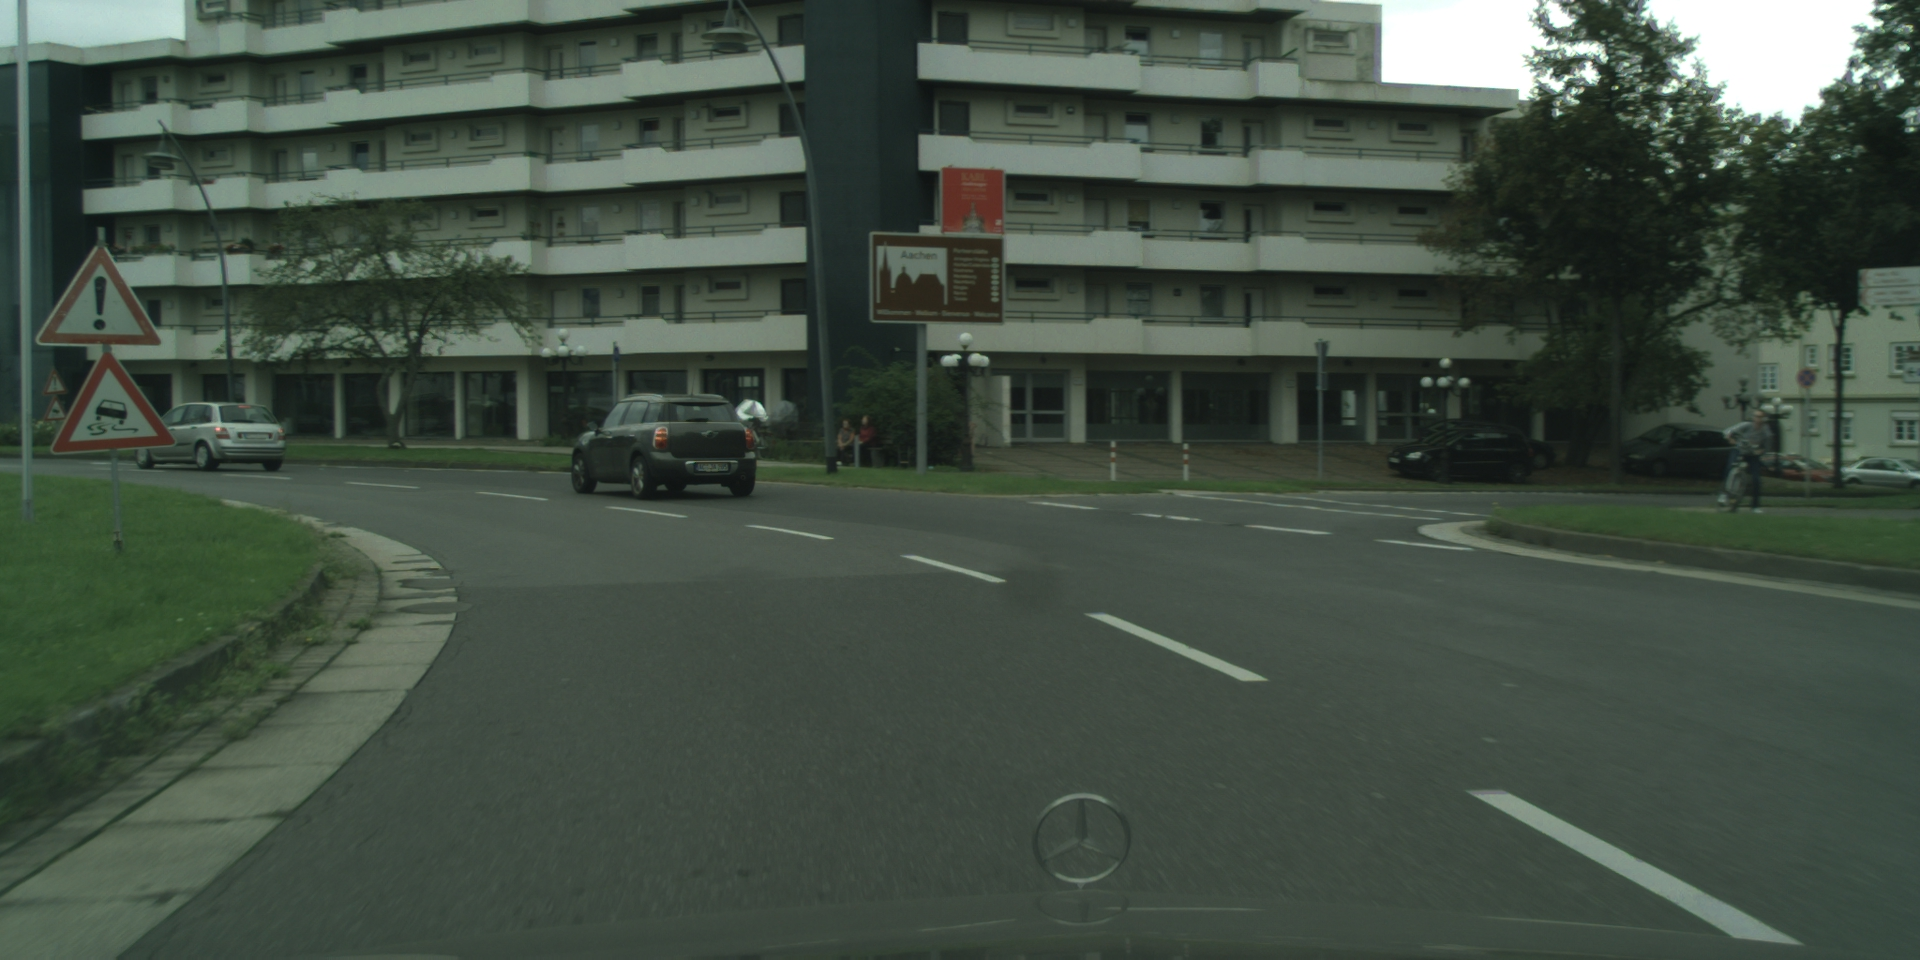
\includegraphics[scale=0.19]{pictures/img00_png.png}
                \caption{Originales Bild aus dem Cityscapes  Datensatz (Aachen erstes Bild).}
                \label{fig:og0_aachen_000000}
            \end{figure}
            \begin{figure}[!htb]
                \centering
                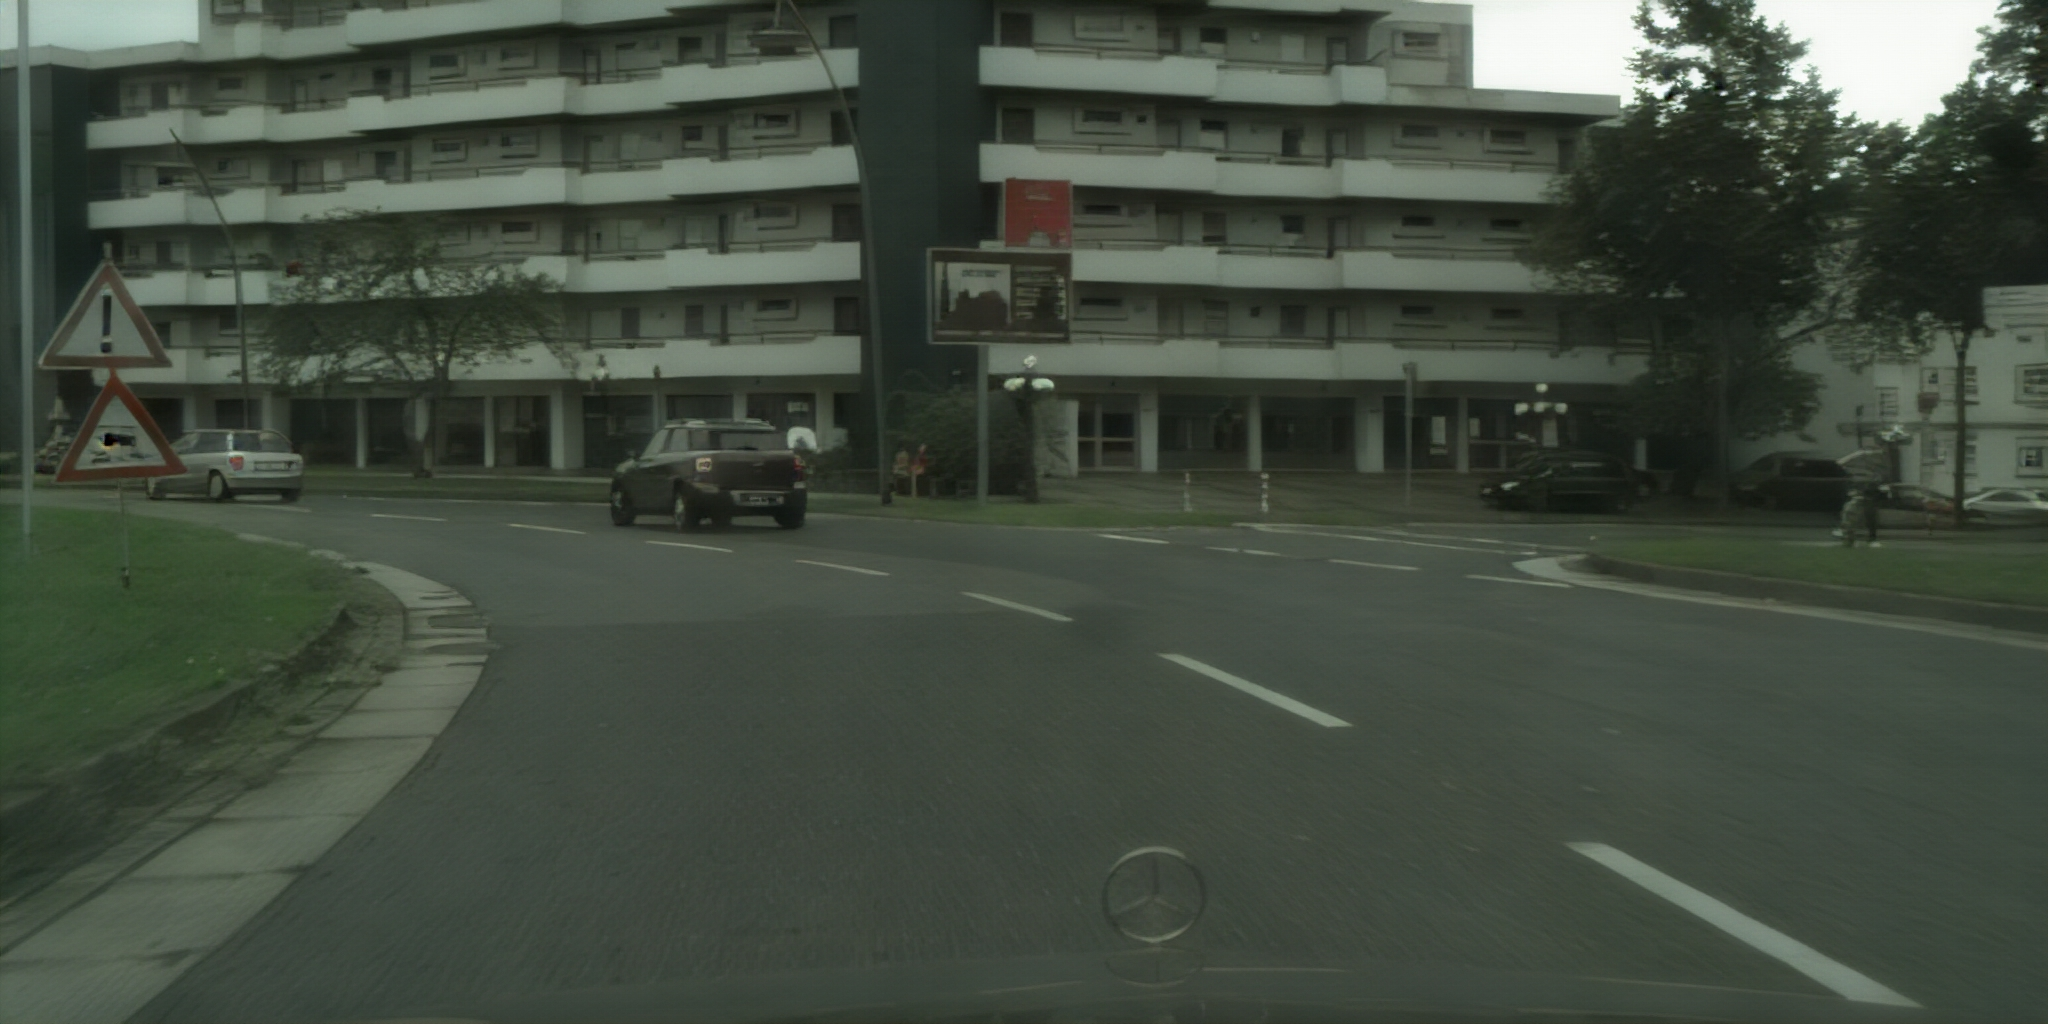
\includegraphics[scale=0.19]{pictures/img00_vq-f16.png}
                \caption{Rekonstruiertes Bild mit vq-f16 Modell (Aachen erstes Bild).}
                \label{fig:0_vq-f16_aachen_000000}
            \end{figure}

\newpage
            Original im Vergleich zum \textbf{vq-f8-n256} Modell      
            \begin{figure}[!htb]
                \centering
                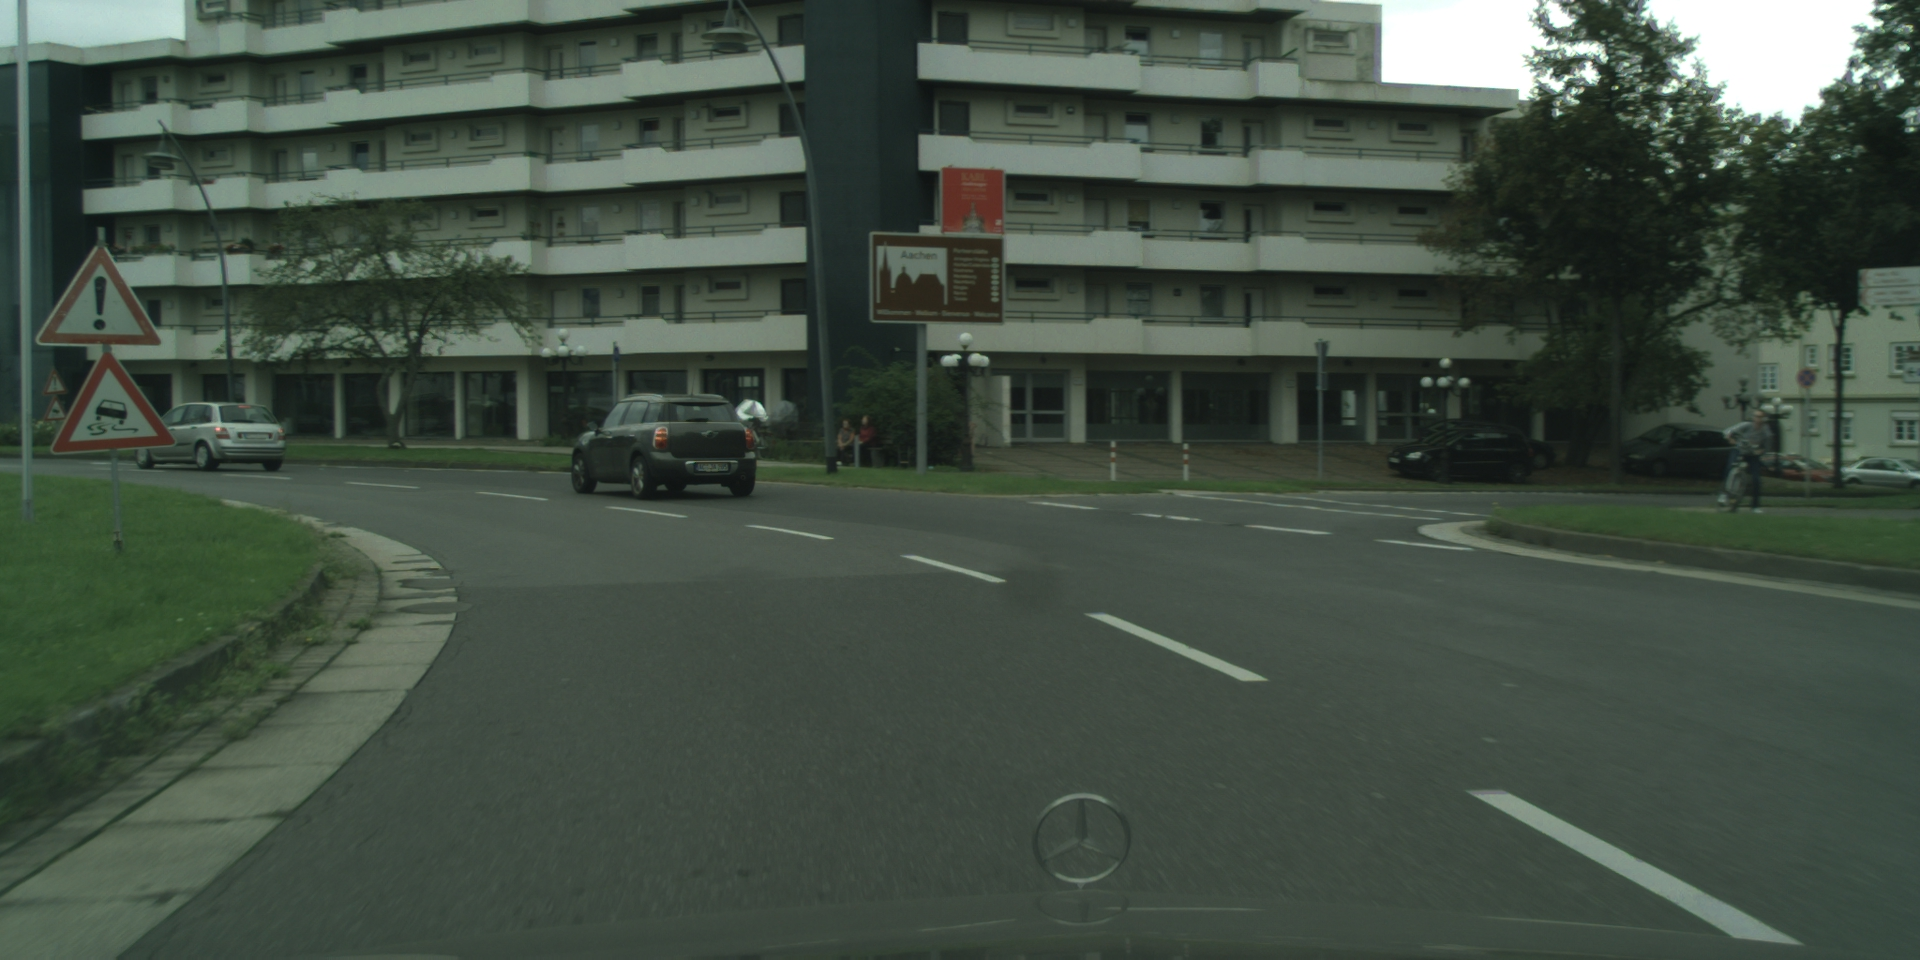
\includegraphics[scale=0.19]{pictures/img00_png.png}
                \caption{Originales Bild aus dem Cityscapes  Datensatz (Aachen erstes Bild).}
                \label{fig:og1_aachen_000000}
            \end{figure}
            \begin{figure}[!htb]
                \centering
                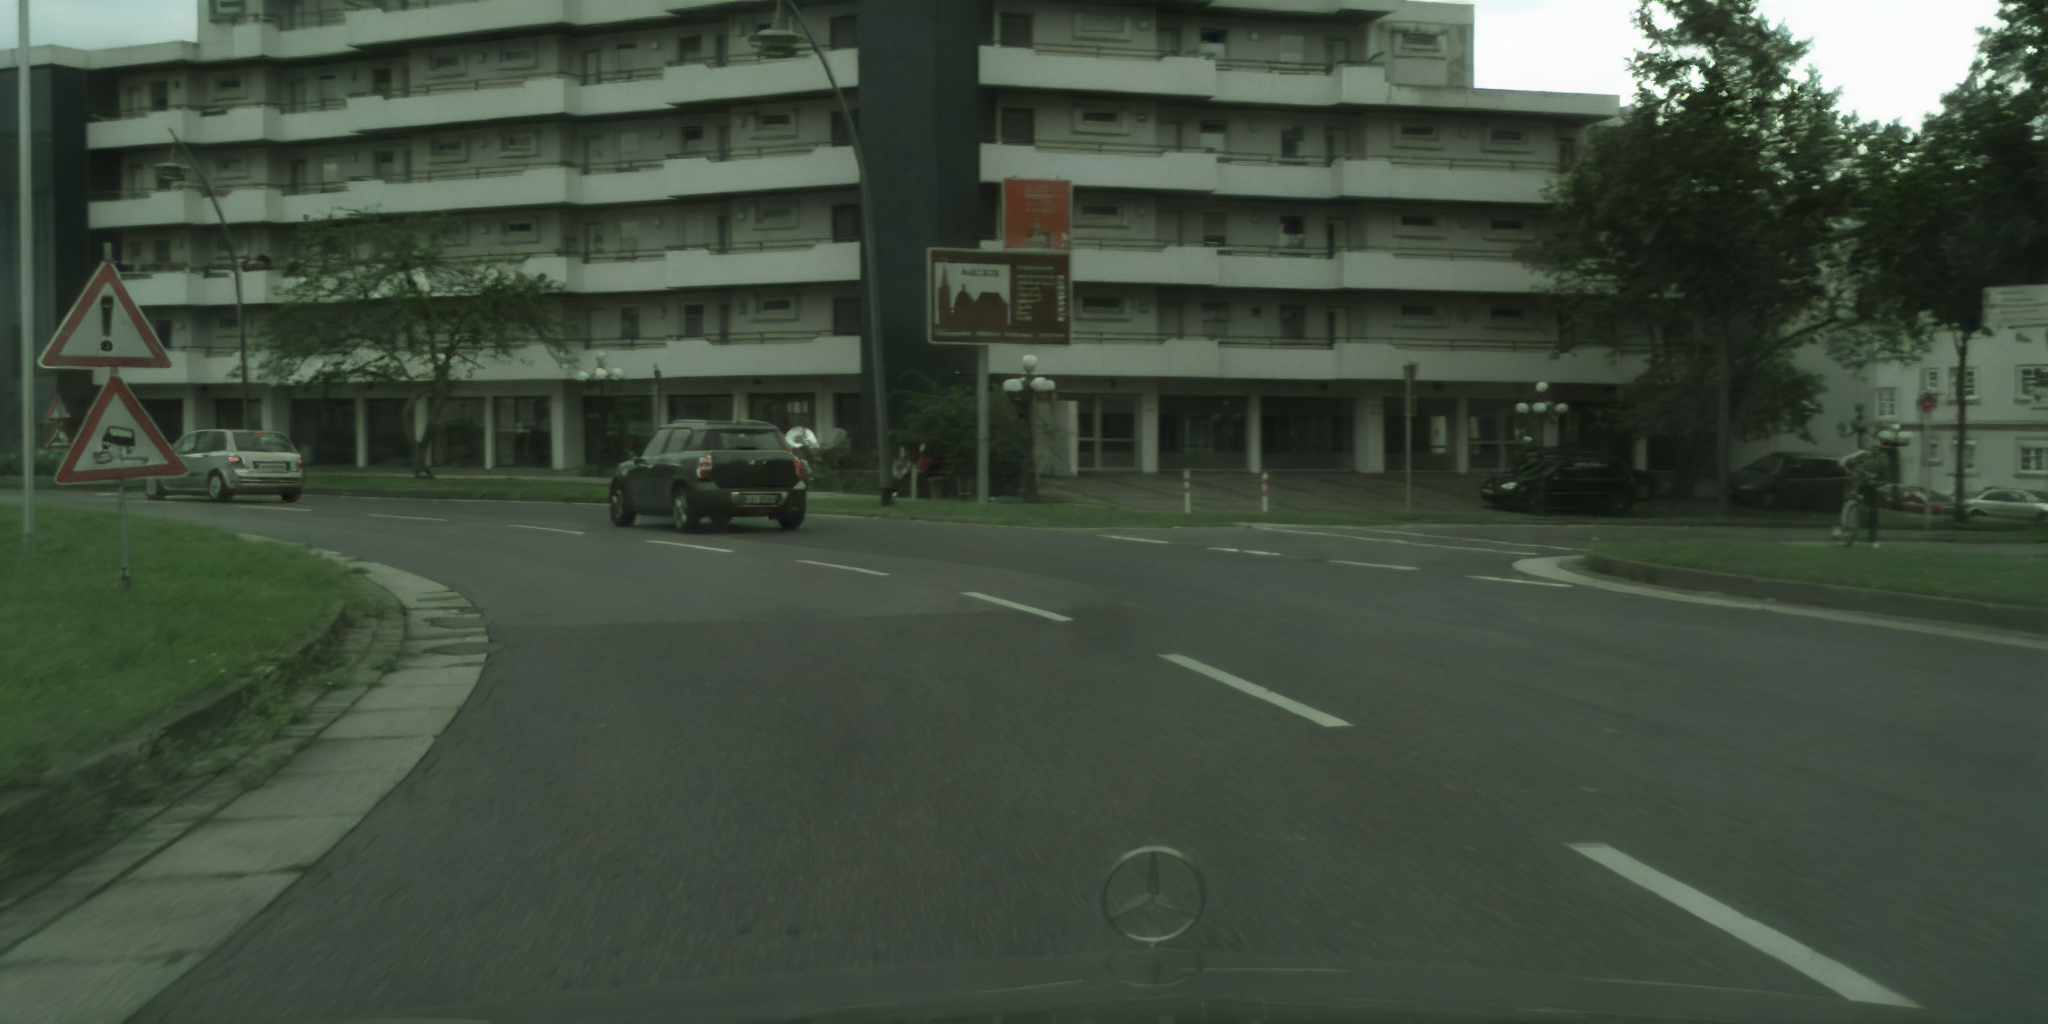
\includegraphics[scale=0.19]{pictures/img00_vq-f8-n256.png}
                \caption{Rekonstruiertes Bild mit vq-f8-n256 Modell (Aachen erstes Bild).}
                \label{fig:0_vq-f8-n256_aachen_000000}
            \end{figure}

\newpage
            \textbf{vq-f16} im Vergleich zu \textbf{vq-f8-n256} rekonstruierten Bild
\end{comment}
            \begin{figure}[!htb]
                \centering
                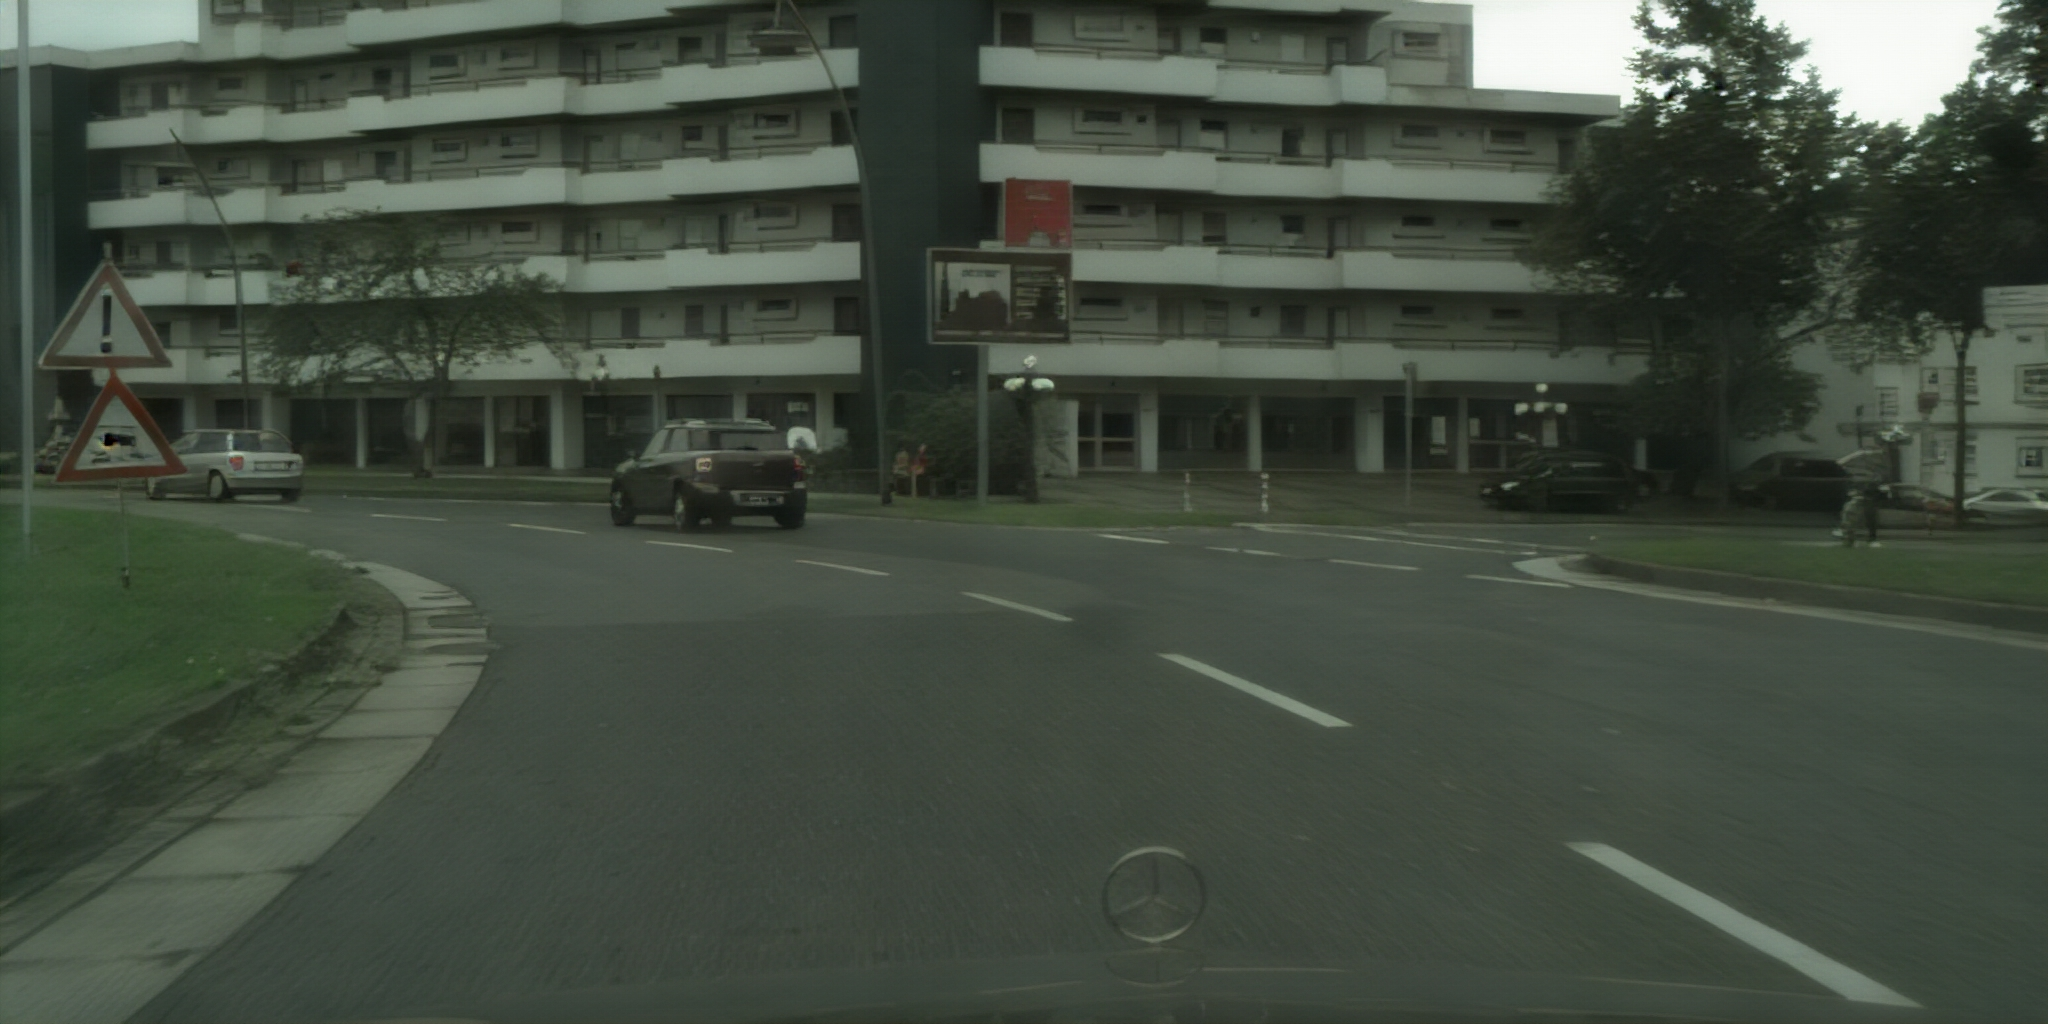
\includegraphics[scale=0.19]{pictures/img00_vq-f16.jpg}
                \caption{Rekonstruiertes Bild mit vq-f16 Modell (Aachen erstes Bild).}
                \label{fig:1_vq-f16_aachen_000000}
            \end{figure}
            \begin{figure}[!htb]
                \centering
                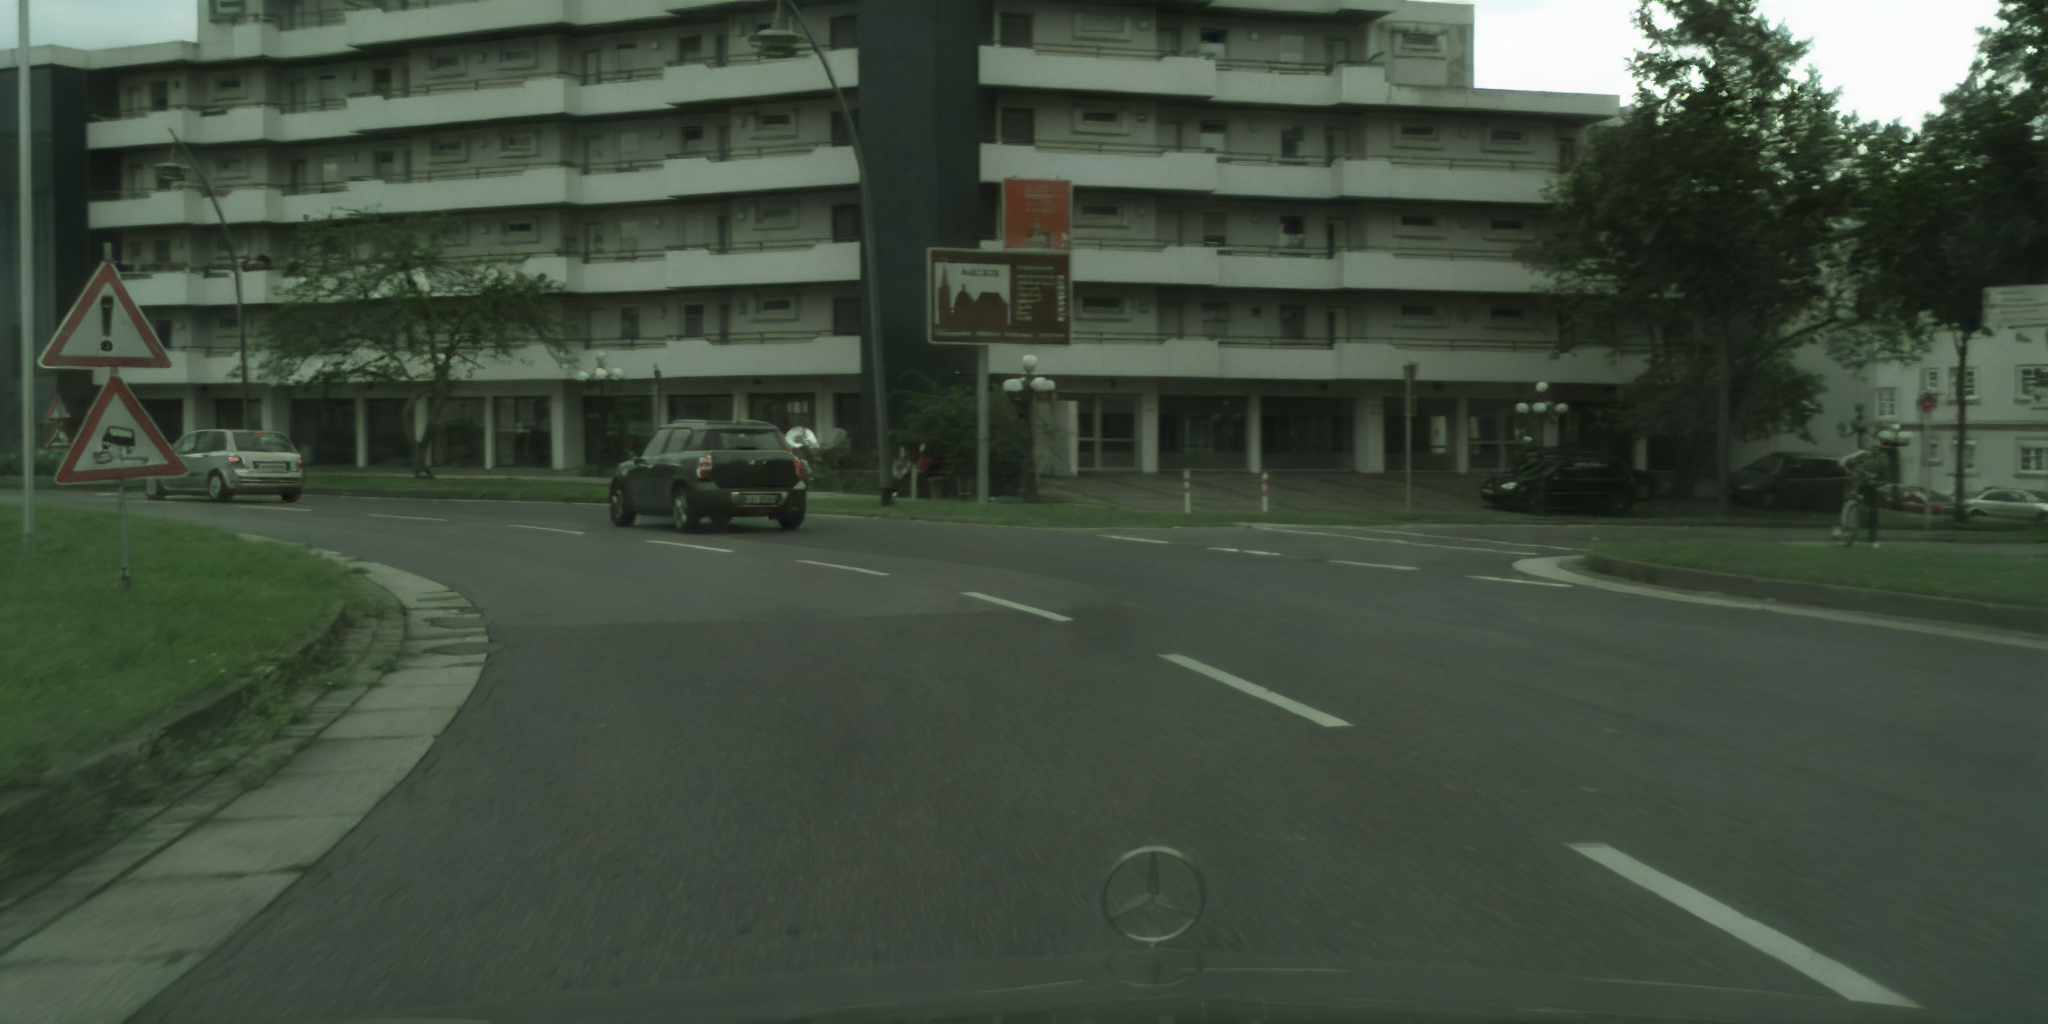
\includegraphics[scale=0.19]{pictures/img00_vq-f8-n256.jpg}
                \caption{Rekonstruiertes Bild mit vq-f8-n256 Modell (Aachen erstes Bild).}
                \label{fig:1_vq-f8-n256_aachen_000000}
            \end{figure}
            
\newpage  
            \begin{figure}[!htb]
                \centering
                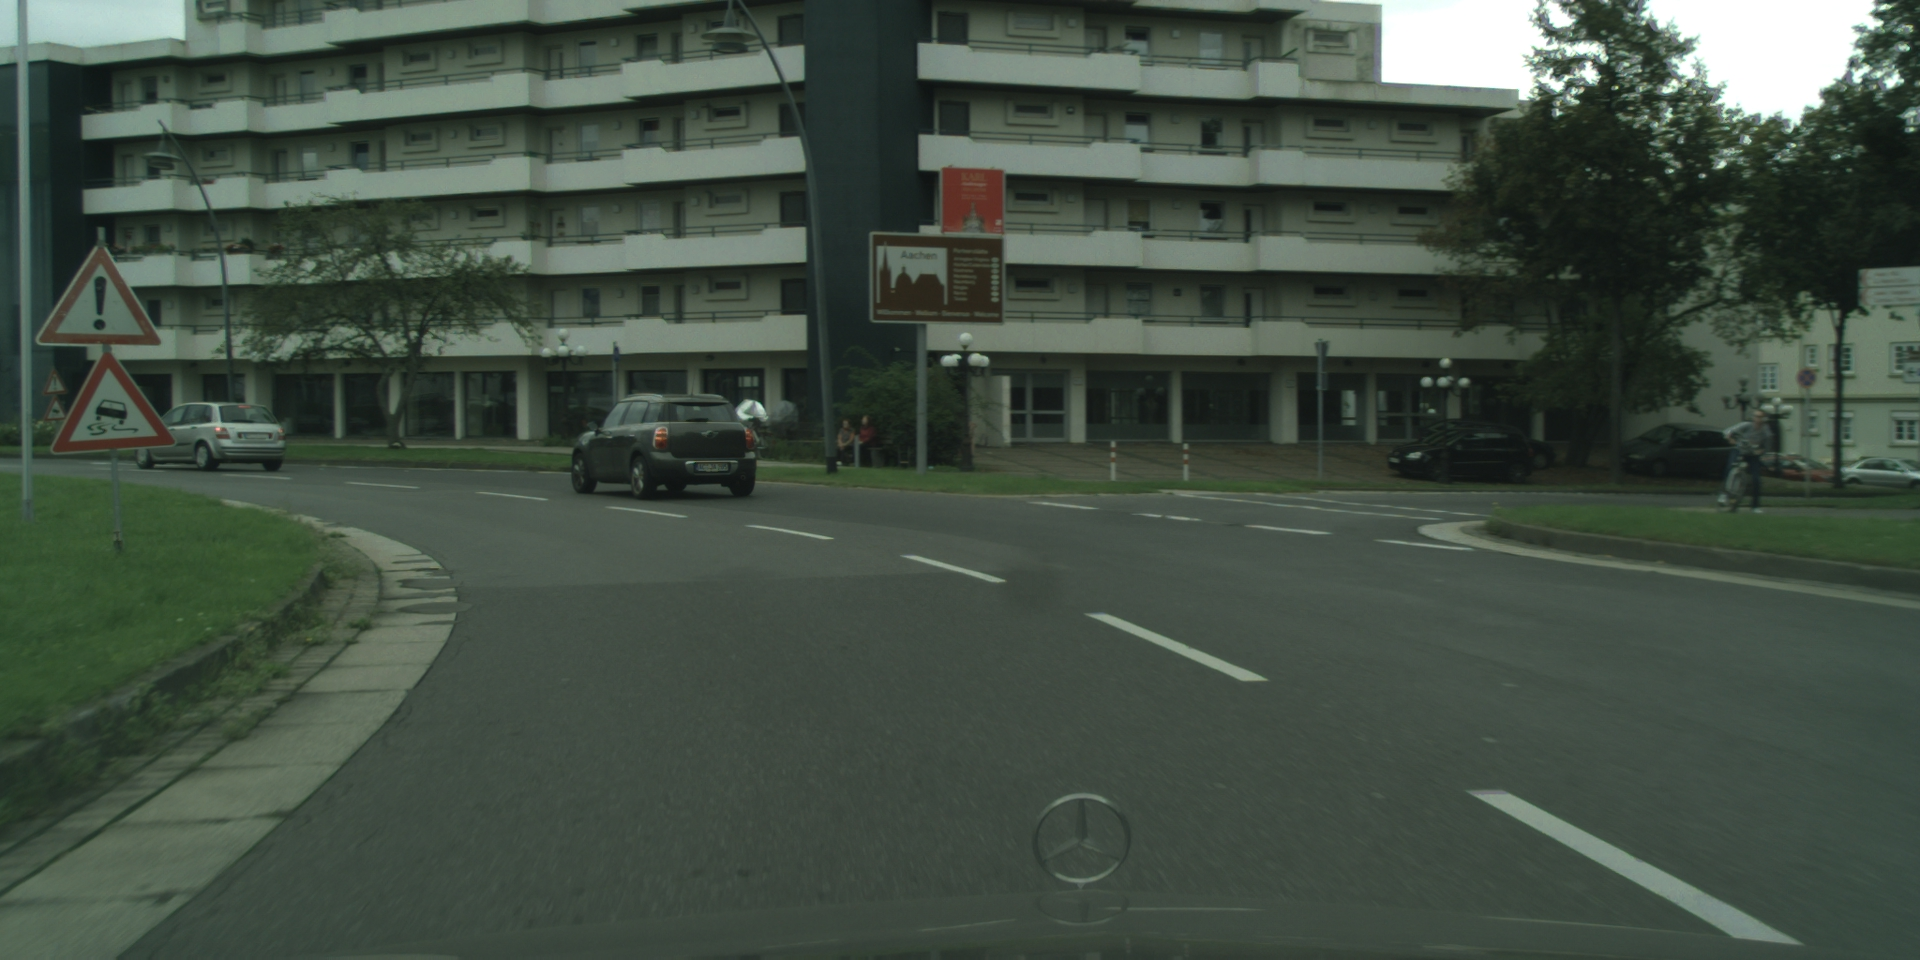
\includegraphics[scale=0.19]{pictures/img00_png.jpg}
                \caption{Originales Bild aus dem Cityscapes  Datensatz (Aachen erstes Bild).}
                \label{fig:og1_aachen_000000}
            \end{figure}
            Zwischen dem Originalbild und dem \textbf{vq-f16}-rekonstruierten Bild sind bei der Stärke der Kompression kaum oder nur geringe Veränderungen sichtbar.
            Dennoch sind Unterschiede in Farbe und Kontrast erkennbar. Auch Details wurden nicht mehr so präzise rekonstruiert. Das Nummernschild des Autos oder das Straßenschild zeigen eindeutig, dass das Bild nicht echt ist. Betrachtet man nun das Bild, welches das \textbf{vq-f8-n256}-Modell rekonstruiert hat, so ist es dem Original noch näher. Details, wie sie auf dem Schild zu erkennen sind, sind deutlich besser als bei dem Bild, welches das \textbf{vq-f16}-Modell erstellt hat. Obwohl der Kompressionsfaktor lediglich eine Differenz von $219,43 - 192 = 27,43$ aufweist, sind die Details der beiden modellbasiert rekonstruierten Bilder sehr unterschiedlich. Das Bild des \textbf{vq-f8-n256}-Modells ist für das menschliche Auge, was die Unterschiede zum Original betrifft, nur bei genauerer Betrachtung erkennbar. Selbst ein direkter Vergleich mit dem Original zeigt nicht auf Anhieb, dass es sich um zwei verschiedene Bilder handelt.

\newpage
            \begin{figure}[!htb]
                \centering
                \includesvg[scale=0.56]{graphs/output_plot_mse_model.svg}
                \caption{MSE in Abhängigkeit zum Kompressionsfaktor. Vergleich zwischen JPEG-Kompression und KI-Modell rekonstruierter Bilder.}
                \label{fig:output_plot_mse_model}
            \end{figure}

            Es zeigt sich, dass der MSE des \textbf{vq-f16} ähnlich hoch ist wie der des JPEG-Datensatzes mit einer Kompressionsqualität von $5\%$, obwohl bei direktem Vergleich der Bilder mit bloßem Auge sofort erkennbar ist, dass ein deutlicher qualitativer Unterschied besteht.\\          
            
            \begin{figure}[!htb]
                \centering
                \begin{minipage}[!htb]{0.47\textwidth}
                    \centering
                    \textbf{Komprimiert ($5\%$)} % Überschrift für die erste Spalte
                \end{minipage}
                %
                \begin{minipage}[!htb]{0.47\textwidth}
                    \centering
                    \textbf{\textbf{vq-f16}} % Überschrift für die zweite Spalte
                \end{minipage}

                \begin{minipage}[!htb]{0.47\textwidth}
                    \centering
                    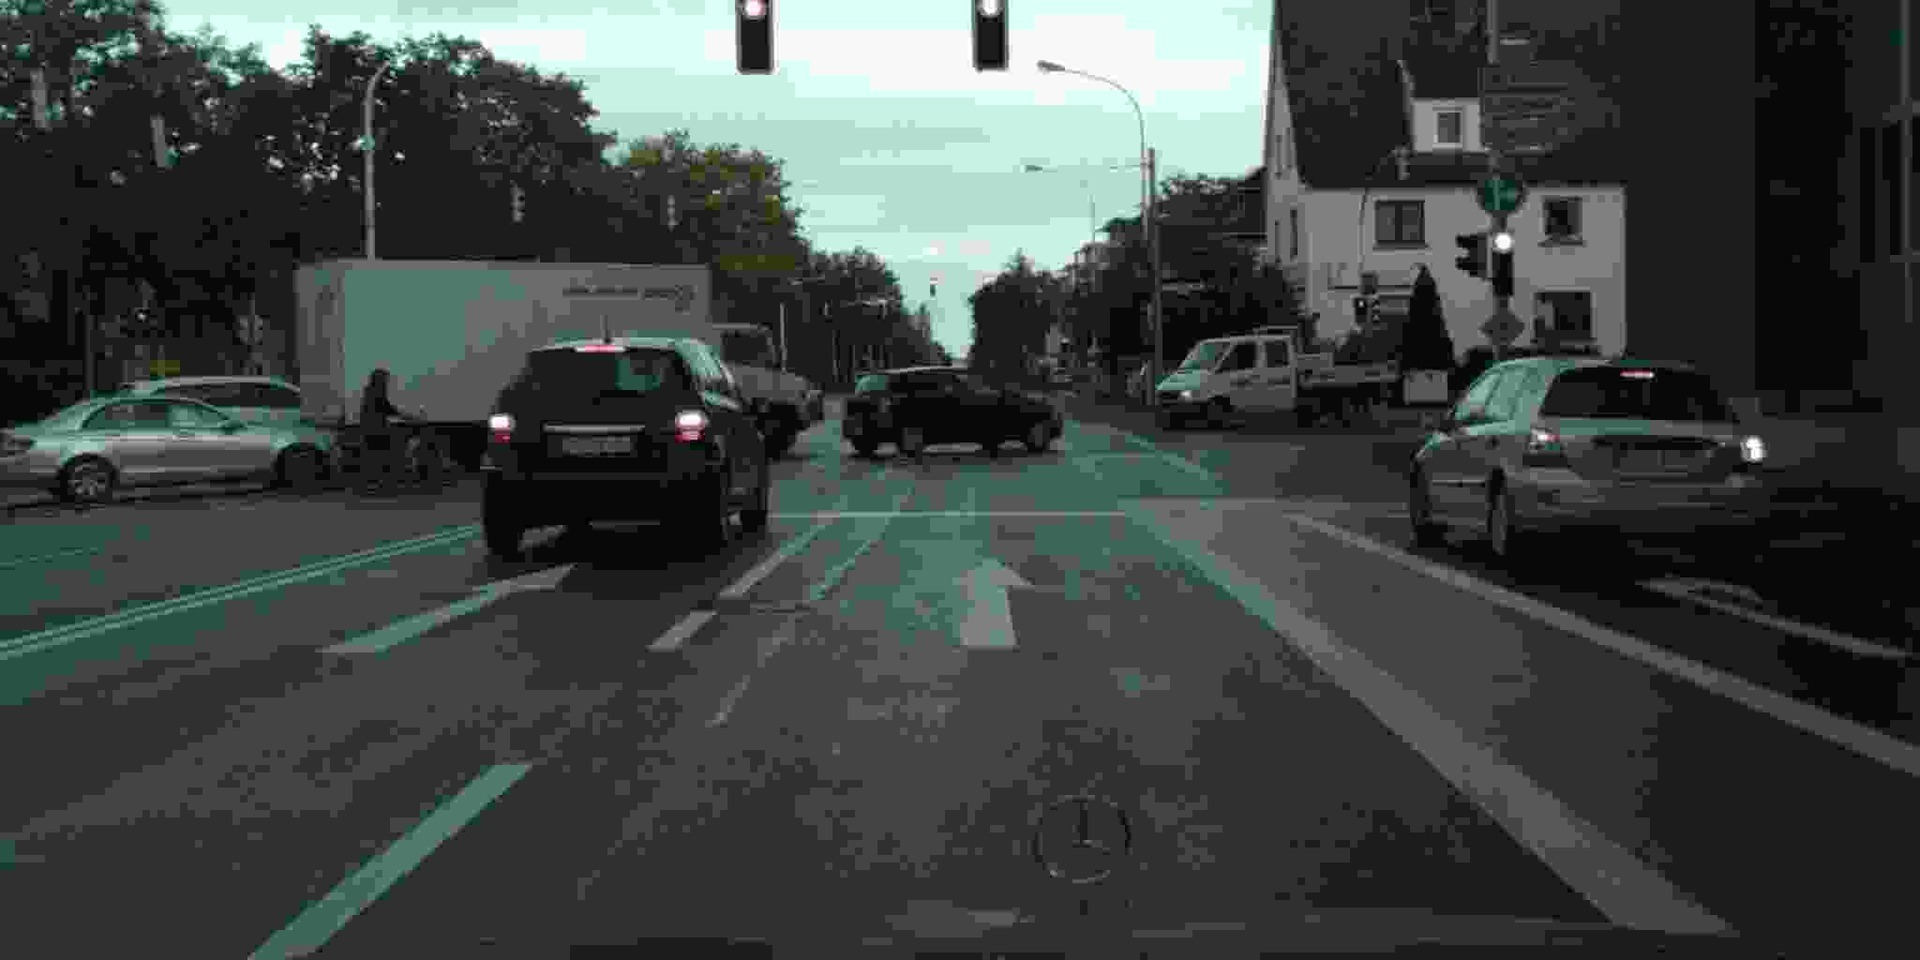
\includegraphics[width=\textwidth]{pictures/img_jpg5_darmstadt_000002.jpg}    
                    \label{fig:bild132}
                \end{minipage}
                %
                \begin{minipage}[!htb]{0.47\textwidth}
                    \centering
                    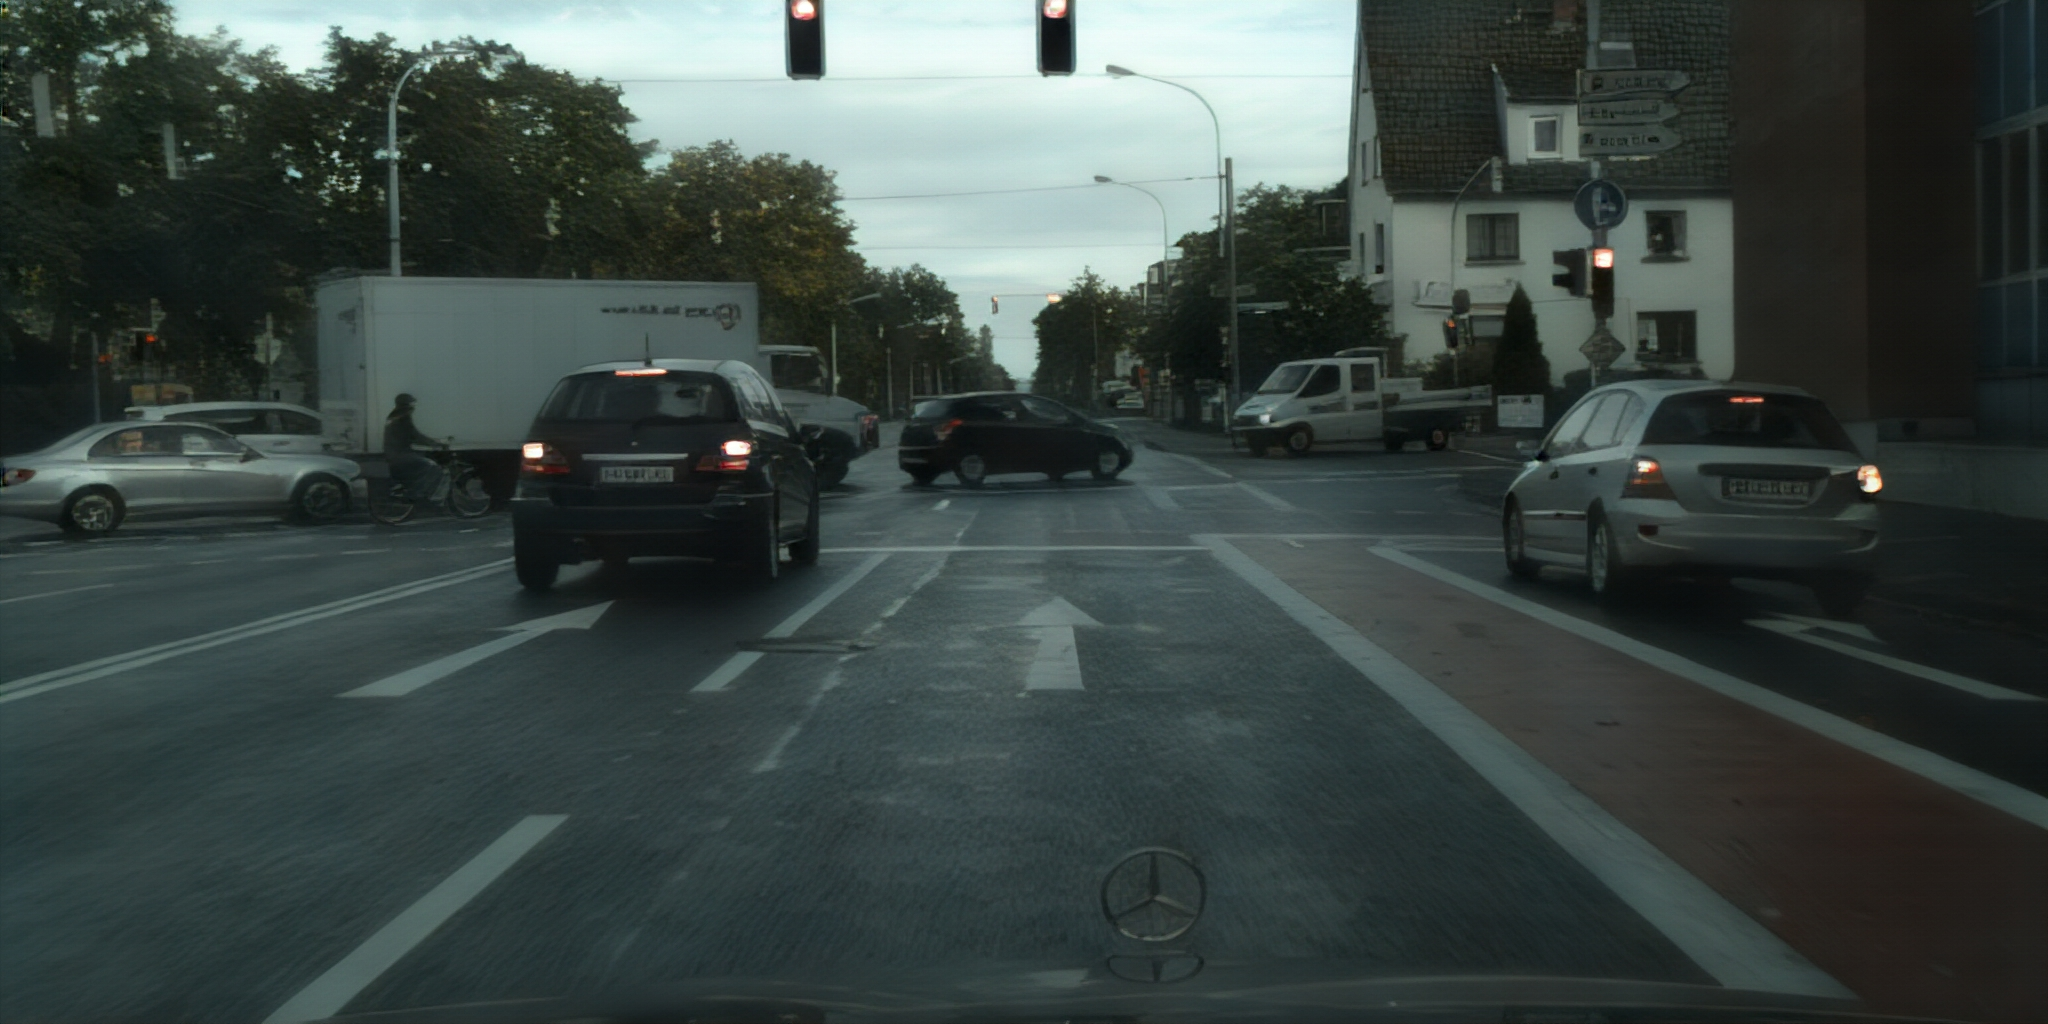
\includegraphics[width=\textwidth]{pictures/vq-f16_darmstadt_000002.jpg}
                    \label{fig:bild142}
                \end{minipage}
            \end{figure}

            Dies zeigt, dass der MSE nicht besonders gut geeignet ist, um die Qualität eines Bildes zu bestimmen. MSE sowie PSNR berücksichtigen nicht die menschliche Wahrnehmung des Auges, wie es der SSIM tut, was die Bewertung eines Bildes betrifft \cite{mse_psnr_eye}.
\newpage
            \begin{figure}[!htb]
                \centering
                \begin{minipage}[!htb]{0.47\textwidth}
                    \centering
                    \textbf{Komprimiert ($10\%$)} % Überschrift für die erste Spalte
                \end{minipage}
                %
                \begin{minipage}[!htb]{0.47\textwidth}
                    \centering
                    \textbf{\textbf{vq-f8-n256}} % Überschrift für die zweite Spalte
                \end{minipage}

                \begin{minipage}[!htb]{0.47\textwidth}
                    \centering
                    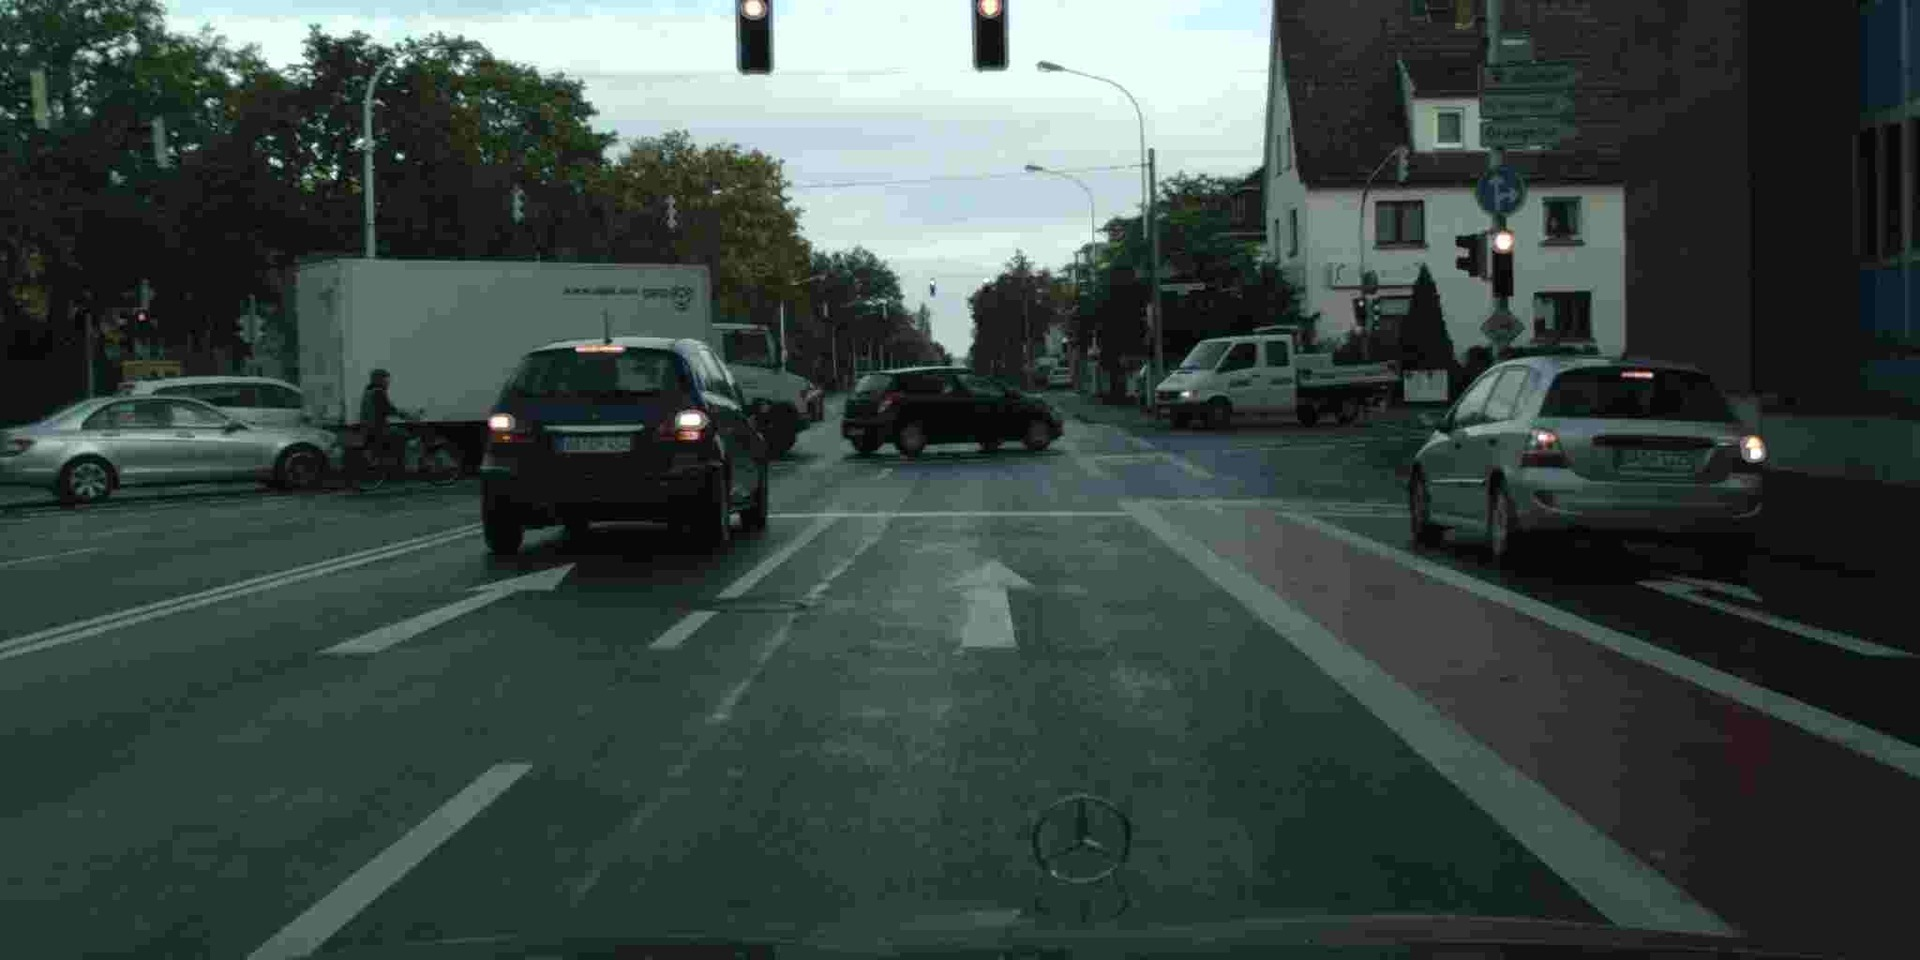
\includegraphics[width=\textwidth]{pictures/jpg10_darmstadt_000002.jpg}    
                \end{minipage}
                %
                \begin{minipage}[!htb]{0.47\textwidth}
                    \centering
                    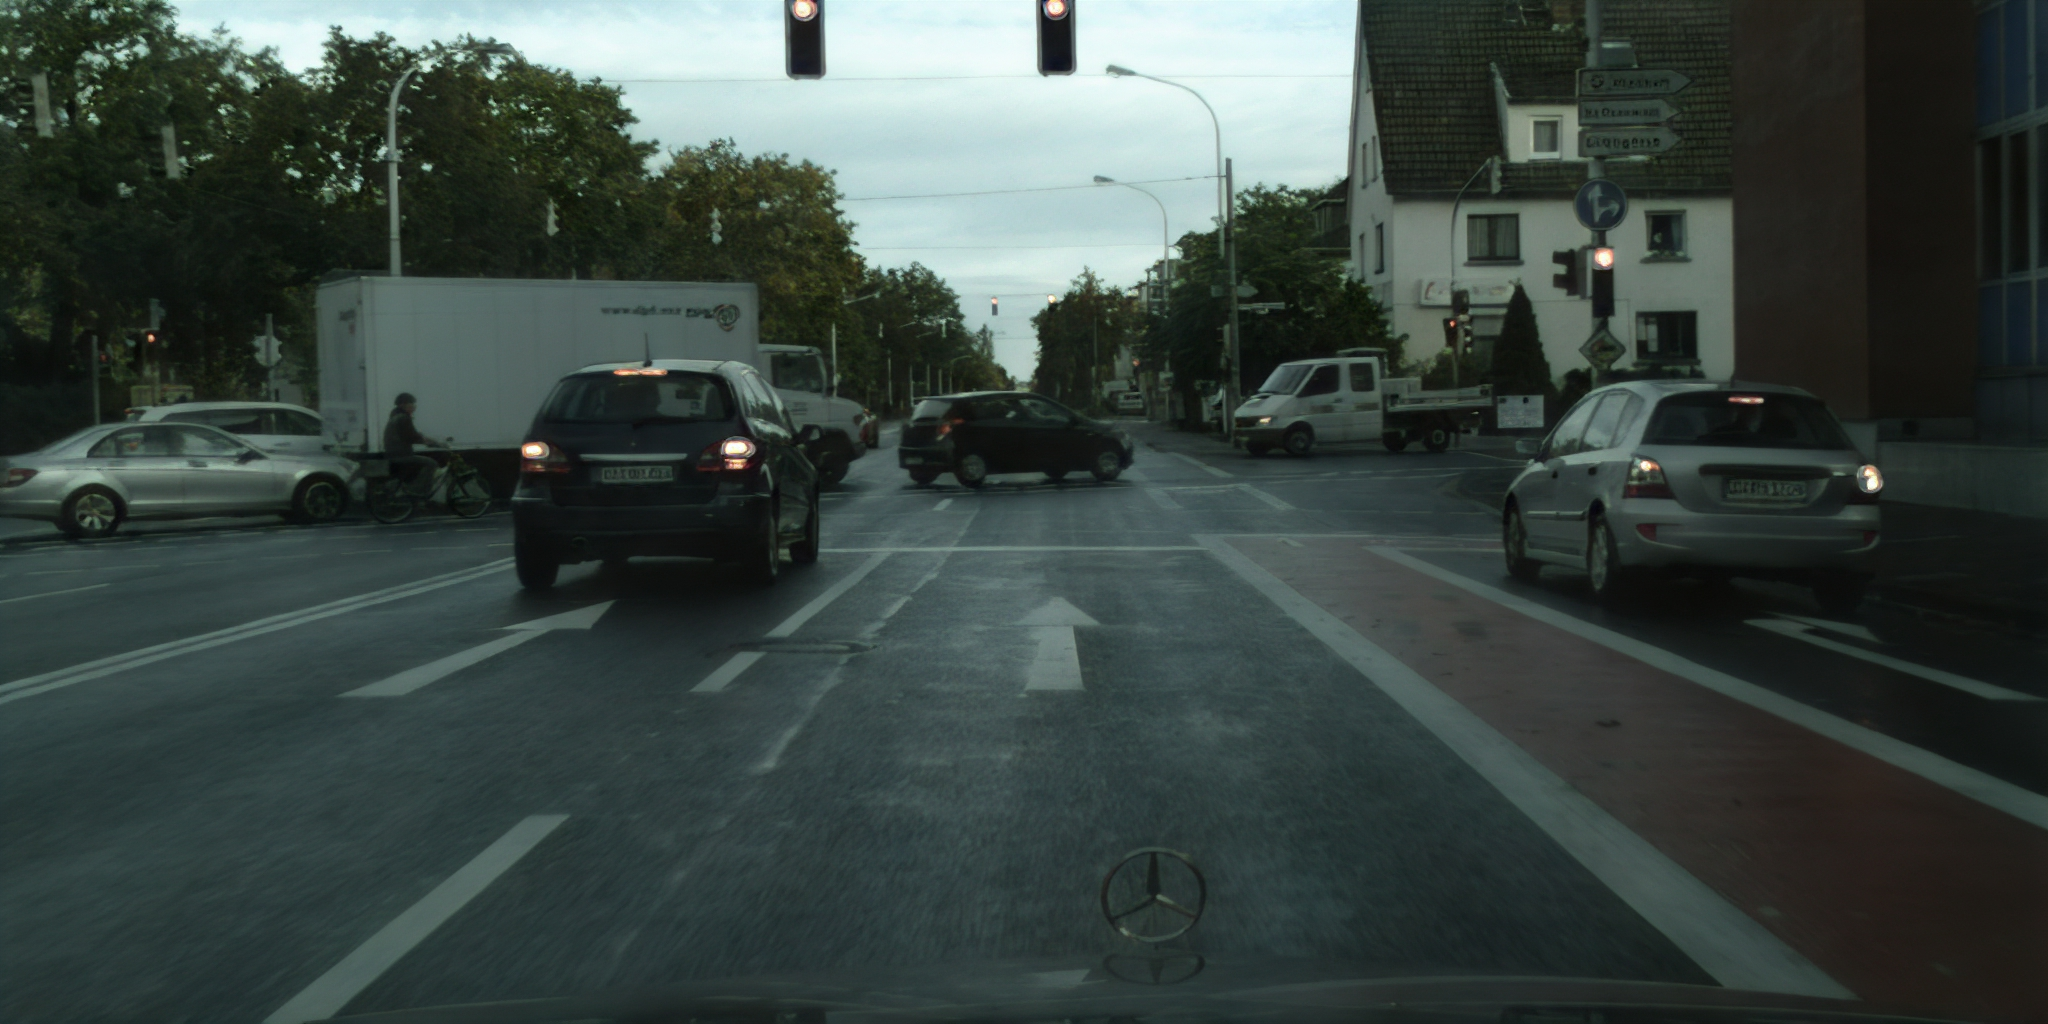
\includegraphics[width=\textwidth]{pictures/vq-f8-n256_darmstadt_000002.jpg}
                \end{minipage}
            \end{figure}

            Auch der MSE des \textbf{vq-f8-n256} ist mit $9,8e^{-4}$ hoch und größer als der der Bilder mit einer Kompressionsqualität von $10\%$ mit $8,07e^{-4}$. Der MSE ist somit kein Maßstab, mit dem sich Bilder gut auf ihre Qualität überprüfen lassen. Auch hier zeigt sich das, obwohl der MSE des \textbf{vq-f8-n256}-Modells schlechter ist, die Bilder jedoch qualitativ hochwertiger sind.

            \begin{figure}[!htb]
                \centering
                \includesvg[scale=0.56]{graphs/output_plot_psnr_model.svg}
                \caption{PSNR in Abhängigkeit zum Kompressionsfaktor. Vergleich zwischen JPEG-Kompression und KI-Modell rekonstruierter Bilder.}
                \label{fig:output_plot_psnr_model}
            \end{figure}

            Auch beim PSNR zeigen beide Modelle schlechte Ergebnisse, mit PSNR-Werten von $76,52$ für das \textbf{vq-f16}-Modell und $78,46$ für das \textbf{vq-f8-n256}-Modell. Auch hier liegen, wie bereits beim MSE, beide Modelle mit ihren Werten in Bezug auf die Qualität zwischen den JPEG-Datensätzen mit einer Kompressionsqualität von $5\%$ und $10\%$. Dies steht jedoch im Widerspruch zur Qualitätswahrnehmung des menschlichen Auges, wie im direkten Vergleich der Bilder sichtbar wird.
\newpage
            \begin{figure}[!htb]
                \centering
                \includesvg[scale=0.56]{graphs/output_plot_ssim_model.svg}
                \caption{SSIM in Abhängigkeit zum Kompressionsfaktor. Vergleich zwischen JPEG-Kompression und KI-Modell rekonstruierter Bilder.}
                \label{fig:output_plot_ssim_model}
            \end{figure}

            In der obigen Grafik werden die Datensätze der traditionellen Kompression und der beiden Modelle im Vergleich zum SSIM gegenübergestellt. Es ist direkt erkennbar, dass die beiden Modelle deutlich besser abschneiden als bei MSE und PSNR. Beim SSIM liegen die beiden Modelle nicht zwischen den Datensätzen mit $5\%$ und $10\%$ Kompressionsqualität, was einem Wertebereich von $63,45 - 80,07$ entsprechen würde. Das \textbf{vq-f16}-Modell erzielt einen SSIM-Wert von $87,69$, während das \textbf{vq-f8-n256}-Modell mit einem Wert von $90,2$ abschneidet. Das \textbf{vq-f8-n256}-Modell erreicht somit sogar einen Wert, der zwischen den Datensätzen der Kompressionsqualität von $15\%$ und $20\%$ liegt.
            Dies zeigt, dass der SSIM für die Beschreibung der Bildqualität eindeutig besser geeignet ist, da er Helligkeit, Kontrast und Struktur berücksichtigt.
            
            Die Qualitätsdifferenz der beiden Modelle untereinander ist bei SSIM und PSNR geringer mit $3\%$ Unterschied, bei MSE weisen die beiden Modelle eine Differenz von $37\%$ auf.
            Die beiden Modelle schneiden im Vergleich zueinander ähnlich ab bei SSIM sowie bei PSNR, bei MSE 
            gibt es zwischen den Modellen jedoch eine große Lücke.
            
\newpage
    \section{Performance der Objektdetektion}
        Die einzelnen Datensätze sind hinsichtlich ihrer Kompression und Qualität durch Metriken wie SSIM, PSNR und MSE untersucht. Der nächste Schritt dieser Arbeit besteht darin, die einzelnen Datensätze in ein KI-Modell zu überführen. \\
        Ziel ist es, Boundingboxen um Objekte zu erzeugen und die Auswirkungen unterschiedlicher Kompressionsqualitäten sowie Kompressionsfaktoren auf die Objektdetektion zu messen. Der Originaldatensatz wird ebenfalls mit Boundingboxen versehen und dient als Referenz, wobei die Ground-Truth-Boundingboxen als Label verwendet werden.
        Dies ist notwendig, da die Boundingboxen des Cityscapes-Datensatzes mit einem anderen Modell erstellt wurden. Es werden jedoch die gleichen Grundvoraussetzungen benötigt, d.h. die Labels und die Datensätze, die für die Objekterkennung verwendet werden, müssen mit demselben Modell erstellt worden sein für gleiche Bedingungen, um miteinander verglichen werden zu können.
    
        Als Modell wurde ein vortrainiertes Netz von Ultralytics YOLO verwendet. Das YOLO-Modell (You Only Look Once), ein bedeutender Ansatz für Objekterkennung und Bildsegmentierung, wurde von Joseph Redmon und Ali Farhadi an der University of Washington entwickelt. Seit seiner Einführung im Jahr 2015 hat YOLO durch seine herausragende Kombination aus Geschwindigkeit und Präzision schnell an Popularität gewonnen.
        Das YOLO11-Modell, welches im Rahmen dieser Untersuchung verwendet wurde, ist zum Stand dieser Arbeit das neueste und State-of-the-Art-Modell von YOLO. Es wurde auf dem COCO-Datensatz trainiert und ist laut Angaben der Entwickler für Objekterkennung, Instanzsegmentierung, Bildklassifikation, Pose-Schätzung und die Erkennung orientierter Objekte (OBB) geeignet \cite{yolo_modell}.

        Der Originaldatensatz wurde mithilfe des Modells verarbeitet, und es wurden Boundingboxen um erkannte Objekte gelegt. Dieser neue Datensatz, der dadurch entstand, dient als Ground-Truth-Label-Datensatz für die weiteren Untersuchungen (siehe Kapitel 4, Konzept).

\newpage
        Zwei Label Bilder, welche das YOLO-Modell erzeugt hat, aus dem Originaldatensatz.
        Zu erkennen sind die Ground-Truth-Boundingboxen, farblich gekennzeichnet, abhängig von der Klasse.
        Die Zahl gibt den prozentualen Wert an, wie sicher sich das Modell dabei ist. Dieser spielt aber keine Rolle, da es sich hier um die generierten Ground-Truth-Boundingboxen handelt.
    
        \begin{figure}[!htb]
            \centering
            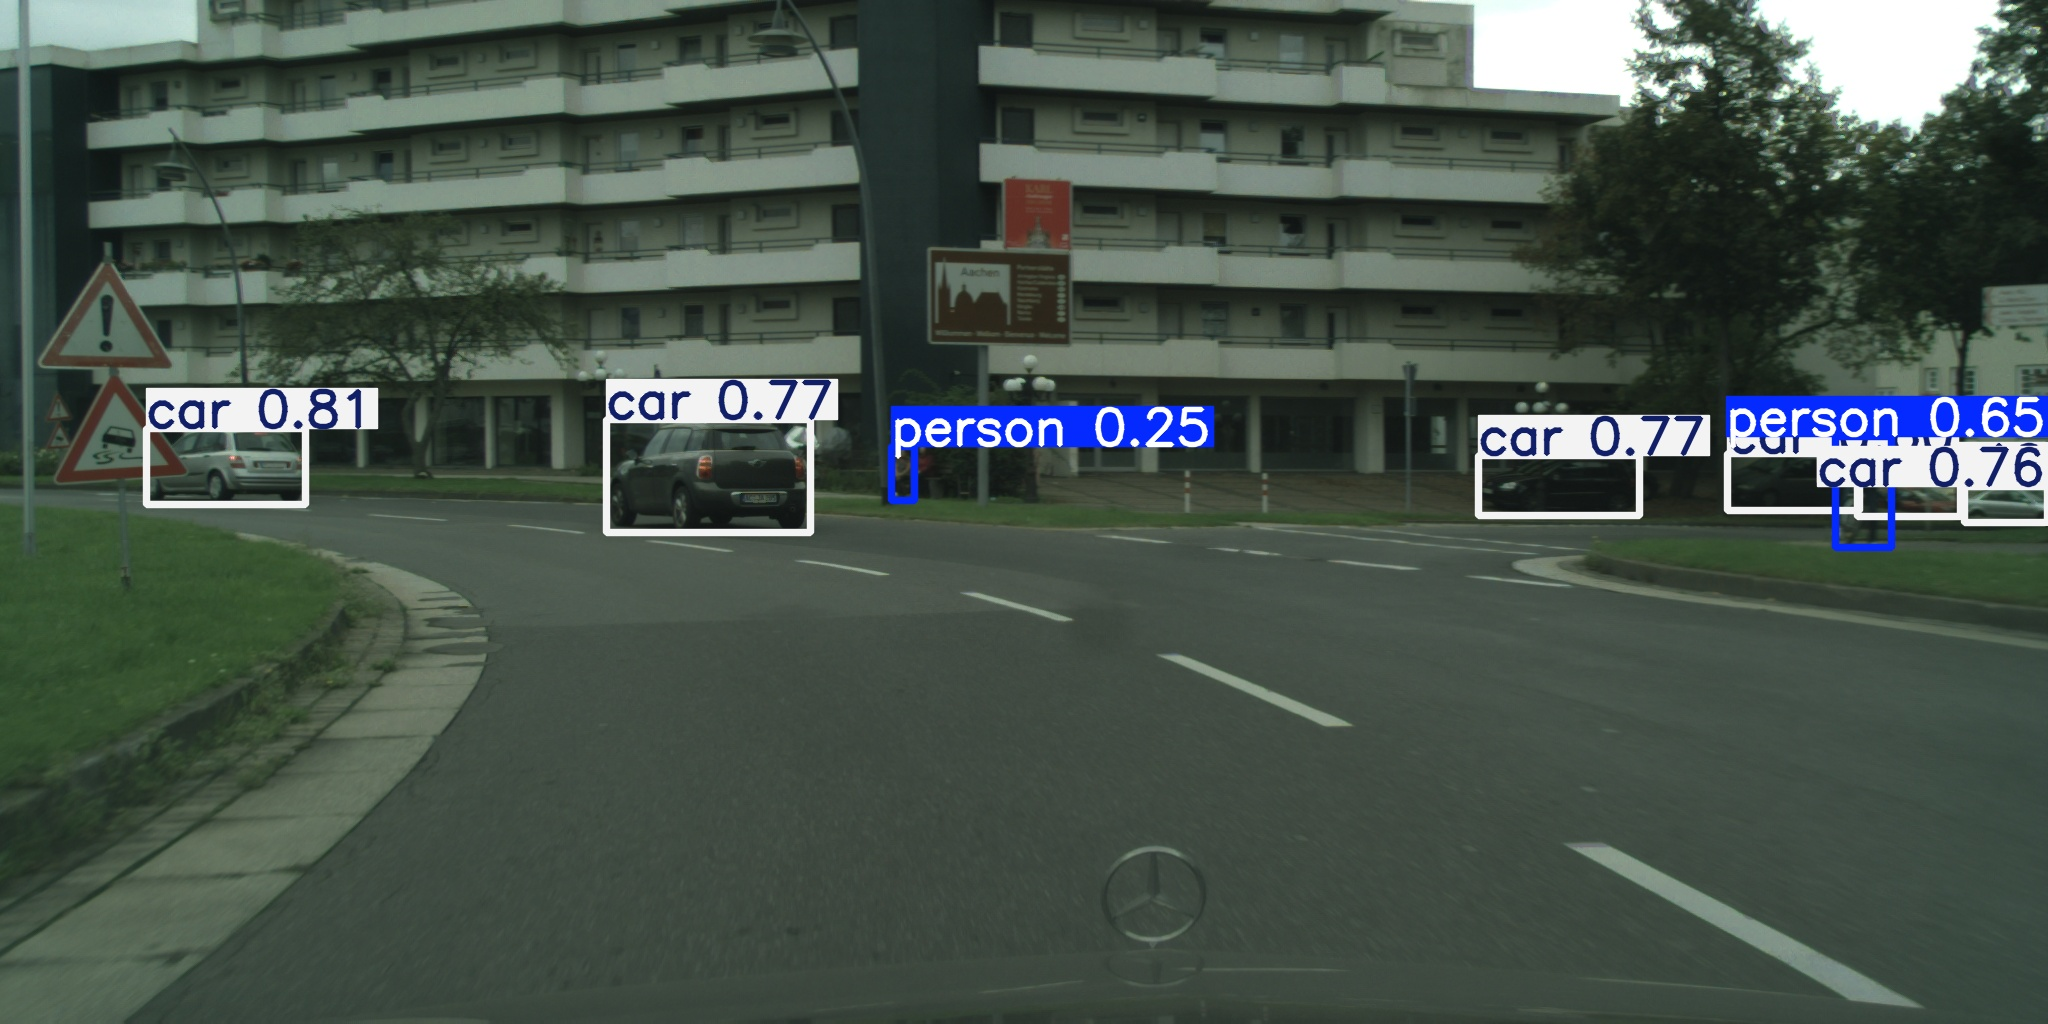
\includegraphics[scale=0.19]{pictures/original_aachen_000000.jpg}
            \caption{Erzeugtes Label aus dem Original Cityscapes Datensatz (Aachen erstes Bild) zur Objekterkennung durch das YOLO-Model.}
            \label{fig:og_aachen_000000}
        \end{figure}
        \begin{figure}[!htb]
            \centering
            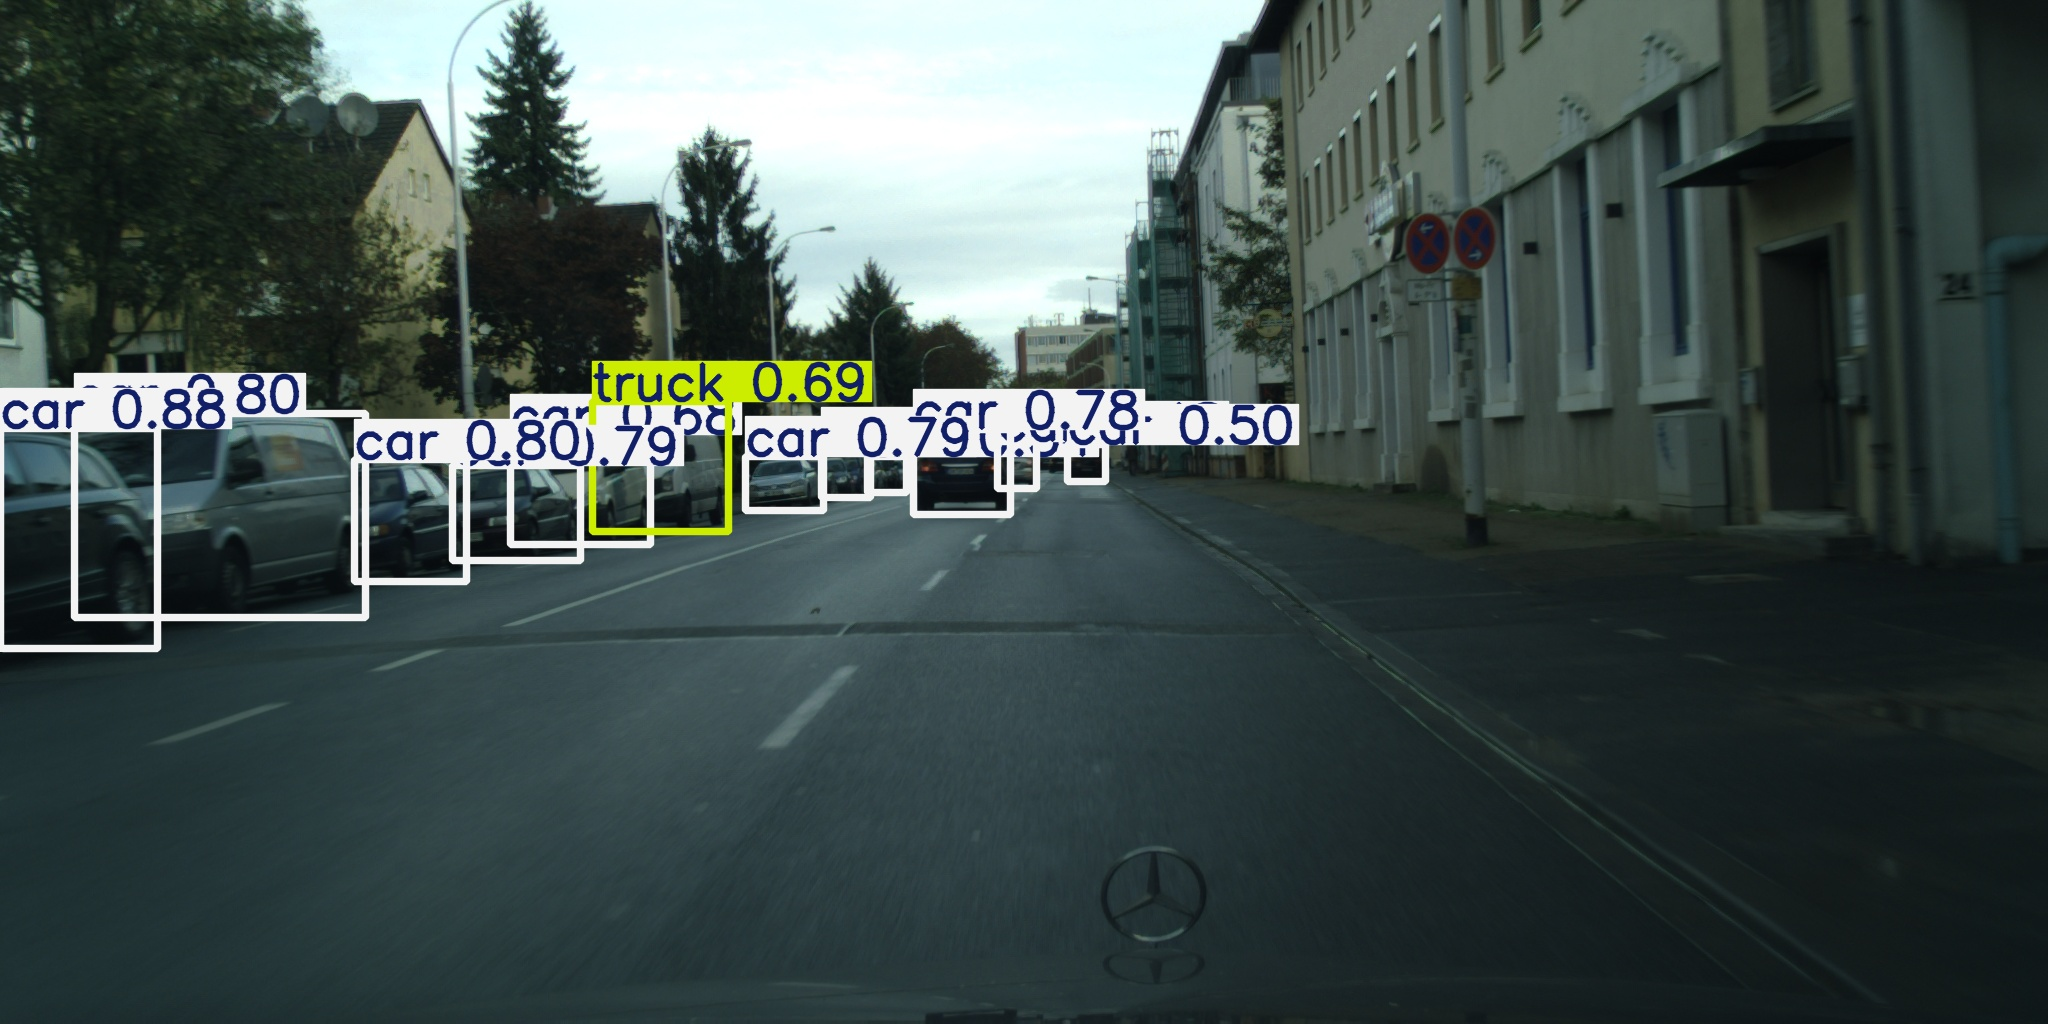
\includegraphics[scale=0.19]{pictures/original_darmstadt_000000.jpg}
            \caption{Erzeugtes Label aus dem Original Cityscapes Datensatz (Darmstadt drittes Bild) zur Objekterkennung durch das YOLO-Model.}
            \label{fig:og_darmstadt_000000}
        \end{figure}

\newpage  
        \subsection{JPEG-komprimierte Bilder}
            Für jedes Bild in den JPEG-Datensatz wurden Boundingboxen erstellt.
            \begin{figure}[!htb]
                \centering
                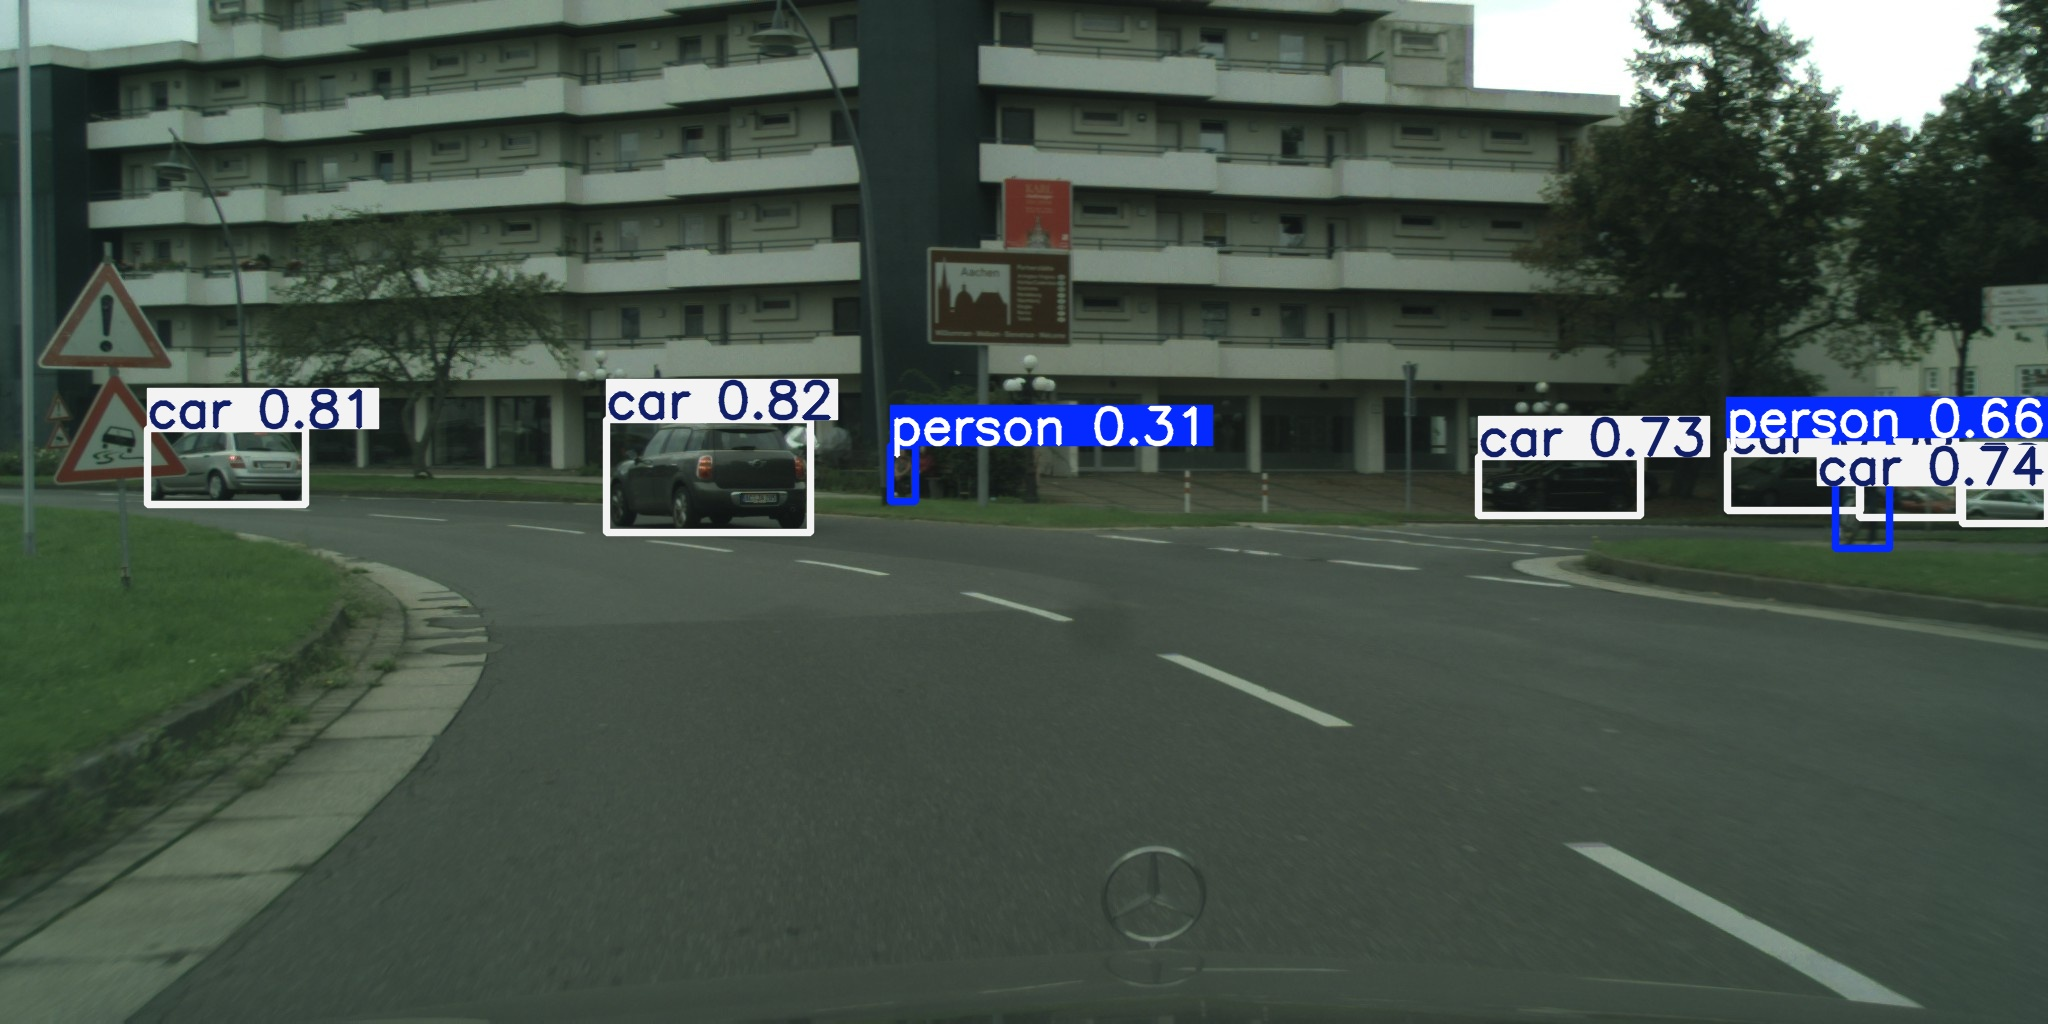
\includegraphics[scale=0.19]{pictures/jpg90_aachen_000000.jpg}
                \caption{Bild mit einer Kompressionsqualität von $90\%$ (Aachen, erstes Bild) zur Objekterkennung mit dem YOLO-Modell.}
                \label{fig:90_aachen_000000}
            \end{figure}
            \begin{figure}[!htb]
                \centering
                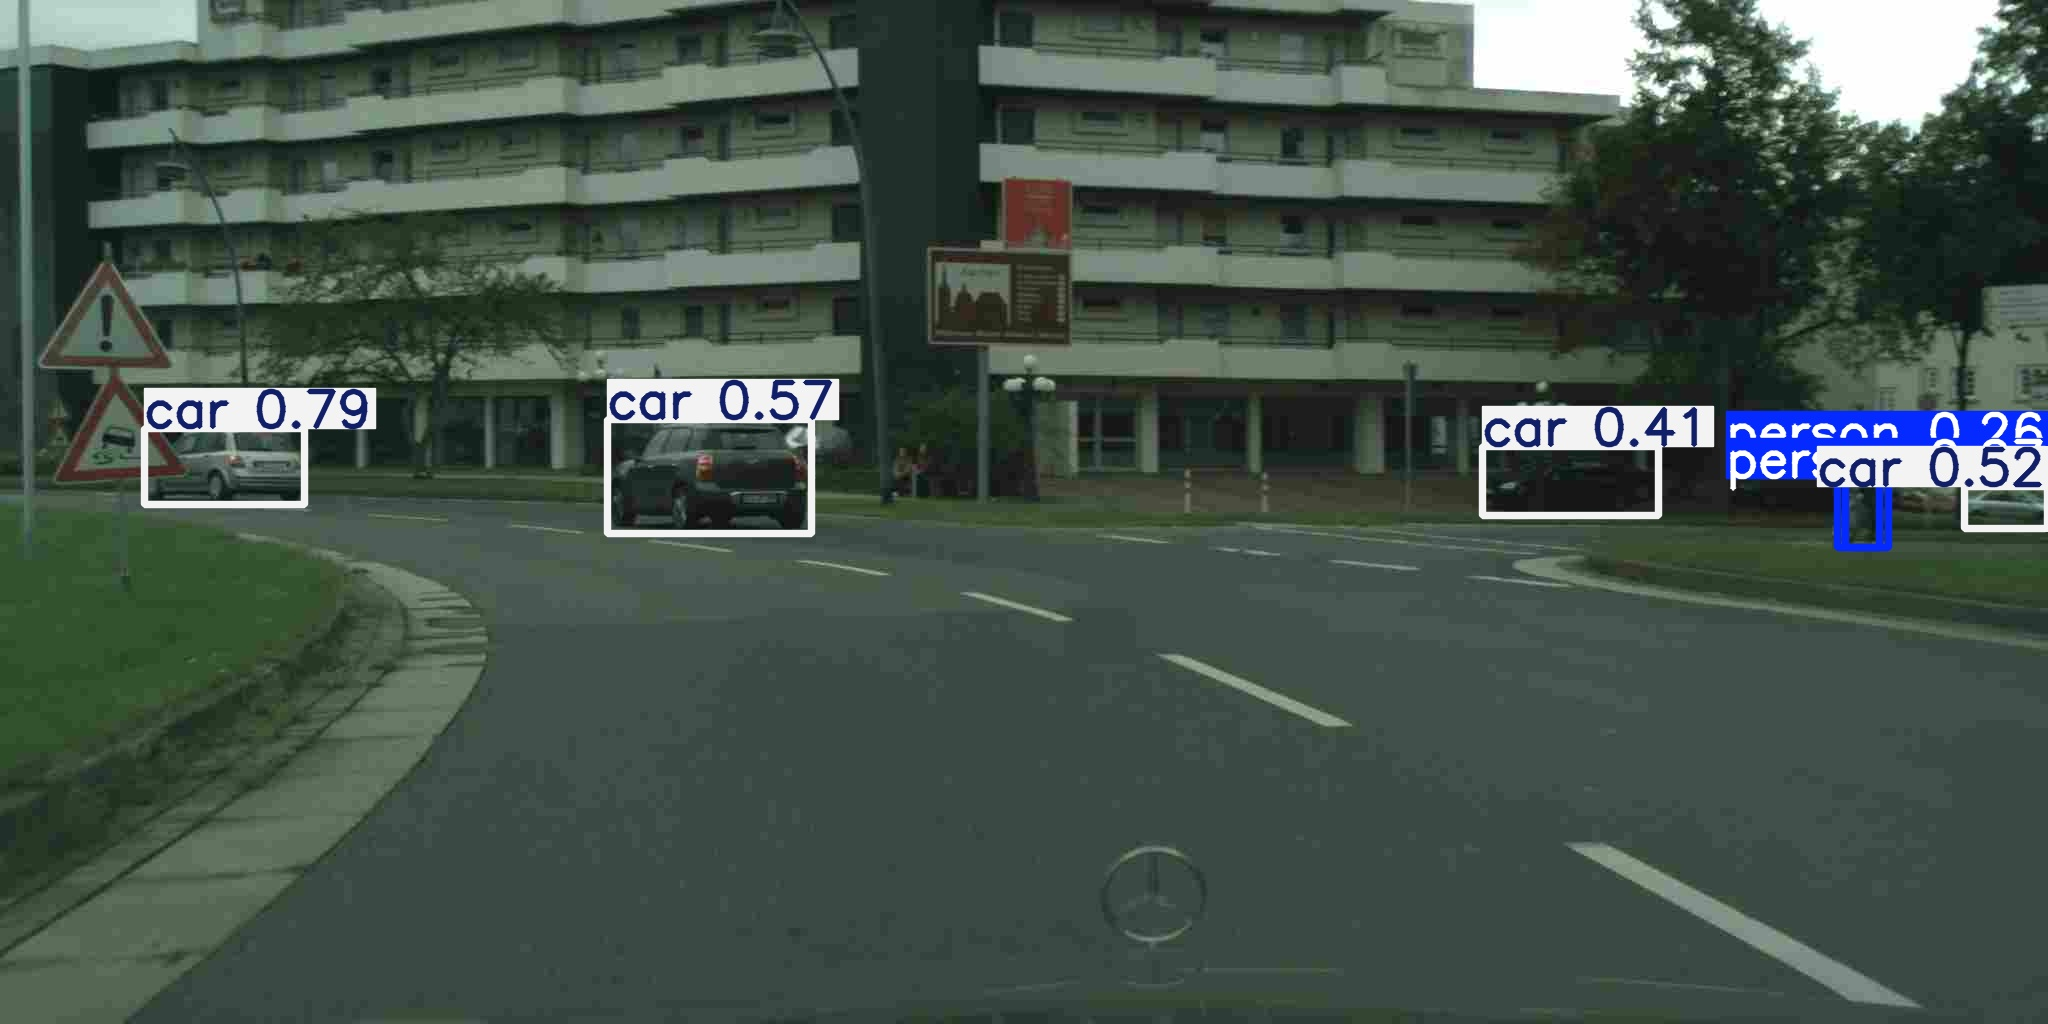
\includegraphics[scale=0.19]{pictures/jpg15_aachen_000000.jpg}
                \caption{Bild mit einer Kompressionsqualität von $15\%$ (Aachen, erstes Bild) zur Objekterkennung mit dem YOLO-Modell.}
                \label{fig:15_aachen_000000}
            \end{figure}
\newpage
            \begin{figure}[!htb]
                \centering
                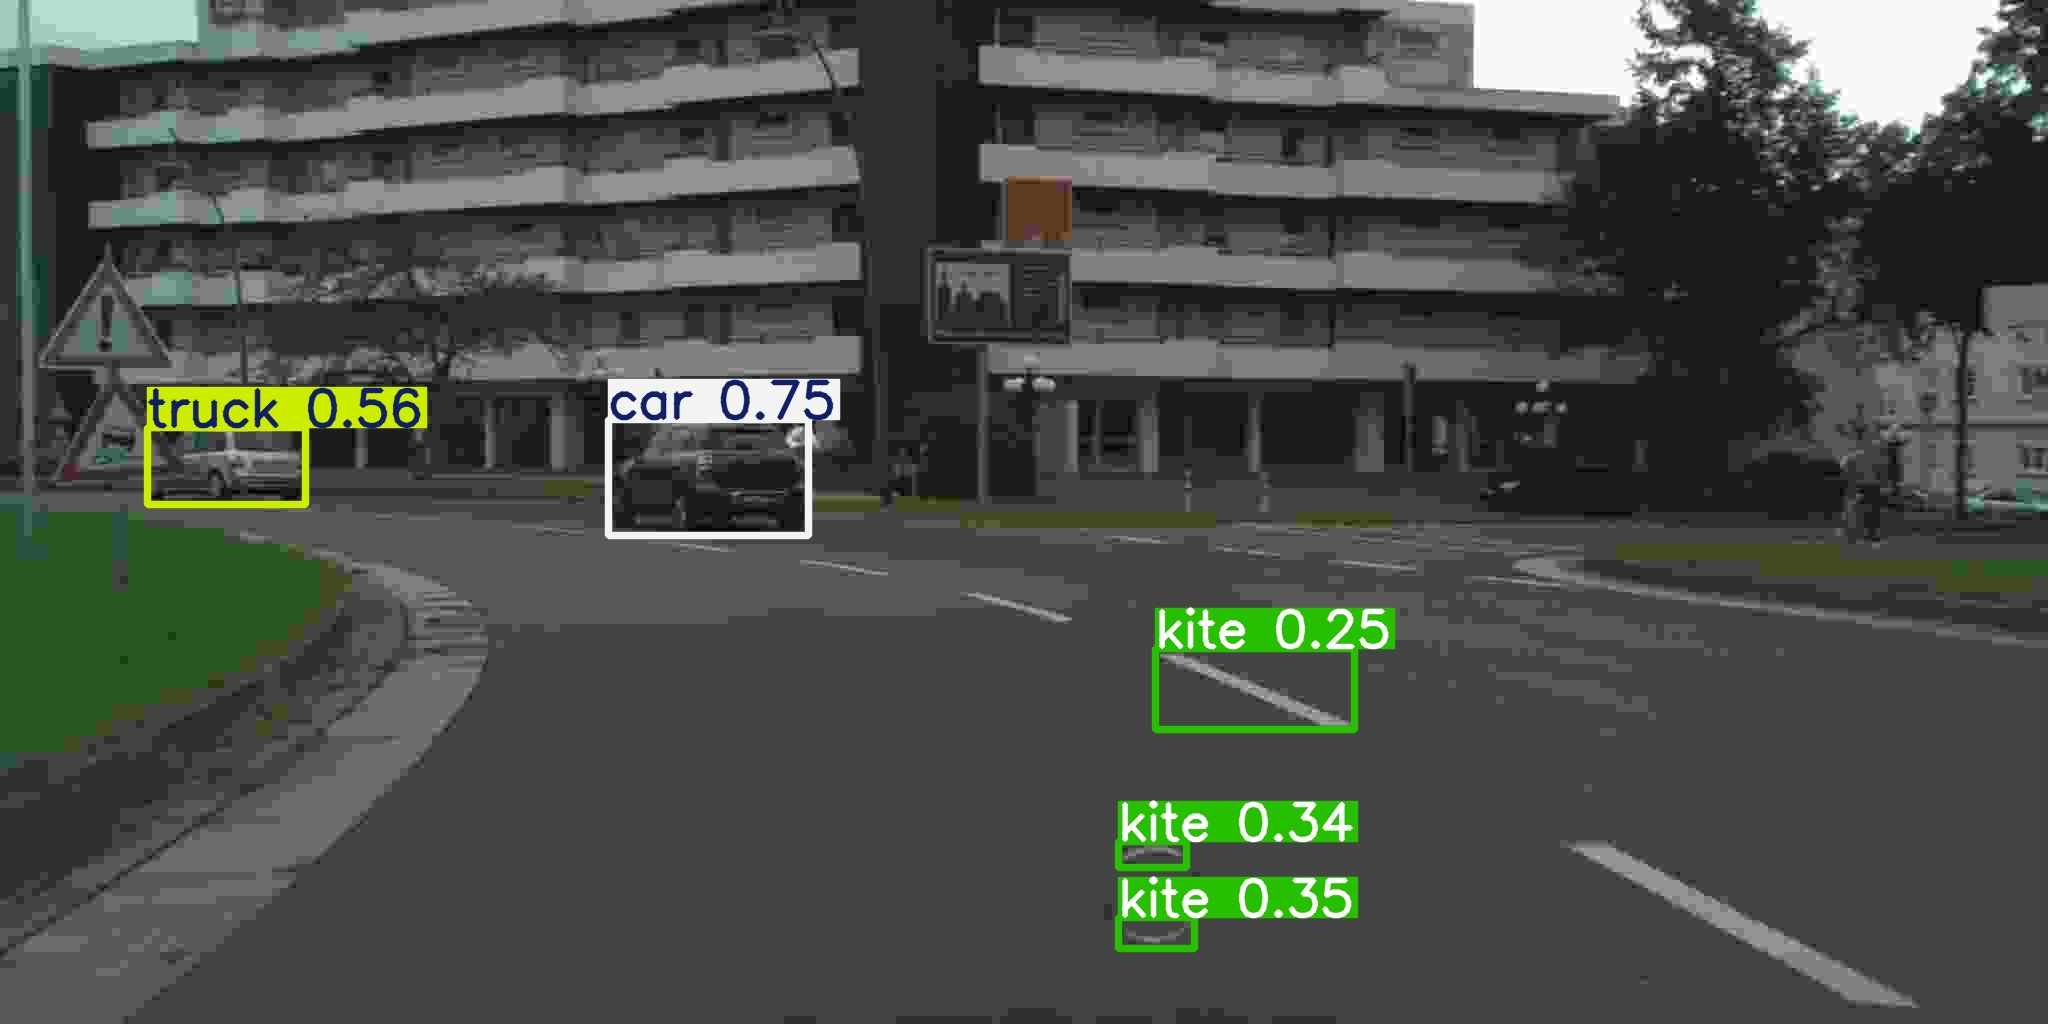
\includegraphics[scale=0.19]{pictures/jpg5_aachen_000000.jpg}
                \caption{Bild mit einer Kompressionsqualität von $5\%$ (Aachen, erstes Bild) zur Objekterkennung mit dem YOLO-Modell.}
                \label{fig:5_aachen_000000}
            \end{figure}

            Mit abnehmender Bildqualität werden Objekte undeutlicher, was das Erkennen von Objekten erheblich erschwert. Die prozentualen Wahrscheinlichkeiten der Klassifizierung sinken, wie in den Abbildungen \ref{fig:90_aachen_000000} und \ref{fig:15_aachen_000000} gut zu sehen ist. Dies führt dazu, dass Objekte entweder gar nicht erkannt oder falsch klassifiziert werden. Aufgrund der mangelnden Bildqualität werden teilweise sogar neue Objekte erkannt, wie in Abbildung \ref{fig:5_aachen_000000} „kite“.
            Dies lässt auf einen kausalen Zusammenhang schließen, dass Bilder mit schlechterer Qualität für eine Objektdetektion auch schlechter abschneiden. 
            Durch die abnehmende Bildqualität entstehen Fragmente sowie farblich falsche Kontraste, Helligkeits- und Sättigungswerte, wie deutlich in Abbildung \ref{fig:5_aachen_000000} zu sehen ist. Das Auto, welches in jedem der drei Bilder erkannt wird, weist verschiedene Wahrscheinlichkeiten auf, zur Klasse „Car“ zu gehören – und dies nicht in einer klar absteigenden Reihenfolge in Abhängigkeit von der Bildqualität.
            Im Originalbild (Abbildung \ref{fig:og_aachen_000000}) liegt die Wahrscheinlichkeit bei $77\%$. Bei dem Bild mit einer Kompressionsqualität von $90\%$ (Abbildung \ref{fig:90_aachen_000000}) steigt die Wahrscheinlichkeit auf $82\%$. In Abbildung \ref{fig:15_aachen_000000} sinkt die Wahrscheinlichkeit, wie man es bei einem Bild mit schlechterer Qualität erwarten würde, auf $57\%$. Erstaunlicherweise erreicht das Bild mit lediglich $5\%$ Kompressionsqualität (Abbildung \ref{fig:5_aachen_000000}) fast die gleiche Wahrscheinlichkeit wie das Originalbild, nämlich $75\%$.
            Dies zeigt, dass auch das Modell eine Rolle spielt, das die Objekte erkennen soll und hat ebenso wie die Qualität des Bildes einen Einfluss darauf, wie gut Objekte erkannt werden. Dies gilt trotz der Tatsache, dass die Labels und die komprimierten Datensätze alle mit demselben Modell erstellt wurden.\\
            \textbf{Kompressionsqualität $5\%$}:\\
            $\text{true positives} = 1 \quad \text{false positives} = 4 \quad \text{false negatives} = 7$
            
\newpage   
            \begin{figure}[!htb]
                \centering
                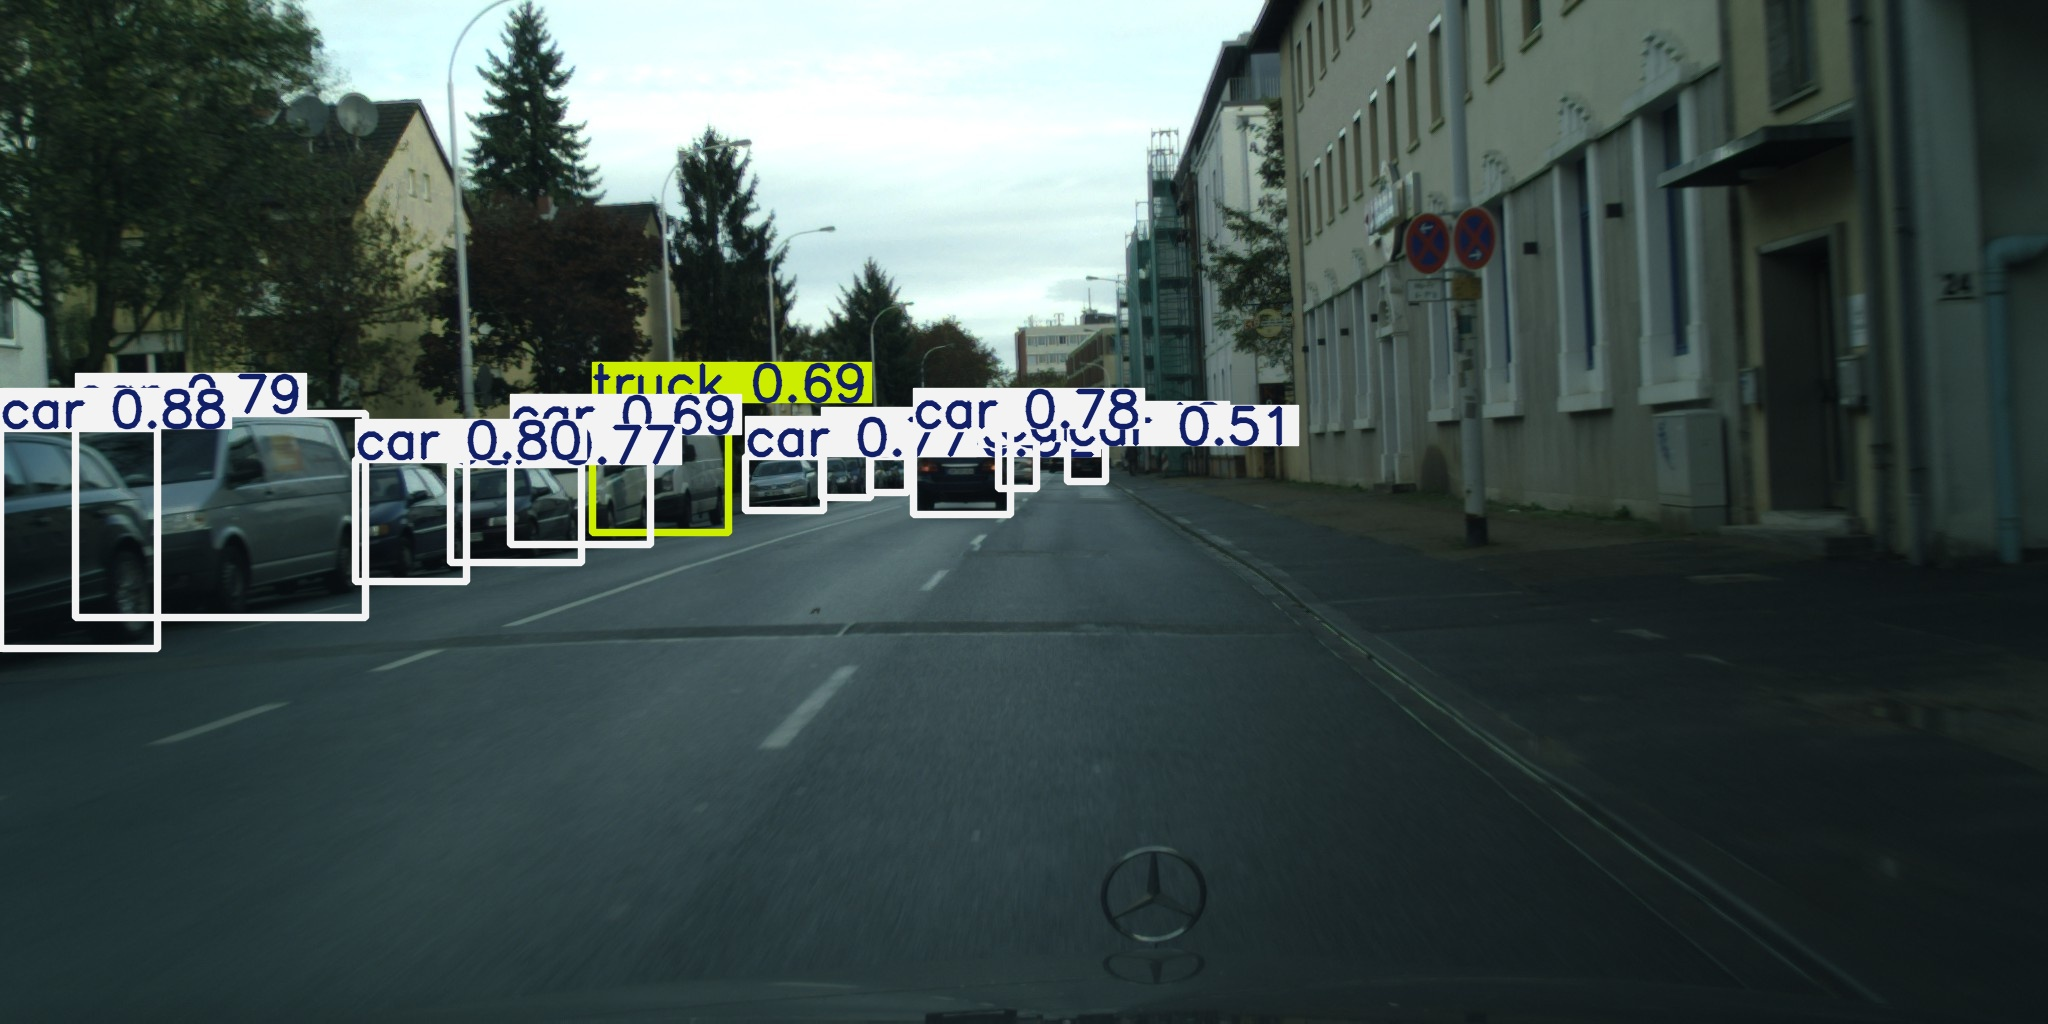
\includegraphics[scale=0.19]{pictures/jpg90_darmstadt_000000.jpg}
                \caption{Bild aus dem Cityscapes-Datensatz mit einer JPEG-Kompressionsqualität von $90\%$ (Darmstadt, erstes Bild), verarbeitet zur Objekterkennung durch das YOLO-Modell.}
                \label{fig:90_darmstadt_000000}
            \end{figure}
            \begin{figure}[!htb]
                \centering
                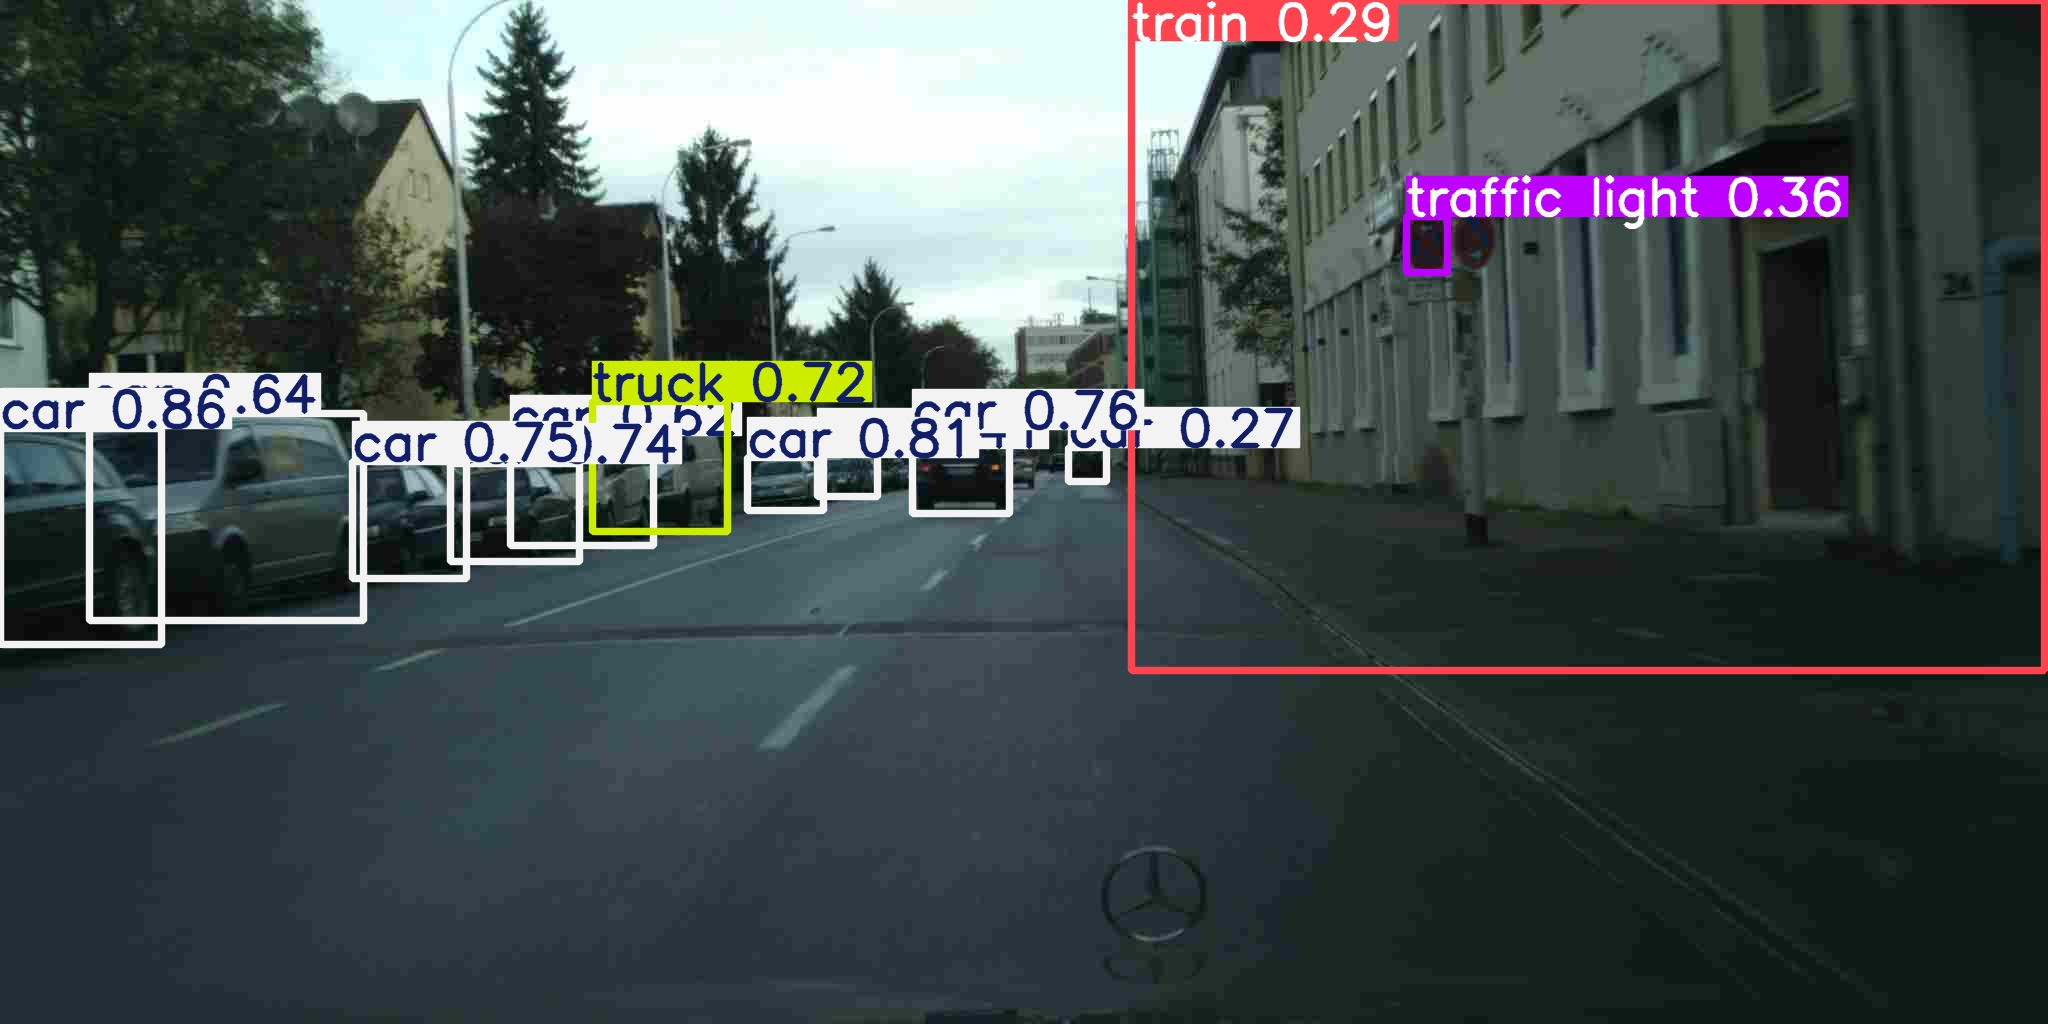
\includegraphics[scale=0.19]{pictures/jpg15_darmstadt_000000.jpg}
                \caption{Bild aus dem Cityscapes-Datensatz mit einer JPEG-Kompressionsqualität von $15\%$ (Darmstadt, erstes Bild), verarbeitet zur Objekterkennung durch das YOLO-Modell.}
                \label{fig:15_darmstadt_000000}
            \end{figure}

\newpage    
            \begin{figure}[!htb]
                \centering
                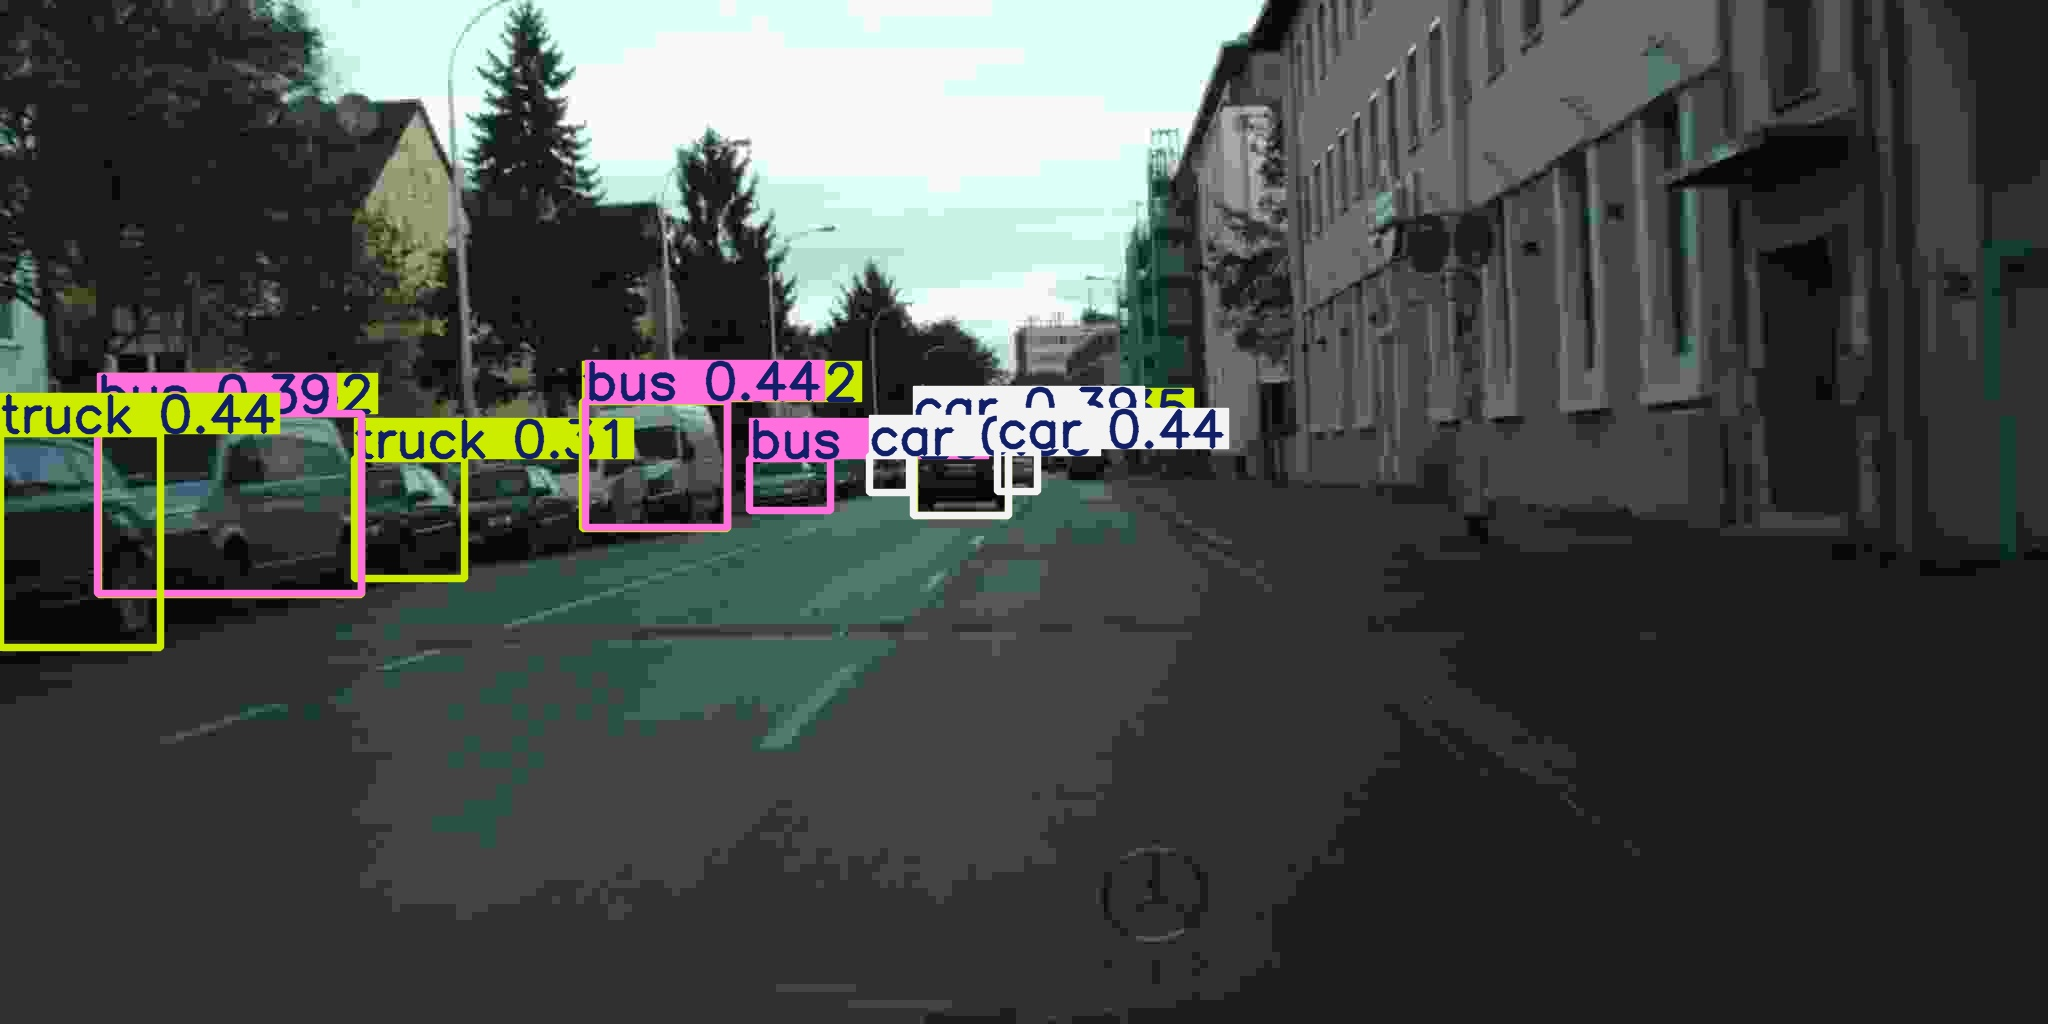
\includegraphics[scale=0.19]{pictures/jpg5_darmstadt_000000.jpg}
                \caption{Bild aus dem Cityscapes-Datensatz mit einer JPEG-Kompressionsqualität von $5\%$ (Darmstadt, erstes Bild), verarbeitet zur Objekterkennung durch das YOLO-Modell.}
                \label{fig:5_darmstadt_000000}
            \end{figure}

            Auch auf den Darmstadt-Bildern in den Abbildungen \ref{fig:90_darmstadt_000000}, \ref{fig:15_darmstadt_000000} und \ref{fig:5_darmstadt_000000} ist deutlich zu erkennen, wie die Objektdetektion bei abnehmender Qualität darunter leidet. So wurde beispielsweise in Abbildung \ref{fig:15_darmstadt_000000} eine ganze Häuserfassade fälschlicherweise als Zug klassifiziert. Auffällig ist außerdem, dass gewöhnliche Autos bei geringerer Qualität häufig als „truck“ oder „bus“ falsch klassifiziert werden.
            Diese Fehlklassifizierung der Autos tritt bei jedem Bild auf, sobald die Kompressionsqualität zu
            gering wird und die Artefakte im Bild deutlich zu erkennen sind.
            Dies liegt jedoch am YOLO-Modell. „truck“, „bus“ und „car“ müssen ähnliche Merkmalsrepräsentationen aufweisen.
            YOLO11 ist ein CNN und verwendet Feature Maps, die Muster aus Bildern extrahieren. Wenn „truck“, „bus“ und „car“ ähnliche Werte aufweisen, bedeutet das, dass ihre Merkmale (z.B. Kanten, Konturen, Formen) sich stark überschneiden.
            

\newpage  
            \underline{\textbf{Metriken zum Vergleich von Bildern mit Labels}}        
            \begin{figure}[!htb]
                \centering
                \includesvg[scale=0.56]{graphs/output_plot_f1_pr_re.svg}
                \caption{Diese Grafik zeigt die Metriken Precison, Recall und F1 Score in Abhängigkeit zur Kompressionsqualität.}
                \label{fig:pr_f1_re}
            \end{figure}

            Der F1-Score sowie Precision und Recall sind gängige Metriken zur Überprüfung,
            wie gut ein Modell einen Datensatz auf die dazugehörigen Labels abbildet und klassifiziert.
            Es ist zu erkennen, dass bei einer Kompressionsqualität von $85\%$–$100\%$ die drei Metriken nahe bei 1,0 liegen (1,0 entspräche den Originaldaten). Precision verläuft dabei sehr flach – flacher als Recall und der F1-Score. Mit einer nahezu null Steigung bleibt sie bis zu einer Kompressionsqualität von etwa $25\%$–$30\%$ konstant. Erst unterhalb dieser Werte beginnt die Kurve erkennbar abzufallen.
            Dies haben alle drei Metriken gemeinsam: Sie fallen ab, sobald die Kompressionsqualität unterhalb dieser Werte sinkt. Die Kurven spiegeln das wider, was man in den Bildern mit verschiedenen Kompressionsqualitäten bereits sehen konnte.   
            Die Differenz der $y$-Werte (Metriken-Scores) bei gleicher $x$-Werte (Kompressionsqualität) nimmt zu, je geringer die Kompressionsqualität wird. Die drei Kurven starten bei $100\%$ nahezu am selben Punkt und driften vom F1-Wert zunehmend ab.
            Bis zu Werten von $75\%$ weichen Precision und Recall maximal um $y = \pm 0,02$ vom F1-Score ab. Über einen Bereich von $x = 50$ Einheiten hinweg steigen die Abweichungen maximal auf $y = \pm 0,03$. Erst unterhalb von $30\%$ driften die Kurven stark auseinander. Bei $x = 5$ erreichen Precision $y = +0,2$ und $y = -0,1$ für Recall, abweichend vom F1-Score.
            
\newpage            
            \begin{figure}[!htb]
                \centering
                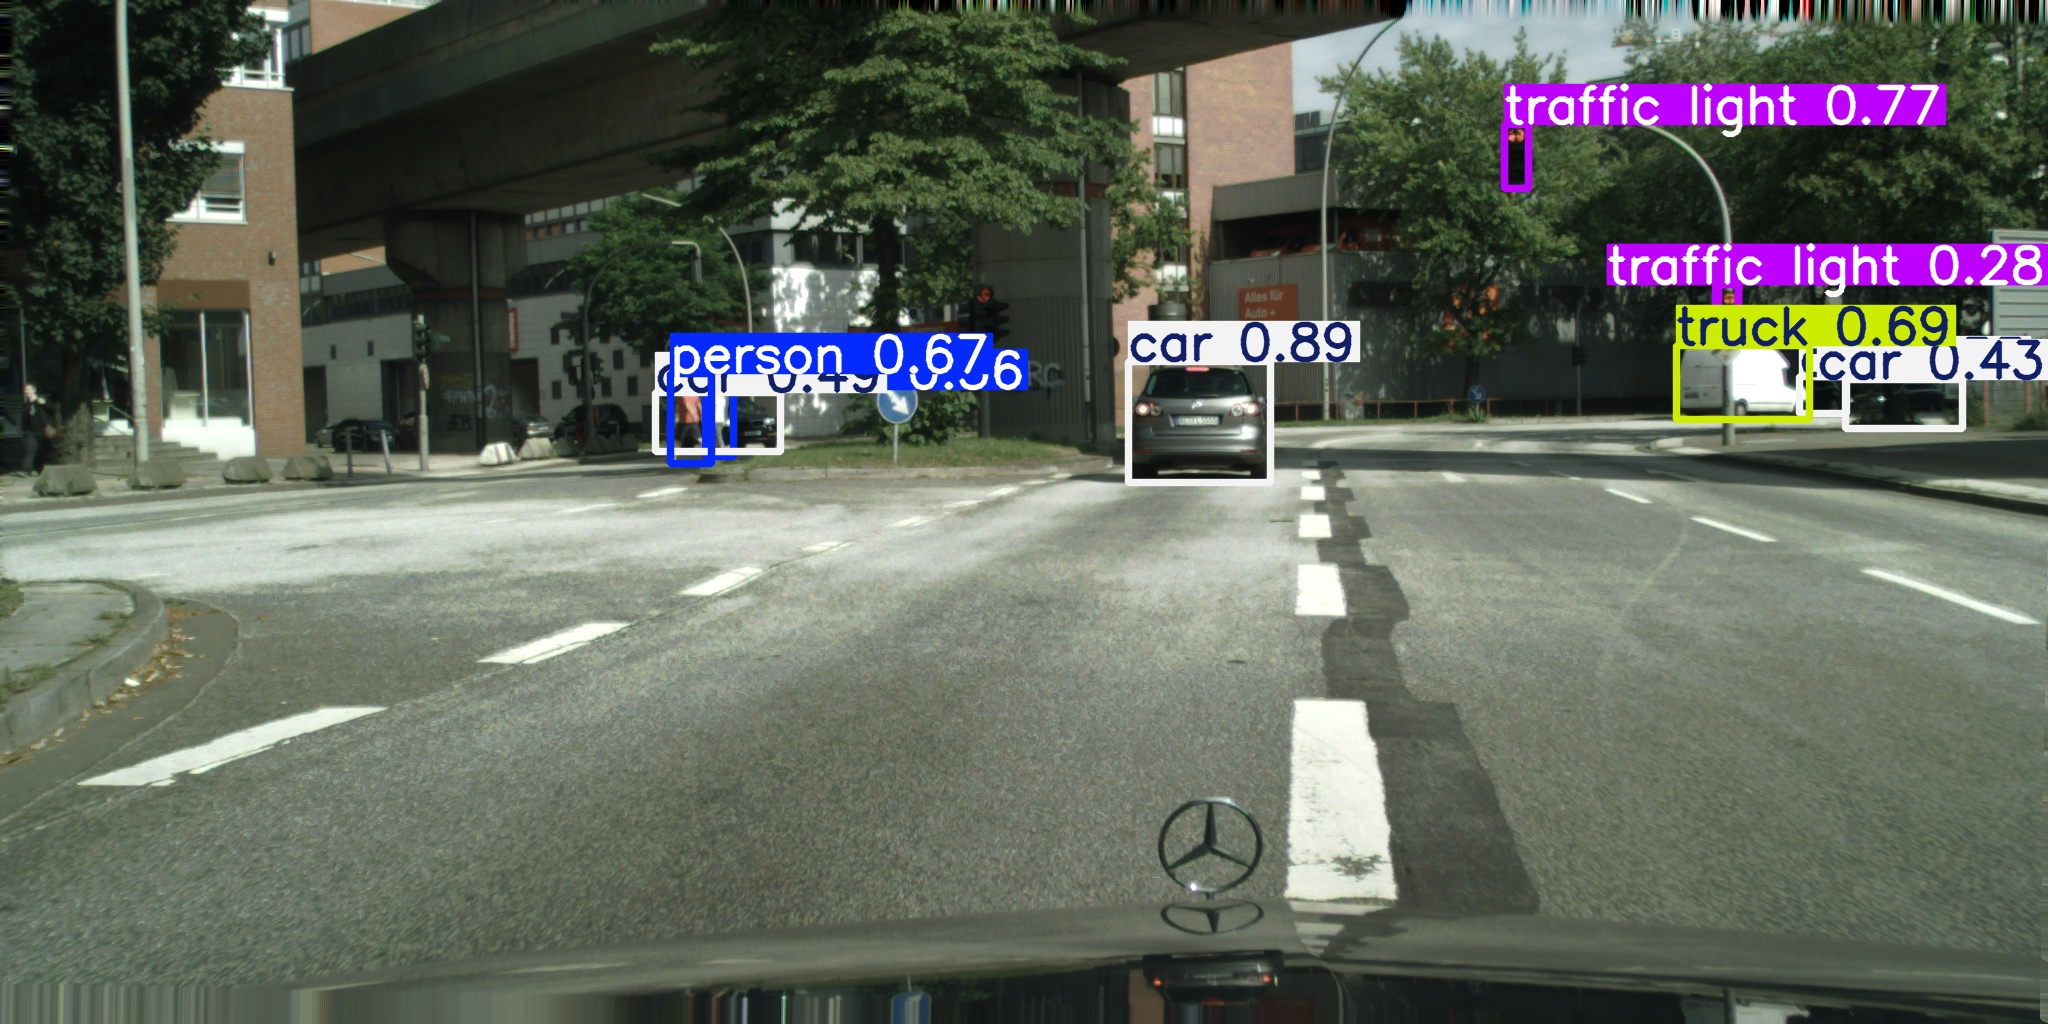
\includegraphics[scale=0.19]{pictures/original_hamburg_000000.jpg}
                \caption{Original Label Bild aus dem Cityscapes Datensatz (Hamburg sechstes Bild) zur Objekterkennung durch das YOLO- Model.}
                \label{fig:og_hamburg_6}
            \end{figure}
            \begin{figure}[!htb]
                \centering
                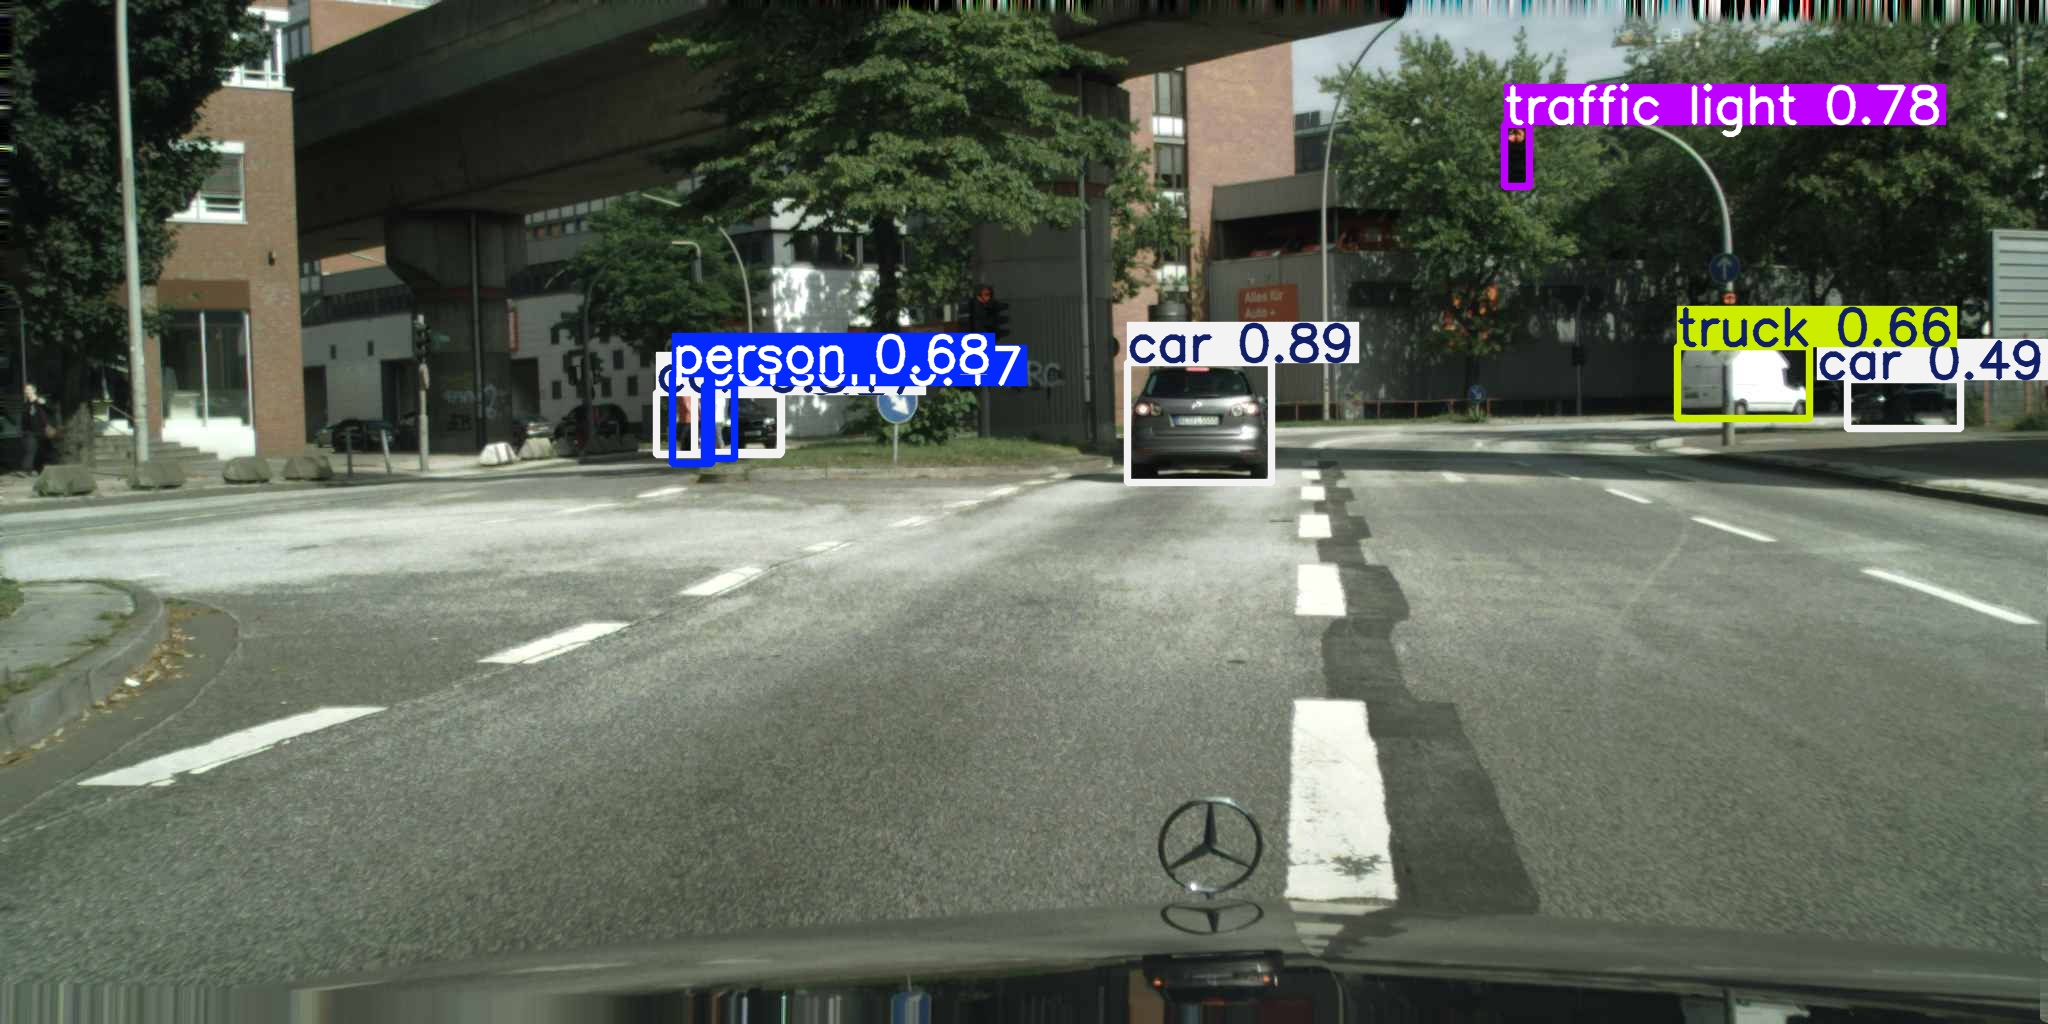
\includegraphics[scale=0.19]{pictures/jpg40_hamburg_000000.jpg}
                \caption{Bild aus dem Cityscapes-Datensatz mit einer JPEG-Kompressionsqualität von $40\%$ (Hamburg, sechstes Bild), verarbeitet zur Objekterkennung durch das YOLO-Modell.}
                \label{fig:jpg40_hamburg_6}
            \end{figure}
\newpage
            
            \begin{figure}[!htb]
                \centering
                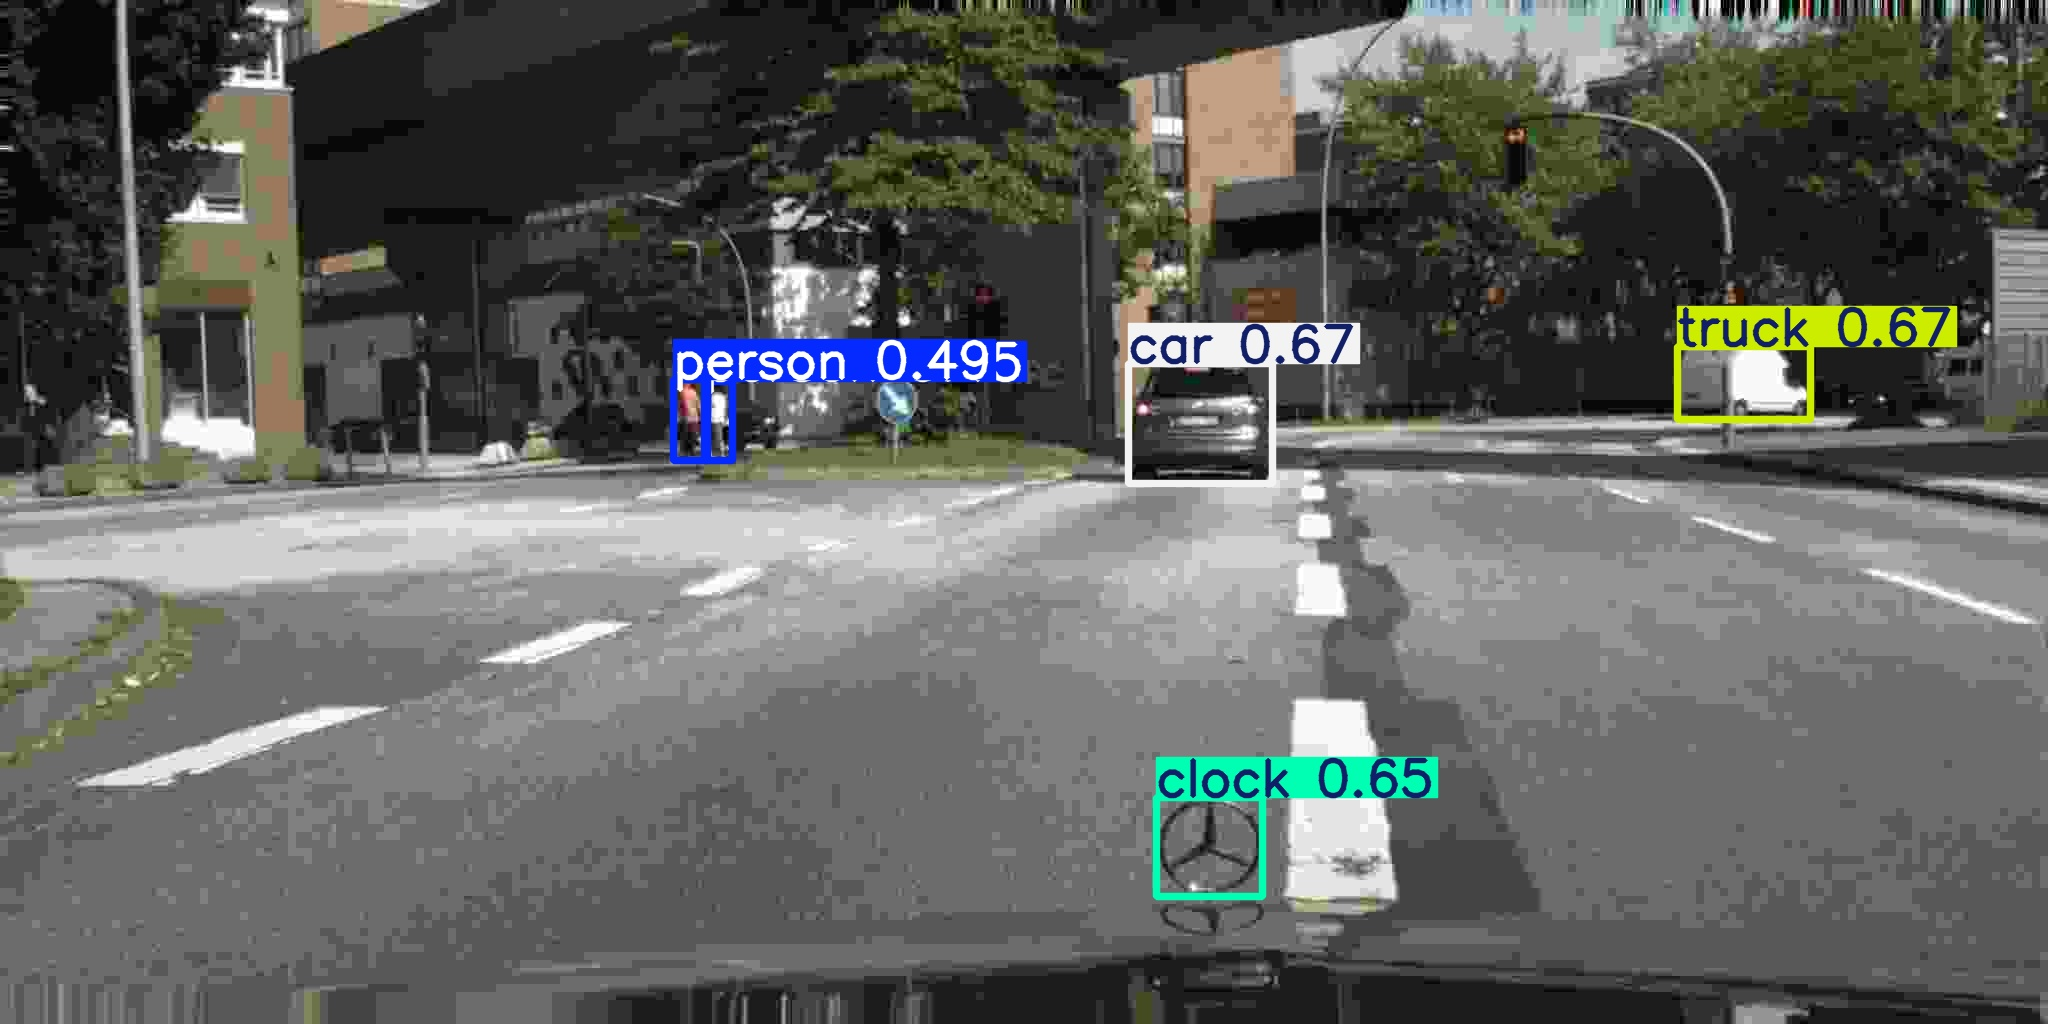
\includegraphics[scale=0.19]{pictures/jpg5_hamburg_000000.jpg}
                \caption{Bild aus dem Cityscapes-Datensatz mit einer JPEG-Kompressionsqualität von $5\%$ (Hamburg, sechstes Bild), verarbeitet zur Objekterkennung durch das YOLO-Modell.}
                \label{fig:jpg5_hamburg_6}
            \end{figure}

            Bei den Bildern aus Hamburg sieht man, dass die Grafik \ref{fig:pr_f1_re} die Ergebnisse korrekt darstellt, da kaum ein Unterschied in der Objektdetektion zwischen \ref{fig:jpg40_hamburg_6} und \ref{fig:og_hamburg_6} erkennbar ist – abgesehen von einem fehlenden „traffic light“. Auffällig ist zudem, dass in Abbildung \ref{fig:jpg5_hamburg_6} bei einer Kompressionsqualität von $5\%$ die Klassifizierung des „Truck“ mit einem Wert von $67\%$ angegeben wird, was $1\%$ höher ist als bei einer Kompressionsqualität von $40\%$ in Abbildung \ref{fig:jpg40_hamburg_6}.
            Dies lässt erneut darauf schließen, dass nicht nur der Grad der Komprimierung, sondern auch das Modell zur Objektdetektion selbst eine Rolle dabei spielt, wie gut ein Objekt auf qualitativ schlechteren Bildern erkannt wird.
            Auch ist hier zu sehen, dass der Mercedes-Stern als „clock“ klassifiziert wird. Da alle Datensätze auch die Labels mit demselben Modell für die Boundingboxen erstellt wurden, wäre zu erwarten gewesen, dass ein Bild besserer Qualität, wie das Label, an dieser Stelle ebenfalls als „clock“ klassifiziert worden wäre, was jedoch nicht der Fall ist. 
            Dies zeigt, dass durch mangelnde Bildqualität Fehlklassifizierungen entstehen.
            
\newpage  
            \underline{\textbf{Intersection over Union (IoU)}}\bigskip
            
            Um die Qualität der Bounding-Boxen zu überprüfen und zu bewerten, inwieweit sie mit den Ground-Truth-Boundingboxen übereinstimmen, wird der IoU verwendet.
            
            \begin{figure}[!htb]
                \centering
                \includesvg[scale=0.56]{graphs/output_plot_iou.svg}
                \caption{IoU in Abhängigkeit zur Kompressionsqualität.}
                \label{fig:iou}
            \end{figure}
            Auch der IoU liegt anfangs von $100\%$ bis zu einer Kompressionsqualität von $25\%$ in guten Wertebereichen oberhalb von $0,8$ teils $0,9$. Unterhalb von $25\%$ fällt der IoU ab auf $0,5$ bei $5\%$ Kompressionsqualität. Der IoU weist innerhalb von $20$ Einheiten auf der $x$-Achse von $5\%$ bis $25\%$ eine Differenz von $0,35$ auf. Von $25\%$ bis $100\%$ über $75$ Einheiten hinweg ist lediglich eine Differenz von $0,17$ Einheiten vorhanden. Dies zeigt erneut den Qualitätsunterschied von Bildern oberhalb der JPEG-Kompressionsqualität von $25\%$ bis $30\%$ und derer, die darunter liegen. Diese Gemeinsamkeit weisen alle Metriken auf, welche in dieser Arbeit betrachtet werden, dass unterhalb dieser Schwellwerte sich die Werte deutlich verschlechtern.
            Bei näherer Betrachtung zeigt der IoU nahezu identische Kurvenverläufe wie der Recall in Abbildung \ref{fig:pr_f1_re}. Ein Unterschied der beiden Kurven besteht darin, dass der IoU von ($x = 25$, $y = 0,79$) über die nächsten $75$ Einheiten bis zu ($x = 100$, $y = 0,961$) etwas steiler ansteigt. Recall liegt bei ($x = 25$, $y = 0,864$) mit $0,075$ Einheiten über dem IoU und bei ($x = 100$, $y = 0,975$) um $0,014$ Einheit darüber. Auch hier ist bei $50\%$ ein Wendepunkt in der Kurve.
            

\newpage
            \begin{figure}[!htb]
                \centering
                \includesvg[scale=0.56]{graphs/output_plot_iou_std.svg}
                \caption{Diese Grafik zeigt den IoU in Abhängigkeit zur Kompressionsqualität mit Standartabweichung.}
                \label{fig:iou_std}
            \end{figure}
            
            Die Standardabweichung liegt mit $100\%$ Kompressionsqualität noch bei $0,13$, erhöht sich jedoch bis auf $0,44$ bei einer Kompressionsqualität von $5\%$. Die Standardabweichung wird auf den Mittelwert addiert  bzw. subtrahiert. Aufgrund der stark variierenden Werte kann die Summe aus Mittelwert und Standardabweichung auch über $1,0$ liegen, obwohl die einzelnen IoU-Werte immer zwischen $0$ und $1$ liegen. Die einzelnen IoU-Werte reichen von $0,99$ bis hin zu $0,0$.
            Dies liegt daran, dass die Berechnung des IoU einen Schwellenwert (Threshold) hat. Bei Werten unter $0,5$ wird der IoU auf Null gesetzt. Dadurch ergeben sich zahlreiche Werte, die entweder bei Null oder nahe $1,0$ liegen können.\\
\newpage
            \begin{table}[h!]
                \centering
                \begin{tabular}{rl}
                    \toprule
                    \textbf{Index} & \textbf{Wert (gerundet)} \\
                    \midrule
                    1  & 0.9816 \\
                    2  & 0.0 \\
                    3  & 0.9579 \\
                    4  & 0.0 \\
                    5  & 0.0 \\
                    6  & 0.0 \\
                    7  & 0.0 \\
                    8  & 0.0 \\
                    9  & 0.9438 \\
                    10 & 0.9256 \\
                    11 & 0.8562 \\
                    12 & 0.9276 \\
                    13 & 0.7814 \\
                    14 & 0.8782 \\
                    15 & 0.9729 \\
                    16 & 0.0 \\
                    17 & 0.5183 \\
                    18 & 0.8200 \\
                    19 & 0.0 \\
                    20 & 0.9788 \\
                    \bottomrule
                \end{tabular}
                \caption{Die ersten Gerundeten 20 IoU-Werte für eine Kompressionsqualität von $5\%$ (4 Nachkommastellen)}
                \label{tab:compression5}
            \end{table}

            Die ersten 20 IoU-Werte des Datensatzes mit einer Kompressionsqualität von $5\%$ zeigen deutlich, dass die Werte oft weit auseinanderliegen. Dies ist auf den Schwellenwert (Threshold) bei der Berechnung des IoU zurückzuführen: Nur Werte mit $IoU > 0,5$ werden berücksichtigt, während alle darunterliegenden Werte auf $0,0$ gesetzt werden.\\

            \begin{center}
                \underline{Hinweis:}\\
                In die Berechnung des IoU wurden alle Werte einbezogen, die oberhalb des Schwellenwerts (Threshold) liegen, sowie alle Null-Werte (Werte unterhalb des Schwellenwerts), um die tatsächliche Performance des Modells und der Bilder zu untersuchen. Boundingboxen ohne zugehörige Ground-Truth-Boundingbox-Labels und umgekehrt wurden jedoch \textbf{nicht} berücksichtigt und auch \textbf{nicht} als Null-Werte in die Berechnung einbezogen.
            \end{center}
            
\newpage
        \subsection{KI-rekonstruierte Bilder}
            \begin{figure}[!htb]
                \centering
                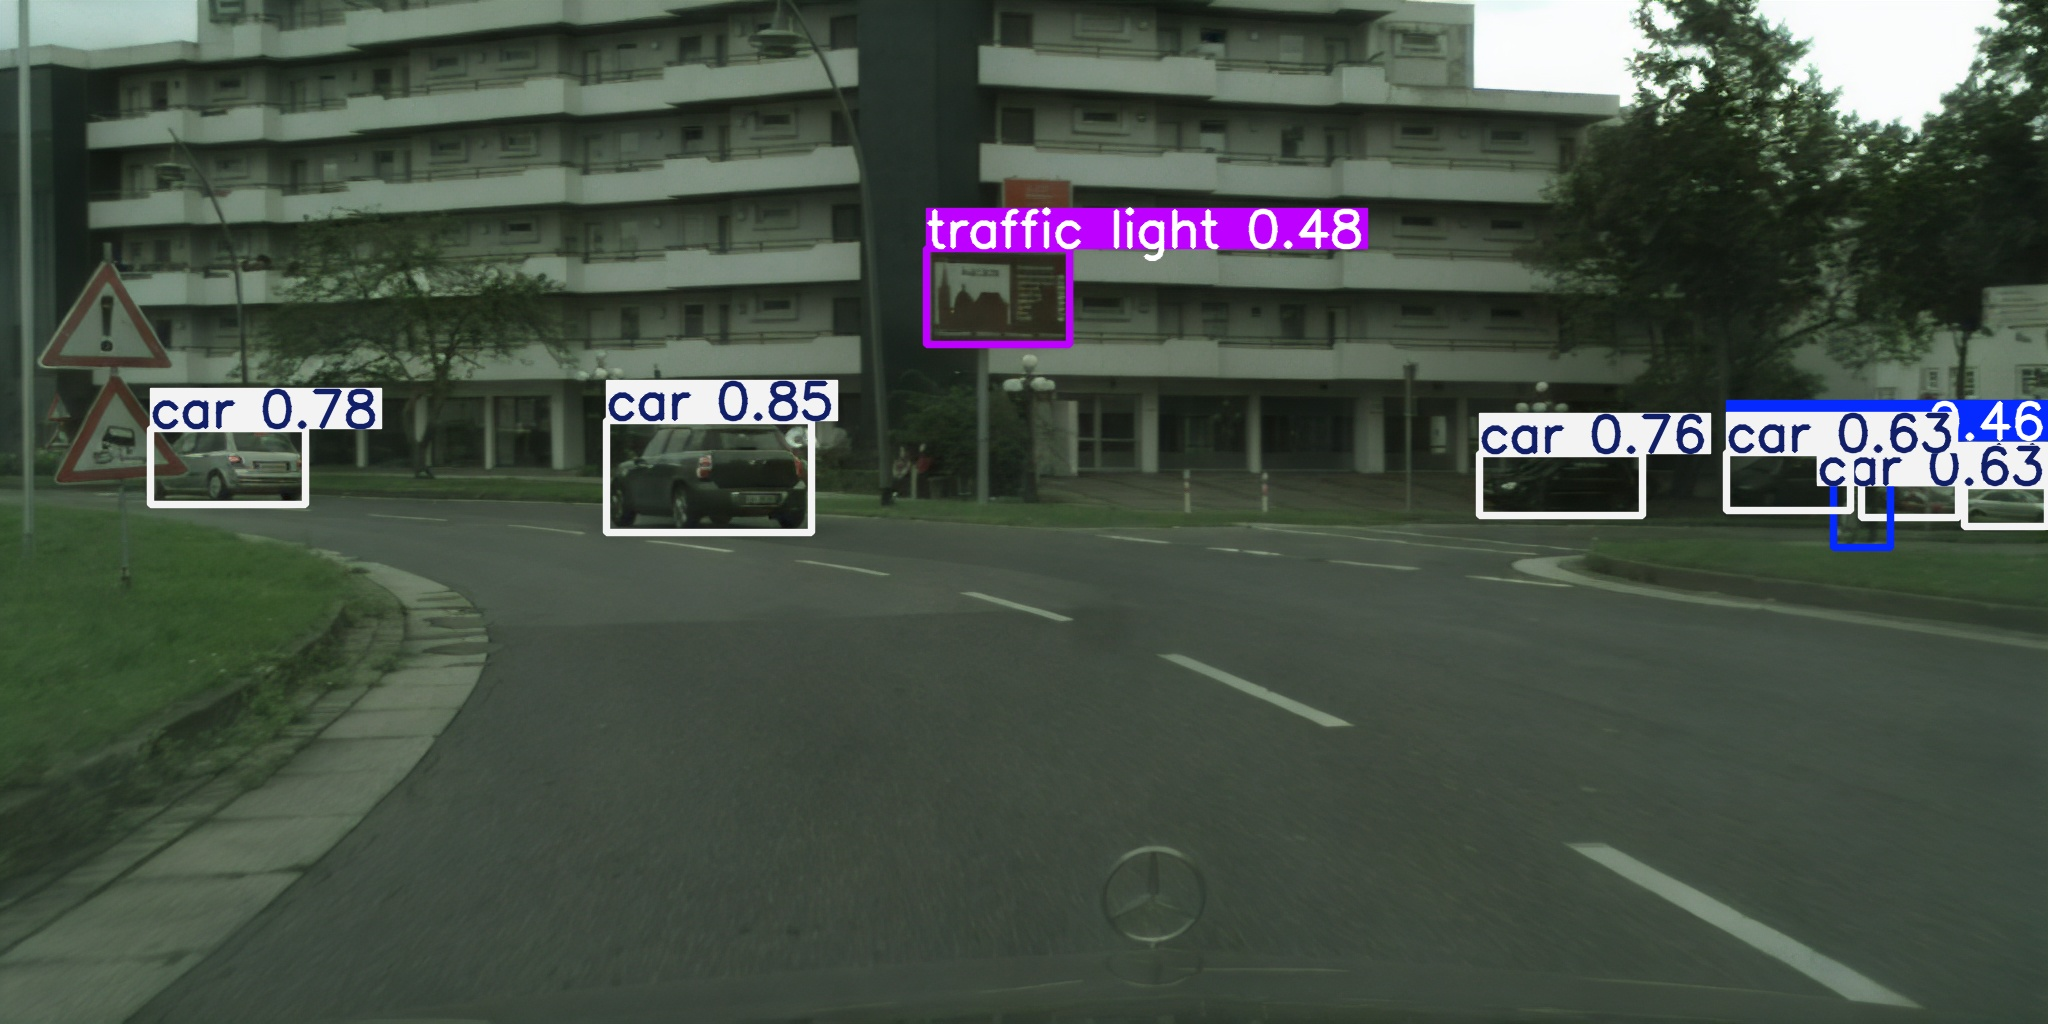
\includegraphics[scale=0.19]{pictures/vq-f8-n256_aachen_000000.jpg}
                \caption{Rekonstruiertes Bild durch das vq-f8-n256-Modell (Aachen, erstes Bild), verarbeitet zur Objekterkennung durch das YOLO-Modell.}
                \label{fig:vq-f8-n256_aachen_000000}
            \end{figure}
            \begin{figure}[!htb]
                \centering
                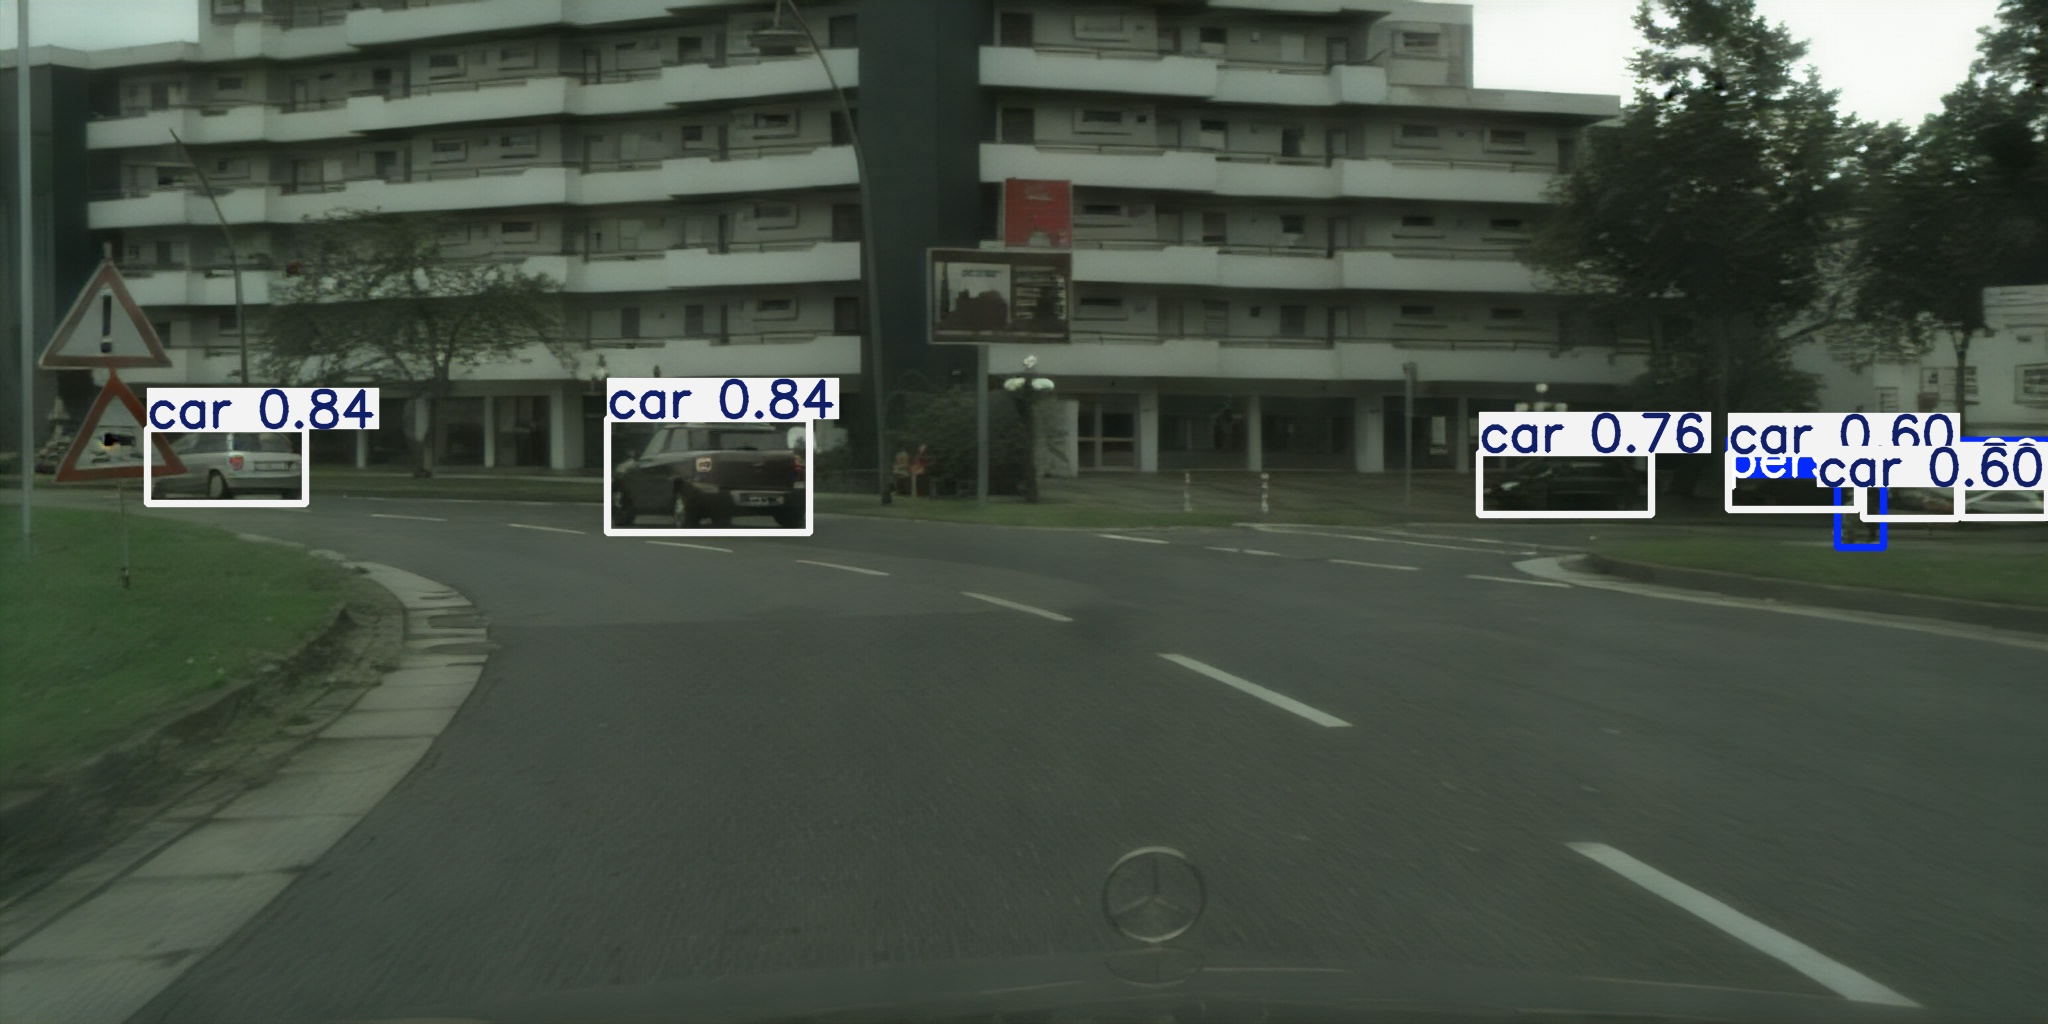
\includegraphics[scale=0.19]{pictures/vq-f16_aachen_000000.jpg}
                \caption{Rekonstruiertes Bild durch das vq-f16-Modell (Aachen, erstes Bild), verarbeitet zur Objekterkennung durch das YOLO-Modell.}
                \label{fig:vq-f16_aachen_000000}
            \end{figure}
\newpage
            \begin{figure}[!htb]
                \centering
                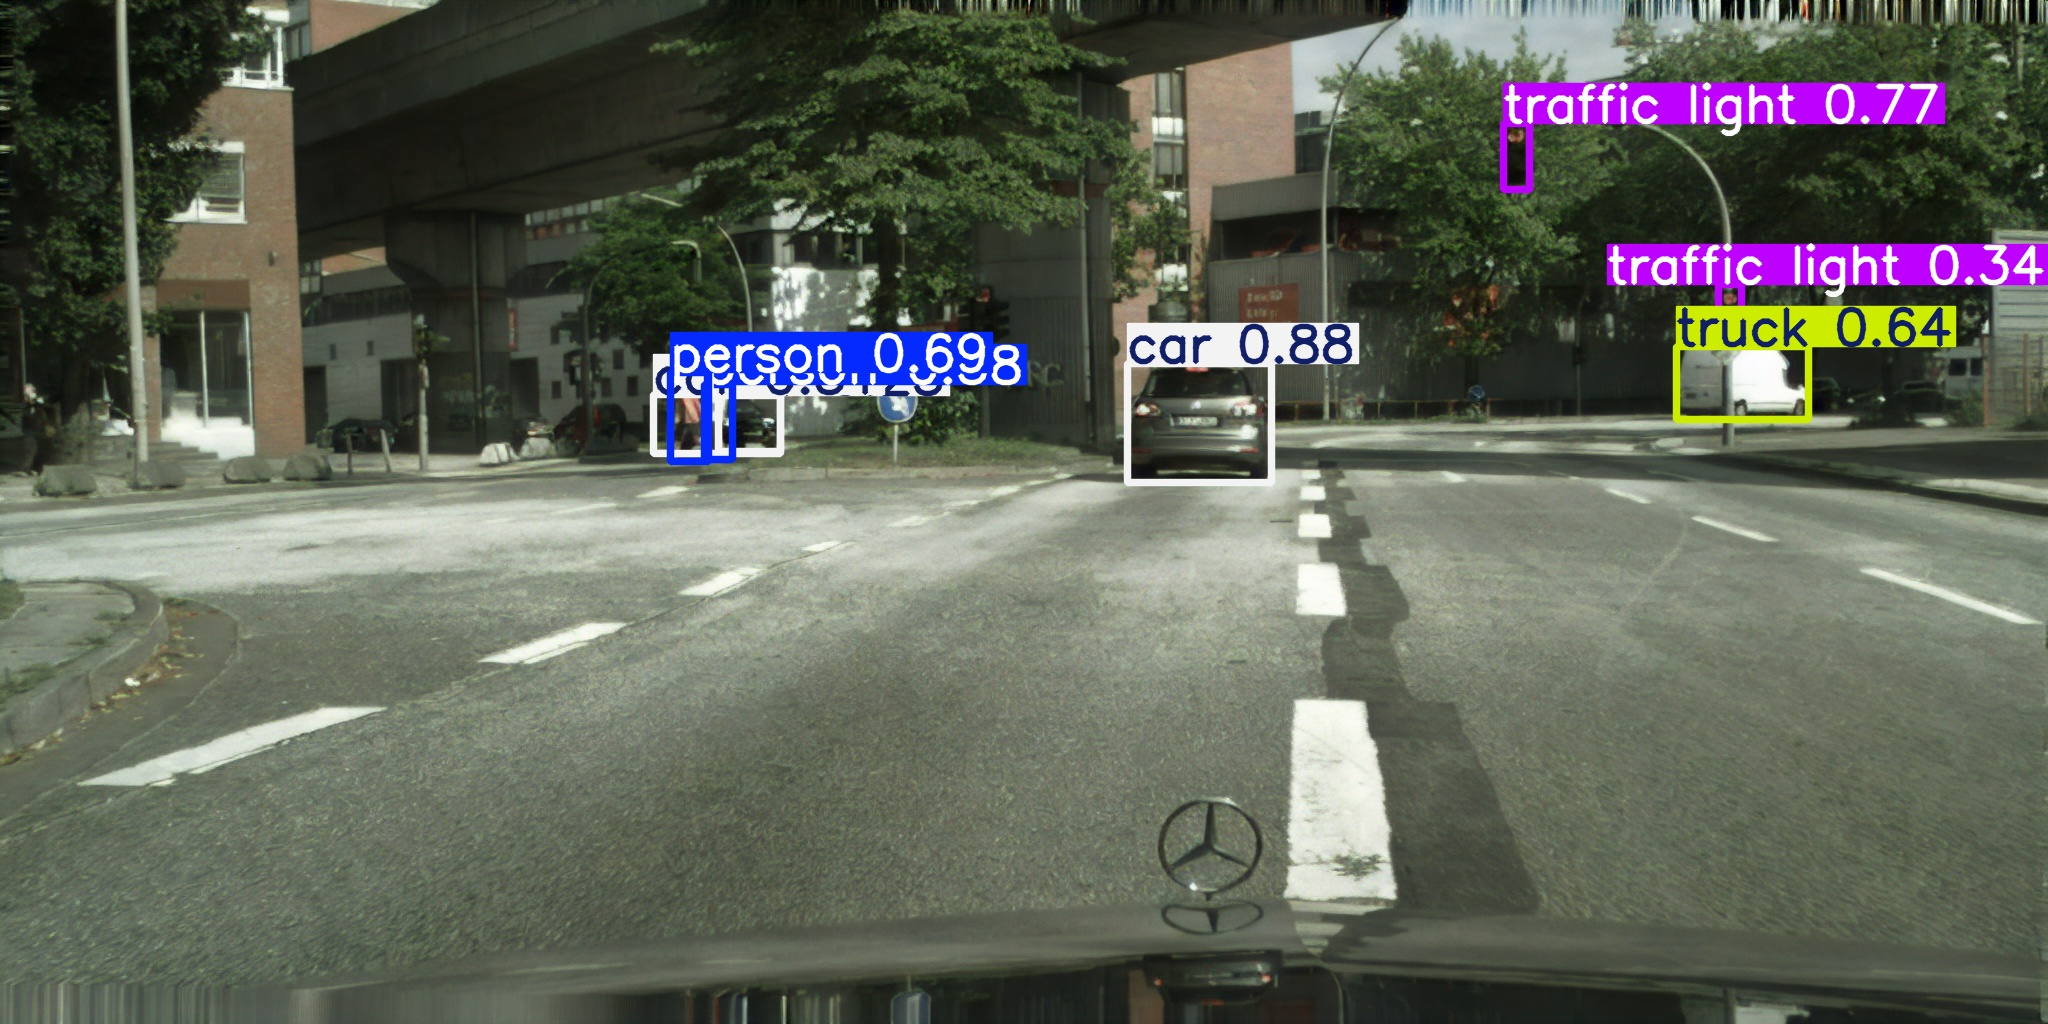
\includegraphics[scale=0.19]{pictures/vq-f8-n256_hamburg_000000.jpg}
                \caption{Rekonstruiertes Bild durch das vq-f8-n256-Modell (Hamburg, sechstes Bild), verarbeitet zur Objekterkennung durch das YOLO-Modell.}
                \label{fig:vq-f8-n256_hamburg_000000}
            \end{figure}
            \begin{figure}[!htb]
                \centering
                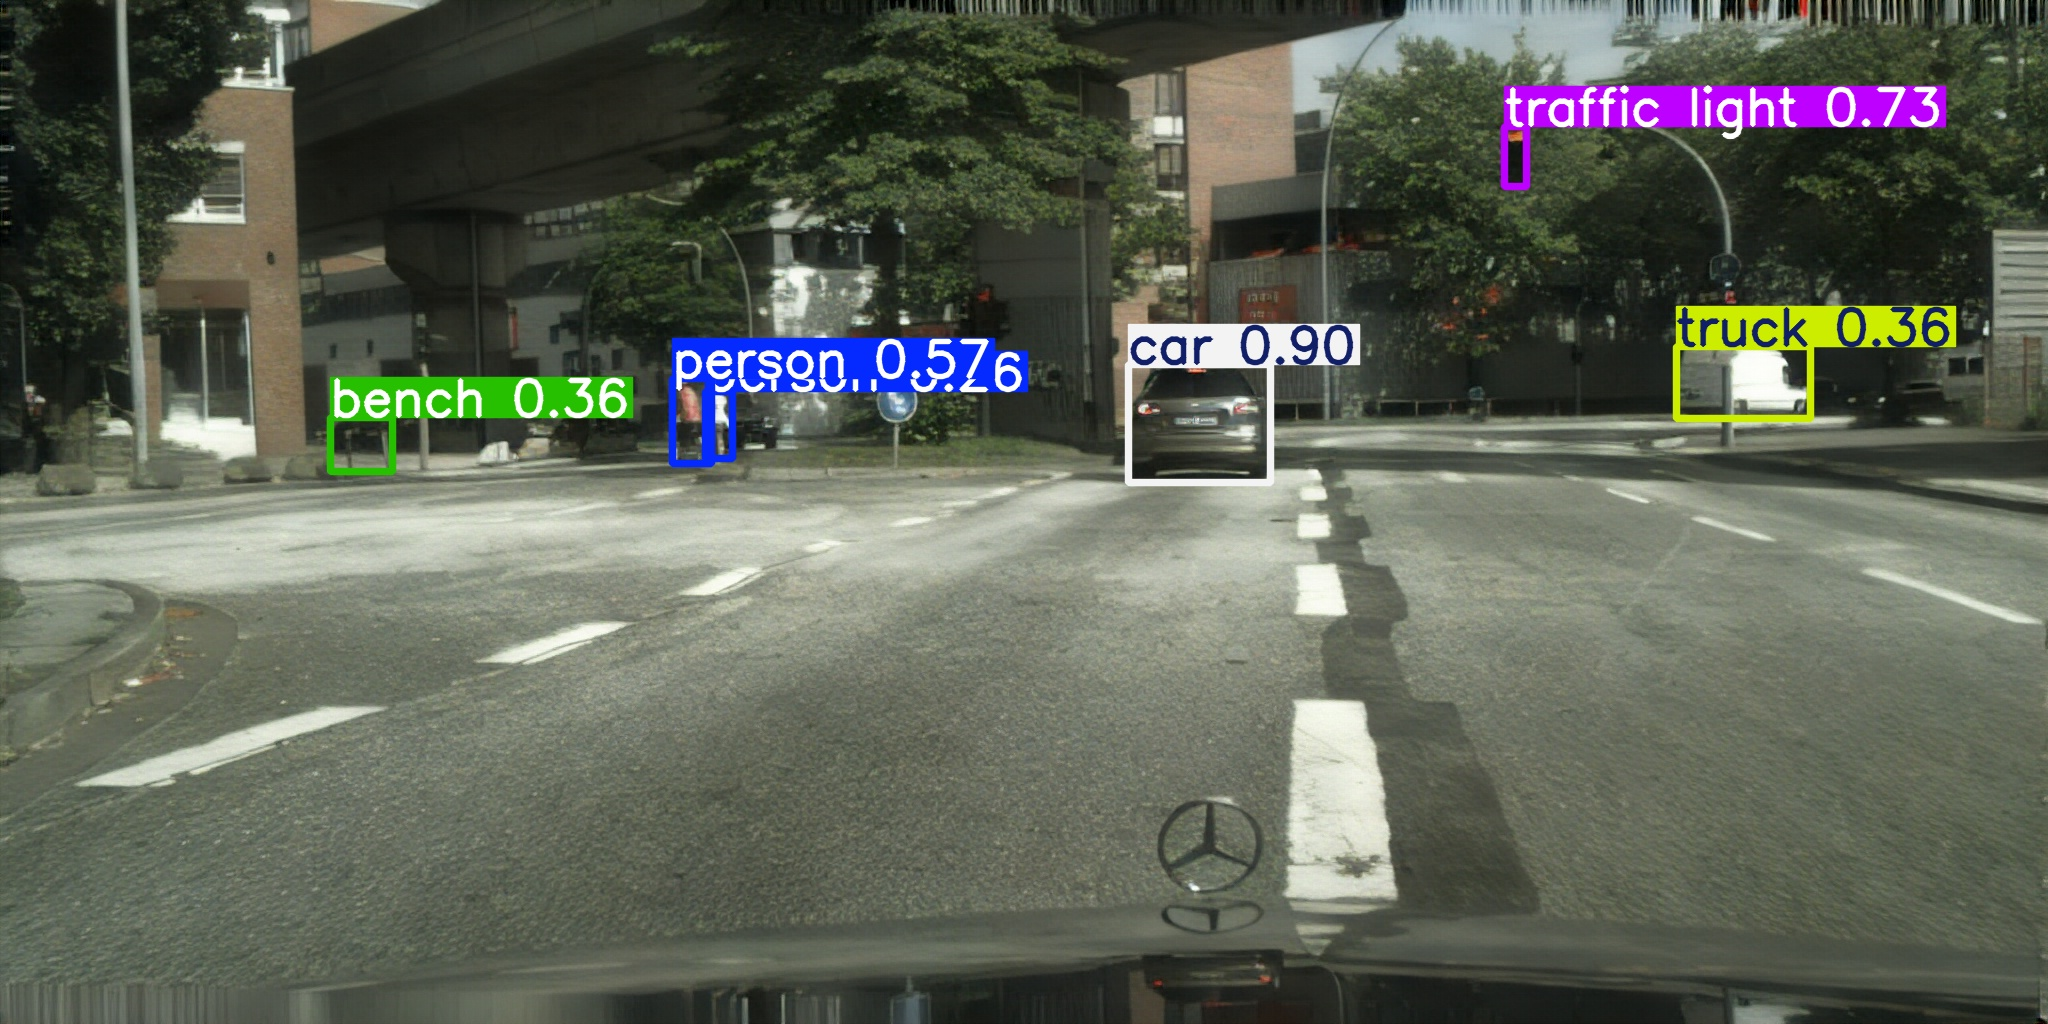
\includegraphics[scale=0.19]{pictures/vq-f16_hamburg_000000.jpg}
                \caption{Rekonstruiertes Bild durch das vq-f16-Modell (Hamburg, sechstes Bild), verarbeitet zur Objekterkennung durch das YOLO-Modell.}
                \label{fig:vq-f16_000000}
            \end{figure}

\newpage
            Auf beiden Aachen-Bildern, Abbildungen \ref{fig:vq-f8-n256_aachen_000000} und \ref{fig:vq-f16_aachen_000000}, werden alle Autos erkannt sowie eine Person. Im Vergleich zum Ground-Truth-Label-Bild
            (Abbildung \ref{fig:og_aachen_000000}) wird auf beiden eine Person nicht erkannt, sowie fälschlicherweise ein Schild als „traffic light“ klassifiziert \ref{fig:vq-f8-n256_aachen_000000}, welches vom
            \textbf{vq-f8-n256}-Modell rekonstruiert wurde.
            Obwohl die Bilder eindeutig dem Original sehr ähneln, kann das YOLO-Modell nicht alle Label-Objekte des Originals in den rekonstruierten Bildern detektieren.
            Auf den Hamburg-Bildern, Abbildung \ref{fig:vq-f8-n256_hamburg_000000} und \ref{fig:vq-f16_000000},
            sieht man mehr Unterschiede. Das YOLO-Modell erkennt auf den \textbf{vq-f8-n256}-Bildern beide
            „traffic light“ sowie zwei „Car“-Objekte, wohingegen das \textbf{vq-f16} rekonstruierte Bild mit lediglich einem  
            „car“ und einem „traffic light“ sowie einer Falschklassifizierung deutlich schlechter abschneidet, wenn man beide Bilder mit dem Originalen vergleicht, Abbildung \ref{fig:og_hamburg_6}.
            
            Dies ist bei den meisten Vergleichen der Fall, wenn man \textbf{vq-f16} und \textbf{vq-f8-n256}-Bilder mit Boundingboxen untersucht. Es kommt bei den \textbf{vq-f16}-Bildern häufiger zu Fehlklassifizierungen. Häufig werden „car“-Objekte als „truck“-Objekte bei mangelnder Qualität klassifiziert, oder „traffic light“-Objekte werden nicht wiedererkannt.\\
            \textbf{vq-f8-n256} \ref{fig:vq-f8-n256_hamburg_000000}:\\
            $\text{true positives} = 7 \quad \text{false positives} = 0 \quad \text{false negatives} = 1$\\
            \textbf{vq-f16} \ref{fig:vq-f16_000000}:\\
            $\text{true positives} = 5 \quad \text{false positives} = 1 \quad \text{false negatives} = 3$
            
            
            
\newpage  
            \underline{\textbf{Metriken zum Vergleich von Bildern mit Labels}}  

            \begin{figure}[!htb]
                \centering
                \includesvg[scale=0.56]{graphs/output_plot_f1_pr_re_model.svg}
                \caption{Diese Grafik zeigt die Metriken Precison, Recall und F1 Score in Abhängigkeit zur Kompressionsqualität.}
                \label{fig:pr_f1_re_model}
            \end{figure}

            Die Grafik zeigt anders als \ref{fig:pr_f1_re} nun auch die beiden Modelle in Abhängigkeit vom Kompressionsfaktor. Die Metriken weisen deutliche Qualitätsunterschiede untereinander zwischen den Modellen auf. Während die Differenz bei Precision lediglich $0,0043$ beträgt, liegt sie beim F1-Score bereits bei $0,0396$ und bei Recall sogar bei einem Wert von $0.0666$.
            Auffällig ist, dass der F1-Score des \textbf{vq-f16}-Modells nahezu identisch mit dem Recall des \textbf{vq-f8-n256}-Modells ist.
            Zudem bewegen sich Recall und F1-Score des \textbf{vq-f16}-Modells im Bereich einer JPEG-Kompressionsqualität von $15\%$ bis $20\%$, während diese Werte für das \textbf{vq-f8-n256} zwischen
            $25\%$ und $30\%$ liegen. Precision hingegen zeigt bei beiden Modellen nahezu identische Werte, die ungefähr einer JPEG-Kompressionsqualität von $25\%$ entsprechen.
            
\newpage        
            Der Grund, weshalb die Differenz der Precision der beiden Modelle so gering ist, liegt an der Art der Berechnung.
            \begin{center}  
                \large$prescicion = \frac{\text{true positives}}{\text{true positives} + \text{false positives}}$\\
            \end{center}
            Es werden lediglich \text{true positives} und \text{false positives} für die Berechnung verwendet.
            Das YOLO-Modell muss also auf den rekonstruierten Bildern Boundingboxen richtig erkennen und so wenig wie möglich falsche neue Boundingboxen erstellen. Jedoch spielt es keinen Faktor in die Berechnung der Precision, ob Boundingboxen aufgrund mangelnder Bildqualität gar nicht erst erkannt\\
            werden (false negatives).\vspace{2mm}
            
            \noindent\textbf{vq-f8-n256}-Datensatz:\\
            $\text{true positives} = 31697 \quad \text{false positives} = 1615 \quad \text{false negatives} = 4799$\\
            \textbf{vq-f16}-Datensatz:\\
            $\text{true positives} = 29266 \quad \text{false positives} = 1630 \quad \text{false negatives} = 7230$\\

            Während ein deutlicher Unterschied zwischen \text{true positives} und \text{false negatives} besteht, beträgt die Differenz der \text{false positives} lediglich $15$. Dies zeigt, dass das YOLO-Modell in beiden Modelldatensätzen Boundingboxen erzeugt hat, die im Original nicht existieren – ein Beispiel hierfür ist die „bench“ in Abbildung \ref{fig:vq-f16_000000}. Allerdings tritt dieser Fall nur selten auf, wie die Zahlen verdeutlichen, und es gibt kaum Unterschiede zwischen den beiden Modellen.

            Was das Original (\ref{fig:og_hamburg_6}) im Vergleich zu den beiden rekonstruierten Bildern erneut aufweist, ist, dass die Wahrscheinlichkeiten der erkannten Objekte in Abbildung \ref{fig:vq-f8-n256_hamburg_000000} des \textbf{vq-f8-n256} besser sind. Lediglich das „car“-Objekt weist in dem durch den \textbf{vq-f16} rekonstruierten Bild einen besseren Wert auf, sogar besser als der Wert im Originalen.
            Ein weiterer Beweis, der zeigt, dass auch das Modell, welches die Objekte detektiert, eine Rolle spielt, was die Qualität der Metrikwerte betrifft.
            
\newpage  
            \underline{\textbf{Intersection over Union (IoU)}}

            \begin{figure}[!htb]
                \centering
                \includesvg[scale=0.56]{graphs/output_plot_iou_model.svg}
                \caption{IoU in Abhängigkeit zum Kompressionsfaktor.}
                \label{fig:iou_model}
            \end{figure}

            Der IoU der beiden Modelle weist eine Differenz von $0.0859$ auf. Während die Performance des \textbf{vq-f8-n256}-Modells bei Kompressionsqualitäten zwischen $25\%$ und $30\%$ liegt, befindet sich das \textbf{vq-f16}-Modell leistungstechnisch im Bereich von $15\%$ und $20\%$. Dies entspricht den Ergebnissen von Recall und F1-Score aus Abbildung \ref{fig:pr_f1_re_model}.
            Somit zeigen sich Übereinstimmungen zwischen den Kompressionsqualitäten der JPEG-Daten sowie den IoU-, Recall- und F1-Werten der Modelle in Abhängigkeit vom Kompressionsfaktor. 
            Alle drei Metriken liegen bei beiden Modellen durchgehend innerhalb der Wertebereiche der entsprechenden JPEG-Datensätze, abhängig von der Kompressionsqualität. Ähnliches war bereits bei Metriken wie SSIM, MSE und PSNR zu beobachten, bei denen die Modelle ebenfalls stets innerhalb der gleichen Kompressionsqualitätsstufen der JPEG-Datensätze lagen.
            

\newpage 
            \begin{figure}[!htb]
                \centering
                \includesvg[scale=0.56]{graphs/output_plot_iou_std_model.svg}
                \caption{IoU in Abhängigkeit zum Kompressionsfaktor mit Standartabweichung.}
                \label{fig:iou_std_model}
            \end{figure}  
            
            In Abbildung \ref{fig:iou_std_model} ist zu erkennen, dass die Standardabweichung der beiden Modelle sehr hoch ist, ähnlich wie bei den JPEG-Datensätzen. Das \textbf{vq-f8-n256}-Modell weist eine Standardabweichung von $0.3165$ auf, während das \textbf{vq-f16}-Modell eine Standardabweichung von $0.3693$ hat.
            Auch dies ist auf die vielen Werte über $0,5$ und die Werte, die auf $0,0$ gesetzt wurden, zurückzuführen. Nicht nur der IoU-Wert, sondern auch die Standardabweichung der jeweiligen Modelle liegt bei \textbf{vq-f8-n256} zwischen Kompressionsqualitäten von $25\%$ und $30\%$. Bei \textbf{vq-f16} befindet sich die Standardabweichung zwischen $15\%$ und $20\%$. Sowohl die Standardabweichung als auch der IoU-Wert sind in gleicher Weise vom Kompressionsfaktor abhängig.
            Die beiden Modelle sind untereinander was den IoU-Wert betrifft $0,086$ Einheihten auseinander und bei der Standartabweichung um $0,053$.
            Dies ist in etwa die Gleiche Differenz wie bei den Kopressionsqualitäten von $15\%$ und $20\%$ der Fsll ist.
            Egal welche Metrik man Untersucht die Modelle und ihre Werte spielen sich meist immer in den selben Bereichen, $25\%$ und $30\%$ bei \textbf{vq-f8-n256}-Modell und $15\%$ und $20\%$ bei \textbf{vq-f16}-Modell, ab. Es zeigt das es zwischen allen Metriken stets Gleichheiten gibt und diese Gleichheiten
            Abhängig sind vom Kompressionsfaktor.
            
\chapter{Fazit}
    Die Arbeit zeigt, dass zwischen den KI-Daten und den JPEG-Daten wiederholt Übereinstimmungen auftreten, etwa beim Abschneiden der Modelle im Vergleich zu den Metriken der JPEG-Datensätze. Auch die Metriken untereinander zeigen konsistente Übereinstimmungen in Abhängigkeit vom Kompressionsfaktor. Es bestehen Abhängigkeiten zwischen der Bildqualität und dem Kompressionsfaktor sowie Kausalitäten, die darauf hindeuten, dass Bilder mit geringerer Qualität zu schlechteren Ergebnissen in der Objekterkennung führen.
    
    Als abschließendes Fazit dieser Arbeit lässt sich feststellen, dass es in der Praxis möglich ist, Bilder so zu komprimieren, dass Bandbreite eingespart werden kann, um Bilder zu übertragen. Allerdings zeigt die Arbeit auch, dass die Performance von Modellen, welche auf rekonstruierten Daten Vorhersagen treffen sollen, maßgeblich von zwei Hauptfaktoren abhängt.
    
    Zum einen muss die Qualität des komprimierten Bildes nahezu identisch zum Original bleiben, d.h. ein SSIM-Wert, welcher den Wert $1,0$ approximiert. Dies ist mit traditionellen Kompressionsverfahren wie JPEG nicht zu erreichen, wenn gleichzeitig ein hoher Kompressionsgrad angestrebt wird, wie Kompressionsfaktoren von $50+$ aufwärts. Hierfür sind lernbasierte Kompressionsverfahren erforderlich. Allerdings steht auch bei diesen Verfahren eine zu starke Kompression in direktem Konflikt mit dem Qualitätsverlust des Bildes. 
    Metriken wie SSIM haben gezeigt, dass KI-basierte komprimierte und rekonstruierte Bilder in Bezug auf Kontrast, Struktur und Helligkeit deutlich bessere Ergebnisse liefern als JPEG-komprimierte Bilder, was deren Qualität betrifft. 

    Der zweite Hauptfaktor liegt im Modell, das nachträglich auf den Bildern eingesetzt wird. Obwohl in dieser Arbeit alle Bilder mit demselben Modell evaluiert werden, treten dennoch deutliche Diskrepanzen auf. Das Modell, das mit den Daten gespeist wird, muss ausreichend auf diese Art von Daten trainiert werden und über passende Features und Labels verfügen. In diesem Fall ist ein YOLO-Modell, das speziell auf Cityscapes-Daten trainiert wird, robuster gegenüber solchen Diskrepanzen. Auch hier gibt es einen kausalen Zusammenhang zwischen dem Modell, welches für die Objektdetektion zuständig ist, und der Genauigkeit der Vorhersagen.

\newpage
    Da es beim autonomen Fahren um Menschenleben geht, müssen Modelle zur Einsparung von Bandbreite auch anhand weiterer Metriken genauestens evaluiert werden, ob diese auch den Ansprüchen gerecht werden und mit den zur Domäne passenden Daten ausreichend trainiert wurden.
    Zur Evaluation sollten zudem Metriken angewandt werden, welche die menschliche Wahrnehmung berücksichtigen. Unter keinen Umständen darf die Bildqualität zugunsten von Bandbreite und Speicherplatz geopfert werden. Modelle mit niedrigeren Kompressionsfaktoren, beispielsweise $50$ statt $219,43$ oder $192$, erzielen deutlich bessere Ergebnisse, da mehr Informationen im latenten Raum zur Rekonstruktion zur Verfügung stehen.
    Die beiden getesteten Modelle haben wertvolle Einblicke in die Möglichkeiten und das Potenzial lernbasierter Kompression geliefert, sind jedoch für eine sicherheitskritische Domäne wie das autonome Fahren ungeeignet, da sie in ihrer Performance deutlich zu schwach abschneiden.

    In der Zukunft des autonomen Fahrens werden KI-Modelle zum Einsatz kommen,
    um in Bandbreite und Speicherkapazitäten zu sparen – vorausgesetzt, die beiden Hauptfaktoren werden dabei berücksichtigt.
    
    
\part{Anhang}

\section*{Prozentuale Speichergröße abhängig zur Kompressionsqualität}
\begin{itemize}
    \item Durchschn. Gr. [\%] = 1.7753, Var (0.0116), Std (0.1079), Kompression 5
    \item Durchschn. Gr. [\%] = 2.2008, Var (0.0454), Std (0.2131), Kompression 10
    \item Durchschn. Gr. [\%] = 2.5956, Var (0.0925), Std (0.3042), Kompression 15
    \item Durchschn. Gr. [\%] = 2.9598, Var (0.1483), Std (0.3852), Kompression 20
    \item Durchschn. Gr. [\%] = 3.3149, Var (0.2125), Std (0.4609), Kompression 25
    \item Durchschn. Gr. [\%] = 3.6475, Var (0.2803), Std (0.5294), Kompression 30
    \item Durchschn. Gr. [\%] = 4.2521, Var (0.4210), Std (0.6489), Kompression 40
    \item Durchschn. Gr. [\%] = 4.8640, Var (0.5814), Std (0.7625), Kompression 50
    \item Durchschn. Gr. [\%] = 5.5362, Var (0.7793), Std (0.8828), Kompression 60
    \item Durchschn. Gr. [\%] = 6.6223, Var (1.1183), Std (1.0575), Kompression 70
    \item Durchschn. Gr. [\%] = 7.3122, Var (1.3500), Std (1.1619), Kompression 75
    \item Durchschn. Gr. [\%] = 10.0661, Var (2.3375), Std (1.5289), Kompression 85
    \item Durchschn. Gr. [\%] = 13.0879, Var (3.5185), Std (1.8758), Kompression 90
    \item Durchschn. Gr. [\%] = 20.1317, Var (6.6612), Std (2.5809), Kompression 95
    \item Durchschn. Gr. [\%] = 49.6575, Var (19.2566), Std (4.3882), Kompression 100
\end{itemize}


\newpage
\section*{Kompressionsfaktor abhängig zur Kompressionsqualität}

\begin{itemize}
    \item Faktor = 56.3271, Var (11.7193), Std (3.4233), Kompression 5
    \item Faktor = 45.4375, Var (19.3515), Std (4.3990), Kompression 10
    \item Faktor = 38.5274, Var (20.3912), Std (4.5157), Kompression 15
    \item Faktor = 33.7861, Var (19.3303), Std (4.3966), Kompression 20
    \item Faktor = 30.1667, Var (17.5956), Std (4.1947), Kompression 25
    \item Faktor = 27.4159, Var (15.8330), Std (3.9791), Kompression 30
    \item Faktor = 23.5180, Var (12.8794), Std (3.5888), Kompression 40
    \item Faktor = 20.5591, Var (10.3865), Std (3.2228), Kompression 50
    \item Faktor = 18.0628, Var (8.2953), Std (2.8801), Kompression 60
    \item Faktor = 15.1006, Var (5.8148), Std (2.4114), Kompression 70
    \item Faktor = 13.6758, Var (4.7222), Std (2.1731), Kompression 75
    \item Faktor = 9.9343, Var (2.2767), Std (1.5089), Kompression 85
    \item Faktor = 7.6407, Var (1.1992), Std (1.0951), Kompression 90
    \item Faktor = 4.9673, Var (0.4055), Std (0.6368), Kompression 95
    \item Faktor = 2.0138, Var (0.0317), Std (0.1780), Kompression 100
\end{itemize}


\newpage
\section*{SSIM, PSNR, MSE Werte}
        \begin{table}[h!]
\centering
\begin{tabular}{|c|c|c|c|}
\hline
\textbf{Kompression} & \textbf{SSIM} & \textbf{PSNR} & \textbf{MSE} \\ \hline
5                    & 0.6345        & 75.7594       & 0.001747     \\ \hline
10                   & 0.8007        & 79.1075       & 0.000807     \\ \hline
15                   & 0.8876        & 81.4212       & 0.000477     \\ \hline
20                   & 0.9229        & 83.0211       & 0.000333     \\ \hline
25                   & 0.9359        & 83.9889       & 0.000268     \\ \hline
30                   & 0.9412        & 84.5488       & 0.000236     \\ \hline
40                   & 0.9533        & 85.6218       & 0.000185     \\ \hline
50                   & 0.9613        & 86.4335       & 0.000154     \\ \hline
60                   & 0.9646        & 86.9647       & 0.000137     \\ \hline
70                   & 0.9697        & 87.7416       & 0.000115     \\ \hline
75                   & 0.9730        & 88.2414       & 0.000103     \\ \hline
85                   & 0.9779        & 89.3331       & 0.000080     \\ \hline
90                   & 0.9811        & 90.1780       & 0.000065     \\ \hline
95                   & 0.9853        & 91.6023       & 0.000047     \\ \hline
100                  & 0.9938        & 95.7158       & 0.000018     \\ \hline
vq-f16               & 0.8769        & 76.5315       & 0.001559     \\ \hline
vq-f8-n256           & 0.9020        & 78.4603       & 0.000987     \\ \hline
\end{tabular}
\caption{Übersicht der Kompressionswerte mit SSIM, PSNR und MSE.}
\label{tab:compression}
\end{table}

\newpage
\section*{Precisiom, Recall, F1-Score Werte}
\begin{table}[h!]
\centering
\begin{tabular}{|c|c|c|c|}
\hline
\textbf{Kompression} & \textbf{Precision} & \textbf{Recall} & \textbf{F1} \\ \hline
5                    & 0.7965             & 0.4856          & 0.6034      \\ \hline
10                   & 0.8543             & 0.6439          & 0.7343      \\ \hline
15                   & 0.9144             & 0.7710          & 0.8366      \\ \hline
20                   & 0.9383             & 0.8372          & 0.8849      \\ \hline
25                   & 0.9488             & 0.8642          & 0.9045      \\ \hline
30                   & 0.9553             & 0.8774          & 0.9147      \\ \hline
40                   & 0.9611             & 0.8996          & 0.9293      \\ \hline
50                   & 0.9652             & 0.9127          & 0.9382      \\ \hline
60                   & 0.9677             & 0.9185          & 0.9424      \\ \hline
70                   & 0.9708             & 0.9274          & 0.9486      \\ \hline
75                   & 0.9724             & 0.9343          & 0.9530      \\ \hline
85                   & 0.9750             & 0.9463          & 0.9604      \\ \hline
90                   & 0.9755             & 0.9530          & 0.9641      \\ \hline
95                   & 0.9777             & 0.9638          & 0.9707      \\ \hline
100                  & 0.9802             & 0.9749          & 0.9775      \\ \hline
vq-f16              & 0.9472             & 0.8019          & 0.8685      \\ \hline
vq-f8-n256         & 0.9515             & 0.8685          & 0.9081      \\ \hline
\end{tabular}
\caption{Übersicht der Kompressionswerte mit Precision, Recall und F1-Score.}
\label{tab:compression_metrics}
\end{table}

\newpage
    \section*{Durchschnittliche IoU-Werte und Statistiken}

\begin{itemize}
    \item Durchschn. IoU = 0.4467, Var (0.1901), Std (0.4360), Kompression 5
    \item Durchschn.  IoU = 0.5737, Var (0.1753), Std (0.4187), Kompression 10
    \item Durchschn.  IoU = 0.6772, Var (0.1461), Std (0.3822), Kompression 15
    \item Durchschn.  IoU = 0.7514, Var (0.1176), Std (0.3429), Kompression 20
    \item Durchschn.  IoU = 0.7916, Var (0.1007), Std (0.3173), Kompression 25
    \item Durchschn.  IoU = 0.8135, Var (0.0913), Std (0.3021), Kompression 30
    \item Durchschn.  IoU = 0.8439, Var (0.0769), Std (0.2774), Kompression 40
    \item Durchschn.  IoU = 0.8648, Var (0.0667), Std (0.2584), Kompression 50
    \item Durchschn.  IoU = 0.8757, Var (0.0626), Std (0.2502), Kompression 60
    \item Durchschn.  IoU = 0.8901, Var (0.0550), Std (0.2345), Kompression 70
    \item Durchschn.  IoU = 0.9004, Var (0.0497), Std (0.2229), Kompression 75
    \item Durchschn.  IoU = 0.9193, Var (0.0397), Std (0.1993), Kompression 85
    \item Durchschn.  IoU = 0.9293, Var (0.0346), Std (0.1859), Kompression 90
    \item Durchschn.  IoU = 0.9442, Var (0.0263), Std (0.1621), Kompression 95
    \item Durchschn.  IoU = 0.9609, Var (0.0174), Std (0.1319), Kompression 100
    \item Durchschn.  IoU = 0.7951, Var (0.1002), Std (0.3165), Kompression vq-f8-f256
    \item Durchschn.  IoU = 0.7092, Var (0.1364), Std (0.3693), Kompression vq-f16
\end{itemize}

\part{Anhang}
\section*{Latente Darstellung des vq-f16-Modells (Aachen erstes Bild)}
     
            \begin{figure}[!htb]
                \centering
                \begin{minipage}[!htb]{0.47\textwidth}
                    \centering
                    \textbf{Kanal 1} % Überschrift für die erste Spalte
                \end{minipage}
                %
                \begin{minipage}[!htb]{0.47\textwidth}
                    \centering
                    \textbf{Kanal 2} % Überschrift für die zweite Spalte
                \end{minipage}
    
                \begin{minipage}[!htb]{0.48\textwidth}
                    \centering
                    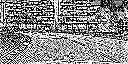
\includegraphics[width=\textwidth]{pictures/vq-f16_latent_channel_1.png}    
                \end{minipage}
                %
                \begin{minipage}[!htb]{0.48\textwidth}
                    \centering
                    
\includegraphics[width=\textwidth]{pictures/vq-f16_latent_channel_2.png}
                \end{minipage}
            \end{figure}
            \begin{figure}[!htb]
                \centering
                \begin{minipage}[!htb]{0.47\textwidth}
                    \centering
                    \textbf{Kanal 3} % Überschrift für die erste Spalte
                \end{minipage}
                %
                \begin{minipage}[!htb]{0.47\textwidth}
                    \centering
                    \textbf{Kanal 4} % Überschrift für die zweite Spalte
                \end{minipage}
    
                \begin{minipage}[!htb]{0.48\textwidth}
                    \centering
                    
\includegraphics[width=\textwidth]{pictures/vq-f16_latent_channel_3.png}    
                \end{minipage}
                %
                \begin{minipage}[!htb]{0.48\textwidth}
                    \centering
                    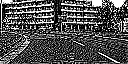
\includegraphics[width=\textwidth]{pictures/vq-f16_latent_channel_4.png}
                \end{minipage}
            \end{figure}
            \begin{figure}[!htb]
                \centering
                \begin{minipage}[!htb]{0.47\textwidth}
                    \centering
                    \textbf{Kanal 5} % Überschrift für die erste Spalte
                \end{minipage}
                %
                \begin{minipage}[!htb]{0.47\textwidth}
                    \centering
                    \textbf{Kanal 6} % Überschrift für die zweite Spalte
                \end{minipage}
    
                \begin{minipage}[!htb]{0.48\textwidth}
                    \centering
                    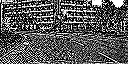
\includegraphics[width=\textwidth]{pictures/vq-f16_latent_channel_5.png}    
                \end{minipage}
                %
                \begin{minipage}[!htb]{0.48\textwidth}
                    \centering
                    
\includegraphics[width=\textwidth]{pictures/vq-f16_latent_channel_6.png}
                \end{minipage}
            \end{figure}
            \begin{figure}[!htb]
                \centering
                \begin{minipage}[!htb]{0.47\textwidth}
                    \centering
                    \textbf{Kanal 7} % Überschrift für die erste Spalte
                \end{minipage}
                %
                \begin{minipage}[!htb]{0.47\textwidth}
                    \centering
                    \textbf{Kanal 8} % Überschrift für die zweite Spalte
                \end{minipage}
    
                \begin{minipage}[!htb]{0.48\textwidth}
                    \centering
                    
\includegraphics[width=\textwidth]{pictures/vq-f16_latent_channel_7.png}    
                \end{minipage}
                %
                \begin{minipage}[!htb]{0.48\textwidth}
                    \centering
                    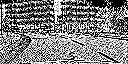
\includegraphics[width=\textwidth]{pictures/vq-f16_latent_channel_8.png}
                \end{minipage}
            \end{figure}
            
\newpage
\section*{Latente Darstellung des vq-f8-n256-Modells (Aachen erstes Bild)}
     
            \begin{figure}[!htb]
                \centering
                \begin{minipage}[!htb]{0.47\textwidth}
                    \centering
                    \textbf{Kanal 1} % Überschrift für die erste Spalte
                \end{minipage}
                %
                \begin{minipage}[!htb]{0.47\textwidth}
                    \centering
                    \textbf{Kanal 2} % Überschrift für die zweite Spalte
                \end{minipage}
    
                \begin{minipage}[!htb]{0.48\textwidth}
                    \centering
                    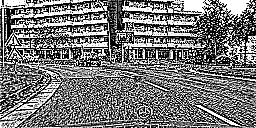
\includegraphics[width=\textwidth]{pictures/vq-f8-n256_latent_channel_1.png}    
                \end{minipage}
                %
                \begin{minipage}[!htb]{0.48\textwidth}
                    \centering
                    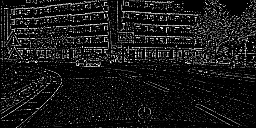
\includegraphics[width=\textwidth]{pictures/vq-f8-n256_latent_channel_2.png}
                \end{minipage}
            \end{figure}
            \begin{figure}[!htb]
                \centering
                \begin{minipage}[!htb]{0.47\textwidth}
                    \centering
                    \textbf{Kanal 3} % Überschrift für die erste Spalte
                \end{minipage}
                %
                \begin{minipage}[!htb]{0.47\textwidth}
                    \centering
                    \textbf{Kanal 4} % Überschrift für die zweite Spalte
                \end{minipage}
    
                \begin{minipage}[!htb]{0.48\textwidth}
                    \centering
                    
\includegraphics[width=\textwidth]{pictures/vq-f8-n256_latent_channel_3.png}    
                \end{minipage}
                %
                \begin{minipage}[!htb]{0.48\textwidth}
                    \centering
                    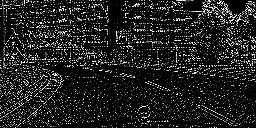
\includegraphics[width=\textwidth]{pictures/vq-f8-n256_latent_channel_4.png}
                \end{minipage}
            \end{figure}
    

\printbibliography

\end{document}
